\begin{ex}%[2D3H2-2]
% nguon: Archive/SP_SauLuoi_2024-2025/SP_HKI/2-TN-DS-TLN-SGD-BacNinh-HKI-NH24-25.tex #1

	Kết quả kiểm tra môn Tiếng Anh (cùng một đề) của học sinh hai lớp 12A và 12B được cho lần lượt bởi mẫu số liệu ghép nhóm ở Bảng A và Bảng B.	
	\begin{center}
		\begin{tabular}{cc}	
			
			\begin{tabular}{|c|c|c|}
				\hline
				\textbf{Nhóm} & \textbf{Giá trị đại diện} & \textbf{Tần số} \\
				\hline
				$[0; 2)$ & $1$ & $3$ \\
				\hline
				$[2; 4)$ & $3$ & $5$ \\
				\hline
				$[4; 6)$ & $5$ & $5$ \\
				\hline
				$[6; 8)$ & $7$ & $25$ \\
				\hline
				$[8; 10)$ & $9$ & $2$ \\
				\hline
				& & $n = 40$ \\
				\hline
			\end{tabular}&
			\begin{tabular}{|c|c|c|}
				\hline
				\textbf{Nhóm} & \textbf{Giá trị đại diện} & \textbf{Tần số} \\
				\hline
				$[0; 2)$ & $1$ & $1$ \\
				\hline
				$[2; 4)$ & $3$ & $4$ \\
				\hline
				$[4; 6)$ & $5$ & $15$ \\
				\hline
				$[6; 8)$ & $7$ & $16$ \\
				\hline
				$[8; 10)$ & $9$ & $4$ \\
				\hline
				& & $n = 40$ \\
				\hline
			\end{tabular}  \\
			& \\
			\textbf{Bảng A}&\textbf{Bảng B}  \\
		\end{tabular}
	\end{center}
	\choiceTF
	{Độ lệch chuẩn của mẫu số liệu lớp 12A nhỏ hơn $2$}
	{\True Phương sai của mẫu số liệu lớp 12B lớn hơn $3$}
	{\True Số trung bình cộng của hai mẫu số liệu trên bằng nhau}
	{\True Dựa vào độ lệch chuẩn ta thấy điểm thi của học sinh lớp 12B đồng đều hơn lớp 12A}
	\loigiai{
		\begin{itemize}
			\item 
			\textbf{Số trung bình cộng của mẫu số liệu lớp 12A:}
			\[
			\overline{x}_A = \dfrac{3 \cdot 1 + 5 \cdot 3 + 5 \cdot 5 + 25 \cdot 7 + 2 \cdot 9}{40} = \dfrac{227}{40} = 5,9.
			\]
			\item \textbf{Phương sai và độ lệch chuẩn của mẫu số liệu lớp 12A:}
			\begin{eqnarray*}
				s_A^2 &=& \dfrac{1}{40} \left[3 \cdot (1 - 5,9)^2 + 5 \cdot (3 - 5,9)^2 + 5 \cdot (5 - 5,9)^2\right. \\
				&&\left.+ 25 \cdot (7 - 5,9)^2 + 2 \cdot (9 - 5,9)^2\right]\\
				&=&  4{,}19.
			\end{eqnarray*}
			Độ lệch chuẩn của mẫu số liệu lớp 12A là
			\[
			s_A = \sqrt{4{,}19} \approx 2{,}05.
			\]
			\item \textbf{Số trung bình cộng của mẫu số liệu lớp 12B:}
			\[
			\overline{x}_B = \dfrac{1 \cdot 1 + 4 \cdot 3 + 15 \cdot 5 + 16 \cdot 7 + 4 \cdot 9}{40} = \dfrac{227}{40} = 5{,}9.
			\]			
			\textbf{Phương sai và độ lệch chuẩn của mẫu số liệu lớp 12B:}
			\begin{eqnarray*}
				s_B^2 &=& \dfrac{1}{40} \left[1 \cdot (1 - 5,9)^2 + 4 \cdot (3 - 5,9)^2 + 15 \cdot (5 - 5,9)^2\right.\\
				&&\left.+ 16 \cdot (7 - 5,9)^2 + 4 \cdot (9 - 5,9)^2\right] \\
				&=&3{,}19.
			\end{eqnarray*}
			Độ lệch chuẩn của mẫu số liệu lớp 12B là
			\[
			s_B = \sqrt{3{,}19} \approx 1{,}79.
			\]
		\end{itemize}
		Khi đó 
		\begin{itemchoice} 
			\itemch \textbf{Sai}.\\
			Độ lệch chuẩn của lớp 12A là $2{,}05$, lớn hơn $2$ 
			\itemch \textbf{Đúng}.\\
			Phương sai của lớp 12B là $3{,}19$, nhỏ hơn $3$
			\itemch \textbf{Đúng.} \\
			Số trung bình cộng của hai mẫu bằng nhau và bằng $5,9$.
			\itemch \textbf{Đúng.} \\
			Độ lệch chuẩn của lớp 12B nhỏ hơn lớp 12A, do đó điểm thi của lớp 12B đồng đều hơn lớp 12A.
		\end{itemchoice}
	}
\end{ex}

\begin{bt}%[2D3V1-4]
% nguon: Archive/SP_SauLuoi_2024-2025/SP_HKI/2-TN-DS-TLN-SGD-BacNinh-HKI-NH24-25.tex #4
%[Dự án đề kiểm tra HK1,Toán 12 Bắc Ninh]%[Bùi Lợi-GV21]
	Một siêu thị thống kê số tiền (đơn vị: chục nghìn đồng) mà $44$ khách hàng mua hàng ở siêu thị đó trong một ngày. Số liệu được ghi lại trong bảng sau:
	\begin{center}
		\begin{tabular}{|c|c|c|c|c|c|c|c|}
			\hline 
			Nhóm & $[40;45)$ & $[45;50)$ & $[50;55)$ & $[55;60)$ & $[60;65)$ & $[65;70)$ &  \\ 
			\hline
			Tần số & $4$ & $14$ & $8$ & $10$ & $6$ & $2$ & $n=44$ \\
			\hline
		\end{tabular}
	\end{center}
	Hiệu giữa khoảng biến thiên và khoảng tứ phân vị của bảng số liệu trên bằng bao nhiêu?
	\shortans{19}
	\loigiai{
		Ta có $n=44$.\\
		Khoảng biến thiên của mẫu số liệu là: $R=70-40=30$.\\
		Gọi $x_1$, $x_2$,$\cdots$, $x_{44}$ lần lượt là số tiền (đơn vị: chục nghìn đồng) của $44$ khách hàng theo thứ tự không giảm.\\
		Tứ phân vị thứ nhất của dãy số liệu là $\dfrac{1}{2}\left(x_{11}+x_{12}\right)$ thuộc nhóm $[45;50)$ nên tứ phân vị thứ nhất của mẫu số liệu là
		\[
		Q_1 = 45+\dfrac{\dfrac{44}{4}-4}{14}\cdot (50-45) = 47{,}5.
		\]
		Tứ phân vị thứ ba của dãy số liệu là $\dfrac{1}{2}\left(x_{33}+x_{34}\right)$ thuộc nhóm $[55;60)$ nên tứ phân vị thứ ba của mẫu số liệu là
		\[
		Q_3=55+\dfrac{\dfrac{3\cdot 44}{4}-(4+14+8)}{10}\cdot (65-60) = 58{,}5.
		\]
		Khi đó khoảng tứ phân vị là $\Delta_Q = Q_3 - Q_1 = 11$.\\
		Vậy, kết quả cần tìm là $R-\Delta_Q = 30-11=19$.
	}
\end{bt}

\begin{bt}%[2D3V2-2]
% nguon: Archive/SP_SauLuoi_2024-2025/SP_HKI/2-TN-DS-TLN-SGD-BacNinh-HKI-NH24-25.tex #7
%[2-TN-DS-TLN-SGK-BacNinh-HKI-NH24-25]%[Tư Đô Nguyên]
	Tốc độ của $20$ xe hơi khi đi qua một trạm kiểm tra tốc độ (đơn vị: km/h) được thống kê lại như sau:
	\begin{center}
		\begin{tabular}{|c|c|c|c|c|c|c|c|c|c|}
			\hline $42$ & $43{,}4$ & $43{,}4$ & $46{,}5$ & $46{,}7$ & $46{,}8$ & $47{,}5$ & $47{,}7$ & $48{,}1$ & $48{,}4$ \\
			\hline $50{,}8$ & $52{,}1$ & $52{,}7$ & $53{,}9$ & $54{,}8$ & $55{,}6$ & $57{,}5$ & $59{,}6$ & $60{,}3$ & $61{,}1$ \\
			\hline
		\end{tabular}
	\end{center}
	Ghép nhóm mẫu số liệu trên với nhóm đầu tiên là $[42 ; 46)$ và độ dài mỗi nhóm bằng $4$. Độ lệch chuẩn của mẫu ghép nhóm này bằng bao nhiêu (kết quả làm tròn đến hàng phần trăm)?
	\shortans{5,15}
	\loigiai{
		Mẫu số liệu ghép nhóm của bảng số liệu trên với nhóm đầu tiên là $[42 ; 46)$ và độ dài mỗi nhóm bằng $4$:
		\begin{center}
			\begin{tabular}{|l|c|c|c|c|c|}
				\hline \textbf{Tốc độ (km/h)} & $[42 ; 46)$ & $[46 ; 50)$ & $[50 ; 54)$ & $[54 ; 58)$ & $[58 ; 62)$ \\
				\hline \textbf{Giá trị đại diện} & $44$ & $48$ & $52$ & $56$ & $60$ \\
				\hline \textbf{Số xe} & $3$ & $7$ & $4$ & $3$ & $3$ \\
				\hline
			\end{tabular}
		\end{center}
		Tốc độ trung bình:
		\[\dfrac{3\cdot 44+7\cdot48+4\cdot52+3\cdot56+3\cdot60}{20}=51{,}2.\]
		Phương sai của mẫu số liệu ghép nhóm:
		$$
		S^2=\dfrac{1}{20}\left(3\cdot 44^2+7\cdot48^2+4\cdot52^2+3\cdot56^2+3\cdot60^2\right)-51{,}2^2=26{,}56.
		$$
		Độ 1ệch chuẩn:
		$$
		S=\sqrt{26{,}56} \approx 5{,}15.
		$$
	}
\end{bt}

\begin{ex}%[2D3H2-3]
% nguon: Archive/SP_SauLuoi_2024-2025/SP_HKI/2-TN-DS-TLN-THPT-ThienPhuoc-DongNai-HKI-NH24-25.tex #13
%[2-TN-DS-TLN-THPT-ThienPhuoc-DongNai-HKI-NH24-25 - Phúc Chương]
	An tìm hiểu hàm lượng chất béo (đơn vị: gam) có trong $100$ g mỗi loại thực phẩm. Sau khi thu thập dữ liệu về $60$ loại thực phẩm, An lập được bảng thống kê
	\begin{center}
		\begin{tabular}{|l|c|c|c|c|c|c|}
			\hline
			Hàm lượng chất béo (g) & [2;6) & [6;10) & [10;14) & [14;18) & [18;22) & [22;26) \\ \hline
			Tần số & 2 & 6 & 10 & 13 & 16 & 13 \\ \hline
		\end{tabular}
	\end{center}
	\choiceTF
	{\True Hàm lượng chất béo trung bình có trong $100$ g thực phẩm là $16{,}93$ g (kết quả làm tròn đến hàng phần trăm)}
	{Trung vị của mẫu số liệu ghép nhóm trên thuộc nhóm $[10;14)$}
	{Tứ phân vị thứ ba của mẫu số liệu ghép nhóm trên là $Q_3=21{,}5$ g}
	{Độ lệch chuẩn của mẫu số liệu ghép nhóm trên là $5{,}56$ g (kết quả làm tròn đến hàng phần trăm)}
	\loigiai{
		\begin{itemchoice}
			\itemch \textbf{Đúng}.\\
			Ta có bảng tần số với giá trị đại diện sau:
			\begin{center}
				\begin{tabular}{|l|c|c|c|c|c|c|}
					\hline
					Hàm lượng chất béo (g) & [2;6) & [6;10) & [10;14) & [14;18) & [18;22) & [22;26) \\
					\hline Giá trị đại diện & 4 & 8 & 12 & 16 & 20 & 24 \\
					\hline
					Tần số & 2 & 6 & 10 & 13 & 16 & 13  \\ \hline
				\end{tabular}
			\end{center}
			Từ bảng trên, ta tính được số trung bình của mẫu số liệu trên là $\overline{x} \approx 16{,}93$.
			\itemch \textbf{Sai}.\\
			Mẫu số liệu trên có $60$ số liệu, do đó nhóm chứa trung vị của mẫu số liệu là nhóm chứa số liệu ở vị trí thứ 30 và 31 của mẫu số liệu, tức là nhóm $[14;18)$.
			\itemch \textbf{Sai}.\\
			Nhóm tứ phân vị thứ ba là nhóm $[18;22)$. Ta có
			$$Q_3=18+\dfrac{\dfrac{3n}{4}-(2+6+10+13)}{16}\cdot(22-18)=19{,}75.$$
			\itemch \textbf{Sai}.\\
			Độ lệch chuẩn của mẫu số liệu trên là $s\approx5{,}58$.
		\end{itemchoice}
	}
\end{ex}

\begin{bt}%[2D3H1-3]
% nguon: Archive/SP_SauLuoi_2024-2025/SP_HKI/2-TN-DS-TLN-THPT-ThienPhuoc-DongNai-HKI-NH24-25.tex #14
%[2-TN-DS-TLN-THPT-ThienPhuoc-DongNai-HKI-NH24-25]%[Tran Ngoc Thanh]
	Thống kê số lượt xem mỗi video trong 35 video của một bạn Youtuber mới lập kênh được một tháng:
\begin{center}
		\begin{tabular}{|c|c|c|c|c|c|}
		\hline
		Số lượt xem & {$[200;500)$} & {$[500;500)$} & $[500;1100)$ & $[1100;1400)$ & $[1400;1700)$ \\
		\hline
		Số video & 4 & 7 & 2 & 15 & 7 \\
		\hline
	\end{tabular}
\end{center}
	Tứ phân vị thứ ba của mẫu số liệu ghép nhóm trên bằng bao nhiêu?
	\shortans{1365}
\loigiai{
	Ta có $ Q_{3}=x_{27} \in [1100; 1400)$.\\
	Suy ra $Q_{3}=1100+\dfrac{\dfrac{3\cdot 35}{4}-13}{15}\cdot 300= 1365$.	
	}
	\end{bt}

\begin{ex}%[2D3N1-2]
% nguon: Archive/SP_SauLuoi_2024-2025/SP_HKI/2-TN-DS-TLN-THPT-PhaHuyChu-HaNoi-HKI-NH24-25.tex #32
%[2-TN-DS-TLN-Phan Huy Chú-Hà Nội-HKI-24-25]%[Nguyễn Hoàng Anh]
	Trong thực hành đo hiệu điện thế của mạch điện, An và Bình đã dùng hai Vôn kế khác nhau để đo, mỗi bạn tiến hành đo $10$ lần và cho kết quả như sau
	\begin{center}
		\renewcommand{\arraystretch}{1.3}
		\begin{tabular}{|>{\centering\arraybackslash}p{5.5cm}|>{\centering\arraybackslash}p{2cm}|>{\centering\arraybackslash}p{2cm}|>{\centering\arraybackslash}p{2cm}|>{\centering\arraybackslash}p{2cm}|}
			\hline
			\textbf{Hiệu điện thế đo được (Vôn)} & $[3{,}85; 3{,}90)$&$[3{,}90; 3{,}95)$&$[3{,}95; 4{,}00)$&$[4{,}00; 4{,}05)$ \\ \hline
			\textbf{Số lần An đo}  & 1 & 6 & 2 & 1 \\ \hline
			\textbf{Số lần Bình đo}  & 1 & 3 & 4 & 2 \\ \hline
		\end{tabular}
		\renewcommand{\arraystretch}{1}
	\end{center}
	\choiceTF
	{\True Khoảng biến thiên của hai mẫu số liệu là như nhau}
	{Giá trị trung bình mẫu số liệu của hai bạn bằng nhau}
	{\True Các kết quả đo được của An ổn định hơn của Bình}
	{Độ lệnh chuẩn của mẫu số liệu về kết quả đo của An lớn hơn của Bình}
	\loigiai{
		\begin{itemchoice}
			\itemch \textbf{Đúng}.\\
			Khoảng biến thiên mẫu số liệu của An là $4{,}05-3{,}85=0{,}2$.\\
			Khoảng biến thiên mẫu số liệu của An là $4{,}05-3{,}85=0{,}2$.\\
			Vậy khoảng biến thiên của hai mẫu số liệu là như nhau.
			\itemch \textbf{Sai}.
			Ta có
			\begin{center}
				\renewcommand{\arraystretch}{1.3}
				\begin{tabular}{|>{\centering\arraybackslash}p{5.5cm}|>{\centering\arraybackslash}p{2cm}|>{\centering\arraybackslash}p{2cm}|>{\centering\arraybackslash}p{2cm}|>{\centering\arraybackslash}p{2cm}|}
					\hline
					\textbf{Hiệu điện thế đo được (Vôn)} & $[3{,}85; 3{,}90)$&$[3{,}90; 3{,}95)$&$[3{,}95; 4{,}00)$&$[4{,}00; 4{,}05)$ \\ \hline
					\textbf{Giá trị đại diện}  & $3{,}875$ & $3{,}925$ & $3{,}975$ & $4{,}025$ \\ \hline
					\textbf{Số lần An đo}  & 1 & 6 & 2 & 1 \\ \hline
					\textbf{Số lần Bình đo}  & 1 & 3 & 4 & 2 \\ \hline
				\end{tabular}
			\end{center}
			\renewcommand{\arraystretch}{1}
			Giá trị trung bình mẫu số liệu của An là
			\begin{center}
				$\overline{x}_{A}=\dfrac{1\cdot 3{,}875+6\cdot 3{,}925+2\cdot 3{,}975+1\cdot 4{,}025}{10}=3{,}94$.
			\end{center}
			Giá trị trung bình mẫu số liệu của Bình là
			\begin{center}
				$\overline{x}_{B}=\dfrac{1\cdot 3{,}875+3\cdot 3{,}925+4\cdot 3{,}975+2\cdot 4{,}025}{10}=3{,}96$.
			\end{center}
			\itemch \textbf{Đúng}.\\
			Phương sai mẫu số liệu của An là
			\begin{eqnarray*}
				\sigma^2_{A}&=&\dfrac{1\cdot (3{,}875-3{,}94)^2+6\cdot (3{,}925-3{,}94)^2+2\cdot (3{,}975-3{,}94)^2+1\cdot (4{,}025-3{,}94^2)}{10}\\
				&=&0{,}001525.
			\end{eqnarray*}
			Phương sai mẫu số liệu của Bình là
			\begin{eqnarray*}
				\sigma^2_{B}&=&\dfrac{1\cdot (3{,}875-3{,}96)^2+3\cdot (3{,}925-3{,}96)^2+2\cdot (3{,}975-3{,}96)^2+4\cdot (4{,}025-3{,}96^2)}{10}\\
				&=&0{,}002025.
			\end{eqnarray*}
			$\sigma^2_{A}<\sigma^2_{B}$ nên các kết quả đo được của An ổn định hơn của Bình.
			\itemch \textbf{Sai}.\\
			Độ lệch chuẩn của mẫu số liệu của An là $\sigma_{A}=\sqrt{\sigma^2_{A}}=\sqrt{0{,}001525} \approx 0{,}039$.\\
			Độ lệch chuẩn của mẫu số liệu của Bình là $\sigma_{B}=\sqrt{\sigma^2_{B}}=\sqrt{0{,}002025} = 0{,}045$.\\
			Suy ra $\sigma_{A}<\sigma_{B}$.
			
		\end{itemchoice}
	}
\end{ex}

\begin{bt}%[2D3H1-3]
% nguon: Archive/SP_SauLuoi_2024-2025/SP_HKI/2-TN-DS-TLN-THPT-PhaHuyChu-HaNoi-HKI-NH24-25.tex #38
%[Lớp 12 – Đề thi học kì 1]%[Thanh Phát]
	Điều tra của chủ nông trường về chiều cao (đơn vị: mét) của $200$ cây keo $3$ năm tuổi được cho ở biểu đồ dưới đây
	\begin{center}
		\begin{tikzpicture}[>=stealth,line join=round,line cap=round,font=\footnotesize,scale=0.8,line width=1pt]
			\draw[->] (0,0)--(0,8)node[left]{\text{Số cây}};
			\draw[->] (0,0)--(10.5,0)node[below right]{\text{Chiều cao (m)}};
			\draw[fill=black] (0,0) node[left]{$0$};
			\foreach \y in {1, 2, 3, 4, 5, 6, 7} {\draw (0.05,\y) -- (-0.05,\y);
				\node[left] at (-0.05, \y) {$\y 0$};}
			\draw[fill=blue!20] (0,0) rectangle (2,2);
			\draw[fill=blue!20] (2,0) rectangle (4,3.5);
			\draw[fill=blue!20] (4,0) rectangle (6,6);
			\draw[fill=blue!20] (6,0) rectangle (8,5.5);
			\draw[fill=blue!20] (8,0) rectangle (10,3);
			\node [below] at (1,0){$[8,5;8,8)$};
			\node [below] at (3,0){$[8,8;9,1)$};
			\node [below] at (5,0){$[9,1;9,4)$};
			\node [below] at (7,0){$[9,4;9,7)$};
			\node [below] at (9,0){$[9,7;10)$};
			\node [above] at (1,2){$20$};
			\node [above] at (3,3.5){$35$};
			\node [above] at (5,6){$60$};
			\node [above] at (7,5.5){$55$};
			\node [above] at (9,3){$30$};
			\path (5.25,8.5) node {\normalsize{\textbf{Chiều cao \boldmath{200} cây keo \boldmath{3} năm tuổi}}};
		\end{tikzpicture}
	\end{center}
	Tìm khoảng tứ phân vị của mẫu số liệu (\textit{làm tròn kết quả đến hàng phần trăm}).
	\shortans{0{,}53}
	\loigiai{Ta có
		\begin{eqnarray*}
			Q_1&=&8{,}8 +\dfrac{\tfrac{200}{4}-20}{35}\cdot (9{,}1- 8{,}8)=\dfrac{317}{35}.\\
			Q_3&=&9{,}4 + \dfrac{\tfrac{3\cdot 200}{4}-(20+35+60)}{55}\cdot (9{,}7 - 9{,}4)=\dfrac{211}{22}.
		\end{eqnarray*}
		Khi đó khoảng biến thiên $\Delta Q=Q_3 - Q_1= \dfrac{211}{22} - \dfrac{317}{35}=\dfrac{411}{770}\approx 0{,}53$.
	}
\end{bt}

\begin{ex}%[2D3H2-2]
% nguon: Archive/SP_SauLuoi_2024-2025/SP_HKI/2-TN-DS-TLN-TL-THPT-TranPhu-VungTau-HKI-NH24-25.tex #50
%[Dự án đề kiểm tra Toán 12 HKI NH24-25- Võ Thị Thùy Trang]%[THPT - TRẦN PHÚ]
	Một trung tâm Y tế thống kê một số học sinh bị cận thị ở trường THPT thì có $87$ học sinh bị cận được ghi nhận lại ở bảng sau
	\begin{center}
		\begin{tabular}{|c|c|c|c|c|c|}
			\hline
			Thời gian & {$[0{,}25;0{,}75)$} &{$[0{,}75;1{,}25)$} & {$[1{,}25;1{,}75)$} & {$[1{,}75; 2{,}25)$} & {$[2{,}25;2{,}75)$} \\
			\hline
			Số lần & $25$ & $32$ & $14$ & $12$ & $4$ \\
			\hline
		\end{tabular}
	\end{center}
	\choiceTF
	{\True Khoảng biến thiên của mẫu số liệu ghép nhóm trên là $2{,}5$}
	{Khoảng tứ phân vị của mẫu số liệu ghép nhóm trên lớn hơn $1$}
	{Phương sai của mẫu số liệu trên lớn hơn $0{,}4$}
	{Độ lệch chuẩn của mẫu số liệu trên bé hơn $0{,}5$}
	\loigiai{
		\begin{itemchoice}
			\itemch \textbf{Đúng}.\\
			Khoảng biến thiên của mẫu số liệu ghép nhóm trên là $2{,}75-0{,}25=2{,}5$.
			\itemch \textbf{Sai}.\\
			\begin{itemize}
				\item Tứ phân vị thứ nhất là $Q_1=0{,}25+\dfrac{\dfrac{87}{4}-0}{25}\cdot(0{,}75-0{,}25)=\dfrac{137}{200}$.
				\item Tứ phân vị thứ ba là $Q_3=1{,}25+\dfrac{\dfrac{3\cdot 87}{4}-57}{14}\cdot(1{,}75-1{,}25)=\dfrac{173}{112}$.
				\item Khoảng tứ phân vị là $\Delta Q=Q_3-Q_1=\dfrac{173}{112}-\dfrac{137}{200}=\dfrac{2407}{2800}\approx 0{,}86<1$.
			\end{itemize}
			\itemch \textbf{Sai}.\\
			\begin{center}
				\begin{tabular}{|c|c|c|c|c|c|}
					\hline
					Thời gian & {$[0{,}25;0{,}75)$} &{$[0{,}75;1{,}25)$} & {$[1{,}25;1{,}75)$} & {$[1{,}75; 2{,}25)$} & {$[2{,}25;2{,}75)$} \\
					\hline
					Giá trị đại diện & $0{,}5$ & $1$ & $1{,}5$ & $2$ & $2{,}5$ \\
					\hline
					Số lần & $25$ & $32$ & $14$ & $12$ & $4$ \\
					\hline
				\end{tabular}
			\end{center}
			Giá trị trung bình của mẫu số liệu là\\ $\overline{x}=\dfrac{0{,}5\cdot 25+1\cdot 32+1{,5}\cdot 14+2\cdot 12+2{,5}\cdot 4}{87}=\dfrac{199}{174}$.\\
			Phương sai của mẫu số liệu là\\ $s^2=\dfrac{1}{87}\left(25\cdot (0{,}5)^2+32\cdot 1^2+14\cdot (1{,}5)^2+12\cdot 2^2+4\cdot (2{,}5)^2\right)-\left(\dfrac{199}{174}\right)^2\approx 0{,}33<0{,}4$.
			\itemch \textbf{Sai}.\\
			Độ lệch chuẩn của mẫu số liệu trên là  $s=\sqrt{s^2}\approx 0{,}58>0{,}5$.
		\end{itemchoice}
	}
\end{ex}

\begin{bt}%[2D3H1-3]
% nguon: Archive/SP_SauLuoi_2024-2025/SP_HKI/2-TN-DS-TLN-THPT-NguyenKhuyen-AnGiang-HKI-NH24-25.tex #63
%[Đề thi HK1 lớp 12 THPT Nguyễn Khuyến-An Giang NH 24-25]%[Nguyễn Tấn Linh]
	Cô Hà thống kê lại đường kính thân gỗ của một số cây xoan đào 6 năm tuổi được trồng ở một lâm trường ở bảng sau.
	\begin{center}
		\begin{tabular}{|c|c|c|c|c|c|}
			\hline
			\textbf{Đường kính (cm)} & $[40;45)$ & $[45;50)$ & $[50;55)$ & $[55;60)$ & $[60;65)$ \\ \hline
			\textbf{Tần số}          & $5$           & $20$          & $18$          & $7$           & $3$           \\ \hline
		\end{tabular}
	\end{center}
	Hãy xác định khoảng tứ phân vị của mẫu số liệu ghép nhóm trên (kết quả làm tròn đến hàng phần trăm).\shortans{$7,03$}
	\loigiai
	{
		\begin{center}
			\begin{tabular}{|c|c|c|c|c|c|}
				\hline
				\textbf{Đường kính (cm)} & $[40;45)$ & $[45;50)$ & $[50;55)$ & $[55;60)$ & $[60;65)$ \\ \hline
				\textbf{Tần số}          & $5$           & $20$          & $18$          & $7$           & $3$           \\ \hline
				\textbf{Tần số tích lũy} & $5$ & $25$ & $43$ & $50$ & $53$\\\hline
			\end{tabular}
		\end{center}
		Ta có $\dfrac{n}{4}=13,25$ nên nhóm chứa tứ phân vị thứ nhất là $[45;50)$.\\
		Tứ phân vị thứ nhất của mẫu số liệu là
		\[Q_1=45+\dfrac{\dfrac{53}{4}-5}{20}(50-45)=\dfrac{753}{16}. \]
		Ta có $\dfrac{3n}{4}=39,75$ nên nhóm chứa tứ phân vị thứ ba là $[50;55)$.\\
		Tứ phân vị thứ ba của mẫu số liệu là
		\[Q_3=50+\dfrac{\dfrac{3\cdot 53}{4}-25}{18}(55-50)=\dfrac{3895}{72}. \]
		Khoảng tứ phân vị của mẫu số liệu là $\Delta_Q=Q_3-Q_1=\dfrac{1013}{144}\approx 7{,}03$.
	}
\end{bt}

\begin{ex}%[2D3N1-3]
% nguon: Archive/SP_SauLuoi_2024-2025/SP_HKI/2-TN-DS-TLN-THPT-MarieCurie-HCM-HKI-NH24-25.tex #69
%[Dự án A - HKI - THPT Marie Curie - TP. Hồ Chí Minh - 24-25]%[Nguyễn Ngọc Huy Trường]
	Khảo sát thời gian tự học của học sinh lớp 12A tại một trường X trong một tuần được thống kê ở bảng sau
	\begin{center}
		\begin{tabular}{|c|c|c|c|c|c|c|}
			\hline
			Thời gian (giờ) & $[5;7)$ & $[7;9)$ & $[9;11)$ & $[11;13)$ & $[13;15)$ & $[15;17)$ \\
			\hline
			Số học sinh & $8$ & $7$ & $9$ & $12$ & $7$ & $2$ \\
			\hline
		\end{tabular}
	\end{center}
	\choiceTF
	{\True Cỡ mẫu $n=45$}
	{\True Độ lệch chuẩn có cùng đơn vị với đơn vị của mẫu số liệu}
	{Tứ phân vị thứ nhất của mẫu số liệu ghép nhóm trên thuộc nhóm $[9;11)$}
	{Khoảng tứ phân vị của mẫu số liệu ghép nhóm bằng $5{,}2$. (làm tròn kết quả đến phần mười)}
	\loigiai{
		Ta có bảng sau
		\begin{center}
			\begin{tabular}{|c|c|c|c|c|c|c|}
				\hline
				Giá trị đại diện & $6$ & $8$ & $10$ & $12$ & $14$ & $16$ \\
				\hline
				Thời gian (giờ) & $[5;7)$ & $[7;9)$ & $[9;11)$ & $[11;13)$ & $[13;15)$ & $[15;17)$ \\
				\hline
				Số học sinh & $8$ & $7$ & $9$ & $12$ & $7$ & $2$ \\
				\hline
				Tần số tích luỹ & $8$ & $15$ & $24$ & $36$ & $43$ & $45$ \\
				\hline
			\end{tabular}
		\end{center}
		\begin{itemchoice}
			\itemch \textbf{Đúng}. $n = 8+7+9+12+7+2=45$. \\
			\itemch \textbf{Đúng}. Ta có độ lệch chuẩn có cùng đơn vị với đơn vị của mẫu số liệu.
			\itemch \textbf{Sai}. Ta có $\dfrac{n}{4} = 11{,}25$. \\
			Vậy tứ phân vị thứ nhất của mẫu số liệu ghép nhóm trên thuộc nhóm $[7;9)$.
			\itemch \textbf{Sai}. Ta có $$Q_1 = 7 + \dfrac{11{,}25-8}{7}\cdot (9-7) = \dfrac{111}{14}.$$
			Ta có $\dfrac{3n}{4} = 33{,}75$. \\
			Suy ra tứ phân vị thứ ba của mẫu số liệu ghép nhóm trên thuộc nhóm $[11;13)$. \\
			Do đó
			$$Q_3 = 11 + \dfrac{33{,}75 - 24}{12}\cdot (13-11) = \dfrac{101}{8}.$$
			Vậy khoảng tứ phân vị của mẫu số liệu ghép nhóm là $$\Delta_Q = Q_3 - Q_1 = \dfrac{111}{14} - \dfrac{101}{8} \approx 4{,}7.$$
		\end{itemchoice}
	}
\end{ex}

\begin{bt}%[2D3H2-2]
% nguon: Archive/SP_SauLuoi_2024-2025/SP_HKI/2-TN-DS-TLN-THPT-MarieCurie-HCM-HKI-NH24-25.tex #75
%[Dự án đề kiểm tra Toán 12 GHKI NH23-24- Trần Xuân Hòa]%[THPT MarieCurie - Tp HCM]
Thống kê mật độ dân số (đơn vị: người/km$^2$) của $23$ tỉnh, thành phố thuộc vùng Trung du và miền núi phía Bắc, Đồng bằng sông Hồng (không kể thành phố Hà Nội và tỉnh Bắc Ninh) trong năm $2\,021$.
\begin{flushright}
	(Nguồn: Niên giám Thống kê $2\,021$, NXB Thống kê, $2\,022$).
\end{flushright}
\begin{center}
\begin{tabular}{|c|c|c|c|c|c|c|c|}
	\hline Mật độ& {$[0 ; 200)$} & {$[200 ; 400)$} & {$[400 ; 600)$} & {$[600 ; 800)$} & {$[800 ; 1\,000)$} & {$[1\,000 ; 1\,200)$} & {$[1\,200 ; 1\,400)$} \\
	\hline Tần số & $13$ & $2$ & $2$ & $0$ & $1$ & $3$ & $2$ \\
	\hline
\end{tabular}	
\end{center}
Tính độ lệch chuẩn của mẫu số liệu ghép nhóm. (Kết quả làm tròn đến hàng đơn vị).
\shortans{$444$}
	\loigiai{
	Ta có\\
	\begin{tabular}{|c|c|c|c|c|c|c|c|}
		\hline Mật độ& {$[0 ; 200)$} & {$[200 ; 400)$} & {$[400 ; 600)$} & {$[600 ; 800)$} & {$[800 ; 1\,000)$} & {$[1\,000 ; 1\,200)$} & {$[1\,200 ; 1\,400)$} \\
		\hline Tần số & $13$ & $2$ & $2$ & $0$ & $1$ & $3$ & $2$ \\
		\hline GT đại diện & $100$ & $300$ & $500$ & $700$ & $900$ & $1\,100$ & $1\,300$ \\
		\hline
	\end{tabular}\\
	Số trung bình 
	\[\overline{x}=\dfrac{13\cdot 100+2\cdot 300+2\cdot 500+0\cdot 700+1\cdot 900+3\cdot 1\,100+2\cdot 1\,300}{23}=\dfrac{9\,700}{23} \approx 421{,}74.\]
	Phương sai
	\begin{eqnarray*}
		&s^2&=\dfrac{13(100 - 421,74)^2 + 2(300 - 421,74)^2 + 2(500 - 421,74)^2+0(700 - 421,74)^2}{23}\\
		&&+\dfrac{1(900 - 421,74)^2 + 3(1\,100 - 421,74)^2 + 2(1\,300 - 421,74)^2}{23}\\
		&s^2&\approx 197\,288{,}37.
	\end{eqnarray*}
	Độ lệch chuẩn $s=\sqrt{s^2}\approx 444$.
	}
\end{bt}

\begin{ex}%[2D3H2-2]
% nguon: Archive/SP_SauLuoi_2024-2025/SP_HKI/2-TN-DS-TLN-THPT-ThiXaQuangTri-QuangTri-HKI-NH24-25.tex #79
%[Dự án đề kiểm tra Toán 12 HKI NH24-25-Nguyễn Hữu Duy]%[THPT Thị Xã Quảng Trị - Quảng Trị]
	Bảng số liệu ghép nhóm sau cho biết cân nặng của $42$ học sinh lớp $12C$.
	\begin{center}
		\begin{tabular}{|c|c|c|c|c|c|c|}
			\hline 
			\textbf{Cân nặng (kg)} & $[40{,}5;45{,}5)$ & $[45{,}5;50{,}5)$ & $[50{,}5;55{,}5)$ & $[55{,}5;60{,}5)$ & $[60{,}5;65{,}5)$ & $[65{,}5;70{,}5)$\\
			\hline 
			\textbf{Số học sinh} & $10$ & $7$ & $16$ & $4$ & $2$ & $3$ \\
			\hline
		\end{tabular}
	\end{center}
	\choiceTF
	{\True Giá trị đại diện của nhóm $[40{,}5;45{,}5)$ là $43$}
	{\True Số trung bình của mẫu số liệu ghép nhóm trên là $\overline{x}=\dfrac{1088}{21}$}
	{Phương sai của mẫu số liệu ghép nhóm trên là $s^2\approx 1{,}57$}
	{\True Độ lệch chuẩn của mẫu số liệu ghép nhóm trên là $s\approx 7{,}06$}
	\loigiai{
		Ta lập lại bảng số liệu như sau
		\begin{center}
			\begin{tabular}{|c|c|c|c|c|c|c|}
				\hline 
				\textbf{Cân nặng (kg)} & $[40{,}5;45{,}5)$ & $[45{,}5;50{,}5)$ & $[50{,}5;55{,}5)$ & $[55{,}5;60{,}5)$ & $[60{,}5;65{,}5)$ & $[65{,}5;70{,}5)$\\
				\hline 
				\textbf{Cân nặng đại diện} & $43$ & $48$ & $53$ & $58$ & $63$ & $68$\\
				\hline 
				\textbf{Số học sinh} & $10$ & $7$ & $16$ & $4$ & $2$ & $3$ \\
				\hline
			\end{tabular}
		\end{center}
		Cỡ mẫu $n=42$.
		\begin{itemchoice}
			\itemch \textbf{Đúng}.\\
			Giá trị đại diện của nhóm $[40{,}5;45{,}5)$ là $43$.
			\itemch \textbf{Đúng}.\\
			Số trung bình của mẫu số liệu ghép nhóm trên là
			\begin{align*}
				\overline{x}=\dfrac{43\cdot 10+48\cdot 7+53\cdot 16+58\cdot 4+63\cdot 2+68\cdot 3}{42}
				= \dfrac{1088}{21}.
			\end{align*}
			\itemch \textbf{Sai}.\\
			Phương sai của mẫu số liệu ghép nhóm trên là
			\begin{align*}
				s^2=\dfrac{43^2\cdot 10+48^2\cdot 7+53^2\cdot 16+58^2\cdot 4+63^2\cdot 2+68^2\cdot 3}{42} - \overline{x}^2
				= \dfrac{21950}{441}\approx 49{,}77.
			\end{align*}
			\itemch \textbf{Đúng}.\\
			Độ lệch chuẩn của mẫu số liệu ghép nhóm trên là $s=\sqrt{\dfrac{21950}{441}}=\dfrac{5\sqrt{878}}{21}\approx 7{,}06$.
		\end{itemchoice}
	}
\end{ex}

\begin{bt}%[2D3H1-3]
% nguon: Archive/SP_SauLuoi_2024-2025/SP_HKI/2-TN-DS-TLN-THPT-ChuyenLeHongPhong-HCM-HKI-NH24-25.tex #89
%[Dự án đề kiểm tra Toán 12 HKI Dot 04 NH24-25-Lê Hữu Kiệt]%[THPT Chuyên Lê Hồng Phong - TP Hồ Chí Minh]
	Bạn Trang thống kê chiều cao (đơn vị: cm) của các bạn học sinh nữ lớp $12$ ở bảng sau
	\begin{center}
	\begin{tabular}{|c|c|c|c|c|c|c|}
	\hline
	Chiều cao (cm) & $[155; 160)$ & $[160; 165)$ & $[165; 170)$ & $[170; 175)$ & $[175; 180)$ & $[180; 185)$ \\
	\hline
	Số học sinh & $2$ & $7$ & $12$ & $3$ & $0$ & $1$ \\
	\hline
	\end{tabular}
	\end{center}
	Hãy tính khoảng tứ phân vị của mẫu số liệu ghép nhóm trên (làm tròn đến hàng phần trăm).
	\par\shortans{$6{,}03$}
	\loigiai{
	Bảng thống kê với tần số tích lũy
	\begin{center}
	\begin{tabular}{|c|c|c|c|c|c|c|}
	\hline
	Chiều cao (cm) & $[155; 160)$ & $[160; 165)$ & $[165; 170)$ & $[170; 175)$ & $[175; 180)$ & $[180; 185)$ \\
	\hline
	Số học sinh & $2$ & $7$ & $12$ & $3$ & $0$ & $1$ \\
	\hline
	Tần số tích lũy & $2$ & $9$ & $21$ & $24$ & $24$ & $25$ \\
	\hline
	\end{tabular}
	\end{center}
	Mẫu số liệu có $n=25$.\\
	Ta có $\dfrac{n}{4}=6{,}25$. Nhóm đầu tiên có tần số tích lũy lớn hơn hoặc bằng $6{,}25$ là nhóm $[160;165)$, khi đó
	$$Q_1=160+\dfrac{6{,}25-2}{7}\cdot 5 =\dfrac{4\,565}{28}.$$
	Ta có $\dfrac{3n}{4}=18{,}75$. Nhóm đầu tiên có tần số tích lũy lớn hơn hoặc bằng $18{,}75$ là nhóm $[165;170)$, khi đó
	$$Q_3=165+\dfrac{18{,}75-9}{12}\cdot 5=\dfrac{2\,705}{16}.$$
	Vậy khoảng tứ phân vị của mẫu số liệu là $\Delta_Q=Q_3-Q_1 =\dfrac{675}{112} \approx 6{,}03$
	}
\end{bt}

\begin{ex}%[2D3V1-3]
% nguon: Archive/SP_SauLuoi_2024-2025/SP_HKI/2-TN-DS-TLN-THPT-DinhTienHoang-NinhBinh-HKI-NH24-25.tex #95
%[Dự án đề kiểm tra Khối 12 HK1 NH24-25 - Đợt 4 - Quang Vinh NT]%[THPT Đinh Tiên Hoàng - Tỉnh Ninh Bình]
	Số lượng người đi xem một bộ phim mới trong một rạp chiếu phim (sau $1$ giờ đầu công chiếu) theo độ tuổi được thống kê trong mẫu số liệu ghép nhóm sau:
	\begin{center}
		\begin{tabular}{|c|c|c|c|c|c|}
			\hline
			Độ tuổi & $[10;20)$ & $[20;30)$ & $[30;40)$ & $[40;50)$ & $[50;60)$ \\
			\hline
			Số người & $6$ & $12$ & $16$ & $7$ & $2$ \\
			\hline
		\end{tabular}
	\end{center}	
	\choiceTF
	{\True Cỡ mẫu là $n = 43$}
	{Tứ phân vị thứ nhất của mẫu số liệu thuộc nhóm $[30;40)$}
	{\True Khoảng tứ phân vị của mẫu số liệu là $15$ (làm tròn đến hàng đơn vị)}
	{Độ tuổi được dự báo là thích xem bộ phim đó nhiều nhất là $31$ tuổi (làm tròn đến hàng đơn vị)}
	\loigiai{
		\begin{center}
			\begin{tabular}{|c|c|c|c|c|c|c|}
				\hline
				Độ tuổi & $[10;20)$ & $[20;30)$ & $[30;40)$ & $[40;50)$ & $[50;60)$ & Tần số tích lũy \\
				\hline
				Số người & $6$ & $12$ & $16$ & $7$ & $2$ &  \\
				\hline
				Tần số tích lũy & $6$ & $18$ & $34$ & $41$ & $43$ & $n=43$ \\
				\hline
			\end{tabular}
		\end{center}	
		\begin{itemchoice}
			\itemch  Cỡ mẫu là $n = 6 + 12 + 16 + 7 + 2 = 43$.
			\itemch  Ta có $\dfrac{n}{4} = \dfrac{43}{4} = 10{,}75$.
			
			Do $6 < 10{,}75 < 18$ nên tứ phân vị thứ nhất của mẫu số liệu thuộc nhóm $[20;30)$.
			\itemch  Ta có
			$$Q_1 = 20 + \dfrac{10{,}75-6}{12}\cdot (30-20) \approx 23{,}96.$$
			
			Ta có $\dfrac{3n}{4}=32{,}25$ và $18 < 32,25 < 34$ nên tứ phân vị thứ ba của mẫu số liệu thuộc nhóm $[30;40)$, do đó
			$$Q_3 = 30 + \dfrac{32{,}25-18}{16}\cdot (40-30) \approx 38{,}91.$$
			
			Vậy khoảng tứ phân vị của mẫu số liệu là $\Delta_Q = Q_3 - Q_1 = 38{,}91 - 23{,}96 = 14{,}95 \approx 15$.
			\itemch  
			Nhóm chứa mốt là $[30;40)$.\\
			Vậy mốt $M_o$ là
			$$M_o = 30 + \dfrac{16 - 12}{2 \cdot 16 - 12 - 7} \cdot 10 = 30 + \dfrac{4}{32 - 19} \cdot 10 = 30 + \dfrac{4}{13} \cdot 10 \approx 30 + 3{,}08 \approx 33{,}08.$$
			Độ tuổi được dự báo là thích xem bộ phim đó nhiều nhất là $33$ tuổi.
		\end{itemchoice}
	}
\end{ex}

\begin{bt}%[2D3N1-3]
% nguon: Archive/SP_SauLuoi_2024-2025/SP_HKI/2-TL-TN-DS-TLN-ChuyenLeQuyDon-DaNang-HKI-NH24-25.tex #105
%[2-TN-DS-TLN-THPT-ChuyenLeQuyDon-DaNang-HKI-NH24-25]%[Lê Linh Đan]
	Một cửa hàng ghi lại số lượng sản phầm bán ra trong một ngày cho kết quả như bảng sau:
	\begin{center}
		\begin{table}[h]
			\begin{tabular}{|l|c|c|c|c|c|}
				\hline
				Số lượng sản phẩm $(x)$ &$0\leq x<4$&$4\leq x<8$&$8\leq x<12$&$12\leq x<16$&$16\leq x<20$
				\\\hline
				Số ngày &8&15&20&12&5
				\\\hline
			\end{tabular}
		\end{table}
	\end{center}
	Tìm khoảng tứ phân vị của mẫu số liệu ghép nhóm trên.
	\shortans{$6,8$}
	\loigiai{
		Ta có $n=60$ nên $\dfrac{n}{4}=\dfrac{60}{4}=15$ nên $Q_1$ thuộc nhóm $[4,8)$ và 
		\begin{align*}
			Q_1=4+\dfrac{15-8}{15}\cdot (8-4)=\dfrac{88}{15}.
		\end{align*}
		Ta có $\dfrac{3n}{4}=\dfrac{3\cdot 60}{4}=45$ nên $Q_3$ thuộc nhóm $[12,16)$ và 
		\begin{align*}
			Q_3=12+\dfrac{45-8-15-20}{12}\cdot (16-12)=\dfrac{38}{3}.
		\end{align*}
		Vậy khoảng tứ phân vị của mẫu số liệu là 
		\begin{align*}
			\Delta_Q=Q_3-Q_1=\dfrac{38}{3}-\dfrac{88}{15}=\dfrac{34}{5}=6{,}8.
		\end{align*}
	}
	
\end{bt}

\begin{ex}%[2D3H2-2]
% nguon: Archive/SP_SauLuoi_2024-2025/SP_HKI/2-TN-DS-TLN-THPT-ChuyenTranPhu-HaiPhong-HKI-NH24-25.tex #106
%[Dự án A THPT NH 24-25-Dot 4-Nguyễn Ngọc Duy]
	Thầy Tuấn thống kê lại điểm trung bình cuối năm của các học sinh lớp $11A$ và $11B$ ở bảng sau:	
	\begin{center}
		\begin{tabular}{|c|wc{1.5cm}|wc{1.5cm}|wc{1.5cm}|wc{1.5cm}|wc{1.5cm}|}%Thêm gói diagbox
			\hline
			\diagbox{Lớp}{Điểm trung bình} & $[5;6]$ & $[6;7]$ & $[7;8]$ & $[8;9]$ & $[9;10]$ \\ \hline
			$11A$    & $1$     & $0$     & $11$    & $22$     & $6$ \\ \hline
			$11B$    & $0$     & $6$     & $8$     & $14$     & $12$ \\ \hline
		\end{tabular}
	\end{center}
	\choiceTF
	{Khoảng biến thiên của điểm số học sinh lớp $11A$ là $5$}
	{\True Nếu so sánh theo khoảng biến thiên thì điểm trung bình của các học sinh lớp $11B$ ít phân tán hơn điểm trung bình của các học sinh lớp $11A$}
	{Xét mẫu số liệu của lớp $11A$ ta có độ lệch chuẩn của mẫu số liệu ghép nhóm là $\sqrt{0{,}51}$}
	{\True Nếu so sánh theo độ lệch chuẩn thì học sinh lớp $11A$ có điểm trung bình ít phân tán hơn học sinh lớp $11B$}
	\loigiai{
		\begin{itemchoice}
			\itemch \textbf{Sai}.\\
			Điểm số học sinh lớp $11A$ có thể thấp hơn $5$ nên khoảng biến thiên của điểm số học sinh lớp $11A$ có thể lớn hơn $5$.
			\itemch \textbf{Đúng}.\\
			Khoảng biến thiên của điểm trung bình của các học sinh lớp $11A$ là $R_1=10-5=5$.\\
			Khoảng biến thiên của điểm trung bình của các học sinh lớp $11B$ là $R_2=10-6=4$.\\
			Vì $R_1>R_2$ nên nếu so sánh theo khoảng biến thiên thì điểm trung bình của các học sinh lớp $11B$ ít phân tán hơn điểm trung bình của các học sinh lớp $11A$.
			\itemch \textbf{Sai}.\\
			Chọn giá trị đại diện cho các nhóm số liệu, ta có
			\begin{center}
				\begin{tabular}{|c|wc{1.5cm}|wc{1.5cm}|wc{1.5cm}|wc{1.5cm}|wc{1.5cm}|}
					\hline
					Giá trị đại diện & $5{,}5$ & $6{,}5$ & $7{,}5$ & $8{,}5$ & $9{,}5$ \\ \hline
					$11A$    & $1$     & $0$     & $11$    & $22$     & $6$ \\ \hline
					$11B$    & $0$     & $6$     & $8$     & $14$     & $12$ \\ \hline
				\end{tabular}
			\end{center}
			Xét mẫu số liệu của lớp $11A$ ta có số trung bình của mẫu số liệu ghép nhóm là
			\[\overline{x}_1= \dfrac{5{,}5 \cdot 1 + 6{,}5 \cdot 0 + 7{,}5 \cdot 11 + 8{,}5 \cdot 22 + 9{,}5 \cdot 6}{1+0+11+22+6} = 8{,}3.\]
			Phương sai của mẫu số liệu ghép nhóm là
			\[\dfrac{1\cdot(5{,}5-8{,}3)^2+0\cdot(6{,}5-8{,}3)^2+11\cdot(7{,}5-8{,}3)^2+22\cdot(8{,}5-8{,}3)^2+6\cdot(9{,}5-8{,}3)^2}{1+0+11+22+6}=0{,}61.\]
			Độ lệnh chuẩn của mẫu số liệu ghép nhóm là $s_1=\sqrt{0{,}61}$.
			\itemch \textbf{Đúng}.\\
			Xét mẫu số liệu của lớp $11B$ ta có số trung bình của mẫu số liệu ghép nhóm là
			\[
			\overline{x}_2 = \dfrac{6{,}5 \cdot 6 + 7{,}5 \cdot 8 + 8{,}5 \cdot 14 + 9{,}5 \cdot 12}{6 + 8 + 14 + 12} = 8{,}3.
			\]			
			Phương sai của mẫu số liệu ghép nhóm là
			\[
			\dfrac{6\cdot(6{,}5-8{,}3)^2 + 8\cdot(7{,}5-8{,}3)^2 + 14\cdot(8{,}5-8{,}3)^2 + 12\cdot(9{,}5-8{,}3)^2}{6+8+14+12}= 1{,}06.
			\]		
			Độ lệch chuẩn của mẫu số liệu ghép nhóm là $s_2 = \sqrt{1{,}06}$.\\
			Vì $s_1<s_2$ nên nếu so sánh theo độ lệch chuẩn thì học sinh lớp $11A$ có điểm trung bình ít phân tán hơn học sinh lớp $11B$.
		\end{itemchoice}
	}
\end{ex}

\begin{bt}%[2D3V2-3]
% nguon: Archive/SP_SauLuoi_2024-2025/SP_HKI/2-TN-DS-TLN-THPT-ChuyenTranPhu-HaiPhong-HKI-NH24-25.tex #112
%[2-HK1- THPT Chuyên Trần Phú - Hải Phòng - Năm học 2024-2025]%[Nguyễn Hoàng Việt - Đợt 5]
	Khảo sát trọng lượng (kg) của trẻ em $6$ tuổi ở một khu vực thu được kết quả
	\begin{center}
		\begin{tabular}{|l|c|c|c|c|c|c|c|}
			\hline
			\textbf{Trọng lượng (kg)} & {$[14; 16)$} & {$[16; 18)$} & {$[18; 20)$} & {$[20; 22)$} & {$[22; 24)$} & {$[24; 26)$} & {$[26; 28)$} \\
			\hline
			\textbf{Số trẻ} & $25$ & $60$ & $120$ & $105$ & $42$ & $30$ & $18$ \\
			\hline
		\end{tabular}%\vspace{.5cm}
	\end{center}
	Gọi $\Delta _Q, s^2, s$ lần lượt là khoảng tứ phân vị, phương sai và độ lệch chuẩn của mẫu số liệu  \textbf{sau khi đã làm tròn đến hàng phần chục} thì giá trị của biểu thức $P=\Delta _Q+s^2+s$ bằng
	\shortans[]{$16{,}7$}
	\loigiai{
		Chọn giá trị đại diện cho mẫu số liệu ta có
		\begin{center}
			\begin{tabular}{|l|c|c|c|c|c|c|c|}
				\hline
				\textbf{Trọng lượng (kg)} & {$[14; 16)$} & {$[16; 18)$} & {$[18; 20)$} & {$[20; 22)$} & {$[22; 24)$} & {$[24; 26)$} & {$[26; 28)$} \\
				\hline
				\textbf{Giá trị đại diện} & {$15$} & {$17$} & {$19$} & {$21$} & {$23$} & {$25$} & {$27$} \\
				\hline
				\textbf{Số trẻ} & $25$ & $60$ & $120$ & $105$ & $42$ & $30$ & $18$ \\
				\hline
			\end{tabular}%\vspace{.5cm}
		\end{center}
		\begin{itemize}
			\item 	Cỡ mẫu $n=25+60+120+105+42+30+18=400$.\\
			\item 	Trọng lượng trung bình của trẻ em $6$ tuổi ở một khu vực thu được là
			\[\overline{x}=\dfrac{15\cdot 25+17\cdot 60+19\cdot 120+21\cdot 105+23\cdot 42+25\cdot 30+27\cdot 18}{400}=20{,}205.\]
			\item 	Phương sai của mẫu số liệu ghép nhóm về trọng lượng trung bình của trẻ em là
			\begin{eqnarray*}
				s^2&=&\dfrac{25\cdot 15^2+60\cdot 17^2+120\cdot 19^2+105\cdot 21^2+42\cdot 23^2+30\cdot 25^2+18\cdot 27^2}{400}-(20{,}205)^2\\
				&=&8{,}457975	\approx 8{,}5.
			\end{eqnarray*}
			\item 	Độ lệch chuẩn của mẫu số liệu ghép nhóm về trọng lượng trung bình của trẻ em là $s=\sqrt{s^2}=\sqrt{8{,}457975}\approx 2{,}9$.\\
			
			\item	Gọi $x_1, x_2, \dots, x_{400}$ là trọng lượng của $400$ học sinh trong mẫu số liệu gốc đã được sắp xếp theo thứ tự không giảm.\\
			Ta có $x_1, \dots, x_{25} \in [14; 16)$; $x_{26}, \dots, x_{85} \in [16; 18)$; $x_{86}, \dots, x_{205} \in [18; 20)$; $x_{206}, \dots, x_{310} \in [20; 22)$; $x_{311}, \dots, x_{352} \in [22; 24)$; $x_{353}, \dots, x_{382} \in [24; 26)$; $x_{383}, \dots, x_{400} \in [26; 28)$.
			\item	Tứ phân vị thứ nhất của mẫu số liệu gốc là $\dfrac{1}{2}(x_{100} + x_{101}) \in [18; 20)$.\\
			Do đó, tứ phân vị thứ nhất của mẫu số liệu ghép nhóm là
			\begin{align*}
				Q_1=a_{p}+\left(\dfrac{\dfrac{n}{4}-\left(m_1+\cdots+m_{p-1}\right)}{m_{p}}\right)\cdot\left(a_{p+1}-a_{p}\right)
				=14+\left(\dfrac{100-25}{60}\right)\cdot2=16{,}5.
			\end{align*}
			\item  Tứ phân vị thứ ba của mẫu số liệu gốc là $\dfrac{1}{2}(x_{300} + x_{301}) \in [20; 22)$.\\
			Do đó, tứ phân vị thứ ba của mẫu số liệu ghép nhóm là
			\begin{align*}
				Q_{3}=a_{p}+\left(\dfrac{\dfrac{3 n}{4}-\left(m_1+\cdots+m_{p-1}\right)}{m_{p}}\right)\cdot\left(a_{p+1}-a_{p}\right)
				=20+\left(\dfrac{300-205}{105}\right)\cdot 2\approx 21{,}8.
			\end{align*}
			
			Vậy khoảng tứ phân vị của mẫu số liệu là $\Delta _Q = Q_3 - Q_1  \approx 5{,}3$.\\
			Vậy $P=\Delta _Q+s^2+s \approx 16{,}7$.
		\end{itemize}
	}
\end{bt}

\begin{ex}%[2D3H2-2]
% nguon: Archive/SP_SauLuoi_2024-2025/SP_HKI/2-TN-DS-TLN-SGD-NamDinh-HK1-NH24-25.tex #117
%[Đề thi khảo sát chất lượng HKI - SGD Nam Định]%[Nguyễn Ngọc Huy Trường]
	Số giờ sử dụng smartphone trong $1$ ngày nghỉ của học sinh lớp 12A7 được thống kê trong bảng sau
	\begin{center}
		\begin{tabular}{|c|c|c|c|c|c|c|}
			\hline
			Số giờ sử dụng (giờ) & $[0;1)$ & $[1;2)$ & $[2;3)$ & $[3;4)$ & $[4;5)$ & $[5;6)$ \\
			\hline
			Số học sinh & $3$ & $15$ & $12$ & $9$ & $5$ & $1$ \\
			\hline
		\end{tabular}
	\end{center}
	\choiceTF
	{\True Khoảng biến thiên của mẫu số liệu trên bằng $6$}
	{Giá trị trung bình của mẫu số liệu trên bằng $\dfrac{226}{45}$}
	{\True Số trung vị của mẫu số liệu trên bằng $\dfrac{19}{8}$}
	{Độ lệch chuẩn của mẫu số liệu trên bằng $\dfrac{2\sqrt{730}}{45}$}
	\loigiai{
		\begin{itemchoice}
			\itemch \textbf{Đúng}. Khoảng biến thiên của mẫu số liệu trên bằng $6-0 = 6$.
			\itemch \textbf{Sai}. Số học sinh lớp 12A7 là $n=3+15+12+9+5+1=45$. \\
			Ta có bảng sau
			\begin{center}
				\begin{tabular}{|c|c|c|c|c|c|c|}
					\hline
					Giá trị đại diện & $0{,}5$ & $1{,}5$ & $2{,}5$ & $3{,}5$ & $4{,}5$ & $5{,}5$ \\
					\hline
					Số giờ sử dụng (giờ) & $[0;1)$ & $[1;2)$ & $[2;3)$ & $[3;4)$ & $[4;5)$ & $[5;6)$ \\
					\hline
					Số học sinh & $3$ & $15$ & $12$ & $9$ & $5$ & $1$ \\
					\hline
				\end{tabular}
			\end{center}
			Giá trị trung bình của mẫu số liệu trên bằng 
			$$\overline{x} = \dfrac{0{,}5\cdot 3 + 1{,}5\cdot 15 +2{,}5\cdot 12 + 3{,}5\cdot 9 +4{,}5\cdot 5 + 5{,}5\cdot 1}{45} = \dfrac{227}{90}.$$
			\itemch \textbf{Đúng}. Ta có bảng tần số tích luỹ như sau
			\begin{center}
				\begin{tabular}{|c|c|c|c|c|c|c|}
					\hline
					Số giờ sử dụng (giờ) & $[0;1)$ & $[1;2)$ & $[2;3)$ & $[3;4)$ & $[4;5)$ & $[5;6)$ \\
					\hline
					Số học sinh & $3$ & $15$ & $12$ & $9$ & $5$ & $1$ \\
					\hline
					Tần số tích luỹ & $3$ & $18$ & $30$ & $39$ & $44$ & $45$ \\
					\hline
				\end{tabular}
			\end{center}
			Ta có $\dfrac{n}{2}=22{,}5$. Suy ra nhóm chứa trung vị là $[2;3)$. \\
			Do đó $Q_2 = 2 + \dfrac{22{,}5-18}{12}\cdot (3-2) = \dfrac{19}{8}$.
			\itemch \textbf{Sai}. Phương sai của mẫu số liệu trên là
			$$s^2 = \dfrac{1}{45}\left(3\cdot 0{,}5^2 + 15\cdot 1{,}5^2 + 12\cdot 2{,}5^2 + 9\cdot 3{,}5^2 +5\cdot 4{,}5^2 +1\cdot 5{,}5^2\right)-\left(\dfrac{227}{90}\right)^2 = \dfrac{2924}{2025}.$$
			Độ lệch chuẩn của mẫu số liệu là $s = \sqrt{\dfrac{2924}{2025}} = \dfrac{2\sqrt{731}}{45}$.
		\end{itemchoice}
	}
\end{ex}

\begin{bt}%[2D3H1-3]
% nguon: Archive/SP_SauLuoi_2024-2025/SP_HKI/2-TN-DS-TLN-SGD-NamDinh-HK1-NH24-25.tex #123
%[Đề thi khảo sát chất lượng HKI - SGD Nam Định]%[Vũ Hồng Ngọc]
	Tìm hiểu về thu nhập trung bình mỗi tháng của mỗi nhân viên trong số 35 nhân viên ở một công ty, người ta thu được bảng số liệu sau
	\begin{center}
		\begin{tabular}{|c|c|c|c|c|c|}
			\hline Thu nhập trung bình (triệu đồng/tháng)& {$[15 ; 18)$} & {$[18 ; 21)$} & {$[21 ; 24)$} & {$[24 ; 27)$} & {$[27 ; 30)$}  \\
			\hline Số nhân viên & $5$ & $9$ & $11$ & $6$ & $4$ \\
			\hline
		\end{tabular}	
	\end{center}
	Khoảng tứ phân vị của mẫu số liệu trên bằng bao nhiêu? (làm tròn kết quả đến hàng phần trăm).
	\shortans{$5,38$}
	\loigiai{
	Ta có bảng sau
	\begin{center}
		\begin{tabular}{|c|c|c|c|c|c|}
			\hline
			Thu nhập trung bình (triệu đồng/tháng)& {$[15 ; 18)$} & {$[18 ; 21)$} & {$[21 ; 24)$} & {$[24 ; 27)$} & {$[27 ; 30)$}  \\
			\hline 
			Số nhân viên & $5$ & $9$ & $11$ & $6$ & $4$ \\
			\hline
			Tần số tích luỹ & $5$ & $14$ & $25$ & $31$ & $35$  \\
			\hline
		\end{tabular}
	\end{center}
	Ta có $\dfrac{n}{4} = 8{,}75$. \\
	Vậy tứ phân vị thứ nhất của mẫu số liệu ghép nhóm trên thuộc nhóm $[18;21)$.\\
	Ta có $$Q_1 = 18 + \dfrac{8{,}75-5}{9}\cdot (21-18) = \dfrac{77}{4}.$$
	Ta có $\dfrac{3n}{4} = 26{,}25$. \\
	Suy ra tứ phân vị thứ ba của mẫu số liệu ghép nhóm trên thuộc nhóm $[24;27)$. \\
	Do đó
	$$Q_3 = 24 + \dfrac{26{,}25 - 25}{6}\cdot (27-24) = \dfrac{197}{8}.$$
	Vậy khoảng tứ phân vị của mẫu số liệu ghép nhóm là $$\Delta_Q = Q_3 - Q_1 = \dfrac{197}{8} - \dfrac{77}{4} \approx 5{,}38.$$
	}
\end{bt}

\begin{ex}%[2D3H2-2]
% nguon: Archive/SP_SauLuoi_2024-2025/SP_HKI/2-TN-DS-TLN-THPT-GiaDinh-TPHCM-HKI-NH24-25.tex #138
%[Dự án A đợt 5, BCTuan]%[THPT Gia Định, TPHCM]
Thời gian chạy tập luyện cự li $100$m của hai vận động viên $A$ và $B$ được cho trong bảng sau:
\begin{center}
\begin{tabular}{|c|c|c|c|c|c|}
	\hline Thời gian (giây) & {$[10; 10{,}2)$} &{$[10{,}2;10{,}4)$} & {$[10{,}4;10{,}6)$} & {$[10{,}6;10{,}8)$} & {$[10{,}8;11)$} \\
	\hline Số lần chạy của $A$ & $2$ & $10$ & $6$ & $4$ & $3$ \\
	\hline Số lần chạy của $B$ & $3$ & $6$ & $8$ & $5$ & $3$ \\
	\hline
\end{tabular}	
\end{center}
\choiceTF
{\True Tổng số lần chạy của $A$ là $25$}
{\True Thời gian chạy trung bình của $A$ và $B$ lần lượt là $10{,}468$ giây và $10{,}492$ giây}
{Khoảng tứ phân vị của mẫu số liệu đã cho của vận động viên $A$ xấp xỉ là $0{,}34$}
{\True Dựa vào độ lệch chuẩn thì vận động viên $A$ có thành tích luyện tập ổn định hơn so với vận động viên $B$}
\loigiai{
\begin{itemchoice}
	\itemch {\bf Đúng}.\\
Tổng số lần chạy của $A$ là $2+10+6+4+3=25$.\\
	\itemch {\bf Đúng}.\\
Ta có
$$\begin{aligned} & \overline{x_A}=\dfrac{2\cdot 10{,}1+10\cdot 10{,}3+6\cdot 10{,}5+4\cdot 10{,}7+3\cdot 10{,}9}{25}=10{,}468 \\ & \overline{x_B}=\dfrac{3\cdot 10{,}1+6\cdot 10{,}3+8\cdot 10{,}5+5\cdot 10{,}7+3\cdot 10{,}9}{25}=10{,}492.\end{aligned}$$
	\itemch {\bf Sai}.\\
Ta có 
\begin{center}
\begin{tabular}{|c|c|c|c|c|c|}
	\hline Thời gian (giây) & {$[10;10{,}2)$} & {$[10{,}2;10{,}4)$} & {$[10{,}4;10{,}6)$} & {$[10{,}6;10{,}8)$} & {$[10{,}8;11)$} \\
	\hline Số lần chạy của $A$ & $2$ & $10$ & $6$ & $4$ & $3$ \\
	\hline
\end{tabular}	
\end{center}
Ta có $\dfrac{n}{4}=\dfrac{25}{4}=6{,}25 \in(2;12)$.\\ 
Suy ra nhóm chứa tứ phân vị thứ nhất là nhóm $[10{,}2;10{,}4)$.
$$
\Rightarrow Q_1=a_2+\dfrac{\tfrac{n}{4}-m_1}{m_2} \cdot(a_3-a_2)=10{,}2+\dfrac{6{,}25-2}{10} \cdot(10{,}4-10{,}2)=10{,}285.$$
Ta có $\dfrac{3n}{4}=\dfrac{3\cdot 25}{4}=18{,}75 \in(18;22)$.\\ 
Suy ra nhóm chứa tứ phân vị thứ ba là nhóm $[10{,}6;10{,}8)$.\\
\begin{eqnarray*}
Q_3&=&a_4+\dfrac{\dfrac{3n}{4}-(m_1+m_2+m_3)}{m_4} \cdot (a_5-a_4)\\
&=&10{,}6+\dfrac{18{,}75-(2+10+6)}{4} \cdot(10{,}8-10{,}6)\\
&=&10{,}6375.	
\end{eqnarray*}
Suy ra khoảng tứ phân vị là $\Delta_Q=Q_3-Q_1=10{,}6375-10{,}285=0{,}3525$.
	\itemch {\bf Đúng}.\\
Ta có
\begin{eqnarray*}
	&s_A^2=\dfrac{2\cdot 10{,}1^2+10\cdot 10{,}3^2+6\cdot10{,}5^2+4\cdot 10{,}7^2+3\cdot 10{,}9^2}{25}-10{,}468^2 \approx 0{,}053376 \\&\Rightarrow s_A=\sqrt{0{,}053376} \approx 0{,}23 \\
	& s_B^2=\dfrac{3\cdot 10{,}1^2+6\cdot10{,}3^2+8\cdot 10{,}5^2+5\cdot 10{,}7^2+3\cdot 10{,}9^2}{25}-10{,}492^2 \approx 0{,}055936\\& \Rightarrow s_B=\sqrt{0{,}055936} \approx 0{,}24.
\end{eqnarray*}
Vận động viên $A$ có độ lệch chuẩn nhỏ hơn so với vận động viên $B$.\\ 
Điều này cho thấy thời gian chạy tập luyện của vận động viên $A$ ít biến động hơn so với vận động viên $B$.\\ 
Do đó vận động viên $A$ có thành tích luyện tập ổn định hơn so với vận động viên $B$.
\end{itemchoice}
}
\end{ex}

\begin{bt}%[2D3H2-2]
% nguon: Archive/SP_SauLuoi_2024-2025/SP_HKI/2-TN-DS-TLN-ChuyenLeQuyDon-NinhThuan-HKI-NH24-25.tex #154
%[CD-Lớp 12-HKI-Trường THPT chuyên Lê Quý Đôn-Ninh Thuận]%[VU Ngoc Hao]
	Thống kê số điện năng tiêu thụ trong tháng 11/2024 của $10$ hộ gia đình thu được số liệu sau (đơn vị kWh)
	\begin{center}
		$250; 250; 255; 262; 266; 271; 274; 279; 282; 288.$
	\end{center}
	Bạn An muốn ghép mẫu số liệu trên thành $4$ nhóm với độ dài các nhóm bằng nhau và nhóm đầu tiên là $\left[250;260\right)$ rồi tính độ lệch chuẩn của mẫu số liệu ghép nhóm này, nhưng bạn An quên mất cách tính. Em hãy giúp bạn An tính độ lệch chuẩn của mẫu số liệu ghép nhóm trên (kết quả làm tròn đến hàng phần chục).
	\shortans{$11{,}1$}
	\loigiai{
		Bảng thống kê số điện năng tiêu thụ trong tháng 11/2024 của $10$ hộ gia đình như sau:
		\begin{center}
			\begin{tabular}{|c|c|c|c|c|}
				\hline
				Điện năng tiêu thụ (Kw/h) & $[250; 260)$ & $(260;270)$ & $270; 280)$ & $280; 290)$ \\
				\hline
				Tần số  & $3$ & $2$ & $3$ & $2$ \\
				\hline
				Giá trị đại diện & $255$ & $265$ & $275$ & $285$\\
				\hline
			\end{tabular}
		\end{center}
		Số trung bình của mẫu số liệu ghép nhóm là $\overline{x}=\dfrac{255\cdot3+265\cdot2+275\cdot3+285\cdot2}{10}=269$.\\
		Phương sai của mẫu số liệu ghép nhóm là
		$$\begin{aligned}
			s^2&=\dfrac{3\cdot{(255-269)^2}+2\cdot{(265-269)^2}+3\cdot{(275-269)^2}+2\cdot{(285-269)^2}}{10}\\
			&=\dfrac{3\cdot196+2\cdot16+3\cdot36+2\cdot256}{10}=124.
		\end{aligned}$$
		Độ lệch chuẩn của mẫu số liệu ghép nhóm là $s=\sqrt{s^2}=\sqrt{124}\approx 11{,}14$.
	}
\end{bt}

\begin{bt}%[2D3N1-4]
% nguon: Archive/SP_SauLuoi_2024-2025/SP_HKI/2-TN-DS-TLN-ChuyenLeQuyDon-NinhThuan-HKI-NH24-25.tex #155
%[CD-Lớp 12-HKI-Trường THPT chuyên Lê Quý Đôn-Ninh Thuận]%[VU Ngoc Hao]
	Một tài xế taxi thống kê lại độ dài quãng đường (đơn vị km) đã lái xe mỗi ngày trong một tháng ở bảng sau:
	\begin{center}
		\begin{tabular}{|c|c|c|c|c|c|}
			\hline
			Độ dài quãng đường (km) & {$[60; 80)$} & $[80;100)$ & $[100; 120)$ & $[120; 140)$ & $[140;160)$ \\
			\hline
			Số ngày & $3$ & $9$ & $10$ & $6$ & $2$\\
			\hline
		\end{tabular}
	\end{center}
	Tính số trung vị $M_e$ của mẫu số liệu trên.
	\shortans{$106$}
	\loigiai{
		Độ dài nhóm là $80-60=20$.\\
		Cỡ mẫu $n=3+9+10+6+2=30$. Ta có $\dfrac{30}{2}=15$, do đó trung vị thuộc nhóm $\left[100;120\right)$.\\
		Trung vị $M_e=100+\dfrac{15-12}{10}\cdot 20= 106$.\\
	}
\end{bt}

\begin{ex}%[2D3N2-1]
% nguon: Archive/2024/San pham - To Latex Strong - Tex hoa Lop 12 moi - Dot 2 (Chuong 1 + 2 + 3)/San pham - To Latex Strong - Tex hoa Lop 12 moi - Dot 2 (Chuong 1 + 2 + 3)/Data/Chuong 3/Ket noi tri thuc/To 23 - Dot 16 - Chuong 3 - On tap chuong - KNTT - De 2.tex #376
%[Tổ 23 - Đợt 16 - Chương 3 - Ôn tập chương - KNTT]%[Võ Thị Thùy Trang]
	Bảng dưới đây cho ta bảng tần số ghép nhóm số liệu thống kê cân nặng của $40$ học sinh lớp 12B trong một trường trung học phổ thông (đơn vị: kilôgam).
	\begin{center}
		\begin{tabular}{|c|c|}
			\hline
			Nhóm & Số học sinh \\
			\hline
			$[30; 40)$ & 2 \\
			\hline
			$[40; 50)$ & 10 \\
			\hline
			$[50; 60)$ & 16 \\
			\hline
			$[60; 70)$ & 8 \\
			\hline
			$[70; 80)$ & 2 \\
			\hline
			$[80; 90)$ & 2 \\
			\hline
			& $n=40$ \\
			\hline
		\end{tabular}
	\end{center}
	Khi đó
	\choiceTF
	{\True Số học sinh nặng dưới $50$ kg là $12$}
	{\True Mốt của mẫu số liệu ghép nhóm trên xấp xỉ bằng $54{,}29$ (kg)}
	{Khoảng tứ phân vị của mẫu số liệu ghép nhóm trên là $\dfrac{39}{2}$}
	{Phương sai của mẫu số liệu ghép nhóm là $128$}
	\loigiai{
		\begin{itemchoice}
			\itemch Đúng. Số học sinh nặng dưới 50 kg là $2+10=12$.
			\itemch Đúng. 
			\begin{center}
				\begin{tabular}{|l|l|}
					\hline
					Nhóm & Tần số \\
					\hline
					$[30; 40)$ & 2 \\
					\hline
					$[40; 50)$ & 10 \\
					\hline
					$[50; 60)$ & 16 \\
					\hline
					$[60; 70)$ & 8 \\
					\hline
					$[70; 80)$ & 2 \\
					\hline
					$[80; 90)$ & 2 \\
					\hline
					& $n=40$ \\
					\hline
				\end{tabular}
			\end{center}
			Nhóm chứa mốt của mẫu số liệu là $[50;60)$.\\
			Do đó $u_m=50$; $n_m=16$; $n_{m-1}=10$, $n_{m+1}=8$, $u_{m+1}-u_m=60-50=10$.\\
			Mốt của mẫu số liệu ghép nhóm xấp xỉ bằng
			$$M_0=50+\dfrac{16-10}{(16-10)+(16-8)} \cdot 10=\dfrac{380}{7} \approx 54{,}29\,\textbf{(kg).}$$ 
			\itemch Sai.
			\begin{center}
				\begin{tabular}{|c|c|}
					\hline
					Nhóm & Tần số \\
					\hline
					$[30; 40)$ & 2 \\
					\hline
					$[40; 50)$ & 10 \\
					\hline
					$[50; 60)$ & 16 \\
					\hline
					$[60; 70)$ & 8 \\
					\hline
					$[70; 80)$ & 2 \\
					\hline
					$[80; 90)$ & 2 \\
					\hline
					& $n=40$ \\
					\hline
				\end{tabular}
			\end{center}
			Cỡ mẫu $n=40$.\\
			Gọi
			$x_1$, $x_2\in[30;40)$; $x_3$, $\ldots$, $x_{12}\in[40; 50)$; $x_{13}$, $\ldots$, $x_{28}\in[50;60)$; $x_{29}$, $\ldots$, $x_{36}\in[60;70)$;
			$x_{37}$, $x_{38}\in[70;80)$; $x_{39}$, $x_{40}\in[80; 90)$.\\
			Tứ phân vị thứ nhất của mẫu số liệu gốc là $\dfrac{1}{2}\left(x_{10}+x_{11}\right)\in[40;50)$.\\
			Do đó, tứ phân vị thứ nhất của mẫu số liệu ghép nhóm là
			$$Q_1=40+\dfrac{\dfrac{40}{4}-2}{10}(50-40)=48.$$\\
			Tứ phân vị thứ ba của mẫu số liệu gốc là $\dfrac{1}{2}\left(x_{30}+x_{31}\right)\in[60;70)$.\\
			Do đó, tứ phân vị thứ ba của mẫu số liệu ghép nhóm là
			$$Q_3=60+\dfrac{\dfrac{3\cdot 40}{4}-(2+10+16)}{8}(70-60)=\dfrac{125}{2}.$$
			Vậy khoảng tứ phân vị của mẫu số liệu ghép nhóm là
			$\Delta_Q=\dfrac{125}{2}-48=\dfrac{29}{2}$.
			\itemch Sai. Ta có bảng cân nặng của các em học sinh theo giá trị đại diện:
			\begin{center}
				\begin{tabular}{|c|c|c|}
					\hline
					Nhóm & Giá trị đại diện & Tần số \\
					\hline
					$[30; 40)$ & 35 & 2 \\
					\hline
					$[40; 50)$ & 45 & 10 \\
					\hline
					$[50; 60)$ & 55 & 16 \\
					\hline
					$[60; 70)$ & 65 & 8 \\
					\hline
					$[70; 80)$ & 75 & 2 \\
					\hline
					$[80; 90)$ & 85 & 2 \\
					\hline
					& & $n=40$ \\
					\hline
				\end{tabular}
			\end{center}				
			Cỡ mẫu $n=2+10+16+8+2+2=40$.\\
			Số trung bình của mẫu số liệu ghép nhóm là
			$$
			\dfrac{35\cdot 2+45\cdot 10+55\cdot 16+65\cdot 8+75\cdot 2+85\cdot 2}{40}=\dfrac{2240}{40}=56\, \textbf{(kg).}
			$$ 
			Phương sai của mẫu số liệu ghép nhóm là
			$$ S^2=\dfrac{1}{40}\left(2\cdot 35^2+10\cdot 45^2+16\cdot 55^2+8\cdot 65^2+2\cdot 75^2+2\cdot 85^2\right)-56^2=3\,265-3\,136=129.
			$$
		\end{itemchoice}
	}
\end{ex}

\begin{ex}%[2D3V2-2]
% nguon: Archive/2024/San pham - To Latex Strong - Tex hoa Lop 12 moi - Dot 2 (Chuong 1 + 2 + 3)/San pham - To Latex Strong - Tex hoa Lop 12 moi - Dot 2 (Chuong 1 + 2 + 3)/Data/Chuong 3/Ket noi tri thuc/To 23 - Dot 16 - Chuong 3 - On tap chuong - KNTT - De 2.tex #377
%[Tổ 23 - Đợt 16 - Chương 3 - Ôn tập chương - KNTT]%[Võ Thị Thùy Trang]
	Trong một hội thao, thời gian chạy $200$ m của một nhóm các vận động viên được ghi lại ở bảng sau:
	\begin{center}
		\begin{tabular}{|c|c|c|c|c|c|}
			\hline
			Thời gian (giây) & $[21;21{,}5)$ & $[21{,}5;22)$ & $[22;22{,}5)$ & $[22{,}5;23)$ & $[23;23{,}5)$ \\
			\hline
			Số vận động viên & 5 & 10 & 30 & 45 & 30 \\
			\hline
		\end{tabular}
	\end{center}
	Khi đó
	\choiceTF
	{Tần suất của nhóm vận động viên chạy trong khoảng thời gian từ $22$ giây đến dưới $22{,}5$ giây bằng $30\%$}
	{\True Số trung vị của mẫu số liệu (làm tròn đến chữ số thập phân thứ $2$) bằng $22{,}67$}
	{Khoảng biến thiên của mẫu số liệu bằng $R=2$}
	{Độ lệch chuẩn của mẫu số liệu (làm tròn đến chữ số thập phân thứ $2$) bằng $0{,}28$}
	\loigiai{
		\begin{itemchoice}
			\itemch Sai. Cỡ mẫu: $n=5+10+30+45+30=120$.\\
			Tần suất của nhóm vận động viên chạy trong khoảng thời gian từ $22$ giây đến dưới $22{,}5$ giây bằng: $f_3=\dfrac{n_3}{n}=\dfrac{30}{120}=25\%$.
			\itemch Đúng. Gọi $x_1$, $x_2$, $\ldots, x_{120}$ là thời gian chạy của $120$ vận động viên và dãy này là một dãy không giảm.\\
			Khi đó trung vị là $\dfrac{x_{60}+x_{61}}{2}$. Do $x_{60}$, $x_{61} \in[22{,}5;23)$ nên nhóm này chứa trung vị. Ta có:
			$$
			M_e=22{,}5+\dfrac{\dfrac{120}{2}-(5+10+30)}{45}\cdot(23-22{,}5) \approx 22{,}67.
			$$
			\itemch Sai. Khoảng biến thiên của mẫu số liệu bằng $R=23{,}5-21=2{,}5$.
			\itemch Sai. Giá trị trung bình của mẫu số liệu là:
			$$
			\overline{x}=\dfrac{5\cdot 21{,}25+10\cdot 21{,}75+30\cdot 22{,}25+45\cdot 22{,}75+30\cdot 23{,}25}{120}\approx 22{,}60.
			$$
			Độ lệch chuẩn của mẫu số liệu bằng
			
			$$
			s=\sqrt{\dfrac{5(-1{,}35)^2+10(-0{,}85)^2+30(-0{,}35)^2+45(0{,}15)^2+30(0{,}65)^2}{120}}\approx 0{,}53.
			$$
		\end{itemchoice}
	}
\end{ex}

\begin{ex}%[2D3V2-2]
% nguon: Archive/2024/San pham - To Latex Strong - Tex hoa Lop 12 moi - Dot 2 (Chuong 1 + 2 + 3)/San pham - To Latex Strong - Tex hoa Lop 12 moi - Dot 2 (Chuong 1 + 2 + 3)/Data/Chuong 3/Ket noi tri thuc/To 23 - Dot 16 - Chuong 3 - On tap chuong - KNTT - De 2.tex #378
%[Tổ 23 - Đợt 16 - Chương 3 - Ôn tập chương - KNTT]%[Võ Thị Thùy Trang]
	Thống kê chiều cao của tổ $1$ và tổ $2$ của lớp 10A cho bởi bảng sau:
	\begin{center}
		\begin{tabular}{|c|c|c|c|c|c|c|}
			\hline
			Chiền cao (cm) & {$[150; 155)$} & {$[155; 160)$} & {$[160; 165)$} & {$[165; 170)$} & {$[170; 175)$} & {$[175; 180)$} \\
			\hline
			Số học sinh tổ 1 & 3 & 2 & 2 & 1 & 3 & 0 \\
			\hline
			Số học sinh tổ 2 & 1 & 3 & 3 & 2 & 1 & 1 \\
			\hline
		\end{tabular}
	\end{center}
	\choiceTF
	{Tứ phân vị thứ nhất của mẫu số liệu về chiều cao của học sinh tổ $1$ là $Q_1=154{,}375$}
	{\True Khoảng biến thiên của mẫu số liệu về chiều cao của học sinh tổ $1$ là $R=25$}
	{\True Phương sai của mẫu số liệu về chiều cao của học sinh tổ $2$ là $s_2^2 \approx 48{,}88$}
	{Độ lệch chuẩn của mẫu số liệu về chiều cao của học sinh tổ $2$ lớn hơn độ lệch chuẩn của mẫu số liệu về chiều cao của học sinh tổ $1$}
	\loigiai{
		\begin{itemchoice}
			\itemch Sai. Xét mẫu số liệu về chiều cao của học sinh tổ $1$:
			Cỡ mẫu $n=3+2+2+1+3=11$. Tứ phân vị thứ nhất của mẫu số liệu là $x_3$ nên nhóm chứa tứ phân vị thứ nhất là $[150;155)$ và ta có $Q_1=150+\dfrac{\dfrac{11}{4}-0}{3}\cdot 5\approx 154{,}58$.
			\itemch Đúng. Khoảng biến thiên của mẫu số liệu về chiều cao của học sinh tổ $1$ là\\ $R=175-50=25$.
			\itemch Đúng. Xét mẫu số liệu về chiều cao của học sinh tổ $2$:
			\begin{align*}
				& \overline{x_2}=\dfrac{1\cdot 152{,}5+3 \cdot 157{,}5+3 \cdot 162{,}5+2 \cdot 167{,}5+1 \cdot 172{,}5+1 \cdot 177{,}5}{11} \approx 163{,}41 \\
				& s_2^2=\dfrac{1\cdot(152{,}5)^2+3\cdot(157{,}5)^2+3 \cdot(162{,}5)^2+2\cdot(167{,}5)^2+1\cdot(172{,}5)^2+1 \cdot(177{,}5)^2}{11}-(163{,}41)^2\\
				&\approx 48{,}88.
			\end{align*}
			\itemch Sai. Độ lệch chuẩn của mẫu số liệu về chiều cao của học sinh tổ $2$ là\\ $s_2\approx \sqrt{48\cdot 88}\approx 6{,}99$.\\
			Xét mẫu số liệu về chiều cao của học sinh tổ 1:\\
			$\overline{x}_1=\dfrac{3\cdot 152{,}5+2\cdot 157{,}5+2\cdot 162{,}5+1\cdot 167{,}5+3\cdot 172{,}5}{11} \approx 162{,}05$.\\
			$s_1^2=\dfrac{3\cdot(152{,}5)^2+2\cdot(157{,}5)^2+2\cdot(162{,}5)^2+1\cdot(167{,}5)^2+3\cdot(172{,}5)^2}{11}-(162{,}05)^2$\\ $\approx 59{,}68$.\\
			$s_1\approx \sqrt{59{,}68}\approx 7{,}73$. Ta thấy $s_1>s_2$.
		\end{itemchoice}
	}
\end{ex}

\begin{ex}%[2D3V1-3]
% nguon: Archive/2024/San pham - To Latex Strong - Tex hoa Lop 12 moi - Dot 2 (Chuong 1 + 2 + 3)/San pham - To Latex Strong - Tex hoa Lop 12 moi - Dot 2 (Chuong 1 + 2 + 3)/Data/Chuong 3/Ket noi tri thuc/To 23 - Dot 16 - Chuong 3 - On tap chuong - KNTT - De 2.tex #379
%[Tổ 23 - Đợt 16 - Chương 3 - Ôn tập chương - KNTT]%[Võ Thị Thùy Trang]
	Giả sử kết quả khảo sát hai khu vực $A$ và $B$ về độ tuổi kết hôn của một số phụ nữ vừa lập gia đình được cho ở bảng sau:
	\begin{center}
		\begin{tabular}{|c|c|c|c|c|c|}
			\hline
			Tuổi kết hôn & {$[19; 22)$} & {$[22; 25)$} & {$[25; 28)$} & {$[28; 31)$} & {$[31; 34)$} \\
			\hline
			Số phụ nư khu vực $A$ & 10 & 27 & 31 & 25 & 7 \\
			\hline
			Số phụ nữ khu vực $B$ & 47 & 40 & 11 & 2 & 0 \\
			\hline
		\end{tabular}
	\end{center}
	\choiceTF
	{\True Khoảng biến thiên của mẫu số liệu ghép nhóm ứng với khu vực $A$ là $15$ (tuổi)}
	{\True Khoảng biến thiên của mẫu số liệu ghép nhóm ứng với khu vực $B$ là $12$ (tuổi)}
	{Khoảng tứ phân vị của mẫu số liệu ghép nhóm ứng với khu vực $A$ là $\dfrac{61}{3}$ (tuổi)}
	{\True Nếu so sánh theo khoảng tứ phân vị thì phụ nữ ở khu vực $B$ có độ tuổi kết hôn đồng đều hơn}
	\loigiai{
		\begin{itemchoice}
			\itemch Đúng. Khoảng biến thiên của mẫu số liệu ghép nhóm ưng với khu vực $A$ là\\ $34-19=15$ (tuổi).
			\itemch Đúng. Khoảng biến thiên của mẫu số liệu ghép nhóm ứng với khu vực $B$ là\\ $31-19=12$ (tuổi).
			\itemch Sai. Cỡ mẫu $n=100$.\\
			Ta có: $x_1$; $x_2$; $\ldots$; $x_{10}\in[19; 22)$; $x_{11}$; $\ldots$; $x_{37}\in[22;25)$; $x_{38}$; $\ldots$; $x_{68}\in[25; 28)$; $x_{69}$; $\ldots$; $x_{93}\in[28; 31)$; $x_{94}$; $\ldots$; $x_{100}\in[31; 34)$.\\
			Tứ phân vị thứ nhất của mẫu số liệu gốc là $\dfrac{1}{2}\left(x_{25}+x_{26}\right)\in[22;25)$.\\
			Do đó, tứ phân vị thứ nhất của mẫu số liệu ghép nhóm là\\ $Q_1=22+\dfrac{\dfrac{100}{4}-10}{27}(25-22)=\dfrac{71}{3}$.\\
			Tứ phân vị thứ ba của mẫu số liệu gốc là $\dfrac{1}{2}\left(x_{75}+x_{76}\right)\in[28;31)$.\\
			Do đó, tứ phân vị thứ ba của mẫu số liệu ghép nhóm là\\ $Q_3=28+\dfrac{\dfrac{3.100}{4}-(10+27+31)}{25}(31-28)=\dfrac{721}{25}$.\\
			Khoảng tứ phân vị của mẫu số liệu ghép nhóm là $\Delta_Q=Q_3-Q_1=\dfrac{388}{75}$.
			\itemch Đúng. Gọi $y_1$; $y_2$; $\ldots$; $y_{100}$ là mẫu số liệu gốc về độ tuổi kết hôn của phụ nữ ở khu vực $B$ được xếp theo thứ tự không giảm.\\
			Ta có: $y_1$; $y_2$; $\ldots$; $y_{47}\in[19; 22)$; $y_{48}$; $\ldots$; $y_{87}\in[22; 25)$; $y_{88}$; $\ldots$; $y_{98}\in[25; 30)$; $y_{99}$; $y_{100}\in[28; 31)$.\\
			Tứ phân vị thứ nhất của mẫu số liệu gốc là $\dfrac{1}{2}\left(y_{25}+y_{26}\right)\in[19; 22)$.\\
			Do đó, tứ phân vị thứ nhất của mẫu số liệu ghép nhóm là\\ $Q'_1=19+\dfrac{\dfrac{100}{4}}{47}(22-19)=\dfrac{968}{47}$.\\
			Tứ phân vị thứ ba của mẫu số liệu gốc là $\dfrac{1}{2}\left(y_{75}+y_{76}\right)\in[22;25)$.\\
			Do đó, tứ phân vị thứ ba của mẫu số liệu ghép nhóm là\\ $Q'_3=22+\dfrac{\dfrac{3\cdot 100}{4}-47}{40}(25-22)=\dfrac{241}{10}$.\\
			Có $\Delta'_Q < \Delta_Q$ nên phụ nữ ở khu vực $B$ có độ tuổi kết hôn đồng đều hơn.
		\end{itemchoice}
	}
\end{ex}

\begin{bt}%[2D3N1-2]
% nguon: Archive/2024/San pham - To Latex Strong - Tex hoa Lop 12 moi - Dot 2 (Chuong 1 + 2 + 3)/San pham - To Latex Strong - Tex hoa Lop 12 moi - Dot 2 (Chuong 1 + 2 + 3)/Data/Chuong 3/Ket noi tri thuc/To 23 - Dot 16 - Chuong 3 - On tap chuong - KNTT - De 2.tex #380
%[Tổ 23 - Đợt 16 - Chương 3 - Ôn tập chương - KNTT]%[Võ Thị Thùy Trang]
	Thời gian tập luyện trong một ngày (tính theo giờ) của một số vận động viên được ghi lại ở bảng sau:
	\begin{center}
		\begin{tabular}{|c|c|c|c|c|c|}
			\hline
			\begin{tabular}{c} Thời gian tập \\
				luyện
			\end{tabular} & {$[0;2)$} & {$[2;4)$} & {$[4;6)$} & {$[6;8)$} & {$[8;10)$} \\
			\hline
			Số vận động viên & 3 & 8 & 12 & 12 & 4 \\
			\hline
		\end{tabular}
	\end{center}
	Hãy tìm khoảng biến thiên cho thời gian tập luyện của các vận động viên.
	\shortans{$10$}
	\loigiai{
		Gọi $R$ là khoảng biến thiên của mẫu số liệu ghép nhóm về thời gian tập luyện trong ngày của các vận động viên. Ta có: $R=10-0=10$.
	}
\end{bt}

\begin{bt}%[2D3H1-3]
% nguon: Archive/2024/San pham - To Latex Strong - Tex hoa Lop 12 moi - Dot 2 (Chuong 1 + 2 + 3)/San pham - To Latex Strong - Tex hoa Lop 12 moi - Dot 2 (Chuong 1 + 2 + 3)/Data/Chuong 3/Ket noi tri thuc/To 23 - Dot 16 - Chuong 3 - On tap chuong - KNTT - De 2.tex #381
%[Tổ 23 - Đợt 16 - Chương 3 - Ôn tập chương - KNTT]%[Võ Thị Thùy Trang]
	Một trang báo điện tử thống kê thời gian người sử dụng đọc thông tin trên trang trong mỗi lần truy cập ở bảng sau:
	\begin{center}
		\begin{tabular}{|l|l|l|l|l|l|}
			\hline
			Thời gian đọc (phút) & {$[0;2)$} & {$[2;4)$} & {$[4;6)$} & {$[6;8)$} & {$[8;10)$} \\
			\hline
			Số lượt truy cập & 45 & 34 & 23 & 18 & 5 \\
			\hline
		\end{tabular}
	\end{center}
	Hãy tìm khoảng tứ phân vị của mẫu số liệu ghép nhóm trên.
	\shortans{$3{,}89$}
	\loigiai{
		Cỡ mẫu là $n=45+34+23+18+5=125$. Gọi $x_1,\ldots, x_{125}$ là thời gian đọc thông tin trên trang báo điện tử của $125$ lượt truy cập và giả sử rằng dãy số liệu gốc này đã được sắp xếp theo thứ tự tăng dần.\\
		Tứ phân vị thứ nhất của mẫu số liệu gốc là $\dfrac{1}{2}\left(x_{31}+x_{32}\right)$ nên nhóm chứa tứ phân vị thứ nhất là nhóm $[0;2)$ và ta có:
		$Q_1=0+\left[\dfrac{\dfrac{1\cdot 125}{4}-0}{45}\right](2-0)\approx 1{,}39$.\\
		Tứ phân vị thứ ba của mẫu số liệu gốc là $\dfrac{1}{2}\left(x_{94}+x_{95}\right)$ nên nhóm chứa tứ phân vị thứ nhất là nhóm $[4;6)$ và ta có:
		$Q_3=4+\left[\dfrac{\dfrac{3.125}{4}-(45+34)}{23}\right](6-4)\approx 5{,}28$.\\
		Vậy khoảng tứ phân vị của mẫu số liệu ghép nhóm là $\Delta_Q=Q_3-Q_1 \approx 5{,}28-1{,}39=3{,}89$.
	}
\end{bt}

\begin{bt}%[2D3V2-2]
% nguon: Archive/2024/San pham - To Latex Strong - Tex hoa Lop 12 moi - Dot 2 (Chuong 1 + 2 + 3)/San pham - To Latex Strong - Tex hoa Lop 12 moi - Dot 2 (Chuong 1 + 2 + 3)/Data/Chuong 3/Ket noi tri thuc/To 23 - Dot 16 - Chuong 3 - On tap chuong - KNTT - De 2.tex #382
%[Tổ 23 - Đợt 16 - Chương 3 - Ôn tập chương - KNTT]%[Võ Thị Thùy Trang]
	Người ta ghi lại tiền lãi (đơn vị: triệu đồng) của một số nhà đầu tư (với số tiền đầu tư như nhau), khi đầu tư vào hai lĩnh vực $A$, $B$ cho kết quả như sau:
	\begin{center}
		\begin{tabular}{|c|c|c|c|c|c|}
			\hline
			Tiền lãi & {$[5; 10)$} & {$[10; 15)$} & {$[15; 20)$} & {$[20; 25)$} & {$[25; 30)$} \\
			\hline
			\begin{tabular}{c} Số nhà đầu tư vào \\
				lĩnh vực $A$
			\end{tabular} & 2 & 5 & 8 & 6 & 4 \\
			\hline
			\begin{tabular}{c} Số nhà đầu tư vào \\
				lĩnh vực $B$
			\end{tabular} & 8 & 4 & 2 & 5 & 6 \\
			\hline
		\end{tabular}
	\end{center}
	Tính hiệu phương sai $s_B^2-s_A^2$ cho các mẫu số liệu về tiền lãi của các nhà đầu tư ở hai lĩnh vực này. Kết quả làm tròn đến hàng phần chục.
	\shortans{$47{,}7$}
	\loigiai{
		Ta có mẫu số liệu ghép nhóm với giá trị đại diện là:
		\begin{center}
			\begin{tabular}{|c|c|c|c|c|c|}
				\hline
				Tiền lãi & {$[5; 10)$} & {$[10; 15)$} & {$[15; 20)$} & {$[20; 25)$} & {$[25; 30)$} \\
				\hline
				Giá trị đại diện & 7,5 & 12,5 & 17,5 & 22,5 & 27,5 \\
				\hline
				\begin{tabular}{c} Số nhà đầu tư vào \\
					lĩnh vực $A$
				\end{tabular} & 2 & 5 & 8 & 6 & 4 \\
				\hline
				\begin{tabular}{c} Số nhầu tư vào \\
					lĩnh vực $B$
				\end{tabular} & 8 & 4 & 2 & 5 & 6 \\
				\hline
			\end{tabular}
		\end{center}
		Tiền lãi trung bình khi đầu tư vào lĩnh vực $A$ là
		$$
		\overline{x_A}=\dfrac{7{,}5\cdot 2+12{,}5\cdot 5+17{,}5\cdot 8+22{,}5 \cdot 6+27{,}5\cdot 4}{2+5+8+6+4}=18{,}5.$$
		Tiền lãi trung bình khi đầu tư vào lĩnh vực $B$ là
		$$\overline{x_B}=\dfrac{7{,}5\cdot 8+12{,}5\cdot 4+17{,}5\cdot 2+22{,}5\cdot 5+27{,}5\cdot 6}{8+4+2+5+6}=16{,}9.$$
		Phương sai của mẫu số liệu về tiền lãi khi đầu tư vào lĩnh vực $A$
		$$s_A^2=\dfrac{1}{25}\left(7{,}5^2 \cdot 2+12{,}5^2\cdot 5+17{,}5^2\cdot 8+22{,}5^2 \cdot 6+27{,}5^2 \cdot 4\right)-18{,}5^2=34.$$
		Phương sai của mẫu số liệu về tiền lãi khi đầu tư vào lĩnh vực B
		$$s_B^2=\dfrac{1}{25}\left(7{,}5^2\cdot 8+12{,}5^2\cdot 4+17{,}5^2\cdot 2+22{,}5^2\cdot 5+27{,}5^2\cdot 6\right)-16{,}9^2=64{,}64.$$
		Do đó $s_B^2-s_A^2 \approx 64{,}64-16{,}9=47{,}74$.
	}
\end{bt}

\begin{bt}%[2D3V2-2]
% nguon: Archive/2024/San pham - To Latex Strong - Tex hoa Lop 12 moi - Dot 2 (Chuong 1 + 2 + 3)/San pham - To Latex Strong - Tex hoa Lop 12 moi - Dot 2 (Chuong 1 + 2 + 3)/Data/Chuong 3/Ket noi tri thuc/To 23 - Dot 16 - Chuong 3 - On tap chuong - KNTT - De 2.tex #383
%[Tổ 23 - Đợt 16 - Chương 3 - Ôn tập chương - KNTT]%[Võ Thị Thùy Trang]
	Thời gian hoàn thành một bài kiểm tra trắc nghiệm của một số học sinh lớp 10 của hai lớp 10A và 10B được ghi lại ở bảng sau:
	\begin{center}
			\begin{tabular}{|c|c|c|c|c|c|}
			\hline
			Thời gian (phút) & {$[6;7)$} & {$[7;8)$} & {$[8;9)$} & {$[9;10)$} & {$[10;11)$} \\
			\hline
			Học sinh lớp 10A & 8 & 10 & 13 & 10 & 9 \\
			\hline
			Học sinh lớp 10B & 4 & 12 & 17 & 14 & 3 \\
			\hline
		\end{tabular}
	\end{center}
	Tính hiệu độ lệch chuẩn $\sigma_\text{10A}-\sigma_\text{10B}$.
	\shortans{$0{,}29$}
	\loigiai{
		Lập lại mẫu số liệu ghép nhóm theo giá trị đại diện, ta được:
		\begin{center}
			\begin{tabular}{|c|c|c|c|c|c|}
				\hline
				Giá trị đại diện & 6{,}5 & 7{,}5 & 8{,}5 & 9{,}5 & 10{,}5 \\
				\hline
				Học sinh lớp 10 A & 8 & 10 & 13 & 10 & 9 \\
				\hline
				Học sinh lớp 10B & 4 & 12 & 17 & 14 & 3 \\
				\hline
			\end{tabular}
		\end{center}
		Ta có:
		Cỡ mẫu: $n=50$.\\
		Xét số liệu của lớp 10A:\\
		Số trung bình: $\overline{x}_\text{10A}=\dfrac{8\cdot 6{,}5+10\cdot 7{,}5+13\cdot 8{,}5+10\cdot 9{,}5+9\cdot 10{,}5}{50}=8{,}54$.\\
		Độ lệch chuẩn:\\ $\sigma_\text{10A}=\sqrt{\dfrac{8\cdot 6{,}5^2+10\cdot 7{,}5^2+13\cdot 8{,}5^2+10\cdot 9{,}5^2+9\cdot 10{,}5^2}{50}-8{,}54^2}\approx 1{,}33$.\\
		Xét số liệu của lớp 10B:\\
		Số trung bình: $\overline{x}_\text{10B}=\dfrac{4\cdot 6{,}5+12\cdot 7{,}5+17\cdot 8{,}5+14\cdot 9{,}5+3\cdot 10{,}5}{50}=8{,}5$.\\
		Độ lệch chuẩn:\\ $\sigma_{10B}=\sqrt{\dfrac{4\cdot 6{,}5^2+12\cdot 7{,}5^2+17\cdot 8{,}5^2+14\cdot 9{,}5^2+3\cdot 10{,}5^2}{50}-8{,}5^2}\approx 1{,}04$.\\
		Do đó $\sigma_\text{10A}-\sigma_\text{10B}\approx 1{,}33-1{,}04=0{,}29$.
	}
\end{bt}

\begin{bt}%[2D3V2-2]
% nguon: Archive/2024/San pham - To Latex Strong - Tex hoa Lop 12 moi - Dot 2 (Chuong 1 + 2 + 3)/San pham - To Latex Strong - Tex hoa Lop 12 moi - Dot 2 (Chuong 1 + 2 + 3)/Data/Chuong 3/Ket noi tri thuc/To 23 - Dot 16 - Chuong 3 - On tap chuong - KNTT - De 2.tex #384
%[Tổ 23 - Đợt 16 - Chương 3 - Ôn tập chương - KNTT]%[Võ Thị Thùy Trang]
	Giá đóng cửa của một cổ phiếu là giá của cổ phiếu đó cuối một phiên giao dịch. Bảng sau thống kê giá đóng cửa (đơn vị: nghìn đồng) của hai mã cổ phiếu $A$  trong $50$ ngày giao dịch liên tiếp.
	\begin{center}
		\begin{tabular}{|c|c|c|c|c|c|}
			\hline
			Giá đóng cửa & $[120; 122)$ & $[122; 124)$ & $[124; 126)$ & $[126; 128)$ & $[128; 130)$ \\
			\hline
			Số ngày giao dịch &&&&&\\
			của cổ phiếu $A$
			& 8 & 9 & 12 & 10 & 11 \\
			\hline
		\end{tabular}
	\end{center}
	Hãy tính phương sai của mẫu số liệu ghép nhóm trên. Làm tròn kết quả đến chữ số hàng phần trăm.
	\shortans{$7{,}52$}
	\loigiai{
		Ta có bảng thống kê giá đóng cửa theo giá trị đại diện
		\begin{center}
			\begin{tabular}{|c|c|c|c|c|c|}
				\hline
				Giá trị đại diện & 121 & 123 & 125 & 127 & 129 \\
				\hline
				Số ngày giao dịch &&&&&\\
				của cồ phiếu $A$
				& 8 & 9 & 12 & 10 & 11 \\
				\hline
			\end{tabular}
		\end{center}
		\begin{itemize}
			\item Số trung bình của mẫu số liệu ghép nhóm là
			$$\overline{x_A}=\dfrac{8\cdot 121+9\cdot 123+12\cdot 125+10\cdot 127+11\cdot 129}{50}=125{,}28.$$
			\item Phương sai của mẫu số liệu ghép nhóm là
			$$
			S_A^2=\dfrac{1}{50}\left(8\cdot 121^2+9\cdot 123^2+12\cdot 125^2+10\cdot 127^2+11\cdot 129^2\right)-(125{,}28)^2=7{,}5216\approx 7{,}52.
			$$
		\end{itemize}
	}
\end{bt}

\begin{bt}%[2D3V2-2]
% nguon: Archive/2024/San pham - To Latex Strong - Tex hoa Lop 12 moi - Dot 2 (Chuong 1 + 2 + 3)/San pham - To Latex Strong - Tex hoa Lop 12 moi - Dot 2 (Chuong 1 + 2 + 3)/Data/Chuong 3/Ket noi tri thuc/To 23 - Dot 16 - Chuong 3 - On tap chuong - KNTT - De 2.tex #385
%[Tổ 23 - Đợt 16 - Chương 3 - Ôn tập chương - KNTT]%[Võ Thị Thùy Trang]
	Thầy Niên thống kê lại điểm trung bình cuối năm của các học sinh lớp 10A ở bảng sau.
	\begin{center}
			\begin{tabular}{|c|c|c|c|c|c|}
			\hline
			Điểm trung bình & {$[5;6)$} & {$[6;7)$} & {$[7;8)$} & {$[8;9)$} & {$[9;10)$} \\
			\hline
			Số học sinh lớp 10A & 1 & 0 & 11 & 22 & 6 \\
			\hline
		\end{tabular}
	\end{center}
	Xác định độ lệch chuẩn của mẫu số liệu ghép nhóm.
	\shortans{$0{,}78$}
	\loigiai{
		Ta có bảng thống kê điểm trung bình theo giá trị đại diện
		\begin{center}
				\begin{tabular}{|c|c|c|c|c|c|}
				\hline
				Giá trị đại diện & 5{,}5 & 6{,}5 & 7{,}5 & 8{,}5 & 9{,}5 \\
				\hline
				Số học sinh lớp 10A & 1 & 0 & 11 & 22 & 6 \\
				\hline
			\end{tabular}
		\end{center}
		\begin{itemize}
			\item Số trung bình của mẫu số liệu ghép nhóm là
			$$\overline{x_A}=\dfrac{1\cdot 5{,}5+0\cdot 6{,}5+11\cdot 7{,}5+22\cdot 8{,}5+6\cdot 9{,}5}{40}=8{,}3.$$
			\item Phương sai của mẫu số liệu ghép nhóm là
			$$S_A^2=\dfrac{1}{40}\left(1\cdot 5{,}5^2+0\cdot 6{,}5^2+11\cdot 7{,}5^2+22\cdot 8{,}5^2+6\cdot 9{,}5^2\right)-8{,}3^2=0{,}61.$$
			\item Độ lệch chuẩn của mẫu số liệu ghép nhóm là $S_A=\sqrt{0{,}61}\approx 0{,}78$.
		\end{itemize}
	}
\end{bt}

\begin{ex}%[2D3H1-3]
% nguon: Archive/2024/San pham - To Latex Strong - Tex hoa Lop 12 moi - Dot 2 (Chuong 1 + 2 + 3)/San pham - To Latex Strong - Tex hoa Lop 12 moi - Dot 2 (Chuong 1 + 2 + 3)/Data/Chuong 3/Ket noi tri thuc/To 23 - Dot 16 - Chuong 3 - On tap chuong - KNTT - De 1.tex #386
%[Tổ 23 - Đợt 16 - Chương 3 - Ôn tập chương - KNTT]%[Nguyễn Văn Nay]
	Thành tích chạy $50$m của $30$ em học sinh lớp 10 trường THPT A được thống kê như bảng sau. (đơn vị: giây)
	\begin{center}
		\begin{tabular}{cccccc}
			$6{,}3$&$6{,}2$&$6{,}5$&$6{,}8$&$6{,}9$&$8{,}2$\\
			$6{,}6$&$6{,}7$&$7{,}0$&$7{,}1$&$7{,}2$&$8{,}3$\\
			$7{,}4$&$7{,}3$&$7{,}2$&$7{,}1$&$7{,}0$&$8{,}4$\\
			$7{,}1$&$7{,}3$&$7{,}5$&$7{,}5$&$7{,}6$&$8{,}7$\\
			$7{,}6$&$7{,}7$&$7{,}8$&$7{,}5$&$7{,}7$&$7{,}8$
		\end{tabular}
	\end{center}
	\choiceTF
	{\True Bảng tần số ghép nhóm của mẫu số liệu trên là\\
	\begin{tabular}{|c|c|c|c|c|c|c|}
		\hline
		Lớp thời gian (giây)&$[6{,}0;6{,}5)$&$[6{,}5;7{,}0)$&$[7{,}0;7{,}5)$&$[7{,}55;8{,}0)$&$[8{,}0;8{,}5)$&$[8{,}5;9{,}0)$\\
		\hline
		Tần số&$2$&$5$&$10$&$9$&$3$&$1$\\
		\hline
	\end{tabular}	
	}
	{Trung bình mỗi em chạy $50$ m hết số thời gian là $7{,}5$ giây}
	{Khoảng biến thiên của mẫu số liệu ghép nhóm trên là $R=3{,}1$}
	{\True Khoảng tứ phân vị của mẫu số liệu ghép nhóm trên là $\Delta _Q=0{,}781$}
	\loigiai{
	\begin{itemchoice}
		\itemch \textbf{Đúng}.\\
		Bảng tần số ghép nhóm của mẫu số liệu trên là
		\begin{center}
		\begin{tabular}{|c|c|c|c|c|c|c|}
			\hline
			Lớp thời gian (giây)&$[6{,}0;6{,}5)$&$[6{,}5;7{,}0)$&$[7{,}0;7{,}5)$&$[7{,}55;8{,}0)$&$[8{,}0;8{,}5)$&$[8{,}5;9{,}0)$\\
			\hline
			Tần số&$2$&$5$&$10$&$9$&$3$&$1$\\
			\hline
		\end{tabular}
		\end{center}		
		\itemch \textbf{Sai}.\\
		Tổng số học sinh là $n=30$.\\
		Trung bình mỗi em chạy $50$m hết số thời gian là
		\[\overline{x}
		=\dfrac{6{,}25\cdot 2+6{,}75\cdot 5+7{,}25\cdot 10+7{,}75\cdot 9+8{,}25\cdot 3+8{,}75\cdot 1}{30}
		=7{,}4\text{ giây}.\]
		\itemch \textbf{Sai}.\\
		Khoảng biến thiên của mẫu số liệu ghép nhóm trên là $R=9{,}0-6{,}0=3{,}0$.
		\itemch \textbf{Đúng}.\\
		Cỡ mẫu là $n=30$.\\
		Gọi $x_1$, $\ldots$, $x_{30}$ là thời gian chạy $50$m của $30$ học sinh và giả sử dãy này đã được sắp xếp theo thứ tự tăng dần.
		\begin{itemize}
			\item Khi đó, trung vị là $\dfrac{x_{15}+x_{16}}{2}$. Do 2 giá trị $x_{15}$, $x_{16}$ thuộc nhóm $\left[7{,}0;7{,}5 \right)$ nên nhóm này chứa trung vị. Do đó
			\[M_e=7{,}0+\dfrac{\dfrac{30}{2}-(2+5)}{10}\cdot 0{,}5=7{,}4.\]
			Tứ phân vị thứ hai $Q_2$ chính là trung vị $M_e$.
			\item Tứ phân vị thứ nhất $Q_1$.\\
			Nhóm chứa $Q_1$ là nhóm thứ $3$: $\left[ 7{,}0;7{,}5 \right)$. Khi đó $Q_1=7{,}0+\dfrac{\dfrac{30}{4}-\left(2+5 \right)}{10}\cdot 0{,}5=7{,}025$.
			\item Tứ phân vị thứ ba $Q_3$.
			Nhóm chứa $Q_3$ là nhóm thứ $4$: $\left[ 7{,}5;8{,}0 \right)$.\\
			Khi đó $Q_3=7{,}5+\dfrac{\dfrac{3\cdot 30}{4}-\left(2+5+10 \right)}{9}\cdot 0{,}5
			=7{,}80\left(5 \right)\approx 7{,}806$.
			\item Khoảng tứ phân vị của mẫu số liệu ghép nhóm trên là \[\Delta_Q=Q_3-Q_1=7{,}806-7{,}025=0{,}781.\]
		\end{itemize}
	\end{itemchoice}
}
\end{ex}

\begin{ex}%[2D3H2-2]
% nguon: Archive/2024/San pham - To Latex Strong - Tex hoa Lop 12 moi - Dot 2 (Chuong 1 + 2 + 3)/San pham - To Latex Strong - Tex hoa Lop 12 moi - Dot 2 (Chuong 1 + 2 + 3)/Data/Chuong 3/Ket noi tri thuc/To 23 - Dot 16 - Chuong 3 - On tap chuong - KNTT - De 1.tex #387
%[Tổ 23 - Đợt 16 - Chương 3 - Ôn tập chương - KNTT]%[Nguyễn Văn Nay]
		Khảo sát thời gian xem điện thoại trong một ngày của một số học sinh khối $12$ thu được mẫu số liệu ghép nhóm sau
		\begin{center}
			\begin{tabular}{|c|c|c|c|c|c|}
				\hline
				Thời gian (phút) & $[0;20)$&$[20;40)$&$[40;60)$&$[60;80)$&$[80;100)$\\
				\hline
				Số học sinh&$4$&$8$&$12$&$10$&$8$\\
				\hline	
			\end{tabular}
		\end{center}
		\choiceTF
		{\True Tổng số học sinh được khảo sát là $42$}
		{Mốt của mẫu số liệu lớn hơn $54$}
		{\True Khoảng tứ phân vị của mẫu số liệu lớn hơn $38$}
		{\True Phương sai của mẫu số liệu nhỏ hơn $610$}
		\loigiai{
		\begin{itemchoice}
			\itemch \textbf{Đúng}.\\
			Tổng số học sinh được khảo sát là $n=4+8+12+10+8=42$.
			\itemch \textbf{Sai}.\\
			Nhóm có tần số lớn nhất là $[40;60)$.\\
			Mốt của mẫu số liệu là
			$M_0 = 40+ \dfrac{12-8}{(12-8)+(12-10)} \cdot (60-40) \approx 53{,}3$.
			\itemch \textbf{Đúng}.\\
			Gọi $x_1$, $x_2$, $\ldots$, $x_{42}$ là thời gian xem điện thoại trong ngày của $42$ học sinh khối $12$ và giả sử dãy này đã sắp xếp theo thứ tự tăng dần.\\
			Khi đó tứ phân vị thứ nhất $Q_1$ là trung vị của dãy $x_1$, $x_2$,$\ldots$, $x_{21}$ nên $Q_1=x_{11}$. Do đó $Q_1$ thuộc nhóm $[20; 40)$.\\
			Tứ phân vị thứ ba $Q_3$ là trung vị của dãy $x_{22}$, $x_{23}$,$\ldots$, $x_{42}$ nên $Q_3=x_{32}$. Do đó $Q_3$ thuộc nhóm $[60; 80)$.\\
			Suy ra $Q_1 = 20 + \dfrac{\dfrac{42}{4} - 4}{8} \cdot (40-20) = 36{,}25$.\\
			$Q_3 = 60 + \dfrac{\dfrac{3 \cdot 42}{4} - 24}{10} \cdot (80-60) = 75$.\\
			Khoảng tứ phân vị của mẫu số liệu là $\Delta Q= Q_3-Q_1 =75 - 36{,}25 = 38{,}75$.
			\itemch \textbf{Đúng}.\\
			Số trung bình của mẫu số liệu là\\
			\[\overline{x} = \dfrac{4 \cdot 10 +8 \cdot 30 +12 \cdot 50 +10 \cdot 70 +8 \cdot 90}{42} \approx 54{,}76.\]
			Phương sai của mẫu số liệu là\\
			$s^2 = \dfrac{4 \cdot (10- 54{,}76)^2 + 8 \cdot (30- 54{,}76)^2 +12 \cdot (50- 54{,}76)^2 +10 \cdot (70- 54{,}76)^2 + 8 \cdot (90- 54{,}76)^2}{42}
			\approx 605{,}9.$
		\end{itemchoice}
}
\end{ex}

\begin{ex}%[2D3H2-2]
% nguon: Archive/2024/San pham - To Latex Strong - Tex hoa Lop 12 moi - Dot 2 (Chuong 1 + 2 + 3)/San pham - To Latex Strong - Tex hoa Lop 12 moi - Dot 2 (Chuong 1 + 2 + 3)/Data/Chuong 3/Ket noi tri thuc/To 23 - Dot 16 - Chuong 3 - On tap chuong - KNTT - De 1.tex #388
%[Tổ 23 - Đợt 16 - Chương 3 - Ôn tập chương - KNTT]%[Nguyễn Văn Nay]
	Một trang trại phân $1\,000$ quả trứng thành $5$ loại, tùy theo khối lượng (đã được làm tròn) của chúng được thống kê bởi bảng dưới đây
	\begin{center}
		\begin{tabular}{|c|c|c|c|c|c|}
			\hline
			Khối lượng (gam)&$[30;36)$&$[36;42)$&$[42;48)$&$[48;54)$&$[54;60)$\\
			\hline
			Số trứng&$45$&$190$&$500$&$250$&$15$\\
			\hline
		\end{tabular}
	\end{center}
	\choiceTF
	{\True Tần suất của khối lượng trứng $[30;36)$ là $19\%$}
	{Số trung vị của mẫu số liệu là $43$}
	{Khoảng biến thiên của mẫu số liệu $39{,}18$}
	{\True Độ lệch chuẩn của mẫu số liệu là $\dfrac{6\sqrt{17}}{5}$}
	\loigiai{
	\begin{itemchoice}
		\itemch \textbf{Đúng}.\\
		Tần suất của khối lượng trứng $[30;36)$ là $\dfrac{190}{1\,000}\cdot 100=19\%$.
		\itemch \textbf{Sai}.\\
		Nhóm chứa trung vị là nhóm $[42;48)$.\\
		$M_e=42+\dfrac{\dfrac{1\,000}{2}-235}{500}\cdot (48-42)=\dfrac{2259}{50}$.
		\itemch \textbf{Sai}.\\
		Khoảng biến thiên của mẫu số liệu là $60-30=30$.
		\itemch \textbf{Đúng}.\\
		Ta có bảng sau
		\begin{center}
			\begin{tabular}{|c|c|c|c|c|c|}
				\hline
				Khối lượng (gam)&$[30;36)$&$[36;42)$&$[42;48)$&$[48;54)$&$[54;60)$\\
				\hline
				Số trứng&$45$&$190$&$500$&$250$&$15$\\
				\hline
				Giá trị đại diện&$33$&$39$&$45$&$51$&$57$\\
				\hline
			\end{tabular}
		\end{center}
		Phương sai là
		\[s^2=\dfrac{33^2\cdot 45+39^2\cdot 190+45^2\cdot 500+51^2\cdot 250+57^2\cdot 15}{1\,000}-45^2=24{,}48.\]
		Vậy độ lệch chuẩn của mẫu số liệu là
		$s=\sqrt{24{,}48}=\dfrac{6\sqrt{17}}{5}$.
	\end{itemchoice}		
}
\end{ex}

\begin{ex}%[2D3V2-2]
% nguon: Archive/2024/San pham - To Latex Strong - Tex hoa Lop 12 moi - Dot 2 (Chuong 1 + 2 + 3)/San pham - To Latex Strong - Tex hoa Lop 12 moi - Dot 2 (Chuong 1 + 2 + 3)/Data/Chuong 3/Ket noi tri thuc/To 23 - Dot 16 - Chuong 3 - On tap chuong - KNTT - De 1.tex #389
%[Tổ 23 - Đợt 16 - Chương 3 - Ôn tập chương - KNTT]%[Nguyễn Văn Nay]	
	Bảng sau thống kê lại tổng số giờ nắng trong tháng $6$ của các năm từ $2002$ đến $2021$ tại hai trạm quan trắc đặt ở Nha Trang và Quy Nhơn.
	\begin{center}
		\begin{tabular}{|c|c|c|c|c|c|c|}
			\hline
			Số giờ nắng&$[130;160)$&$[160;190)$&$[190;220)$&$[220;250)$&$[250;280)$&$[280;310)$\\
			\hline
			Số năm ở Nha Trang&$1$&$1$&$1$&$8$&$7$&$2$\\
			\hline
			Số năm ở Nha Trang&$0$&$1$&$2$&$4$&$10$&$3$\\
			\hline			
		\end{tabular}
	\end{center}
		\hfill(\textit{Nguồn: Tổng cục Thống kê})\\
		\choiceTF
		{Xét số liệu ở Nha Trang thì khoảng tứ phân vị của mẫu số liệu ghép nhóm là $32{,}64$}
		{\True Nếu so sánh theo khoảng tứ phân vị thì số giờ nắng trong tháng 6 của Quy Nhơn đồng đều hơn}
		{\True Xét số liệu của Quy Nhơn ta có độ lệch chuẩn của mẫu số liệu ghép nhóm (làm tròn kết quả đến hàng phần trăm) là $30{,}59$}
		{Nếu so sánh theo độ lệch chuẩn thì số giờ nắng trong tháng $6$ của Nha Trang đồng đều hơn}
		\loigiai{
		\begin{itemchoice}
			\itemch \textbf{Sai}.\\
			Cỡ mẫu $n=20$.\\
			Gọi $x_1$; $x_2$; $\ldots$; $x_{20}$ là mẫu số liệu gốc về số giờ nắng trong tháng 6 trong $20$ năm của Nha Trang được xếp theo thứ tự không giảm.\\
			Ta có $x_1\in[130;160)$; $x_2\in[160;190)$; $x_3\in[190;220)$; $x_4$; $\ldots$; $x_{11}\in[220;250)$; $x_{12}$; $\ldots$; $x_{18}\in[250;280)$; $x_{19}$; $x_{20}\in[280;310)$.\\
			Tứ phân vị thứ nhất của mẫu số liệu gốc là ${\dfrac{1}{2}\left(x_5+x_6\right) \in[220;250)}$. Do đó, tứ phân vị thứ nhất của mẫu số liệu ghép nhóm là $Q_1=220+\dfrac{\dfrac{20}{4}-(1+1+1)}{8}(250-220)=227{,}5$.\\
			Tứ phân vị thứ ba của mẫu số liệu gốc là ${\dfrac{1}{2}\left(x_{15}+x_{16}\right)\in[250;280)}$. Do đó, tứ phân vị thứ ba của mẫu số liệu ghép nhóm là $Q_3=250+\dfrac{\dfrac{3\cdot 20}{4}-(1+1+1+8)}{7}(280-250)=\dfrac{1870}{7}$.\\
			Khoảng tứ phân vị của mẫu số liệu ghép nhóm là: $\Delta_Q=Q_3-Q_1=39{,}64$.
			\itemch \textbf{Đúng}.\\
			Gọi $y_1$; $y_2$; $\ldots$; $y_{50}$ là mẫu số liệu gốc về số giờ nắng trong tháng 6 trong 20 năm của Quy Nhơn được xếp theo thứ tự không giảm.\\
			Ta có: $y_1\in [160;190)$; $y_2;y_3\in [190;220)$; $y_4$; $\ldots$; $y_7\in [220;250)$; $y_8$; $\ldots$; $y_{17}\in [250;280)$; $y_{4=18}$; $\ldots$; $y_{20}\in [280;310)$.\\
			Tứ phân vị thứ nhất của mẫu số liệu gốc là $\dfrac{1}{2}\left(y_5+y_6\right)\in[220;250)$. Do đó, tứ phân vị thứ nhất của mẫu số liệu ghép nhóm là $Q'_1=220+\dfrac{\dfrac{20}{4}-(1+2)}{4}(250-220)=235$.\\
			Tứ phân vị thứ ba của mẫu số liệu gốc là $\dfrac{1}{2}\left(y_{15}+y_{16}\right)\in[250;280)$. Do đó, tứ phân vị thứ ba của mẫu số liệu ghép nhóm là $Q'_3=250+\dfrac{\dfrac{3\cdot 20}{4}-(1+2+4)}{10}(280-250)=274$.\\
			Khoảng tứ phân vị của mẫu số liệu ghép nhóm là: $\Delta_{Q'}=Q'_3-Q'_1=39$.\\
			Vậy nếu so sánh theo khoảng tứ phân vị thì số giờ nắng trong tháng 6 của Quy Nhơn đồng đều hơn.
			\itemch \textbf{Đúng}.\\
			Xét số liệu của Quy Nhơn:\\
			Số trung bình: $\overline {x}_Y=\dfrac{1\cdot 175+2\cdot 205+4\cdot 235+10\cdot 265+3\cdot 295}{20}=253$.\\
			Độ lệch chuẩn: $\sigma_Y=\sqrt{\dfrac{1\cdot 175^2+2\cdot 205^2+4\cdot 235^2+10\cdot 265^2+3\cdot 295^2}{20}-253^2}\approx 30{,}59$.
			\itemch \textbf{Sai}.\\
			Xét số liệu của Nha Trang:\\
			Số trung bình: $\overline{x}_X=\dfrac{1\cdot 145+1\cdot 175+1\cdot 205+8\cdot 235+7\cdot 265+2\cdot 295}{20}=242{,}5$.\\
			Độ lệch chuẩn: $\sigma_X=\sqrt{\dfrac{1\cdot 145^2+1\cdot 175^2+1\cdot 205^2+8\cdot 235^2+7\cdot 265^2+2\cdot 295^2}{20}-242{,}5^2}\approx 35{,}34$.\\
			Vậy nếu so sánh theo độ lệch chuẩn thì số giờ nắng trong tháng $6$ của Quy Nhơn đồng đều hơn.
		\end{itemchoice}
			}
\end{ex}

\begin{ex}%[2D3V2-2]
% nguon: Archive/2024/San pham - To Latex Strong - Tex hoa Lop 12 moi - Dot 2 (Chuong 1 + 2 + 3)/San pham - To Latex Strong - Tex hoa Lop 12 moi - Dot 2 (Chuong 1 + 2 + 3)/Data/Chuong 3/Ket noi tri thuc/To 23 - Dot 16 - Chuong 3 - On tap chuong - KNTT - De 1.tex #390
%[Tổ 23 - Đợt 16 - Chương 3 - Ôn tập chương - KNTT]%[Nguyễn Văn Nay]
	Kết quả môn Toán (cùng đề) của học sinh hai lớp 12A và 12B được cho lần lượt bởi mẫu số liệu ghép nhóm ở bảng sau
	\begin{center}
		\begin{tabular}{|c|c|c|c|c|c|}
			\hline
			Nhóm&$[0;2)$&$[2;4)$&$[4;6)$&$[6;8)$&$[8;10)$\\
			\hline
			Tần số ở lớp 12A&$5$&$6$&$6$&$25$&$3$\\
			\hline
			Tần số ở lớp 12B&$2$&$5$&$18$&$16$&$4$\\
			\hline			
		\end{tabular}
	\end{center}
	\choiceTF
		{\True Số trung bình cộng của hai mẫu số liệu trên bằng nhau}
		{\True Độ lệch chuẩn của mẫu số liệu lớp 12A nhỏ hơn $3$}
		{\True Phương sai của mẫu số liệu lớp 12B lớn hơn $3$}
		{Điểm thi của học sinh lớp 12B đồng đều hơn lớp 12A}
		\loigiai{
			\begin{itemchoice}
				\itemch \textbf{Đúng}.\\
				Ta có bảng của lớp 12A
				\begin{center}
					\begin{tabular}{|c|c|c|c|c|c|}
						\hline
						Nhóm&$[0;2)$&$[2;4)$&$[4;6)$&$[6;8)$&$[8;10)$\\
						\hline
						Giá trị đại diện&$1$&$3$&$5$&$7$&$9$\\
						\hline
						Tần số ở lớp 12A&$5$&$6$&$6$&$25$&$3$\\
						\hline			
					\end{tabular}
				\end{center}				
				Số trung bình của mẫu số liệu ghép nhóm lớp 12A là
				\[\overline{x}=\dfrac{1}{45}\left(5\cdot 1+6\cdot 3+6\cdot 5+25\cdot 7+3\cdot 9 \right)
				\approx 5{,}7.\]
				Ta có bảng của lớp 12B là
				\begin{center}
					\begin{tabular}{|c|c|c|c|c|c|}
						\hline
						Nhóm&$[0;2)$&$[2;4)$&$[4;6)$&$[6;8)$&$[8;10)$\\
						\hline
						Giá trị đại diện&$1$&$3$&$5$&$7$&$9$\\
						\hline
						Tần số ở lớp 12B&$2$&$5$&$18$&$16$&$4$\\
						\hline			
					\end{tabular}
				\end{center}
				Số trung bình của mẫu số liệu ghép nhóm lớp 12B là				
				\[\overline{x}=\dfrac{1}{45}\left(2\cdot 1+5\cdot 3+18\cdot 5+16\cdot 7+4\cdot 9 \right)
				\approx 5{,}7.\]
				Vậy số trung bình cộng của hai mẫu số liệu trên bằng nhau.
				\itemch \textbf{Đúng}.\\
				Ta có phương sai của mẫu số liệu ghép nhóm lớp 12A là\\
				\[S^2=\dfrac{1}{45}\left[ 
				  5\cdot (1-5{,}7)^2
				+ 6\cdot (3-5{,}7)^2
				+ 6\cdot (5-5{,}7)^2
				+25\cdot (7-5{,}7)^2
				+ 3\cdot (9-5{,}7)^2 \right]
				\approx 5{,}16.\]
				Độ lệch chuẩn mẫu số liệu ghép nhóm lớp 12A là $S=\sqrt{S^2}\approx \sqrt{5{,}16}\approx 2{,}27$.
				\itemch \textbf{Đúng}.\\
				Ta có phương sai của mẫu số liệu ghép nhóm lớp 12B là
				\[S^2=\dfrac{1}{45}\left[ 2{,}(1-5{,}7)^2+5(3-5{,}7)^2+18\cdot (5-5{,}7)^2+16\cdot (7-5{,}7)^2+4\cdot (9-5{,}7)^2 \right]\approx 3{,}56.\]
				\itemch \textbf{Sai}.\\
				Độ lệch chuẩn mẫu số liệu ghép nhóm lớp 12B là $S=\sqrt{S^2}\approx \sqrt{3{,}56}\approx 1{,}89$.\\
				Do độ lệch chuẩn của lớp 12A nhỏ hơn độ lệch chuẩn của lớp 12B nên điểm thi của lớp 12A đồng đều hơn.
			\end{itemchoice}
}
\end{ex}

\begin{bt}%[2D3N1-2]
% nguon: Archive/2024/San pham - To Latex Strong - Tex hoa Lop 12 moi - Dot 2 (Chuong 1 + 2 + 3)/San pham - To Latex Strong - Tex hoa Lop 12 moi - Dot 2 (Chuong 1 + 2 + 3)/Data/Chuong 3/Ket noi tri thuc/To 23 - Dot 16 - Chuong 3 - On tap chuong - KNTT - De 1.tex #391
%[Tổ 23 - Đợt 16 - Chương 3 - Ôn tập chương - KNTT]%[Nguyễn Văn Nay]
	Chỉ số AQI là chỉ số thể hiện chất lượng không khí. Có $5$ thông số ảnh hưởng đến chỉ số AQI là Ozone mặt đất, ô nhiễm phân tử (bụi mịn PM2.5 và PM10), $CO$, $NO_2$, $SO_2$ (với $NO_2$, $SO_2$ là tác nhân gây ra mưa axit). Chỉ số AQI từ 0-50 là mức tốt, từ $51-100$ là trung bình, từ $101-150$ là không tốt cho các nhóm nhạy cảm, từ $151-200$ là không lành mạnh, từ $201-300$ là rất không tốt, và trên $301$ là rất nguy hiểm. Hà Nội của chúng ta là một trong những thành phố ô nhiễm nhất thế giới. Ngày 5/3/2024 chỉ số AQI của Hà Nội đạt mức $241$ và là thành phố ô nhiễm nhất thế giới ngày hôm đó. Chỉ số AQI của một số các thành phố ngày 24/6/2024 được cho trong bảng sau
	\begin{center}
		\begin{tabular}{|c|c|c|c|c|}
			\hline
			Chỉ số AQI&$[0;50)$&$[50;100)$&$[100;150)$&$[150;200)$\\
			\hline
			Số thành phố&$73$&$47$&$7$&$2$\\
			\hline
		\end{tabular}
	\end{center}	
	Khoảng biến thiên của mẫu số liệu trên là bao nhiêu?
	\shortans[]{$200$}
	\loigiai{
		Khoảng biến thiên của mẫu số liệu trên là $200-0=200$.
	}
\end{bt}

\begin{bt}%[2D3V1-3]
% nguon: Archive/2024/San pham - To Latex Strong - Tex hoa Lop 12 moi - Dot 2 (Chuong 1 + 2 + 3)/San pham - To Latex Strong - Tex hoa Lop 12 moi - Dot 2 (Chuong 1 + 2 + 3)/Data/Chuong 3/Ket noi tri thuc/To 23 - Dot 16 - Chuong 3 - On tap chuong - KNTT - De 1.tex #392
%[Tổ 23 - Đợt 16 - Chương 3 - Ôn tập chương - KNTT]%[Nguyễn Văn Nay]
	Thống kê lượng khách du lịch đến tỉnh Quảng Ninh từ năm $2007$ đến năm $2023$ cho kết quả như sau (đơn vị: triệu người).
	\begin{center}
		\begin{tabular}{ccccccccc}
			$3{,}4$& $4{,}2$ & $5{,}0$ & $5{,}4$ & $6{,}2$ &$7$ & $7{,}5$ & $7{,}5$ & $7{,}8$\\
			$8{,}3$& $9{,}87$ & $12{,}2$& $14$& $8{,}8$& $4{,}4$& $9{,}5$ & $15{,}5$& \\
		\end{tabular}
	\end{center}
	Ghép nhóm dãy số liệu trên thành các nhóm có độ dài bằng nhau đầu tiên là $[1;5)$ rồi cho biết khoảng tứ phân vị của mẫu số liệu ghép nhóm trên.
	\shortans[]{$6{,}22$}
	\loigiai{
		Số lượng khách du lịch đến tỉnh Quảng Ninh được cho dưới bảng sau
		\begin{center}
			\begin{tabular}{|c|c|c|c|c|}
				\hline
				Lượng khách (triệu người)&$[1;5)$&$[5;9)$&$[9;13)$&$[13;17)$\\
				\hline
				Số năm&$3$&$9$&$3$&$2$\\
				\hline
			\end{tabular}
		\end{center}
		Cỡ mẫu là $n=3+9+3+2=17$. Gọi $x_1$; $x_2$; $\ldots$; $x_{17}$ là số khách đến Quảng Ninh du lịch và giả sử rằng dãy số liệu gốc này đã được sắp xếp theo thứ tự tăng dần.\\
		Tứ phân vị thứ nhất của mẫu số liệu gốc này là $x_5$ nên nhóm chứa tứ phân vị thứ nhất là nhóm $[5;9)$ và ta có\\
		$Q_1=5+\left[ \dfrac{\dfrac{19}{4}-3}{9} \right]\cdot 4
		\approx 5{,}78$.\\
		Tứ phân vị thứ ba của mẫu số liệu gốc là $x_{13}$ nên nhóm chứa tứ phân vị thứ ba là nhóm $[9;13)$ và ta có
		\[Q_3=9+\left[ \dfrac{\dfrac{3\cdot 19}{4}-12}{3} \right]\cdot 4=12.\]
		Vậy khoảng tứ phân vị của mẫu số liệu ghép nhóm là $\Delta Q=Q_3-Q_1=12-5{,}78=6{,}22$.
	}
\end{bt}

\begin{bt}%[2D3H2-2]
% nguon: Archive/2024/San pham - To Latex Strong - Tex hoa Lop 12 moi - Dot 2 (Chuong 1 + 2 + 3)/San pham - To Latex Strong - Tex hoa Lop 12 moi - Dot 2 (Chuong 1 + 2 + 3)/Data/Chuong 3/Ket noi tri thuc/To 23 - Dot 16 - Chuong 3 - On tap chuong - KNTT - De 1.tex #393
%[Tổ 23 - Đợt 16 - Chương 3 - Ôn tập chương - KNTT]%[Nguyễn Văn Nay]
	Chiều dài của $40$ bé sơ sinh $12$ ngày tuổi được chọn ngẫu nhiên ở viện nhi trung ương được nghiên cứu thống kê ở bảng dưới đây
	\begin{center}
		\begin{tabular}{|c|c|c|c|c|c|c|}
			\hline
			Chiều dài (cm)&$[44;46)$&$[46;48)$&$[48;50)$&$[50;52)$&$[52;54)$&$[54;56)$\\
			\hline
			Số trẻ&$3$&$3$&$10$&$15$&$7$&$2$\\
			\hline
		\end{tabular}
	\end{center}
	Tìm phương sai (làm tròn đến hàng phần trăm) của $40$ bé sơ sinh ở bảng thống kê trên.
	\shortans[]{$5{,}9$}
	\loigiai{
		Ta có bảng phân bố của mẫu ghép nhóm 40 bé sơ sinh
		\begin{center}
			\begin{tabular}{|c|c|c|c|c|c|c|}
				\hline
				Chiều dài (cm)&$[44;46)$&$[46;48)$&$[48;50)$&$[50;52)$&$[52;54)$&$[54;56)$\\
				\hline
				Số trẻ&$3$&$3$&$10$&$15$&$7$&$2$\\
				\hline
				Chiều dài đại diện&$45$&$47$&$49$&$51$&$53$&$55$\\
				\hline
			\end{tabular}
		\end{center}
		Chiều dài trung bình của 40 trẻ là
		\[\overline{x}=\dfrac{45\cdot 3+47\cdot 3+49\cdot 10+51\cdot 15+53\cdot 7+55\cdot 2}{40}=50{,}3 \text{(cm)}.\]
		Phương sai của $40$ bé sơ sinh ở bảng thống kê trên là
		\[s^2=\dfrac{3\cdot (50{,}3-45)^2+3\cdot (50{,}3-47)^2+\cdots+2\cdot (55-50{,}3)^2}{40}=5{,}9.\]
	}
\end{bt}

\begin{ex}%[2D3H1-3]
% nguon: Archive/2024/San pham - To Latex Strong - Tex hoa Lop 12 moi - Dot 2 (Chuong 1 + 2 + 3)/San pham - To Latex Strong - Tex hoa Lop 12 moi - Dot 2 (Chuong 1 + 2 + 3)/Data/Chuong 3/Ket noi tri thuc/To 22 - Dot 16 - Chuong 3 - Bai 2 - KNTT.tex #395
%[Tổ 16 - Đợt 16 - Chương 3 - Bài 2 - KNTT]%[Sauluoi3105]
Thống kê thời gian dùng Facebook trong một ngày của các bạn trong Lớp 12C1 được kết quả ghép nhóm như sau
\begin{center}
\begin{tabular}{|l|c|c|c|c|}
\hline Thời gian dùng (phút) & {$[0 ; 10)$} & {$[10 ; 20)$} & {$[20 ; 30)$} & {$[30 ; 40)$} \\
\hline Số bạn & 15 & 10 & 5 & 2 \\
\hline
\end{tabular}
\end{center}
\choiceTF
{\True Khoảng biến thiên của mẫu số liệu ghép nhóm trên là $40$}
{Tứ phân vị thứ nhất của mẫu số liệu ghép nhóm trên là $8$}
{\True Tứ phân vị thứ ba của mẫu số liệu ghép nhóm trên là $19$}
{Khoảng tứ phân vị của mẫu số liệu ghép nhóm trên là $13$}
\loigiai
{
Cỡ của mẫu số liệu là: $n=15+10+5+2=32$. Gọi $x_1{,} x_2{,} \ldots{,} x_{32}$ là thời gian chơi Facebook của 32 bạn và giả sử dãy số liệu gốc này đã được sắp xếp theo thứ tự tăng dần.
\begin{itemchoice}
\itemch Đúng. Khoảng biến thiên của mẫu số liệu ghép nhóm trên là: $R=40-0=40.$.
\itemch Sai.Tứ phân vị thứ nhất của mẫu số liệu gốc là $x_8$ nên nhóm chứa tứ phân vị thứ nhất là nhóm $[0 ; 10)${,} nên ta có
$$Q_1=0+\left[\dfrac{\dfrac{32}{4}-0}{15}\right] \cdot 10 \approx 5{,}3.$$
\itemch  Đúng.Tứ phân vị thứ ba của mẫu số liệu gốc là $x_{24}$ nên nhóm chứa tứ phân vị thứ ba là nhóm $[10 ; 20)${,} nên ta có
$$Q_3=10+\left[\dfrac{\dfrac{3\cdot 32}{4}-15}{10}\right]\cdot 10=19.$$
\itemch  Sai. Khoảng tứ phân vị của mẫu số liệu ghép nhóm trên là:
$$
\Delta_Q=Q_3-Q_1=19-5{,}3=13{,}7.
$$
\end{itemchoice}
}
\end{ex}

\begin{ex}%[2D3H2-2]
% nguon: Archive/2024/San pham - To Latex Strong - Tex hoa Lop 12 moi - Dot 2 (Chuong 1 + 2 + 3)/San pham - To Latex Strong - Tex hoa Lop 12 moi - Dot 2 (Chuong 1 + 2 + 3)/Data/Chuong 3/Ket noi tri thuc/To 22 - Dot 16 - Chuong 3 - Bai 2 - KNTT.tex #396
%[Tổ 16 - Đợt 16 - Chương 3 - Bài 2 - KNTT]%[Sauluoi3105]
Thống kê thời gian dùng Facebook trong một ngày của các bạn trong Lớp 12C1 được kết quả ghép nhóm như sau
\begin{center}
\begin{tabular}{|c|c|c|c|c|}
\hline Thời gian dùng (phút) & {$[0 ; 10)$} & {$[10 ; 20)$} & {$[20 ; 30)$} & {$[30 ; 40)$} \\
\hline Số bạn & 15 & 10 & 5 & 2 \\
\hline
\end{tabular}
\end{center}
\choiceTF
{\True Giá trị đại diện của nhóm thứ nhất theo chiều từ trái sang phải là $5$}
{Thời gian trung bình dùng Facebook của mỗi bạn trong lớp 12C1 là $12$}
{\True Phương sai của mẫu số liệu trên gần bằng $251$}
{Độ lệch chuẩn của mẫu số liệu trên là $15$}
\loigiai
{
Cỡ của mẫu số liệu là $n=15+10+5+2=32$.
\begin{itemchoice}
\itemch Đúng. Giá trị đại diện của nhóm thứ $I$, $II$, $III$,$IV$ theo chiều từ trái sang phải lần lượt là 
$$x_1=\dfrac{0+10}{2}=5,x_2=\dfrac{10+20}{2}=15, x_3=\dfrac{20+30}{2}=25, x_4=\dfrac{30+40}{2}=35.$$
\itemch  Sai.Thời gian trung bình dùng Facebook của mỗi bạn trong lớp 12C1 là
$$\bar{x}=\dfrac{1}{32}(15\cdot 5+10\cdot 15+5\cdot 25+2\cdot 35)=13{,}125.$$
\itemch  Đúng. Phương sai của mẫu số liệu trên là
$$s^2=\dfrac{1}{32}\left[15\cdot (5)^2+10\cdot (15)^2+5\cdot (25)^2+2\cdot (35)^2\right]-(13{,}125)^2 \approx 251.$$
\itemch Sai. Độ lệch chuẩn của mẫu số liệu trên là
$$s=\sqrt{s^2} \approx \sqrt{251} \approx 15{,}8.$$
\end{itemchoice}
}
\end{ex}

\begin{ex}%[2D3H2-2]
% nguon: Archive/2024/San pham - To Latex Strong - Tex hoa Lop 12 moi - Dot 2 (Chuong 1 + 2 + 3)/San pham - To Latex Strong - Tex hoa Lop 12 moi - Dot 2 (Chuong 1 + 2 + 3)/Data/Chuong 3/Ket noi tri thuc/To 22 - Dot 16 - Chuong 3 - Bai 2 - KNTT.tex #397
%[Tổ 16 - Đợt 16 - Chương 3 - Bài 2 - KNTT]%[Sauluoi3105]
Một vườn thú ghi lại tuổi thọ (đơn vị: năm) của 20 con hổ và thu được kết quả như sau
\begin{center}
\begin{tabular}{|l|c|c|c|c|c|}
\hline Tuổi thọ & {$[14 ; 15)$} & {$[15 ; 16)$} & {$[16 ; 17)$} & {$[17 ; 18)$} & {$[18 ; 19)$} \\
\hline Số con hổ & 1 & 3 & 8 & 6 & 2 \\
\hline
\end{tabular}
\end{center}
\choiceTF
{\True Giá trị đại diện của nhóm $[15 ; 16)$ là $15{,}5$}
{Số trung bình của mẫu số liệu trên là $16{,}25$}
{\True Phương sai của mẫu số liệu trên là $0{,}9875$}
{\True Độ lệch chuẩn của mẫu số liệu trên là $\dfrac{\sqrt{395}}{20}$}
\loigiai
{
\begin{itemchoice}
\itemch Đúng. Giá trị đại diện của nhóm $[15 ; 16)$ là $\dfrac{15+16}{2}=15{,}5$.
\itemch Sai. Số trung bình của mẫu số liệu trên là
$$\bar{x}=\dfrac{14{,}5\cdot 1+15{,}5\cdot 3+16{,}5\cdot 8+17{,}5\cdot 6+18{,}5\cdot 2}{20}=16{,}75.$$
\itemch Đúng. Phương sai của mẫu số liệu trên là
$$s^2=\dfrac{1 \cdot(14{,}5-16{,}75)^2+3 \cdot(15{,}5-16{,}75)^2+8 \cdot(16{,}5-16{,}75)^2+6 \cdot(17{,}5-16{,}75)^2+2 \cdot(18{,}5-16{,}75)^2}{20}=0{,}9875.$$
\itemch Đúng.  Độ lệch chuẩn của mẫu số liệu trên là $s=\sqrt{s^2}=\sqrt{0{,}9875}=\dfrac{\sqrt{395}}{20}$.
\end{itemchoice}
}
\end{ex}

\begin{ex}%[2D3H2-2]
% nguon: Archive/2024/San pham - To Latex Strong - Tex hoa Lop 12 moi - Dot 2 (Chuong 1 + 2 + 3)/San pham - To Latex Strong - Tex hoa Lop 12 moi - Dot 2 (Chuong 1 + 2 + 3)/Data/Chuong 3/Ket noi tri thuc/To 22 - Dot 16 - Chuong 3 - Bai 2 - KNTT.tex #398
%[Tổ 16 - Đợt 16 - Chương 3 - Bài 2 - KNTT]%[Sauluoi3105]
Anh Bình đầu tư số tiền bằng nhau vào hai lĩnh vực kinh doanh A, B. Anh Bình thống kê số tiền thu được mỗi tháng trong vòng $40$ tháng theo mỗi lĩnh vực cho kết quả như sau
\begin{longtable}{|p{5cm}|p{1.2cm}|p{1.2cm}|p{1.2cm}|p{1.2cm}|p{1.2cm}|}
\hline 
Số tiền (triệu đồng) & {$[15 ; 20)$} & {$[20 ; 25)$} & {$[25 ; 30)$} & {$[30 ; 35)$} & {$[35 ; 40)$} \\
\hline
Số tháng đầu tư vào lĩnh vực A & 5 & 10 & 8 & 8 & 9 \\
\hline 
Số thángđầu tư vào lĩnh vực B & 6 & 8 & 9 & 8 & 9 \\
\hline
\end{longtable}
\choiceTF
{\True Giá trị đại diện của nhóm $[25 ; 30)$ là $27{,}5$}
{Số tiền trung bình đầu tư vào lĩnh vực A lớn hơn số tiền trung bình đầu tư vào lĩnh vực B}
{Phương sai của số tiền thu được khi đầu tư vào lĩnh vực A là $46{,}9375$}
{Anh Bình đầu tư vào lĩnh vực A rủi ro hơn đầu tư vào lĩnh vực B}
\loigiai
{
\begin{itemchoice}
\itemch Đúng. Giá trị đại diện của nhóm $[25 ; 30)$ là $\dfrac{25+30}{2}=27{,}5$.
\itemch Sai. Số tiền trung bình thu được khi đầu tư vào lĩnh vực A là
$$\overline{x_A}=\dfrac{5\cdot 17{,}5+10\cdot 22{,}5+8\cdot 27{,}5+8\cdot 32{,}5+9\cdot 37{,}5}{40}=28{,}25.$$
Số tiền trung bình thu được khi đầu tư vào lĩnh vực $B$ là
$$\overline{x_B}=\dfrac{6\cdot 17{,}5+8\cdot 22{,}5+9\cdot 27{,}5+8\cdot 32{,}5+9\cdot 37{,}5}{40}=28{,}25.$$
\itemch Sai. Phương sai của số tiền thu được khi đầu tư vào lĩnh vực A là
$$s_A^2=\dfrac{1}{40}\left(5\cdot 17{,}5^2+10\cdot 22{,}5^2+8\cdot 27{,}5^2+8\cdot 32{,}5^2+9\cdot 37{,}5^2\right)-28{,}25^2=45{,}6875.$$
\itemch Sai. Độ lệch chuẩn của số tiền thu được khi đầu tư vào lĩnh vực $A$ là
$$s_A=\sqrt{\dfrac{1}{40}\left(5\cdot 17{,}5^2+10\cdot 22{,}5^2+8\cdot 27{,}5^2+8\cdot 32{,}5^2+9\cdot 37{,}5^2\right)-28{,}25^2}=\dfrac{\sqrt{731}}{4}.$$
Độ lệch chuẩn của số tiền thu được khi đầu tư vào lĩnh vực B là
$$s_B=\sqrt{\dfrac{1}{40}\left(6\cdot 17{,}5^2+8\cdot 22{,}5^2+9\cdot 27{,}5^2+8\cdot 32{,}5^2+9\cdot 37{,}5^2\right)-28{,}25^2}=\dfrac{\sqrt{751}}{4}.$$
Như vậy{,} độ lệch chuẩn của mẫu số liệu về số tiền thu được hàng tháng khi đầu tư vào lĩnh vực $B$ cao hơn khi đầu tư vào lĩnh vực $A$. Do đó, anh Bình đầu tư vào lĩnh vực B "rủi ro" hơn lĩnh vực $A$.
\end{itemchoice}
}
\end{ex}

\begin{ex}%[2D3H1-4]
% nguon: Archive/2024/San pham - To Latex Strong - Tex hoa Lop 12 moi - Dot 2 (Chuong 1 + 2 + 3)/San pham - To Latex Strong - Tex hoa Lop 12 moi - Dot 2 (Chuong 1 + 2 + 3)/Data/Chuong 3/Ket noi tri thuc/To 22 - Dot 16 - Chuong 3 - Bai 1 - KNTT.tex #405
%[Tổ 22 - Đợt 16 - Chương 3 - Bài 1 - KNTT]%[Phạm Lương]
	Cho bảng mẫu số liệu ghép nhóm về mức lương của hai công ty A và B (đơn vị: triệu đồng) như sau:
	\begin{center}
		\begin{tabular}{|>{\centering\arraybackslash}m{3cm}|c|c|c|c|c|c|c|}
			\hline
			Mức lương & $[5; 9)$ & $[9; 13)$ & $[13; 17)$ & $[17; 21)$ & $[21; 25)$ & $[25; 29)$ & $[29; 34)$ \\ \hline
			Số người công ty A & $10$ & $37$ & $20$ & $13$ & $13$ & $5$ & $2$ \\ \hline
			Số người công ty B & $16$ & $38$ & $27$ &$11$ & $10$ & $3$ & $0$ \\ \hline
		\end{tabular}
	\end{center}
	Trong các khẳng định sau, khẳng định nào đúng, khẳng định nào sai?
\choiceTF
{Khoảng biến thiên cho mức lương của hai công ty là $29$}
{\True Khoảng biến thiên cho mức lương của công ty B là $24$}
{\True Mức lương của công ty A biến động nhiều hơn mức lương của công ty B}
{\True Nhóm chứa tứ phân vị thứ ba của công ty A là nhóm $[17; 21)$}
\loigiai
{
% Lời giải chung
\begin{itemchoice}
\itemch Sai. Ta có khoảng biến thiên cho mức lương của công ty A là $R_1 = 34 - 5 = 29$. \\
Khoảng biến thiên cho mức lương của công ty B là $R_2 = 29 - 5 = 24$. 
\itemch Đúng. Khoảng biến thiên cho mức lương của công ty B là $R_2 = 29 - 5 = 24$. 
\itemch Đúng. Do $R_1 > R_2$ nên mức lương của công ty A biến động nhiều hơn mức lương của công ty B.
\itemch Đúng. Ta có $n = 10 + 37 + 20 + 13 + 13 + 5 + 2 = 100$.\\
Gọi $x_1$, $\ldots$, $x_{100}$ là mức lương của $100$ nhân viên của công ty A được sắp xếp theo thứ tự tăng dần. \\
Tứ phân vị thứ ba có số liệu gốc là $x_{75}$ nên nhóm chứa tứ phân vị thứ ba là nhóm $[17; 21)$.
\end{itemchoice}
}
\end{ex}

\begin{ex}%[2D3H1-4]
% nguon: Archive/2024/San pham - To Latex Strong - Tex hoa Lop 12 moi - Dot 2 (Chuong 1 + 2 + 3)/San pham - To Latex Strong - Tex hoa Lop 12 moi - Dot 2 (Chuong 1 + 2 + 3)/Data/Chuong 3/Ket noi tri thuc/To 22 - Dot 16 - Chuong 3 - Bai 1 - KNTT.tex #406
%[Tổ 22 - Đợt 16 - Chương 3 - Bài 1 - KNTT]%[Phạm Lương]
	Cho bảng mẫu số liệu ghép nhóm về điểm môn Toán của hai lớp $12$A và $12$B được cho như sau:
	\begin{center}
		\begin{tabular}{|>{\centering\arraybackslash}m{3cm}|c|c|c|c|c|c|c|}
			\hline
			Khoảng điểm & $[3;4)$ & $[4; 5)$ & $[5; 6)$ & $[6; 7)$ & $[7; 8)$ & $[8; 9)$ & $[9; 10)$ \\ \hline
			Số học sinh $12$A & $0$ & $1$ & $3$ & $6$ & $17$ & $7$ & $2$ \\ \hline
			Số học sinh $12$B & $1$ & $3$ & $13$ &$11$ & $5$ & $3$ & $0$ \\ \hline
		\end{tabular}
	\end{center}
	Trong các khẳng định sau, khẳng định nào đúng, khẳng định nào sai?
	\choiceTF
	{Khoảng biến thiên cho điểm môn Toán của lớp $12$A là $7$}
	{\True Khoảng biến thiên cho điểm môn Toán của lớp $12$B là $6$}
	{\True Nhóm chứa tứ phân vị thứ nhất của lớp $12$A là nhóm $[6; 7)$}
	{Nhóm chứa tứ phân vị thứ ba của lớp $12$B là nhóm $[7; 8)$}
	\loigiai
	{
		% Lời giải chung
		\begin{itemchoice}
			\itemch Sai. Ta có khoảng biến thiên của điểm môn Toán của lớp $12$A là $R_1 = 10 -4 = 6$. \\
			\itemch Đúng. Khoảng biến thiên cho điểm môn Toán của lớp $12$B là $R_2 = 9 - 3 = 6$. 
			\itemch Đúng. Ta có $n = 0 + 1 + 3 + 6 + 17 + 7 + 2 = 36$.\\
			Gọi $x_1$, $\ldots$, $x_{36}$ là điểm của $36$ học sinh lớp $12$A được sắp xếp theo thứ tự tăng dần. \\
			Tứ phân vị thứ nhất có số liệu gốc là $x_9$ nên nhóm chứa tứ phân vị thứ nhất là nhóm $[6; 7)$.
			\itemch Sai. Ta có $n = 1 + 3 + 13 + 11 + 5 + 3 = 36$.\\
			Gọi $x_1$, $\ldots$, $x_{36}$ là điểm của $36$ học sinh lớp $12$B được sắp xếp theo thứ tự tăng dần. \\
			Tứ phân vị thứ ba có số liệu gốc là $x_{27}$ nên nhóm chứa tứ phân vị thứ ba là nhóm $[6; 7)$.
		\end{itemchoice}
	}
\end{ex}

\begin{ex}%[2D3H1-4]
% nguon: Archive/2024/San pham - To Latex Strong - Tex hoa Lop 12 moi - Dot 2 (Chuong 1 + 2 + 3)/San pham - To Latex Strong - Tex hoa Lop 12 moi - Dot 2 (Chuong 1 + 2 + 3)/Data/Chuong 3/Ket noi tri thuc/To 22 - Dot 16 - Chuong 3 - Bai 1 - KNTT.tex #407
%[Tổ 22 - Đợt 16 - Chương 3 - Bài 1 - KNTT]%[Phạm Lương]
	Thời gian (phút) truy cập Internet mỗi buổi tối của một số học sinh được cho ở bảng sau:
	\begin{center}
		\begin{tabular}{|>{\centering\arraybackslash}m{3cm}|c|c|c|c|c|}
			\hline
			Thời gian (phút) & $[9{,}5; 12{,}5)$ & $[12{,}5; 15{,}5)$ & $[15{,}5; 18{,}5)$ & $[18{,}5; 21{,}5)$ & $[21{,}5; 24{,}5)$ \\ \hline
			Số học sinh & $4$ & $12$ & $14$ & $23$ & $3$ \\ \hline
		\end{tabular}
	\end{center}
	Trong các khẳng định sau, khẳng định nào đúng, khẳng định nào sai?
	\choiceTF
	{\True Khoảng biến thiên của mẫu số liệu là $15$}
	{Nhóm chứa tứ phân vị thứ ba là $[15{,}5; 18{,}5)$}
	{\True Tứ phân vị thứ nhất là $Q_1 = 15$}
	{\True Khoảng tứ phân vị của mẫu số liệu ghép nhóm bé hơn $6$}
	\loigiai
	{
		% Lời giải chung
		\begin{itemchoice}
			\itemch Đúng. Khoảng biến thiên của mẫu số liệu là $R = a_6 - a_1 = 24{,}5 - 9{,}5 = 15$. \\
			\itemch Sai. Cỡ mẫu $n = 4 + 12 + 14 + 23 + 3= 56$. \\
			Tứ phân vị thứ nhất là $Q_1$ là $\dfrac{x_{14} + x_{15}}{2}$ nên nhóm chứa tứ phân vị thứ nhất là $[12{,}5; 15{,}5)$. 
			\itemch Đúng. Tứ phân vị thứ nhất là $Q_1 = 12{,}5 + \dfrac{\dfrac{56}{4} - 4}{12} \cdot 3 = 15$.
			\itemch Đúng. Tứ phân vị thứ ba $Q_3$ là $\dfrac{x_{42} + x_{43}}{2}$ nên nhóm chứa tứ phân vị thứ ba là $[18{,}5; 21{,}5)$.
			\[Q_3 = 18{,}5 + \dfrac{\dfrac{3 \cdot 56}{4} - 30}{23} \cdot 3 = \dfrac{923}{46}.\] 
			Vậy khoảng tứ phân vị là $\Delta_Q = Q_3 - Q_1 = \dfrac{233}{46} < 6$.
		\end{itemchoice}
	}
\end{ex}

\begin{ex}%[2D3V1-4]
% nguon: Archive/2024/San pham - To Latex Strong - Tex hoa Lop 12 moi - Dot 2 (Chuong 1 + 2 + 3)/San pham - To Latex Strong - Tex hoa Lop 12 moi - Dot 2 (Chuong 1 + 2 + 3)/Data/Chuong 3/Ket noi tri thuc/To 22 - Dot 16 - Chuong 3 - Bai 1 - KNTT.tex #408
%[Tổ 22 - Đợt 16 - Chương 3 - Bài 1 - KNTT]%[Phạm Lương]
	Biểu đồ dưới đây thống kê thời gian tập thể dục buổi sáng mỗi ngày trong tháng $9/2022$ của bác Bình và bác An.
	\begin{center}
		\begin{tikzpicture}[>=stealth,line join=round,line cap=round,font=\footnotesize,scale=0.9]
			\def\aa{1}\def\bb{1.2}\def\cc{0.5}
			\draw[->](0,0)--(0,7) node[left]{Số ngày};	
			\draw[->] (0,0)--(13,0) node[below]{Thời gian (phút)};
			\foreach \i in {1,2,...,7}{\draw[gray!50](0,\i)--++(0:13);}
			%[15; 20)
			\draw[fill=blue!70,draw=none] (1,0) rectangle (1+\aa,1)node[above,xshift=-0.5cm]{$5$};
			\draw[fill=orange!70,draw=none] (2,0) rectangle (2+\aa,0.01)node[above,xshift=-0.5cm]{$0$};
			
			%[20; 25)
			\draw[fill=blue!70,draw=none] (3,0) rectangle (3+\aa,2.4)node[above,xshift=-0.5cm]{$12$};
			\draw[fill=orange!70,draw=none] (4,0) rectangle (4+\aa,5)node[above,xshift=-0.5cm]{$25$};
			
			%[25; 30)
			\draw[fill=blue!70,draw=none] (5,0) rectangle (5+\aa,2.6)node[above,xshift=-0.5cm]{$8$};
			\draw[fill=orange!70,draw=none] (6,0) rectangle (6+\aa,1)node[above,xshift=-0.5cm]{$5$};
			
			%[30; 35)
			\draw[fill=blue!70,draw=none] (7,0) rectangle (7+\aa,0.6)node[above,xshift=-0.5cm]{$3$};
			\draw[fill=orange!70,draw=none] (8,0) rectangle (8+\aa,0.01)node[above,xshift=-0.5cm]{$0$};
			%[35; 40)
			\draw[fill=blue!70,draw=none] (9,0) rectangle (9+\aa,0.4)node[above,xshift=-0.5cm]{$2$};
			\draw[fill=orange!70,draw=none] (10,0) rectangle (10+\aa,0.01)node[above,xshift=-0.5cm]{$0$};
			
			\path(2,-0.2)node[below]{$[15; 20)$}
			(4,-0.2)node[below]{$[20; 25)$}
			(6,-0.2)node[below]{$[25; 30)$}
			(8,-0.2)node[below]{$[30; 35)$}
			(10,-0.2)node[below]{$[35; 40)$}
			(6.5,7.2) node[above]{\normalsize \textbf{Thời gian tập thể dục buổi sáng}};
			\draw[fill=blue!70,draw=none](13.5,6) rectangle (14,6.5)node[right,yshift=-0.25cm]{Bác Bình};
			\draw[fill=orange!70,draw=none](13.5,5) rectangle (14,5.5)node[right,yshift=-0.25cm]{Bác An};
			
			\foreach \x/\y in {1/5,2/10,3/15,4/20,5/25,6/30}
			\path(0,\x) node[left]{$\y$};
		\end{tikzpicture}
	\end{center}
	Các mệnh đề sau đúng hay sai?
	\choiceTF
	{\True Khoảng biến thiên của mẫu số liệu ghép nhóm về thời gian tập thể dục buổi sáng của bác Bình là $25$ (phút)}
	{Khoảng tứ phân vị của mẫu số liệu ghép nhóm về thời gian tập thể dục buổi sáng của bác An là $\Delta_Q = 2$}
	{\True Tứ phân vị thứ ba của mẫu số liệu ghép nhóm về thời gian tập thể dục buổi sáng của bác Bình là $Q_3 = \dfrac{455}{16}$}
	{Khoảng tứ phân vị của mẫu số liệu ghép nhóm về thời gain tập thể dục buổi sáng mỗi ngày của bác An lớn hơn bác Bình}
	\loigiai
	{Ta có bảng sau:
		\begin{center}
			\begin{tabular}{|>{\centering\arraybackslash}m{4cm}|c|c|c|c|c|}
				\hline
				Thời gian (phút) & $[15; 20)$ & $[20; 25)$ & $[25; 30)$ & $[30; 35)$ & $[35; 40)$ \\ \hline
				Bác Bình & $5$ & $12$ & $8$ & $3$ & $2$ \\ \hline
				Bác An & $0$ &$25$ & $5$ & $0$ & $0$ \\ \hline
			\end{tabular}
		\end{center}
		\begin{itemchoice}
			\itemch Đúng. Khoảng biến thiên của mẫu số liệu ghép nhóm về thời gian tập thể dục buổi sáng của bác Bình là $R = 40-15 = 25$. 
			\itemch Sai. Cỡ mẫu $n = 25 + 5= 30$. \\
			Gọi $x_1$; $x_2$; $\ldots$; $x_{30}$ là mẫu số liệu gốc về thời gian tập thể dục buổi sáng mỗi ngày của bác An được sắp xếp theo thứ tự không giảm.\\
			Ta có $x_1$; $x_2$; $\ldots$; $x_{25} \in [20; 25)$; $x_{26}$; $\ldots$; $x_{30} \in [25; 30)$. \\
			Tứ phân vị thứ nhất của mẫu số liệu gốc là $x_8 \in [20; 25)$. \\
			Do đó, tứ phân vị thứ nhất của mẫu số liệu ghép nhóm là 
			\[Q_1 = 20 + \dfrac{\dfrac{30}{4}}{25} \cdot (25 - 20) = \dfrac{43}{2}.\]  \\
			Tứ phân vị thứ ba của mẫu số liệu gốc là $x_{23} \in [20; 25)$. \\
			Do đó, tứ phân vị thứ ba của mẫu số liệu ghép nhóm là 
			\[Q_3 = 20 + \dfrac{\dfrac{3 \cdot 30}{4}}{25} \cdot (25- 20) =\dfrac{49}{2}.\] \\
			Khoảng tứ phân vị của mẫu số liệu ghép nhóm là $\Delta_Q = Q_3 - Q_1 = 3$.
			\itemch Đúng. \\
			Gọi $y_1$; $y_2$; $\ldots$; $y_{30}$ là mẫu số liệu gốc về thời gian tập thể dục buổi sáng mỗi ngày của bác Bình được sắp xếp theo thứ tự không giảm. \\
			Ta có $y_1$; $y_2$; $\ldots$; $y_5 \in [15; 20)$; $y_6$; $\ldots$; $y_{17} \in [20; 25)$; $y_{18}$; $\ldots$; $y_{25} \in [25; 30)$; $y_{26}$; $y_{27}$; $y_{28} \in [30; 35)$; $y_{29}$; $y_{30} \in [35; 40)$.\\
			Tứ phân vị thứ nhất của mẫu số liệu gốc là $y_8 \in [20; 25)$. \\
			Do đó, tứ phân vị thứ nhất của mẫu số liệu ghép nhóm là 
			\[Q_1 = 20 + \dfrac{\dfrac{30}{4}}{12} \cdot (25 - 20) = \dfrac{185}{8}.\] \\
			Tứ phân vị thứ ba của mẫu số liệu gốc là $y_{23} \in [25; 30)$. \\
			Do đó, tứ phân vị thứ ba của mẫu số liệu ghép nhóm là 
			\[Q_3 = 25 + \dfrac{\dfrac{3 \cdot 30}{4} - (5 + 12) }{8} \cdot (30 - 25) = \dfrac{455}{16}.\] 
			\itemch Sai.\\
			 Khoảng tứ phân vị của mẫu số liệu ghép nhóm về thời gian tập thể dục buổi sáng của bác An là $\Delta_Q = 3$. \\
			 Khoảng tứ phân vị của mẫu số liệu ghép nhóm về thời gian tập thể dục buổi sáng của bác Bình là $\Delta_Q = Q_3 - Q_1 = \dfrac{455}{16} - \dfrac{185}{8} = \dfrac{85}{16} > 3$. \\
			 Vậy khoảng tứ phân vị của mẫu số liệu ghép nhóm về thời gian tập thể dục buổi sáng mỗi ngày của bác Bình lớn hơn bác An.
		\end{itemchoice}
	}
\end{ex}

\begin{bt}%[2D3N1-2]
% nguon: Archive/2024/San pham - To Latex Strong - Tex hoa Lop 12 moi - Dot 2 (Chuong 1 + 2 + 3)/San pham - To Latex Strong - Tex hoa Lop 12 moi - Dot 2 (Chuong 1 + 2 + 3)/Data/Chuong 3/Ket noi tri thuc/To 22 - Dot 16 - Chuong 3 - Bai 1 - KNTT.tex #409
%[Tổ 22 - Đợt 16 - Chương 3 - Bài 1 - KNTT]%[Phạm Lương]
	Cho bảng số liệu ghép nhóm về chiều cao (đơn vị: centimét) của $36$ học sinh trong lớp $12$A$1$ như sau:
	\begin{center}
		\begin{tabular}{|>{\centering\arraybackslash}m{2cm}|>{\centering\arraybackslash}m{2cm}|>{\centering\arraybackslash}m{2cm}|>{\centering\arraybackslash}m{2cm}|>{\centering\arraybackslash}m{2cm}|>{\centering\arraybackslash}m{2cm}|>{\centering\arraybackslash}m{2cm}|}
			\hline
			Nhóm & $[150; 155)$ & $[155; 160)$ & $[160; 165)$ & $[165; 170)$ & $[170; 175)$ & $[175; 180)$  \\ \hline
			Tần số & $6$ & $11$ & $8$ & $7$ & $3$ & $1$ \\ \hline
		\end{tabular}
	\end{center}
	Xác định khoảng biến thiên của mẫu số liệu ghép nhóm?
\shortans{$30$}
\loigiai
{ Ta có khoảng biến thiên của mẫu số liệu ghép nhóm trên là
	\[R = a_{k + 1} - a_1 = 180 - 150 = 30.\]
}
\end{bt}

\begin{bt}%[2D3V2-2]
% nguon: Archive/2024/San pham - To Latex Strong - Tex hoa Lop 12 moi - Dot 2 (Chuong 1 + 2 + 3)/San pham - To Latex Strong - Tex hoa Lop 12 moi - Dot 2 (Chuong 1 + 2 + 3)/Data/Chuong 3/Ket noi tri thuc/To 22 - Dot 16 - Chuong 3 - Bai 1 - KNTT.tex #414
%[Tổ 22 - Đợt 16 - Chương 3 - Bài 1 - KNTT]%[Phạm Lương]
	Kết quả $40$ lần nhảy xa của hai vận động viên Dũng và Huy được lần lượt thống kê trong \textit{Bảng $1$} và \textit{Bảng $2$} (đơn vị: mét):
	Bảng $1$ 
	\begin{center}
		\begin{tabular}{|>{\centering\arraybackslash}m{3cm}|c|c|c|c|c|c|}
			\hline
			Nhóm & $[6{,}22; 6{,}46)$ & $[6{,}46; 6{,}70)$ & $[6{,}70; 6{,}94)$ & $[6{,}94; 7{,}18)$ & $[7{,}18; 7{,}42)$ &   \\ \hline
			Tần số & $3$ & $7$ & $5$ & $20$ & $5$ & $n = 40$ \\ \hline
		\end{tabular} 
	\end{center}
	Bảng $2$
	\begin{center}
		\begin{tabular}{|>{\centering\arraybackslash}m{3cm}|c|c|c|c|c|c|}
			\hline
			Nhóm & $[6{,}22; 6{,}46)$ & $[6{,}46; 6{,}70)$ & $[6{,}70; 6{,}94)$ & $[6{,}94; 7{,}18)$ & $[7{,}18; 7{,}42)$ &   \\ \hline
			Tần số & $2$ & $5$ & $8$ & $19$ & $6$ & $n = 40$ \\ \hline
		\end{tabular} 
	\end{center}
	Gọi $a$, $b$ lần lượt là phương sai của mẫu số liệu ghép nhóm biểu diễn kết quả $40$ lần nhảy xa của vận động viên Dũng và Huy. Khi đó, hiệu số của $a - b$ bằng bao nhiêu (giả sử các kết quả được lấy hai chữ số thập phân sau dấu phẩy).
	\shortans{$0{,}01$}
	\loigiai
	{ Số tiền trung bình cộng của mẫu số liệu ghép nhóm biểu diễn kết quả $40$ lần nhảy xa của vận động viên Dũng là
		\[\overline{x_D} = \dfrac{3 \cdot 6{,}34 + 7 \cdot 6{,}58 + 5 \cdot 6{,}82 + 20 \cdot 7{,}06 + 5 \cdot 7{,}30}{40} = \dfrac{276{,}88}{40} \approx 6{,}92 \text{ (m).}\]
		Phương sai của mẫu số liệu ghép nhóm biểu diễn kết quả $40$ lần nhảy xa của vận động viên Dũng là 
		\begin{align*}
		s_D^2 &= \dfrac{1}{40}\big[3 \cdot (6{,}34 - 6{,}92)^2 + 7 \cdot (6{,}58 - 6{,}92)^2 + 5 \cdot (6{,}82 - 6{,}92)^2 + 20 \cdot (7{,}06 - 6{,}92)^2 \\
		&+ 5 \cdot (7{,}30 - 6{,}92)^2 \big] = \dfrac{2{,}9824}{40} \approx 0{,}07.
		\end{align*}
		Vậy $a = 0{,}07$.
		Số tiền trung bình cộng của mẫu số liệu ghép nhóm biểu diễn kết quả $40$ lần nhảy xa của vận động viên Huy là
		\[\overline{x_H} = \dfrac{2 \cdot 6{,}34 + 5 \cdot 6{,}58 + 8 \cdot 6{,}82 + 19 \cdot 7{,}06 + 6 \cdot 7{,}30}{40} = \dfrac{278{,}08}{40} \approx 6{,}95 \text{ (m).}\]
		Phương sai của mẫu số liệu ghép nhóm biểu diễn kết quả $40$ lần nhảy xa của vận động viên Huy là 
		\begin{align*}
		s_H^2 &= \dfrac{1}{40} \big[2 \cdot (6{,}34 - 6{,}95)^2 + 5 \cdot (6{,}58 - 6{,}95)^2 + 8 \cdot (6{,}82 - 6{,}95)^2 + 19 \cdot (7{,}06 - 6{,}95)^2\\
		& + 6 \cdot (7{,}30 - 6{,}95)^2 \big] = \dfrac{2{,}5288}{40} \approx 0{,}06.
		\end{align*}
		Vậy $b = 0{,}06$. \\
		Ta có $a - b = 0{,}07 - 0{,}06 = 0{,}01$.
	}
\end{bt}

\begin{ex}%[2D3N2-3]
% nguon: Archive/2024/San pham - To Latex Strong - Tex hoa Lop 12 moi - Dot 2 (Chuong 1 + 2 + 3)/San pham - To Latex Strong - Tex hoa Lop 12 moi - Dot 2 (Chuong 1 + 2 + 3)/Data/Chuong 3/Chan troi sang tao/To 6 - Dot 17 - Chuong 3 - On tap chuong - CTST - De 1.tex #415
%[To 6 - Dot 17 - Chuong 3 - On tap chuong - CTST - De 1]
	Kết quả đo cân nặng của 100 học sinh lớp 12 ở trường THPT X được cho bởi bảng sau
	\begin{center}
		\begin{tabular}{|c|c|c|c|c|c|}
			\hline
			Cân nặng (kg) & {$[35; 40)$} & {$[40; 45)$} & {$[45; 50)$} & {$[50; 55)$} & {$[55; 60)$} \\
			\hline
			Số học sinh & 20 & 40 & 25 & 10 & 5 \\
			\hline
		\end{tabular}
	\end{center}
	\choiceTF
	{\True Khoảng biến thiên của mẫu số liệu ghép nhóm là 25}
	{Khoảng tứ phân vị của mẫu số liệu ghép nhóm là 7}
	{\True Phương sai của mẫu số liệu ghép nhóm bằng 28,5}
	{Độ lệch chuẩn của mẫu số liệu ghép nhóm bằng 5}
	\loigiai
	{
		\begin{itemchoice}
			\itemch Đúng. Khoảng biến thiên của mẫu số liệu ghép nhóm bằng $60-35=25$.
			\itemch Sai. Cỡ mẫu là $n=100$. Gọi $x_1, x_2, \ldots, x_{100}$ là mẫu số liệu gốc gồm cân nặng của 100 học sinh được xếp theo thứ tự không giảm. \\
			Tứ phân vị thứ nhất của mẫu số liệu gốc là $\dfrac{x_{25}+x_{26}}{2} \in[40; 45)$ nên tứ phân vị thứ nhất của mẫu số liệu ghép nhóm là
			$$
			Q_{1}=40+\dfrac{\dfrac{100}{4}-20}{40}(45-40)=\dfrac{325}{8}
			$$
			Tứ phân vị thứ ba của mẫu số liệu gốc là $\dfrac{{x}_{75}+{x}_{76}}{2} \in[45 ; 50)$ nên tứ phân vị thứ ba của mẫu số liệu ghép nhóm là
			$$
			{Q}_{3}=45+\dfrac{\dfrac{3.100}{4}-(20+40)}{25}(50-45)=48
			$$
			Vậy khoảng tứ phân vị của mẫu số liệu ghép nhóm  là $$\Delta_{Q}=Q_{3}-Q_{1}=48-\dfrac{325}{8}=7,375$$
			\itemch Đúng. 
			\begin{center}
				\begin{tabular}{|c|c|c|c|c|c|}
					\hline Cân nặng ( kg) & {$[35 ; 40)$} & {$[40 ; 45)$} & {$[45 ; 50)$} & {$[50 ; 55)$} & {$[55 ; 60)$} \\
					\hline Giá trị đại diện của nhóm & 37,5 & 42,5 & 47,5 & 52,5 & 57,5 \\
					\hline Số học sinh & 20 & 40 & 25 & 10 & 5 \\
					\hline
				\end{tabular}
			\end{center}
			Số trung bình của mẫu số liệu ghép nhóm là
			$$
			\bar{x}=\dfrac{20.37,5+40.42,5+25.47,5+10.52,5+5.57,5}{100}=44,5
			$$
			Phương sai của mẫu số liệu ghép nhóm là
			$$S^{2}=\dfrac{1}{100}\left[20 .(37,5)^{2}+40 .(42,5)^{2}+25 .(47,5)^{2}+10 .(52,5)^{2}+5 .(57,5)^{2}\right]-(44,5)^{2}=28,5.$$
			\itemch Sai. Độ lệch chuẩn của mẫu số liệu ghép nhóm bằng ${S}=\sqrt{{S}^{2}}=\sqrt{28,5} \approx 5,34$.
		\end{itemchoice}
	}
\end{ex}

\begin{ex}%[2D3H2-3]
% nguon: Archive/2024/San pham - To Latex Strong - Tex hoa Lop 12 moi - Dot 2 (Chuong 1 + 2 + 3)/San pham - To Latex Strong - Tex hoa Lop 12 moi - Dot 2 (Chuong 1 + 2 + 3)/Data/Chuong 3/Chan troi sang tao/To 6 - Dot 17 - Chuong 3 - On tap chuong - CTST - De 1.tex #416
%[To 6 - Dot 17 - Chuong 3 - On tap chuong - CTST - De 1]%[Nguyễn Nhan Gia Hưng]
	Kết quả khảo sát mức tiêu thụ điện trong tháng 6 năm 2024 của các hộ dân được minh hoạ ở biểu đồ sau
	\begin{center}
		\begin{tikzpicture}[line join=round, line cap=round,>=stealth,xscale=1,yscale=0.8]
			\def\a{1}
			\def\xmax{8}
			\def\ymax{8}
			\tikzset{label style/.style={font=\footnotesize}}
			\draw[->] (0,0)--(\xmax,0) node[below] {\text{Điện tiêu thụ (kwh)}};
			\draw[->] (0,0)--(0,\ymax) node[above left] {\text{Số hộ dân}};
			\draw (0,0) node [below left] {$0$};
			\draw[thin,gray!60]
			(0,1)--(\xmax,1)
			(0,2)--(\xmax,2)
			(0,3)--(\xmax,3)
			(0,4)--(\xmax,4)
			(0,5)--(\xmax,5)
			(0,6)--(\xmax,6)
			(0,7)--(\xmax,7)
			;
			\foreach \i in {1,2,3,4,5,6,7}\pgfmathsetmacro{\gti}{int(10*(\i))} {
				\draw (0,\i) node[left]{$\gti$};
			}
			\foreach \i/\j in {\a/{100},2*\a/{200},3*\a/{300},4*\a/{400},5*\a/{500}}{
				\draw (\i,-0.5) node[below]{\small $\j$};
			}
			\fill[cyan!50]
			(\a,0) rectangle (2*\a,6)
			(2*\a,0) rectangle (3*\a,7)
			(3*\a,0) rectangle (4*\a,5)
			(4*\a,0) rectangle (5*\a,3)
			;
			\begin{scope}
				\draw 
				(\a,6)--(2*\a,6) 
				(2*\a,7)--(3*\a,7)
				(3*\a,5)--(4*\a,5)
				(4*\a,3)--(5*\a,3)
				(\a,0)--(\a,6)
				(2*\a,0)--(2*\a,7)
				(3*\a,0)--(3*\a,7)
				(4*\a,0)--(4*\a,5)
				(5*\a,0)--(5*\a,3)
				;
				%\draw (3,\ymax+0.5) node[above]{\textbf{}};
			\end{scope}
		\end{tikzpicture}
	\end{center}
	\choiceTF
	{\True Khoảng biến thiên của mẫu số liệu ghép nhóm là 400}
	{\True Khoảng tứ phân vị của mẫu số liệu ghép nhóm là $\dfrac{335}{2}$}
	{Phương sai của mẫu số liệu ghép nhóm bằng $\dfrac{458000}{441}$}
	{\True Độ lệch chuẩn của mẫu số liệu ghép nhóm bằng 101,91 (làm tròn đến hàng phần trăm)}
	\loigiai
	{Từ biểu đồ ta có bảng thống kê như sau
		\begin{center}
			\begin{tabular}{|l|c|c|c|c|}
				\hline
				Mức tiêu thụ điện & {$[100; 200)$} & {$[200; 300)$} & {$[300; 400)$} & {$[400; 500)$} \\
				\hline
				Giá trị đại diện nhóm & 150 & 250 & 350 & 450 \\
				\hline
				Số hộ dân & 60 & 70 & 50 & 30 \\
				\hline
			\end{tabular}
		\end{center}
		
		\begin{itemchoice}
			\itemch Đúng. Khoảng biến thiên của mẫu số liệu ghép nhóm là $500-100=400$.
			\itemch Đúng. Cỡ mẫu là $n=210$.\\
			Gọi $x_1, x_2, \ldots, x_{210}$ là mẫu số liệu gốc gồm 210 hộ dân sử dụng điện được sắp sếp theo thứ tự không giảm. \\
			Tứ phân vị thứ nhất của mẫu số liệu gốc là $x_{53} \in[100; 200)$ nên tứ phân vị thứ nhất của mẫu số liệu ghép nhóm là $Q_1=100+\dfrac{\dfrac{210}{4}-0}{60}(200-100)=\dfrac{375}{2}$.\\
			Tứ phân vị thứ ba của mẫu số liệu gốc là $x_{158} \in[300; 400)$ nên tứ phân vị thứ ba của mẫu số liệu ghép nhóm là $Q_3=300+\dfrac{\dfrac{3.210}{4}-(60+70)}{50}(400-300)=355$.\\		
			Khoảng tứ phân vị của mẫu số liệu ghép nhóm là $\Delta_Q=Q_3-Q_1=355-\dfrac{375}{2}=\dfrac{335}{2}$.
			\itemch Sai. Số trung bình của mẫu số liệu là
			$$
			\overline{x}=\dfrac{60.150+70.250+50.350+30.450}{210}=\dfrac{5750}{21}
			$$
			Phương sai của mẫu số liệu ghép nhóm là
			$$\
			S^2=\dfrac{1}{210}\left(60.150^2+70.250^2+50.350^2+30.450^2\right)-\left(\dfrac{5750}{21}\right)^2=\dfrac{4580000}{441}
			$$
			\itemch Đúng. Độ lệch chuẩn của mẫu số liệu ghép nhóm là
			$$ S=\sqrt{S^2}=\sqrt{\dfrac{4580000}{441}} \approx 101,91.		$$
		\end{itemchoice}
	}
\end{ex}

\begin{ex}%[2D3H2-3]
% nguon: Archive/2024/San pham - To Latex Strong - Tex hoa Lop 12 moi - Dot 2 (Chuong 1 + 2 + 3)/San pham - To Latex Strong - Tex hoa Lop 12 moi - Dot 2 (Chuong 1 + 2 + 3)/Data/Chuong 3/Chan troi sang tao/To 6 - Dot 17 - Chuong 3 - On tap chuong - CTST - De 1.tex #417
%[To 6 - Dot 17 - Chuong 3 - On tap chuong - CTST - De 1]%[Nguyễn Nhan Gia Hưng]
	Một giống cây xoan đào được trồng tại hai địa điểm A và B. Người ta thống kê đường kính thân của một số cây xoan đào 5 năm tuổi ở bảng sau
	\begin{center}
		\begin{tabular}{|c|c|c|c|c|c|}
			\hline Đường kính (cm) & {$[30 ; 32)$} & {$[32 ; 34)$} & {$[34 ; 36)$} & {$[36 ; 38)$} & {$[38 ; 40)$} \\
			\hline \begin{tabular}{c} 
				Số cây trồng ở địa điểm A
			\end{tabular} & 24 & 38 & 21 & 17 & 0 \\
			\hline \begin{tabular}{c} 
				Số cây trồng ở địa điểm B
			\end{tabular} & 22 & 27 & 19 & 18 & 14 \\
			\hline
		\end{tabular} 
	\end{center}
	\choiceTF
	{\True Nếu so sánh theo khoảng biến thiên thì đường kính của các cây xoan đào trồng tại địa điểm A đồng đều hơn đường kính của các cây xoan đào trồng tại địa điểm B}
	{\True Nếu so sánh theo khoảng tứ phân vị thì đường kính của các cây xoan đào trồng tại địa điểm A đồng đều hơn đường kính của các cây xoan đào trồng tại địa điểm B}
	{Nếu so sánh theo phương sai thì đường kính của các cây xoan đào trồng tại địa điểm B đồng đều hơn đường kính của các cây xoan đào trồng tại địa điểm A}
	{Nếu so sánh theo độ lệch chuẩn thì đường kính của các cây xoan đào trồng tại địa điểm B đồng đều hơn đường kính của các cây xoan đào trồng tại địa điểm A}
	\loigiai
	{
		\begin{itemchoice}
			\itemch Đúng. Khoảng biến thiên về đường kính của các cây xoan đào trồng tại địa điểm A là $38-30=8(\mathrm{~cm})$.\\
			Khoảng biến thiên về đường kính của các cây xoan đào trồng tại địa điểm B là $40-30=10(\mathrm{~cm})$.\\
			Do đó đường kính của các cây xoan đào trồng tại địa điểm A đồng đều hơn đường kính của các cây xoan đào trồng tại địa điểm B.
			\itemch Đúng. Cỡ của mẫu là ${n}=100$. \\
			Tứ phân vị thứ nhất của mẫu số liệu về đường kính của các cây xoan đào trồng tại đại điểm A là $\dfrac{{x}_{25}+{x}_{26}}{2} \in[32 ; 34)$. Do đó ${Q}_{1}=32+\dfrac{\dfrac{100}{4}-24}{38}(34-32)=\dfrac{609}{19}$. \\
			Tứ phân vị thứ ba của mẫu số liệu về đường kính của các cây xoan đào trồng tại đại điểm A là $\dfrac{{x}_{75}+{x}_{76}}{2} \in[34 ; 36)$. Do đó ${Q}_{3}=34+\dfrac{\dfrac{300}{4}-62}{21}(36-34)=\dfrac{740}{21}$. \\
			Khoảng tứ phân vị của mẫu số liệu về đường kính của các cây xoan đào trồng tại đại điểm A là:
			$\Delta_{Q}=Q_{3}-Q_{1}=\dfrac{740}{21}-\dfrac{609}{19}=\dfrac{1271}{399}$.\\
			Tứ phân vị thứ nhất của mẫu số liệu về đường kính của các cây xoan đào trồng tại đại điểm $B$ là $\dfrac{{x}_{25}+{x}_{26}}{2} \in[32 ; 34)$. Do đó ${Q}_{1}^{\prime}=32+\dfrac{\dfrac{100}{4}-22}{27}(34-32)=\dfrac{290}{9}$. \\
			Tứ phân vị thứ ba của mẫu số liệu về đường kính của các cây xoan đào trồng tại đại điểm B là $\dfrac{{x}_{75}+{x}_{76}}{2} \in[36 ; 38)$. Do đó ${Q}_{3}^{\prime}=36+\dfrac{\dfrac{300}{4}-68}{18}(38-36)=\dfrac{331}{9}$.\\
			Khoảng tứ phân vị của mẫu số liệu về đường kính của các cây xoan đào trồng tại đại điểm A là: $\Delta_{Q}^{\prime}={Q}_{3}^{\prime}-{Q}_{1}^{\prime}=\dfrac{331}{9}-\dfrac{290}{9}=\dfrac{41}{9}$.\\
			Do $\Delta_{Q}<\Delta_{Q}^{\prime}$ nên nếu so sánh theo khoảng tứ phân vị thì đường kính của các cây xoan đào trồng tại địa điểm A đồng đều hơn đường kính của các cây xoan đào trồng tại địa điểm B.
			\itemch Sai. Đường kính trung bình của các cây xoan đào trồng tại địa điểm A là:
			$$
			\dfrac{24.31+38.33+21.35+17.39}{100}=33,62 .
			$$
			Phương sai đường kính của các cây xoan đào trồng tại địa điểm A là:
			$$
			S^{2}=\dfrac{24 \cdot(31-33,62)^{2}+38 \cdot(33-33,62)^{2}+21(35-33,62)^{2}+17 \cdot(37-33,62)^{2}}{100}=\dfrac{10339}{2500}
			$$
			Đường kính trung bình của các cây xoan đào trồng tại địa điểm $B$ là:
			$$
			\dfrac{22.31+27.33+19.35+18.37+14.39}{100}=34,5
			$$
			Phương sai đường kính của các cây xoan đào trồng tại địa điểm A là:
			\begin{align*}
				S^{\prime 2}&=\dfrac{22 \cdot(31-34,5)^{2}+27 \cdot(33-34,5)^{2}+19(35-34,5)^{2}+18 \cdot(37-34,5)^{2}+14 \cdot(39-34,5)^{2}}{100}\\
				&=\dfrac{731}{100}
			\end{align*}
			Do $S^{2}<{S}^{\prime 2}$ nên nếu so sánh theo phương sai thì đường kính của các cây xoan đào trồng tại địa điểm A đồng đều hơn đường kính của các cây xoan đào trồng tại địa điểm B.
			\itemch Sai. Độ lệch chuẩn đường kính của các cây xoan đào trồng tại địa điểm A là:
			$${S}=\sqrt{{S}^{2}}=\sqrt{\dfrac{10339}{2500}} \approx 2,04$$
			Độ lệch chuẩn đường kính của các cây xoan đào trồng tại địa điểm $B$ là: $${S}^{\prime}=\sqrt{{S}^{\prime 2}}=\sqrt{\dfrac{731}{100}} \approx 2,7$$
			Do ${S}<{S}^{\prime}$ nên nếu so sánh theo phương sai thì đường kính của các cây xoan đào trồng tại địa điểm A đồng đều hơn đường kính của các cây xoan đào trồng tại địa điểm B.
		\end{itemchoice}
	}
\end{ex}

\begin{ex}%[2D3H2-2]
% nguon: Archive/2024/San pham - To Latex Strong - Tex hoa Lop 12 moi - Dot 2 (Chuong 1 + 2 + 3)/San pham - To Latex Strong - Tex hoa Lop 12 moi - Dot 2 (Chuong 1 + 2 + 3)/Data/Chuong 3/Chan troi sang tao/To 6 - Dot 17 - Chuong 3 - On tap chuong - CTST - De 1.tex #418
%[To 6 - Dot 17 - Chuong 3 - On tap chuong - CTST - De 1]%[Nguyễn Nhan Gia Hưng]
	Biểu đồ dưới đây thể hiện điểm trung bình môn văn, điểm trung bình môn toán của học sinh lớp 12 của một trường THPT
	\begin{center}
		\begin{tikzpicture}[line join=round, line cap=round,>=stealth,xscale=1,yscale=1]
			\def\a{1}
			\def\xmax{14}
			\def\ymax{8}
			\tikzset{label style/.style={font=\footnotesize}}
			\draw[->] (0,0)--(\xmax,0);
			\draw[->] (0,0)--(0,\ymax);
			\draw (0,0) node [below left] {$0$};
			\draw[thin,gray!60]
			(0,1)--(\xmax,1)
			(0,2)--(\xmax,2)
			(0,3)--(\xmax,3)
			(0,4)--(\xmax,4)
			(0,5)--(\xmax,5)
			(0,6)--(\xmax,6)
			(0,7)--(\xmax,7)
			;
			\foreach \i in {1,2,3,4,5}\pgfmathsetmacro{\gti}{int(5*(\i))}{
				\draw (0,\i) node[left]{$\gti$};
			}
			\foreach \i/\j in {2*\a/[4;5),4*\a/{[5;6)},6*\a/{[6;7)},8*\a/{[7;8)},10*\a/{[8;9)},12*\a/{[9;10)]}}{
				\draw (\i,-.5) node[below]{\small $\j$};
			}
			\foreach \i/\k in {3/1,4/0.8,5/2,6/1,7/4.8,8/4,9/1.6,10/3,12/1}\pgfmathsetmacro{\gtk}{int((\k)*5)}
			{
				\draw (\i+.5,\k) node [above] {\small $\gtk$}; \draw (1+.5,0.4) node [above] {\small $2$}; \draw (2+.5,0.2) node [above] {\small $1$}; \draw (11+.5,0.2) node [above] {\small $1$}; 
			}
			\fill[cyan!50]
			(\a,0) rectangle (2*\a,0.4)
			(3*\a,0) rectangle (4*\a,1)
			(5*\a,0) rectangle (6*\a,2)
			(7*\a,0) rectangle (8*\a,4.8)
			(9*\a,0) rectangle (10*\a,1.6)
			(11*\a,0) rectangle (12*\a,0.2)
			;
			\fill[yellow!30]
			(2*\a,0) rectangle (3*\a,0.2)
			(4*\a,0) rectangle (5*\a,0.8)
			(6*\a,0) rectangle (7*\a,1)
			(8*\a,0) rectangle (9*\a,4)
			(10*\a,0) rectangle (11*\a,3)
			(12*\a,0) rectangle (13*\a,1)
			;
			\begin{scope}
				\draw 
				(\a,0.4)--(2*\a,0.4) 
				(2*\a,0.2)--(3*\a,0.2)
				(3*\a,1)--(4*\a,1)
				(4*\a,0.8)--(5*\a,0.8)
				(5*\a,2)--(6*\a,2)
				(6*\a,1)--(7*\a,1)
				(7*\a,4.8)--(8*\a,4.8)
				(8*\a,4)--(9*\a,4)
				(9*\a,1.6)--(10*\a,1.6)
				(10*\a,3)--(11*\a,3)
				(11*\a,0.2)--(12*\a,0.2)
				(12*\a,1)--(13*\a,1)
				(\a,0)--(\a,0.4)
				(2*\a,0)--(2*\a,0.4)
				(3*\a,0)--(3*\a,1)
				(4*\a,0)--(4*\a,1)
				(5*\a,0)--(5*\a,2)
				(6*\a,0)--(6*\a,2)
				(7*\a,0)--(7*\a,4.8)
				(8*\a,0)--(8*\a,4.8)
				(9*\a,0)--(9*\a,4)
				(10*\a,0)--(10*\a,3)
				(11*\a,0)--(11*\a,3)
				(12*\a,0)--(12*\a,1)
				(13*\a,0)--(13*\a,1)
				;
			\end{scope}
			\foreach \col/\t [count=\i from 0] in {cyan!50/học sinh trường A, yellow!30/học sinh trường B}\path (10,6.5-\i) node[right]{\t} node[left,fill=\col,draw=black]{};
		\end{tikzpicture}
	\end{center}
	\choiceTF
	{\True Khoảng biến thiên điểm trung bình môn Văn của học sinh lớp 12 là $6$}
	{Khoảng tứ phân vị của mẫu số liệu về điểm trung bình môn Văn của học sinh lớp 12 là $\dfrac{11}{16}$}
	{\True Phương sai của mẫu số liệu về điểm trung bình môn toán thấp hơn phương sai điểm trung bình môn văn của học sinh lớp 12 (Kết quả lấy chính xác đến hàng phần trăm)}
	{Nếu so sánh theo độ lệch chuẩn thì điểm trung bình môn văn của học sinh lớp 12 ít phân tán hơn điểm trung bình môn toán (Kết quả lấy chính xác đến hàng phần trăm)}
	\loigiai
	{
		\begin{itemchoice}
			\itemch Đúng. Xét mẫu số liệu điểm trung bình môn văn của học sinh khối 12. Khoảng biến thiên điểm trung bình môn văn của học sinh khối 12 là $10-4=6$.
			\itemch Sai. Xét mẫu số liệu điểm trung bình môn Văn của học sinh lớp 12.\\
			Cỡ mẫu ${n}=1+4+5+20+15+5=50$.\\
			Gọi ${x}_{1} ; {x}_{2} ; {x}_{3} ; \ldots ; {x}_{50}$ là mẫu số liệu gốc điểm trung bình môn Văn của 50 học sinh lớp 12 theo thứ tự không giảm.\\
			Ta có
			${x}_{1} \in[4 ; 5) ; {x}_{2}, {x}_{3}, \ldots, {x}_{5} \in[5 ; 6) ; {x}_{6}, \ldots, {x}_{10} \in[6 ; 7) ; {x}_{11}, \ldots, {x}_{30} \in[7 ; 8) ; {x}_{31}, \ldots, {x}_{45} \in[8 ; 9) ; {x}_{46}, \ldots, {x}_{50} \in[9 ; 10)$.\\
			Tứ phân vị thứ nhất của mẫu số liệu gốc là $x_{13} \in[7 ; 8)$. Do đó tứ phân vị thứ nhất của mẫu số liệu ghép nhóm về điểm trung bình môn Văn là:
			$${Q}_{1}=7+\dfrac{\dfrac{50}{4}-(1+4+5)}{20} .(7-6)=\dfrac{57}{8}$$
			Tứ phân vị thứ ba của mẫu số liệu gốc là $x_{38} \in[8 ; 9)$. Do đó tứ phân vị thứ ba của mẫu số liệu ghép nhóm về điểm trung bình môn Văn là:
			$${Q}_{3}=8+\dfrac{\dfrac{3.50}{4}-(1+4+5+20)}{15} .(9-8)=\dfrac{17}{2}$$
			Vậy khoảng tứ phân vị của mẫu số liệu ghép nhóm về điểm trung bình môn Văn của học sinh lớp 12 là 
			$$ \Delta_{Q}={Q}_{3}-{Q}_{1}=\dfrac{17}{2}-\dfrac{57}{8}=\dfrac{11}{8}$$
			\itemch Đúng. Xét mẫu số liệu điểm trung bình môn Văn của học sinh khối 12. \\
			Số trung bình của mẫu số liệu
			$$\overline{{x}}=\dfrac{4,5 \cdot 1+5,5 \cdot 4+6,5 \cdot 5+7,5 \cdot 20+8,5 \cdot 15+9,5 \cdot 5}{50}=\dfrac{192}{25}=7,68$$
			Phương sai của mẫu số liệu ghép nhóm trên là:
			\begin{align*}
				S_{v}^{2}&=\dfrac{1(4,5-\bar{x})^{2}+4(5,5-\bar{x})^{2}+5(6,5-\bar{x})^{2}+20(7,5-\bar{x})^{2}+15(8,5-\bar{x})^{2}+5(9,5-\bar{x})^{2}}{50}\\
				& \approx 1,27
			\end{align*}
			Xét mẫu số liệu điểm trung bình môn Toán của học sinh lớp 12.\\
			Cỡ mẫu ${n}=2+5+10+24+8+1=50$. Số trung bình của mẫu số liệu 
			$$\bar{x}=\dfrac{4,5 \cdot 2+5,5 \cdot 5+6,5 \cdot 10+7,5 \cdot 24+8,5 \cdot 8+9,5 \cdot 1}{50}=7,18$$
			Phương sai của mẫu số liệu ghép nhóm trên là:
			\begin{align*}
				S_{{t}}^{2}&=\dfrac{2(4,5-\bar{x})^{2}+5(5,5-\bar{x})^{2}+10(6,5-\bar{x})^{2}+24(7,5-\bar{x})^{2}+8(8,5-\bar{x})^{2}+1(9,5-\bar{x})^{2}}{50}\\
				& \approx 1,10
			\end{align*}
			Nhận thấy $S_{v}^{2}>S_{t}^{2}$. Vậy phương sai của mẫu số liệu về điểm trung bình môn Văn lớn hơn phương sai điểm trung bình môn Toán của học sinh lớp 12.
			\itemch Sai. Ta có độ lệch chuẩn của mẫu số liệu về điểm trung bình môn Văn là $S_{v}=\sqrt{1,27} \approx 1,13$.\\
			Độ lệch chuẩn của mẫu số liệu về điểm trung bình môn Toán là $S_{t}=\sqrt{1,10} \approx 1,05$.\\
			Vậy nếu so sánh theo độ lệch chuẩn thì điểm trung bình môn Toán của học sinh lớp 12 ít phân tán hơn điểm trung bình môn Văn.
		\end{itemchoice}
	}
\end{ex}

\begin{bt}%[2D3N1-2]
% nguon: Archive/2024/San pham - To Latex Strong - Tex hoa Lop 12 moi - Dot 2 (Chuong 1 + 2 + 3)/San pham - To Latex Strong - Tex hoa Lop 12 moi - Dot 2 (Chuong 1 + 2 + 3)/Data/Chuong 3/Chan troi sang tao/To 6 - Dot 17 - Chuong 3 - On tap chuong - CTST - De 1.tex #419
%[To 6 - Dot 17 - Chuong 3 - On tap chuong - CTST - De 1]%[Nguyễn Nhan Gia Hưng]
	Dưới đây là bảng thống kê doanh thu của một cửa hàng cà phê trong một tháng:
	\begin{center}
		\begin{tabular}{|c|c|c|c|c|c|}
			\hline \begin{tabular}{c} 
				Doanh thu (triệu đồng)
			\end{tabular} & {$[0 ; 2)$} & {$[2 ; 4)$} & {$[4 ; 6)$} & {$[6 ; 8)$} & {$[8 ; 10)$} \\
			\hline Số ngày & 3 & 15 & 6 & 4 & 2 \\
			\hline
		\end{tabular}
	\end{center}
	Khoảng biến thiên của mẫu số liệu ghép nhóm về doanh thu của một cửa hàng cà phê là
	\shortans{10}
	\loigiai
	{Khoảng biến thiên của mẫu số liệu ghép nhóm đã cho là: $10-0=10$.
	}
\end{bt}

\begin{bt}%[2D3H1-3]
% nguon: Archive/2024/San pham - To Latex Strong - Tex hoa Lop 12 moi - Dot 2 (Chuong 1 + 2 + 3)/San pham - To Latex Strong - Tex hoa Lop 12 moi - Dot 2 (Chuong 1 + 2 + 3)/Data/Chuong 3/Chan troi sang tao/To 6 - Dot 17 - Chuong 3 - On tap chuong - CTST - De 1.tex #420
%[To 6 - Dot 17 - Chuong 3 - On tap chuong - CTST - De 1]%[Nguyễn Nhan Gia Hưng]
	Điều tra về thời gian (phút) sử dụng Internet mỗi buổi tối của học sinh ở hai lớp tại một trường học ta có bảng sau
	\begin{center}
		\begin{tabular}{|r|c|c|c|c|c|c|}
			\hline Thời gian (phút) & {$[9,5 ; 12,5)$} & {$[12,5 ; 15,5)$} & {$[15,5 ; 18,5)$} & {$[18,5 ; 21,5)$} & {$[21,5 ; 24,5)$} \\
			\hline Số học sinh 10A & 3 & 12 & 15 & 24 & 2 \\
			\hline Số học sinh 10B & 1 & 11 & 24 & 12 & 8 \\
			\hline
		\end{tabular}
	\end{center}
	Tính hiệu số giữa khoảng tứ phân vị của mẫu số liệu ghép nhóm lớp 10A và khoảng tứ phân vị của mẫu số liệu ghép nhóm lớp 10B.
	\shortans{$0,5$}
	\loigiai
	{Xét mẫu số liệu ghép nhóm của lớp 10A: \\
		Cỡ mẫu là: ${n}_{1}=3+12+15+24+2=56$.\\
		Tứ phân vị thứ nhất là $Q_{1}=\dfrac{{x}_{14}+{x}_{15}}{2}$. Do ${x}_{14} ; {x}_{15}$ thuộc nhóm $[12,5 ; 15,5)$ nên nhóm này chứa $Q_{1}$. Do đó $p=2 ; a_{2}=12,5 ; m_{2}=12 ; m_{1}=3, a_{3}-a_{2}=3$ và ta có: $$Q_{1}=12,5+\dfrac{\dfrac{56}{4}-3}{12} \cdot 3=15,25$$
		Tứ phân vị thứ ba $Q_{3}=\dfrac{{x}_{42}+{x}_{43}}{2}$. Do ${x}_{42}, {x}_{43}$ tều thuộc nhóm $[18,5 ; 21,5$ ) nên nhóm này chứa ${Q}_{3}$. Do đó ${p}=4 ; {a}_{4}=18,5 ; {m}_{4}=24 ; {m}_{1}+{m}_{2}+{m}_{3}=3+12+15=30 ; {a}_{5}-{a}_{4}=3$ và ta có:
		$$
		{Q}_{3}=18,5+\dfrac{\dfrac{3.56}{4}-30}{24} \cdot 3=20
		$$
		Khoảng tứ phân vị là: $\Delta_{Q}=Q_{3}-Q_{1}=20-15,25=4,75$.\\
		Xét mẫu số liệu ghép nhóm của lớp 10B:\\
		Cỡ mẫu là: ${n}_{2}=1+11+24+12+8=56$.\\
		Tứ phân vị thứ nhất là $Q_{1}^{\prime}=\dfrac{{x}_{14}+{x}_{15}}{2}$. Do ${x}_{14} ; {x}_{15}$ thuộc nhóm $[15,5 ; 18,5)$ nên nhóm này chứa $Q_{1}^{\prime}$. Do đó, ${p}=3 ; {a}_{3}=15,5 ; {m}_{3}=24 ; {m}_{1}+{m}_{2}=12, {a}_{4}-{a}_{3}=3$ và ta có:
		$${Q}_{1}^{\prime}=15,5+\dfrac{\dfrac{56}{4}-12}{24} \cdot 3=15,75$$
		Tứ phân vị thứ ba $Q_{3}^{\prime}=\dfrac{x_{42}+x_{43}}{2}$. Do $x_{42}, x_{43}$ dều thuộc nhóm $[18,5 ; 21,5$ ) nên nhóm này chứa ${Q}_{3}^{\prime}$. Do đó, ${p}=4 ; {a}_{4}=18,5 ; {m}_{4}=12 ; {m}_{1}+{m}_{2}+{m}_{3}=1+11+24=36 ; {a}_{5}-{a}_{4}=3$ và ta có:
		$$
		{Q}_{3}^{\prime}=18,5+\dfrac{\dfrac{3.56}{4}-36}{12} \cdot 3=20
		$$
		Khoảng tứ phân vị là: $\Delta_{Q^{\prime}}=Q_{3}^{\prime}-Q_{1}^{\prime}=20-15,75=4,25$.\\
		Vậy hiệu giữa hai khoảng tứ phân vị là: $\Delta_{Q}-\Delta_{Q^{\prime}}=0,5$.
	}
\end{bt}

\begin{bt}%[2D3H2-2]
% nguon: Archive/2024/San pham - To Latex Strong - Tex hoa Lop 12 moi - Dot 2 (Chuong 1 + 2 + 3)/San pham - To Latex Strong - Tex hoa Lop 12 moi - Dot 2 (Chuong 1 + 2 + 3)/Data/Chuong 3/Chan troi sang tao/To 6 - Dot 17 - Chuong 3 - On tap chuong - CTST - De 1.tex #421
%[To 6 - Dot 17 - Chuong 3 - On tap chuong - CTST - De 1]%[Nguyễn Nhan Gia Hưng]
	Biểu đồ dưới đây thể hiện điểm trung bình môn Toán của học sinh khối 10 của một trường THPT:
	\begin{center}
		\begin{tikzpicture}[line join=round, line cap=round,>=stealth,xscale=1.5,yscale=1]
			\def\a{1}
			\def\xmax{8}
			\def\ymax{7}
			\tikzset{label style/.style={font=\footnotesize}}
			\draw[->] (0,0)--(\xmax,0);
			\draw[->] (0,0)--(0,\ymax);
			\draw (0,0) node [below left] {$0$};
			\draw[thin,gray!60]
			(0,1)--(\xmax,1)
			(0,2)--(\xmax,2)
			(0,3)--(\xmax,3)
			(0,4)--(\xmax,4)
			(0,5)--(\xmax,5)
			(0,6)--(\xmax,6)
			(0,7)--(\xmax,7)
			;
			\foreach \i in {1,2,3,4,5}\pgfmathsetmacro{\gti}{int(50*(\i))}{
				\draw (0,\i) node[left]{$\gti$};
			}
			\foreach \i/\j in {2*\a/[4;5),3*\a/{[5;6)},4*\a/{[6;7)},5*\a/{[7;8)},6*\a/{[8;9)},7*\a/{[9;10)]}}{
				\draw (\i-0.5,-.5) node[below]{\small $\j$};
			}
			\foreach \i/\k in {1/0.5,2/1,5/2.24}\pgfmathsetmacro{\gtk}{int((\k)*50)}
			{
				\draw (\i+.5,\k) node [above] {\small $\gtk$};\draw (3+.5,2.04) node [above] {\small $102$}; \draw (4+.5,4.04) node [above] {\small $202$}; \draw (6+.5,0.2) node [above] {\small $10$};  
			}
			\fill[cyan!50]
			(\a,0) rectangle (2*\a,0.5)
			(2*\a,0) rectangle (3*\a,1)
			(3*\a,0) rectangle (4*\a,2.04)
			(4*\a,0) rectangle (5*\a,4.04)
			(5*\a,0) rectangle (6*\a,2.24)
			(6*\a,0) rectangle (7*\a,0.2)
			;
			\begin{scope}
				\draw 
				(\a,0.5)--(2*\a,0.5)
				(2*\a,0)--(2*\a,0.5)
				(2*\a,1)--(3*\a,1)
				(3*\a,0)--(3*\a,1)
				(3*\a,2.04)--(4*\a,2.04)
				(4*\a,0)--(4*\a,2.04)
				(4*\a,4.04)--(5*\a,4.04)
				(5*\a,0)--(5*\a,4.04)
				(5*\a,2.24)--(6*\a,2.24)
				(6*\a,0)--(6*\a,2.24)
				(6*\a,0.2)--(7*\a,0.2)
				(7*\a,0)--(7*\a,0.2)
				(\a,0)--(\a,0.5)
				(2*\a,0)--(2*\a,1)
				(3*\a,0)--(3*\a,2.04)
				(4*\a,0)--(4*\a,4.04)
				(5*\a,0)--(5*\a,2.24)
				(6*\a,0)--(6*\a,0.2);
			\end{scope}
			\draw (4,\ymax-0.8) node[above]{\textbf{Điểm trung bình Toán của học sinh khối 10}};
		\end{tikzpicture}
	\end{center}
	Phương sai của mẫu số liệu ghép nhóm trên là
	\shortans{$1,27$}
	\loigiai
	{Cỡ mẫu $n=25+50+102+202+112+10=501$. \\
		Số trung bình của mẫu số liệu 
		$$\bar{x}=\dfrac{4,5 \cdot 25+5,5 \cdot 50+6,5 \cdot 102+7,5 \cdot 202+8,5 \cdot 112+9,5 \cdot 10}{501}=\dfrac{7225}{1002}$$
		Phương sai của mẫu dữ liệu ghép nhóm trên là
		\begin{align*}
		S^{2}&=\dfrac{25(4,5-\bar{x})^{2}+50(5,5-\bar{x})^{2}+102(6,5-\bar{x})^{2}+202(7,5-\bar{x})^{2}+112(8,5-\bar{x})^{2}+10(9,5-\bar{x})^{2}}{501} \\
		&\approx 1,27
		\end{align*}
	}
\end{bt}

\begin{bt}%[2D3H2-2]
% nguon: Archive/2024/San pham - To Latex Strong - Tex hoa Lop 12 moi - Dot 2 (Chuong 1 + 2 + 3)/San pham - To Latex Strong - Tex hoa Lop 12 moi - Dot 2 (Chuong 1 + 2 + 3)/Data/Chuong 3/Chan troi sang tao/To 6 - Dot 17 - Chuong 3 - On tap chuong - CTST - De 1.tex #422
%[To 6 - Dot 17 - Chuong 3 - On tap chuong - CTST - De 1]%[Nguyễn Nhan Gia Hưng]
	Doanh thu bán hàng trong 20 ngày của hai cửa hàng được lựa chọn ngẫu nhiên được cho dưới dạng biểu đồ hình cột sau (đơn vị: triệu đồng)
	\begin{center}
		\begin{tikzpicture}[line join=round, line cap=round,>=stealth,xscale=1,yscale=1]
			\def\a{1}
			\def\xmax{14}
			\def\ymax{11}
			\tikzset{label style/.style={font=\footnotesize}}
			\draw[->] (0,0)--(\xmax,0) node[below] {\text{Doanh thu (triệu đồng)}};
			\draw[->] (0,0)--(0,\ymax) node[above left] {\text{Số ngày}};
			\draw (0,0) node [below left] {$0$};
			\draw[thin,gray!60]
			(0,1)--(\xmax,1)
			(0,2)--(\xmax,2)
			(0,3)--(\xmax,3)
			(0,4)--(\xmax,4)
			(0,5)--(\xmax,5)
			(0,6)--(\xmax,6)
			(0,7)--(\xmax,7)
			(0,8)--(\xmax,8)
			(0,9)--(\xmax,9)
			;
			\foreach \i in {1,2,3,4,5,6,7,8,9}{
				\draw (0,\i) node[left]{$\i$};
			}
			\foreach \i/\j in {2*\a/[5;7),4*\a/{[7;9)},6*\a/{[9;11)},8*\a/{[11;13)},10*\a/{[13;15)}}{
				\draw (\i,-.5) node[below]{\small $\j$};
			}
			\foreach \i/\k in {1/2,2/0,3/7,4/4,5/7,6/8,7/3,8/4,9/1,10/4}
			{
				\draw (\i+.5,\k) node [above] {\small $\k$}; 
			}
			\fill[cyan!50]
			(\a,0) rectangle (2*\a,2)
			(3*\a,0) rectangle (4*\a,7)
			(5*\a,0) rectangle (6*\a,7)
			(7*\a,0) rectangle (8*\a,3)
			(9*\a,0) rectangle (10*\a,1)
			;
			\fill[yellow!30]
			(2*\a,0) rectangle (3*\a,0)
			(4*\a,0) rectangle (5*\a,4)
			(6*\a,0) rectangle (7*\a,8)
			(8*\a,0) rectangle (9*\a,4)
			(10*\a,0) rectangle (11*\a,4)
			;
			\begin{scope}
				\draw 
				(\a,2)--(2*\a,2) 
				(3*\a,7)--(4*\a,7)
				(4*\a,4)--(5*\a,4)
				(5*\a,7)--(6*\a,7)
				(6*\a,8)--(7*\a,8)
				(7*\a,3)--(8*\a,3)
				(8*\a,4)--(9*\a,4)
				(9*\a,1)--(10*\a,1)
				(10*\a,4)--(11*\a,4)
				(\a,0)--(\a,2)
				(2*\a,0)--(2*\a,2)
				(3*\a,0)--(3*\a,7)
				(4*\a,0)--(4*\a,7)
				(5*\a,0)--(5*\a,7)
				(6*\a,0)--(6*\a,8)
				(7*\a,0)--(7*\a,8)
				(8*\a,0)--(8*\a,4)
				(9*\a,0)--(9*\a,4)
				(10*\a,0)--(10*\a,4)
				(11*\a,0)--(11*\a,4)
				;
			\end{scope}
			\foreach \col/\t [count=\i from 0] in {cyan!50/học sinh trường A, yellow!30/học sinh trường B}\path (10,10.5-\i) node[right]{\t} node[left,fill=\col,draw=black]{};
		\end{tikzpicture}
	\end{center}
	Xác định độ chênh lệch về độ lệch chuẩn của doanh thu bán hàng của hai cửa hàng trên (làm tròn kết quả đến hàng phần trăm).
	\shortans{$0,03$}
	\loigiai
	{Bảng giá trị đại diện và tần số của hai mẫu số liệu ghép nhóm trên là
		\begin{center}
			\begin{tabular}{|c|c|c|c|c|c|}
				\hline Doanh thu & {$[5 ; 7)$} & {$[7 ; 9)$} & {$[9 ; 11)$} & {$[11 ; 13)$} & {$[13 ; 15)$} \\
				\hline Giá trị đại  diện & 6 & 8 & 10 & 12 & 14 \\
				\hline Cửa hàng A & 2 & 7 & 7 & 3 & 1 \\
				\hline Cửa hàng B & 0 & 4 & 8 & 4 & 4 \\
				\hline
			\end{tabular}
		\end{center}
		Xét mẫu số liệu ghép nhóm của cửa hàng A\\
		Cỡ mẫu: ${n}_{1}=2+7+7+3+1=20$. Giá trị trung bình của mẫu số liệu ghép nhóm là:
		$$\overline{{x}}_{1}=\dfrac{2 \times 6+7 \times 8+7 \times 10+3 \times 12+1 \times 14}{20}=9,4$$
		Phương sai của mẫu số liệu ghép nhóm là
		$$
		{S}_{1}^{2}=\dfrac{2 \times 6^{2}+7 \times 8^{2}+7 \times 10^{2}+3 \times 12^{2}+1 \times 14^{2}}{20}-9,4^{2}=4,04
		$$
		Độ lệch chuẩn của mẫu số liệu ghép nhóm là $${S}_{1}=\sqrt{4,04} \approx 2,01$$
		Xét mẫu số liệu ghép nhóm của cửa hàng B\\
		Cỡ mẫu: ${n}_{2}=0+4+8+4+4=20$. Giá trị trung bình của mẫu số liệu ghép nhóm là: 
		$$\overline{{x}_{2}}=\dfrac{0 \times 6+4 \times 8+8 \times 10+4 \times 12+4 \times 14}{20}=10,8$$
		Phương sai của mẫu số liệu ghép nhóm là
		$$
		{S}_{2}^{2}=\dfrac{0 \times 6^{2}+4 \times 8^{2}+8 \times 10^{2}+4 \times 12^{2}+4 \times 14^{2}}{20}-10,8^{2}=4,16
		$$
		Độ lệch chuẩn của mẫu số liệu ghép nhóm là ${S}_{2}=\sqrt{4,16} \approx 2,04$.\\
		Độ chênh lệch về độ lệch chuẩn của doanh thu bán hàng của của hàng B và cửa hàng A là:
		$$
		\Delta_{S}={S}_{2}-{S}_{1} \approx 0,03
		$$
	}
\end{bt}

\begin{bt}%[2D3V2-3]
% nguon: Archive/2024/San pham - To Latex Strong - Tex hoa Lop 12 moi - Dot 2 (Chuong 1 + 2 + 3)/San pham - To Latex Strong - Tex hoa Lop 12 moi - Dot 2 (Chuong 1 + 2 + 3)/Data/Chuong 3/Chan troi sang tao/To 6 - Dot 17 - Chuong 3 - On tap chuong - CTST - De 1.tex #423
%[To 6 - Dot 17 - Chuong 3 - On tap chuong - CTST - De 1]%[Nguyễn Nhan Gia Hưng]
	Thời gian chạy tập luyện cự li $100$ (m) của bốn vận động viên được cho trong bảng sau:
	\begin{center}
		\begin{tabular}{|l|c|c|c|c|}
			\hline Thời gian (giây) & {$[10 ; 10,3)$} & {$[10,3 ; 10,6)$} & {$[10,6 ; 10,9)$} & {$[10,9 ; 11,2)$} \\
			\hline Số lần chạy của A & 4 & 9 & 6 & 4 \\
			\hline Số lần chạy của B & 3 & 7 & 9 & 6 \\
			\hline Sồ lần chạy của C & 3 & 8 & 10 & 5 \\
			\hline Số lần chạy của D & 5 & 7 & 9 & 4 \\
			\hline
		\end{tabular}
	\end{center}
	Gọi độ lệch chuẩn của các vận động viên $A, B, C, D$ lần lượt là ${S}_{{A}}, {S}_{B}, {S}_{C}, {S}_{{D}}$. Tìm độ lệch chuẩn cao nhất của thời gian chạy tập luyện của các vận động viên. (làm tròn kết quả đến 2 chữ số thập phân)
	\shortans{$0,37$}
	\loigiai
	{Thời gian tập luyện trung bình của vận động viên A là:
		$$\overline{{x}}_{A}=\dfrac{4 \cdot 10,15+9 \cdot 10,45+6 \cdot 10,75+4 \cdot 11,05}{4+9+6+4}=10,58 \text{ (giây)}$$
		Suy ra
		\begin{align*}
			{S}_{{A}}^{2}&=\dfrac{4 \cdot(10,15-10,58)^{2}+9 \cdot(10,45-10,58)^{2}+6 \cdot(10,75-10,58)^{2}+4 \cdot(11,05-10,58)^{2}}{4+9+6+4} \\
			&=0,0847 \Rightarrow {S}_{{A}}=\sqrt{{S}_{{A}}^{2}}=\sqrt{0,0847} \approx 0,29
		\end{align*}
		Thời gian tập luyện trung bình của vận động viên $B$ là:
		\begin{align*}
			\overline{{x}}_{B}=\dfrac{3 \cdot 10,15+7 \cdot 10,45+9 \cdot 10,75+6 \cdot 11,05}{3+7+9+6}=10,666 \text{ (giây)}
		\end{align*}
		Suy ra
		\begin{align*}
			{S}_{{B}}^{2} & =\dfrac{3 \cdot(10,15-10,666)^{2}+7 \cdot(10,45-10,666)^{2}+9 \cdot(10,75-10,666)^{2}+6 \cdot(11,05-10,666)^{2}}{3+7+9+6} \\
			& \approx 0,0829 \Rightarrow {S}_{{B}}=\sqrt{{S}_{{B}}^{2}}=\sqrt{0,0829} \approx 0,29
		\end{align*}
		Thời gian tập luyện trung bình của vận động viên $C$ là:
		\begin{align*}
			\overline{{x}}_{C}=\dfrac{3 \cdot 10,15+8 \cdot 10,45+10 \cdot 10,75+5 \cdot 11,05}{3+8+10+5} \approx 10,646 \text{ (giây)}
		\end{align*}
		Suy ra
		\begin{align*}
			{S}_{{C}}^{2} & =\dfrac{3 \cdot(10,15-10,646)^{2}+8 \cdot(10,45-10,646)^{2}+10 \cdot(10,75-10,646)^{2}+5 \cdot(11,05-10,646)^{2}}{3+8+10+5} \\
			& \approx 0,0758 \Rightarrow {S}_{{C}}=\sqrt{{S}_{{C}}^{2}}=\sqrt{0,0758} \approx 0,28
		\end{align*}
		Thời gian tập luyện trung bình của vận động viên $D$ là:
		\begin{align*}
			\overline{{x}}_{{D}}=\dfrac{5 \cdot 10,15+7 \cdot 10,45+9 \cdot 10,75+4 \cdot 11,05}{5+7+9+4}=10,594  \text{ (giây)}
		\end{align*}
		Suy ra
		\begin{align*}
			{S}_{D}^{2} & =\dfrac{5 \cdot(10,15-10,594)^{2}+7 \cdot(10,45-10,954)^{2}+9 \cdot(10,75-10,954)^{2}+4 \cdot(11,05-10,954)^{2}}{5+7+9+4} \\
			& \approx 0,138 \Rightarrow {S}_{D}=\sqrt{{S}_{D}^{2}}=\sqrt{0,138} \approx 0,37.
		\end{align*}
		Dựa vào độ lệch chuẩn ta thấy thời gian chạy tập luyên của huấn luyện viên D là cao nhất.
	}
\end{bt}

\begin{bt}%[2D3V2-2]
% nguon: Archive/2024/San pham - To Latex Strong - Tex hoa Lop 12 moi - Dot 2 (Chuong 1 + 2 + 3)/San pham - To Latex Strong - Tex hoa Lop 12 moi - Dot 2 (Chuong 1 + 2 + 3)/Data/Chuong 3/Chan troi sang tao/To 6 - Dot 17 - Chuong 3 - On tap chuong - CTST - De 1.tex #424
%[To 6 - Dot 17 - Chuong 3 - On tap chuong - CTST - De 1]%[Nguyễn Nhan Gia Hưng]
	Thống kê điểm trung bình cuối năm của các học sinh lớp 11A, 11B, 11C, 11D của trường THPT X được cho bởi biểu đồ sau:
	\begin{center}
		\begin{tikzpicture}[line join=round, line cap=round,>=stealth,xscale=0.5,yscale=0.5]
			\def\a{1}
			\def\xmax{28}
			\def\ymax{24}
			\tikzset{label style/.style={font=\footnotesize}}
			\draw[->] (0,0)--(\xmax,0) node[below] {\text{Điểm}};
			\draw[->] (0,0)--(0,\ymax) node[above left] {\text{Tần số}};
			\draw (0,0) node [below left] {$0$};
			\foreach \i in {1,2,3,4,5,6,7,8,9,10,11,12,13,14,15,16,17,18,19,20,21,22}
			{\draw[dashed,gray!100]
				(0,\i)--(\xmax,\i)
				;}
			\foreach \i in {1,2,3,4,5,6,7,8,9,10,11,12,13,14,15,16,17,18,19,20,21,22}{
				\draw (0,\i) node[left]{$\i$};
			}
			\foreach \i/\j in {2.5*\a/[5;6),8*\a/{[6;7)},13*\a/{[7;8)},18*\a/{[8;9)},23*\a/{[9;10)}}{
				\draw (\i,-.5) node[below]{\small $\j$};
			}
			\fill[cyan!50]
			(\a,0) rectangle (2*\a,1)
			(5*\a+1,0) rectangle (6*\a+1,0)
			(9*\a+2,0) rectangle (10*\a+2,11)
			(13*\a+3,0) rectangle (14*\a+3,22)
			(17*\a+4,0) rectangle (18*\a+4,5)
			;
			\fill[yellow!100]
			(2*\a,0) rectangle (3*\a,0)
			(6*\a+1,0) rectangle (7*\a+1,6)
			(10*\a+2,0) rectangle (11*\a+2,8)
			(14*\a+3,0) rectangle (15*\a+3,14)
			(18*\a+4,0) rectangle (19*\a+4,12)
			;
			\fill[green!100]
			(3*\a,0) rectangle (4*\a,2)
			(7*\a+1,0) rectangle (8*\a+1,0)
			(11*\a+2,0) rectangle (12*\a+2,12)
			(15*\a+3,0) rectangle (16*\a+3,16)
			(19*\a+4,0) rectangle (20*\a+4,10)
			;
			\fill[orange!100]
			(4*\a,0) rectangle (5*\a,0)
			(8*\a+1,0) rectangle (9*\a+1,5)
			(12*\a+2,0) rectangle (13*\a+2,11)
			(16*\a+3,0) rectangle (17*\a+3,11)
			(20*\a+4,0) rectangle (21*\a+4,14)
			;
			\foreach \col/\t [count=\i from 0] in {cyan!50/Lớp 11A, yellow!100/Lớp 11B, green!100/Lớp 11C, orange!100/Lớp 11D}\path (24,21.5-\i) node[right]{\t} node[left,fill=\col,draw=black]{};
		\end{tikzpicture}
	\end{center}
	Tìm độ lệch chuẩn thấp nhất của điểm trung bình cuối năm của các lớp 11A, 11B, 11C, 11D. (làm tròn kết quả đến hai chữ số thập phân)
	\shortans{$0,78$}
	\loigiai
	{Điểm trung bình của lớp 11A là: $$\overline{{x}}_{{A}}=\dfrac{1.5,5+0.6,5+11.7,5+22.8,5+6.9,5}{1+0+11+22+6}=8,3$$
		Suy ra 
		$${S}_{{A}}^{2}=\dfrac{1(5,5-8,3)^{2}+11(7,5-8,3)^{2}+22(8,5-8,3)^{2}+6(9,5-8,3)^{2}}{1+0+11+22+6}=0,61$$
		Khi đó
		$$
		{S}_{{A}}=\sqrt{{s}_{{A}}^{2}}=\sqrt{0,61} \approx 0,78
		$$
		Điểm trung bình của lớp 11B là: $$\overline{x}_{B}=\dfrac{0.5,5+6.6,5+8.7,5+14.8,5+12.9,5}{0+6+8+14+12}=8,3$$
		Suy ra 
		$${S}_{{B}}^{2}=\dfrac{6(6,5-8,3)^{2}+8(7,5-8,3)^{2}+14(8,5-8,3)^{2}+12(9,5-8,3)^{2}}{0+6+8+14+12}=1,06$$
		Khi đó
		$$
		S_{B}=\sqrt{{s}_{{B}}^{2}}=\sqrt{1,06} \approx 1,03 .
		$$
		Điểm trung bình của lớp 11C là: $$\overline{{x}}_{{C}}=\dfrac{2.5,5+0.6,5+12.7,5+16.8,5+10.9,5}{2+0+12+16+10}=8,3$$
		Suy ra 
		$$S_{{C}}^{2}=\dfrac{2(5,5-8,3)^{2}+12(7,5-8,3)^{2}+16(8,5-8,3)^{2}+10(9,5-8,3)^{2}}{2+0+12+16+10}=0,96 $$
		Khi đó
		$$
		{S}_{{C}}=\sqrt{{s}_{{C}}^{2}}=\sqrt{0,96} \approx 0,98
		$$
		Điểm trung bình của lớp 11D là: $$\overline{x}_{D}=\dfrac{0.5,5+5.6,5+11.7,5+11.8,5+13.9,5}{0+5+11+11+13}=8,3$$
		Suy ra 
		$${S}_{{D}}^{2}=\dfrac{5(6,5-8,3)^{2}+11(7,5-8,3)^{2}+11(8,5-8,3)^{2}+13(9,5-8,3)^{2}}{0+5+11+11+13}=1,06$$
		Khi đó
		$$
		S_{D}=\sqrt{S_{D}^{2}}=\sqrt{1,06} \approx 1,3.
		$$
		Dựa vào độ lệch chuẩn ta thấy điểm trung bình của lớp 11A thấp nhất.
	}
\end{bt}

\begin{ex}%[2D3H1-2]
% nguon: Archive/2024/San pham - To Latex Strong - Tex hoa Lop 12 moi - Dot 2 (Chuong 1 + 2 + 3)/San pham - To Latex Strong - Tex hoa Lop 12 moi - Dot 2 (Chuong 1 + 2 + 3)/Data/Chuong 3/Chan troi sang tao/To 5 - Dot 17 - Chuong 3 - Bai 1 - CTST.tex #426
[2D3V1-4]%[Tổ 5 - Đợt 17 - Chương 3 - Bài 1 - CTST]%[Nguyễn Kiều Nhã Tú]
	Thống kê điểm thi khảo sát đầu năm môn Toán của hai lớp $12\mathrm{A}$ và $12\mathrm{B}$, ta thu được kết quả sau: 
	\begin{center}
		\begin{tabular}{|l|c|c|c|c|c|}
			\hline Điểm thi & $[5 ; 6)$ & $[6 ; 7)$ & $[7 ; 8)$ & $[8 ; 9)$ & $[9 ; 10]$ \\
			\hline 
			Số học sinh lớp $12\mathrm{A}$ & $0$ & $2$ & $6$ & $12$ & $10$ \\
			\hline 
			Số học sinh lớp $12\mathrm{B}$ & $2$ & $12$ & $10$ & $6$ & $0$ \\
			\hline
		\end{tabular}
	\end{center}
	\choiceTF
	{Từ khoảng biến thiên của điểm thi của học sinh hai lớp $12\mathrm{A}$ và $12\mathrm{B}$, điểm thi khảo sát môn Toán của lớp $12\mathrm{A}$ phân tán hơn của lớp $12\mathrm{B}$}
	{Số điểm trung bình môn Toán trong bài khảo sát đầu năm của lớp $12\mathrm{B}$ lớn hơn của lớp $12\mathrm{A}$}
	{\True Khoảng tứ phân của lớp $12\mathrm{A}$ lớn hơn $1$}
	{\True Khoảng tứ phân vị của lớp $12\mathrm{A}$ lớn hơn so với lớp $12\mathrm{B}$}
	\loigiai
	{
		\begin{center}
			\begin{tabular}{|l|c|c|c|c|c|c|}
				\hline Điểm thi & $[5 ; 6)$ & $[6 ; 7)$ & $[7 ; 8)$ & $[8 ; 9)$ & $[9 ; 10]$ & \\
				\hline 
				Số học sinh lớp $12\mathrm{A}$ & $0$ & $2$ & $6$ & $12$ & $10$ & $n_A=30$ \\
				\hline
				Số học sinh lớp $12\mathrm{B}$ & $2$ & $12$ & $10$ & $5$ & $1$ & $n_B=30$ \\
				\hline 
				Giá trị đại diện & $5{,}5$ & $6{,}5$ & $7{,}5$ & $8{,}5$ & $9{,}5$ & \\
				\hline
			\end{tabular}
		\end{center}
		\begin{itemchoice}
			\itemch Sai. Khoảng biến thiên của điểm thi của học sinh hai lớp $12\mathrm{A}$ là $R_A=10-6=4$.\\
			Khoảng biến thiên của điểm thi của học sinh hai lớp $12\mathrm{B}$ là $R_B=10-5=5$.
			Vì $R_B>R_A$ nên điểm thi khảo sát môn Toán của lớp $12\mathrm{B}$ phân tán hơn của lớp $12\mathrm{A}$.
			\itemch Sai. Điểm trung bình môn Toán trong kỳ khảo sát của lớp $12\mathrm{A}$ là:
			$$
			\bar{x}_A=\dfrac{2 \cdot 6{,}5+6 \cdot 7{,}5+12 \cdot 8{,}5+10.9{,}5}{30}=\dfrac{17}{2}=8{,}5.
			$$
			Số điểm trung bình môn Toán trong kỳ khảo sát của lớp $12\mathrm{B}$ là:
			$$
			\bar{x}_B=\dfrac{2 \cdot 5{,}5+12 \cdot 6{,}5+10.7{,}5+5 \cdot 8{,}5+1 \cdot 9{,}5}{30}=\dfrac{36}{5}=7{,}2.
			$$
			Vì $\bar{x}_A>\bar{x}_B$ nên số điểm trung bình môn Toán trong kỳ kiểm tra đánh giá của lớp $12\mathrm{A}$ lớn hơn của lớp $12\mathrm{B}$.
			\itemch Đúng. Lớp $\mathrm{A}$ có ta có: 
			$\dfrac{n}{4}=7{,}5$; $\dfrac{n}{2}=15$; $\dfrac{3n}{4}=22{,}5$.\\
			$Q_1=7+\dfrac{\dfrac{30}{4}-2}{8} \cdot 1=\dfrac{123}{16} \approx 7{,}69$; $Q_3=9+\dfrac{\dfrac{90}{4}-20}{30} \cdot 1=\dfrac{109}{12} \approx 9{,}08$.\\
			$\Rightarrow \Delta_Q=Q_3-Q_1=\dfrac{325}{36} \approx 1{,}34$.
			\itemch Đúng. Lớp $\mathrm{B}$ có ta có: $\dfrac{n}{4}=7{,}5$; $\dfrac{n}{2}=15$; $\dfrac{3 n}{4}=22{,}5$.\\
			$Q_1=6+\dfrac{\dfrac{30}{4}-2}{14} \cdot 1=\dfrac{179}{28} \approx 6{,}39$; $Q_3=7+\dfrac{\dfrac{90}{4}-14}{24} \cdot 1=\dfrac{353}{48} \approx 7{,}35$.\\ 
			$\Rightarrow \Delta_Q=Q_3-Q_1=\dfrac{323}{336} \approx 0{,}96$.
		\end{itemchoice}
	}
\end{ex}

\begin{ex}%[2D3H1-2]
% nguon: Archive/2024/San pham - To Latex Strong - Tex hoa Lop 12 moi - Dot 2 (Chuong 1 + 2 + 3)/San pham - To Latex Strong - Tex hoa Lop 12 moi - Dot 2 (Chuong 1 + 2 + 3)/Data/Chuong 3/Chan troi sang tao/To 5 - Dot 17 - Chuong 3 - Bai 1 - CTST.tex #427
[2D3V1-4]%[Tổ 5 - Đợt 17 - Chương 3 - Bài 1 - CTST]%[Nguyễn Kiều Nhã Tú]
	Thống kê lương mới từ $01/07/2024$ của giáo viên hạng III của một trường THPT thu được kết quả sau:
	\begin{center}
		\begin{tabular}{|l|c|c|c|c|}
			\hline
			Lương (triệu) & $[4;6)$ & $[6;8)$ & $[8;10)$ & $[10;12]$\\
			\hline
			Số lượng GV & $6$ & $20$ & $30$ & $5$\\
			\hline
		\end{tabular}
	\end{center}
	\choiceTF
	{\True Trong thống kê số lượng giáo viên có mức lương cao nhất có số lượng thấp nhất}
	{Lương trung bình của giáo viên hạng III trong thống kê là $10$}
	{Nhóm tứ phân vị thứ hai của thống kê là nhóm $[6;8)$}
	{\True Khoảng tứ phân vị thống kê là nhỏ hơn $1$}
	\loigiai
	{
		\begin{center}
			\begin{tabular}{|l|c|c|c|c|}
				\hline
				Lương (triệu) & $[4;6)$ & $[6;8)$ & $[8;10)$ & $[10;12]$\\
				\hline
				Số lượng GV & $6$ & $20$ & $30$ & $5$\\
				\hline
				Giá trị đại diện & $5$ & $7$ & $9$ & $11$\\
				\hline
			\end{tabular}
		\end{center}
		\begin{itemchoice}
			\itemch Đúng. Trong thống kê số lượng giáo viên có mức lương cao nhất có số lượng thấp nhất
			\itemch Sai. Lương trung bình của giáo viên hạng III trong thống kê là $10$
			$$
			\bar{x}=\dfrac{5\cdot 6+7\cdot 20+9\cdot 30+11\cdot 5}{61}=\dfrac{495}{61} \approx 8{,}11.
			$$
			\itemch Sai. Ta có: $\dfrac{n}{2}=\dfrac{61}{2}=30{,}5$ nên nhóm chưa tứ phân vị thứ $2$ của thống kê là $[8;10)$.
			\itemch Đúng. Ta có: $\dfrac{n}{4}=\dfrac{61}{4}=15{,}25$; $\dfrac{3n}{4}=\dfrac{3\cdot 61}{4}=\dfrac{138}{4} \approx 45{,}75$.\\
			$Q_1=6+\dfrac{\dfrac{61}{4}-6}{26} \cdot 2=\dfrac{439}{52}$; $Q_3=8+\dfrac{3 \cdot \dfrac{61}{4}-26}{56} \cdot 2=\dfrac{975}{112}$.\\
			$\Rightarrow \Delta_Q=Q_3-Q_1=\dfrac{383}{1456} \approx 0{,}26$.
		\end{itemchoice}
	}
\end{ex}

\begin{bt}%[2D3H1-2]
% nguon: Archive/2024/San pham - To Latex Strong - Tex hoa Lop 12 moi - Dot 2 (Chuong 1 + 2 + 3)/San pham - To Latex Strong - Tex hoa Lop 12 moi - Dot 2 (Chuong 1 + 2 + 3)/Data/Chuong 3/Chan troi sang tao/To 5 - Dot 17 - Chuong 3 - Bai 1 - CTST.tex #429
%[Tổ 5 - Đợt 17 - Chương 3 - Bài 1 - CTST]%[Nguyễn Kiều Nhã Tú]
	Khảo sát thời gian tập thể dục của một số học sinh khối $10$ của trường THPT X thu được mẫu số liệu ghép nhóm sau:
	\begin{center}
		\begin{tabular}{|c|c|c|c|c|c|}
			\hline Thời gian & $[0 ; 20)$ & $[20 ; 40)$ & $[40 ; 60)$ & $[60 ; 80)$ & $[80 ; 100)$ \\
			\hline Số học sinh & $5$ & $9$ & $12$ & $104$ & $6$ \\
			\hline
		\end{tabular}
	\end{center}
	Tìm khoảng biến thiên của mẫu số liệu ghép nhóm trên.
	\shortans{$100$}
	\loigiai
	{
		Ta có $u_1=0$ và $u_{k+1}=100$.\\
		Vậy khoảng biên thiên $R=u_{k+1}-u_1=100-0=100$.
	}
\end{bt}

\begin{bt}%[2D3H1-2]
% nguon: Archive/2024/San pham - To Latex Strong - Tex hoa Lop 12 moi - Dot 2 (Chuong 1 + 2 + 3)/San pham - To Latex Strong - Tex hoa Lop 12 moi - Dot 2 (Chuong 1 + 2 + 3)/Data/Chuong 3/Chan troi sang tao/To 5 - Dot 17 - Chuong 3 - Bai 1 - CTST.tex #431
%[Tổ 5 - Đợt 17 - Chương 3 - Bài 1 - CTST]%[Nguyễn Kiều Nhã Tú]
	Bảng sau đây cho biết chiều cao của các học sinh lớp $12\mathrm{A}$ và $12\mathrm{B}$:
	\begin{center}
		\begin{tabular}{|l|c|c|c|c|c|c|}
			\hline 
			Chiều cao $\mathrm{cm}$ & $[145 ; 150)$ & $[150 ; 155)$ & $[155 ; 160)$ & $[160 ; 165)$ & $[165 ; 170)$ & $[170 ; 175)$ \\
			\hline 
			Số học sinh lớp $12\mathrm{A}$ & $1$ & $0$ & $15$ & $12$ & $10$ & $5$ \\
			\hline 
			Số học sinh lớp $12\mathrm{B}$ & $0$ & $0$ & $17$ & $10$ & $9$ & $6$ \\
			\hline
		\end{tabular}
	\end{center}
	Gọi $R_1$, $R_2$ lần lượt là khoản biến thiên của khoảng biến thiên cho các mẫu số liệu ghép nhóm về chiều cao của học $\sinh$ lớp $12\mathrm{A}$, $12\mathrm{B}$. Tính $R_1-R_2$.
	\shortans{$10$}
	\loigiai
	{
		Khoảng biến thiên $R_1=175-145=30$.\\
		Khoảng biến thiên $R_2=175-155=20$.\\
		Vậy $R_1-R_2=10$.
	}
\end{bt}

\begin{bt}%[2D3V1-3]
% nguon: Archive/2024/San pham - To Latex Strong - Tex hoa Lop 12 moi - Dot 2 (Chuong 1 + 2 + 3)/San pham - To Latex Strong - Tex hoa Lop 12 moi - Dot 2 (Chuong 1 + 2 + 3)/Data/Chuong 3/Chan troi sang tao/To 5 - Dot 17 - Chuong 3 - Bai 1 - CTST.tex #432
%[Tổ 5 - Đợt 17 - Chương 3 - Bài 1 - CTST]%[Nguyễn Kiều Nhã Tú]
	Một người ghi lại thời gian đàm thoại của một số cuộc gọi cho kết quả như bảng sau:
	\begin{center}
		\begin{tabular}{|c|c|}
			\hline Thời gian $t$ (phút) & Số cuộc gọi \\
			\hline $0 \leq t<1$ & $8$ \\
			\hline $1 \leq t<2$ & $17$ \\
			\hline $2 \leq t<3$ & $25$ \\
			\hline $3 \leq t<4$ & $20$ \\
			\hline $4 \leq t<5$ & $10$ \\
			\hline
		\end{tabular}
	\end{center}
	Tính khoảng tứ phân vị của mẫu số liệu ghép nhóm trên.
	\shortans{$1{,}8$}
	\loigiai
	{
		Ta có bảng mẫu số liệu ghép nhóm được viết lại như sau:
		\begin{center}
			\begin{tabular}{|l|c|c|c|c|c|}
				\hline 
				Thời gian $t$ (phút) & $[0 ; 1)$ & $[1 ; 2)$ & $[2 ; 3)$ & $[3 ; 4)$ & $[4 ; 5)$ \\
				\hline 
				Số cuộc gọi & $8$ & $17$ & $25$ & $20$ & $10$ \\
				\hline
			\end{tabular}
		\end{center}
		Có cỡ mẫu: $n=8+17+25+20+10=80$.\\
		Giả sử $x_1, x_2, \ldots, x_{80}$ là thời gian đàm thoại của $80$ cuộc gọi được sắp xếp theo thứ tự tăng dần. Ta có tứ phân vị thứ nhất của mẫu số liệu là $\dfrac{x_{20}+x_{21}}{2}$.\\
		Mà $x_{20}$, $x_{21}$ đều thuộc nhóm $[1;2)$ nên nhóm chứa tứ phân vị thứ nhất là $[1;2)$.\\
		Ta có $Q_1=1+\dfrac{\dfrac{80}{4}-8}{17}(2-1) \approx 1{,}7$.\\
		Tứ phân vị thứ ba của mẫu số liệu là $\dfrac{x_{60}+x_{61}}{2}$.\\
		Mà $x_{60}$, $x_{61}$ thuộc nhóm $[3;4)$ nên nhóm chứa tứ phân vị thứ ba là $[3;4)$.\\
		Ta có $Q_3=3+\dfrac{\dfrac{80\cdot 3}{4}-50}{20}(4-3)=3{,}5$.\\
		Khoảng tứ phân vị của mẫu số liệu ghép nhóm là: $\Delta_Q=Q_3-Q_1=3{,}5-1{,}7=1{,}8$.
	}
\end{bt}

\begin{bt}%[2D3H1-2]
% nguon: Archive/2024/San pham - To Latex Strong - Tex hoa Lop 12 moi - Dot 2 (Chuong 1 + 2 + 3)/San pham - To Latex Strong - Tex hoa Lop 12 moi - Dot 2 (Chuong 1 + 2 + 3)/Data/Chuong 3/Chan troi sang tao/To 5 - Dot 17 - Chuong 3 - Bai 1 - CTST.tex #433
%[Tổ 5 - Đợt 17 - Chương 3 - Bài 1 - CTST]%[Nguyễn Kiều Nhã Tú]
	Thống kê số thẻ vàng của mỗi câu lạc bộ trong giải ngoại hạng Anh mùa giải 2021-2022 cho kết quả sau:
	\begin{center}
		\begin{tabular}{|l|c|c|c|c|c|c|c|}
			\hline 
			Số thẻ & $[40 ; 50)$ & $[50 ; 60)$ & $[60 ; 70)$ & $[70 ; 80)$ & $[80 ; 90)$ & $[90 ; 100)$ & $[100 ; 110)$ \\
			\hline 
			Số đội & $2$ & $5$ & $7$ & $5$ & $0$ & $0$ & $1$ \\
			\hline
		\end{tabular}
	\end{center}
	Tính khoảng biến thiên.
	\shortans{$70$}
	\loigiai
	{
		Khoảng biến thiên là: $R=110-40=70$.
	}
\end{bt}

\begin{ex}%[2D3H1-4]
% nguon: Archive/2024/San pham - To Latex Strong - Tex hoa Lop 12 moi - Dot 2 (Chuong 1 + 2 + 3)/San pham - To Latex Strong - Tex hoa Lop 12 moi - Dot 2 (Chuong 1 + 2 + 3)/Data/Chuong 3/Chan troi sang tao/To 6 - Dot 17 - Chuong 3 - On tap chuong - CTST - De 2.tex #435
%[Tổ 6 - Đợt17 - Chương 3 - Bài ôn tập chương- CTST]%[Lê Thị Thanh Tuyền]
	Thống kê thời gian dùng Facebook trong một ngày của một nhóm học sinh trong lớp $12A1$ được kết quả ghép nhóm như sau
	\begin{center}
		\begin{tabular}{|l|c|c|c|c|}
			\hline
			Thời gian dùng (phút) & {$[0; 10)$} & {$[10; 20)$} & {$[20; 30)$} & {$[30; 40)$} \\
			\hline
			Số bạn & $15$ & $10$ & $5$ & $2$ \\
			\hline
		\end{tabular}
	\end{center}
	\choiceTF
	{\True Khoảng biến thiên của mẫu số liệu trên bằng $40$}
	{\True Khoảng tứ phân vị của mẫu số liệu ghép nhóm được tính bằng công thức\\ $\Delta_Q=Q_3-Q_1$}
	{\True Phương sai của mẫu số liệu ghép nhóm phụ thuộc vào số trung bình}
	{Độ lệch chuẩn của mẫu số liệu trên là $15$}
	\loigiai{
	\begin{itemchoice}
		\itemch  Đúng.
		
		Khoảng biến thiên của mẫu số liệu trên bằng $40-0=40$.
		
	\itemch Đúng.
		
		Khoảng tứ phân vị của mẫu số liệu ghép nhóm được tính bằng công thức $$\Delta_Q=Q_3-Q_1$$.
		
	\itemch Đúng.
		
	Ta có $\bar{x}=\dfrac{m_1 x_1+\cdots+m_k x_k}{n}$ là số trung bình của mẫu số liệu ghép nhóm.\\
		Phương sai của mẫu số liệu ghép nhóm được tính bởi công thức $$s^2=\dfrac{1}{n}\left(\mathrm{~m}_1 \cdot x_1^2+\cdots+m_k \cdot x_k^2\right)-(\bar{x})^2.$$ 
	Do đó phương sai của mẫu số liệu ghép nhóm phụ thuộc vào số trung bình.
		
		\itemch Sai.
		\begin{itemize}
			\item Cỡ của mẫu số liệu là $n=15+10+5+2=32$.
			\item 	Giá trị đại diện của nhóm thứ $I, II, III, IV$ theo chiều từ trái sang phải lần lượt là  $x_1=\dfrac{0+10}{2}=5,			
			x_2=\dfrac{10+20}{2}=15, x_3=\dfrac{20+30}{2}=25, x_4=\dfrac{30+40}{2}=35.
			$
			
			\item 	Thời gian trung bình dùng Facebook của mỗi bạn trong lớp $12C1$ là
			
			$\bar{x}=\dfrac{1}{32}(15\cdot 5+10\cdot 15+5\cdot 25+2\cdot 35)=13{,}125$.
					
			
			\item 	Phương sai của mẫu số liệu trên là
						$$
			s^2=\dfrac{1}{32}\left[15\cdot (5)^2+10\cdot (15)^2+5\cdot (25)^2+2\cdot (35)^2\right]-(13{,}125)^2 \approx 251.
			$$
			
			\item 	Độ lệch chuẩn của mẫu số liệu trên là
			$s=\sqrt{s^2} \approx \sqrt{251} \approx 15{,}8$.
		\end{itemize}
	\end{itemchoice}
	}
\end{ex}

\begin{ex}%[2D3H2-3]
% nguon: Archive/2024/San pham - To Latex Strong - Tex hoa Lop 12 moi - Dot 2 (Chuong 1 + 2 + 3)/San pham - To Latex Strong - Tex hoa Lop 12 moi - Dot 2 (Chuong 1 + 2 + 3)/Data/Chuong 3/Chan troi sang tao/To 6 - Dot 17 - Chuong 3 - On tap chuong - CTST - De 2.tex #436
%[Tổ 6 - Đợt17 - Chương 3 - Bài ôn tập chương- CTST]%[Lê Thị Thanh Tuyền]
	Khảo sát chiều cao $(\mathrm{~cm})$ của một nhóm HS lớp $12A$ được cho ở bảng dưới đây
		\begin{center}
		\begin{tikzpicture}[>=stealth,line join=round,line cap=round,font=\footnotesize,scale=0.85,line width=1pt]
		\draw[->] (0,0)--(0,10.5)node[left]{(\text{Số học sinh})};
		\foreach \y in {1,2,3,4,5,6,7,8,9}
		\draw[shift={(0,\y)}] (0,0)--(-2pt,0) node[left]{\scriptsize ${\y}$};
		\path (7,10.5) node {
			$\begin{array}{c}
			\normalsize{\textbf{Bảng chiều cao của một nhóm học sinh lớp $12A$}}
			\end{array}$
		};
		
		\foreach \y in {1,2,3,4,5,6,7,8,9}{
			\draw[dashed,thin,line width=0.01pt] (0,\y)--(13,\y);
		}
		%	\draw[line cap=round,pattern=north east lines] (10,6)--(10,7)--(9,7)--(9,6)--(10,6) node[above right]{\text{Khu vực $ B $}};
		%	\draw[line cap=round,pattern=dots] (10,8)--(10,9)--(9,9)--(9,8)--(10,8) node[above right]{\text{Khu vực $ A $}};
		%% cột
		%		\draw[fill=cyan,draw=none] (0,0)--(0,0.8)--(1,0.8)node[midway,above]{$ 8 $}--(1,0)--cycle;
		\draw[line cap=round,pattern=dots] (1,0)--(1,5)--(2,5)node[midway,above]{$  $}--(2,0)--cycle;
		\draw[line cap=round,pattern=north east lines] (2,0)--(2,9)--(3,9)node[midway,above]{$  $}--(3,0)--cycle;
		\draw[line cap=round,pattern=dots] (3,0)--(3,6)--(4,6)node[midway,above]{$  $}--(4,0)--cycle;
		\draw[line cap=round,pattern=north east lines] (4,0)--(4,4)--(5,4)node[midway,above]{$  $}--(5,0)--cycle;
		\draw[line cap=round,pattern=dots] (5,0)--(5,2)--(6,2)node[midway,above]{$  $}--(6,0)--cycle;
		
		%		%% miền
		
		\node [below] at (1,0){$ 150$};
		\node [below] at (2,0){$ 155$};
		\node [below] at (3,0){$ 160$};
		\node [below] at (4,0){$ 165$};
		\node [below] at (5,0){$ 170$};
			\node [below] at (6,0){$ 175$};
		\draw[->] (0,0)node [below left=-2pt]{$ O $}--(8,0)node[below]{(\text{Chiều cao (cm)})};
		%		\draw[pattern=horizontal lines,bar width=8mm]plot coordinates{(1,10)};
		\end{tikzpicture}
	\end{center}
	\choiceTF
	{Khoảng biến thiên của mẫu số liệu trên bằng $5$}
	{Khoảng tứ phân vị của mẫu số liệu trên phụ thuộc vào tứ phân vị thứ $2$}
	{\True Độ lệch chuẩn của mẫu số liệu ghép nhóm là căn bậc hai số học của phương sai}
	{Nếu độ lệch chuẩn của mẫu số liệu tăng $4$ lần thì phương sai của mẫu số liệu trên tăng $2$ lần}
	
	\loigiai{
	\begin{itemchoice}
		\itemch Sai.
		
			Khoảng biến thiên của mẫu số liệu trên là $175-150=25$.
	\itemch	Sai.
	
			Khoảng tứ phân vị của mẫu số liệu ghép nhóm được tính bằng công thức $\Delta_Q=Q_3-Q_1$ nên không phụ thuộc vào tứ phân vị thứ hai.
		\itemch Đúng.
		
			Độ lệch chuẩn của mẫu số liệu ghép nhóm là căn bậc hai số học của phương sai.
			\itemch Sai.
		\begin{itemize}
		\item Gọi $s^2, s$ lần lượt là phương sai và độ lệch chuẩn ban đầu; 
		
		$\left(s'\right)^2, s'$ lần lượt là phương sai và độ lệch chuẩn sau khi mẫu số liệu thay đổi.
		\item	Theo đề bài, $s'=4s$.
	\item	Khi đó, phương sai sau khi mẫu số liệu thay đổi là là $\left(s'\right)^2=(4s)^2=16s^2$.
		\item	Vậy độ lệch chuẩn của mẫu số liệu tăng $4$ lần thì phương sai của mẫu số liệu trên tăng $16$ lần.
		\end{itemize}
	\end{itemchoice}	
	}
\end{ex}

\begin{ex}%[2D3H2-3]
% nguon: Archive/2024/San pham - To Latex Strong - Tex hoa Lop 12 moi - Dot 2 (Chuong 1 + 2 + 3)/San pham - To Latex Strong - Tex hoa Lop 12 moi - Dot 2 (Chuong 1 + 2 + 3)/Data/Chuong 3/Chan troi sang tao/To 6 - Dot 17 - Chuong 3 - On tap chuong - CTST - De 2.tex #437
%[Tổ 6 - Đợt17 - Chương 3 - Bài ôn tập chương- CTST]%[Lê Thị Thanh Tuyền]
	Thời gian hoàn thành một đề toán của một số học sinh ở hai lớp $12A$ và $12B$ của một trường phổ thông được ghi lại ở bảng sau
	\begin{center}
	\begin{tabular}{|l|c|c|c|c|c|}
		\hline
		Thời gian (phút) & {$[20; 25)$} & {$[25; 30)$} & {$[30; 35)$} & {$[35; 40)$} & {$[40; 45)$} \\
		\hline
		Số học sinh lớp $12A$ & $2$ & $6$ & $13$ & $20$ & $5$ \\
		\hline
		Số học sinh lớp $12B$ & $3$ & $4$ & $18$ & $14$ & $7$ \\
		\hline
	\end{tabular}
\end{center}
	\choiceTF
	{\True Khoảng biến thiên về mẫu số liệu ghép nhóm về thời gian làm một đề toán của hai lớp $12A$ và $12B$ bằng nhau}
	{\True Khoảng tứ phân vị của mẫu số liệu ghép nhóm ứng với lớp $12A$ là $\dfrac{731}{104}$}
	{Phương sai của mẫu số liệu ghép nhóm ứng với lớp $12B$ là $25,34$}
	{\True Nếu so sánh theo độ lệch chuẩn thì học sinh lớp $12A$ có thời gian làm bài ít phân tán hơn học sinh lớp $12B$}
	\loigiai{
		\begin{itemchoice}
	\itemch Đúng.
				
	Khoảng biến thiên về mẫu số liệu ghép nhóm về thời gian làm một đề toán của hai lớp $12A$ và $12B$ đều bằng $45-20=25$.
	\itemch Đúng.
	
	Xét mẫu số liệu ghép nhóm về thời gian hoàn thành đề toán của lớp $12A$.
\begin{itemize}
	\item 	Cỡ mẫu $n=46$.
	\item Gọi $x_1; x_2; \ldots; x_{46}$ là mẫu số liệu gốc gồm thời gian làm bài của 46 học sinh lớp $12A$ được xếp theo thứ tự không giảm.
		\item 
	Ta có $x_1; x_2 \in[20; 25); x_3; x_4; \ldots; x_8 \in[25; 30); x_9; x_{10}; \ldots; x_{21} \in[30; 35); x_{22}; x_{23}; \ldots; x_{41} \in[35; 40)$; $x_{42}; x_{43}; \ldots; x_{46} \in[40; 45)$.
	\item	Tứ phân vị thứ nhất của mẫu số liệu gốc là $x_{12} \in[30; 35)$. Do đó, tứ phân vị thứ nhất của mẫu số liệu ghép
		nhóm là $$Q_1=30+\dfrac{\dfrac{46}{4}-8}{13} \cdot(35-30)=\dfrac{815}{26}.$$
	\item	Tứ phân vị thứ ba của mẫu số liệu gốc lắ $x_{35} \in[35; 40)$.
	\item 	 Do đó, tứ phân vị thứ ba của mẫu số liệu ghép nhóm là
	$$
	Q_3=35+\dfrac{\dfrac{3.46}{4}-21}{20} \cdot(40-35)=\dfrac{307}{8}.
	$$
	\item	Vậy khoảng tứ phân vị của mẫu số liệu ghép nhóm ứng với lớp $12A$ là $$\Delta_Q=\dfrac{307}{8}-\dfrac{815}{26}=\dfrac{731}{104}.$$\\
\end{itemize}
  \itemch Sai.
  
  Xét mẫu số liệu về thời gian hoàn thành một đề toán của lớp $12B$.
  \begin{itemize}
  	\item 	Cỡ mẫu ứng với mẫu số liệu của lớp $12B$ là $n=3+4+18+14+7=46$.
  	\item   Số trung bình của mẫu số liệu ghép nhóm ứng với lớp $12B$ là
    $$
  \bar{x}=\dfrac{3\cdot 22{,}5+4\cdot 27{,}5+18\cdot 32{,}5+14\cdot 37{,}5+7\cdot 42{,}5}{46}=\dfrac{1585}{46}.
  $$	
  	\item	Phương sai của mẫu số liệu ghép nhóm ứng với lớp $12B$ là
  
  $$
  s^2=\dfrac{1}{46}\left(3\cdot 22{,}5^2+4\cdot 27{,}5^2+18\cdot 32{,}5^2+14\cdot 37{,}5^2+7\cdot 42{,}5^2\right)-\left(\dfrac{1585}{46}\right)^2 \approx 27{,}69.
  $$
  \end{itemize}		
\itemch Đúng.
\begin{itemize}
	\item  Độ lệch chuẩn của mẫu số liệu ghép nhóm ứng với lớp $12B$ là $\sqrt{27{,}69} \approx 5{,}26$.
	\item Cỡ mẫu ứng với mẫu số liệu của lớp $12A$ là $n=2+6+13+20+5=46$.
		\item	Số trung bình của mẫu số liệu ghép nhóm ứng với lớp $12A$ là
	$$
	\bar{x}=\dfrac{2 \cdot 22{,}5+6\cdot 27{,}5+13\cdot 32{,}5+20\cdot 37{,}5+5\cdot 42{,}5}{46}=\dfrac{1595}{46}.
	$$
		\item	Phương sai của mẫu số liệu ghép nhóm ứng với lớp $12A$ là
		$$
	s^2=\dfrac{1}{46}\left(2\cdot 22{,}5^2+6\cdot 27{,}5^2+13\cdot 32{,}5^2+20\cdot 37{,}5^2+5\cdot 42{,}5^2\right)-\left(\dfrac{1595}{46}\right)^2 \approx 24{,}62.
	$$
		\item 	Độ lệch chuẩn của mẫu số liệu ghép nhóm ứng với lớp $12A$ là $\sqrt{24,62} \approx 4{,}96$.
		\item Vậy nếu so sánh theo độ lệch chuẩn thì học sinh lớp $12A$ có thời gian làm bài ít phân tán hơn học sinh lớp $12B$.
\end{itemize}
\end{itemchoice}
	}
\end{ex}

\begin{ex}%[2D3H2-3]
% nguon: Archive/2024/San pham - To Latex Strong - Tex hoa Lop 12 moi - Dot 2 (Chuong 1 + 2 + 3)/San pham - To Latex Strong - Tex hoa Lop 12 moi - Dot 2 (Chuong 1 + 2 + 3)/Data/Chuong 3/Chan troi sang tao/To 6 - Dot 17 - Chuong 3 - On tap chuong - CTST - De 2.tex #438
%[Tổ 6 - Đợt17 - Chương 3 - Bài ôn tập chương- CTST]%[Lê Thị Thanh Tuyền]

	Biểu đồ dưới đây mô tả kết quả điều tra về mức lương khởi điểm (đơn vị$\colon$ triệu đồng) của một số công nhân ở hai khu vực $A$ và $B$.\\
	
		\begin{center}
		\begin{tikzpicture}[>=stealth,line join=round,line cap=round,font=\footnotesize,scale=0.85,line width=1pt]
		\draw[->] (0,0)--(0,9)node[left]{(\text{Số công nhân})};
		\foreach \y in {1,2,3,4,5,6,7,8}
		\draw[shift={(0,\y)}] (0,0)--(-2pt,0) node[left]{\scriptsize ${\y}$};
		\path (6,10.5) node {
			$\begin{array}{c}
			\normalsize{\textbf{Mức lương khởi điểm của công nhân ở hai khu vực $A$ và $B$}}
			\end{array}$
		};
		
		\foreach \y in {1,2,3,4,5,6,7,8}{
			\draw[dashed,thin,line width=0.01pt] (0,\y)--(13,\y);
		}
		\draw[line cap=round,pattern=north east lines] (10,6)--(10,7)--(9,7)--(9,6)--(10,6) node[above right]{\text{Khu vực $ B $}};
		\draw[line cap=round,pattern=dots] (10,8)--(10,9)--(9,9)--(9,8)--(10,8) node[above right]{\text{Khu vực $ A $}};
		%% cột
		%		\draw[fill=cyan,draw=none] (0,0)--(0,0.8)--(1,0.8)node[midway,above]{$ 8 $}--(1,0)--cycle;
		\draw[line cap=round,pattern=dots] (1,0)--(1,4)--(2,4)node[midway,above]{$  $}--(2,0)--cycle;
		\draw[line cap=round,pattern=north east lines] (2,0)--(2,3)--(3,3)node[midway,above]{$  $}--(3,0)--cycle;
		\draw[line cap=round,pattern=dots] (3,0)--(3,5)--(4,5)node[midway,above]{$  $}--(4,0)--cycle;
		\draw[line cap=round,pattern=north east lines] (4,0)--(4,6)--(5,6)node[midway,above]{$  $}--(5,0)--cycle;
		\draw[line cap=round,pattern=dots] (5,0)--(5,5)--(6,5)node[midway,above]{$  $}--(6,0)--cycle;
		\draw[line cap=round,pattern=north east lines] (6,0)--(6,5)--(7,5)node[midway,above]{$  $}--(7,0)--cycle;
		\draw[line cap=round,pattern=dots] (7,0)--(7,4)--(8,4)node[midway,above]{$  $}--(8,0)--cycle;
		\draw[line cap=round,pattern=north east lines] (8,0)--(8,5)--(9,5)node[midway,above]{$  $}--(9,0)--cycle;
		\draw[line cap=round,pattern=dots] (9,0)--(9,2)--(10,2)node[midway,above]{$  $}--(10,0)--cycle;
		\draw[line cap=round,pattern=north east lines] (10,0)--(10,1)--(11,1)node[midway,above]{$  $}--(11,0)--cycle;
		%		%% miền
		
		\node [below] at (2,0){$ [5;6)$};
		\node [below] at (4,0){$ [6;7)$};
		\node [below] at (6,0){$ [7;8)$};
		\node [below] at (8,0){$ [8;9)$};
		\node [below] at (10,0){$ [9;10)$};
		\draw[->] (0,0)node [below left=-2pt]{$ O $}--(13,0)node[below]{(\text{Mức lương})};
		%		\draw[pattern=horizontal lines,bar width=8mm]plot coordinates{(1,10)};
		\end{tikzpicture}
	\end{center}
	
	Người ta lập được bảng tần số ghép nhóm cho mẫu số liệu như sau
	\begin{center}
		\begin{tabular}{|c|c|c|c|c|c|}
			\hline
			Mức lương & {$[5; 6)$} & {$[6; 7)$} & {$[7; 8)$} & {$[8; 9)$} & {$[9; 10)$} \\
			\hline
			\begin{tabular}{c}
				Mức lương đại diện \\
				(triệu đồng)
			\end{tabular} & $5,5$ &$ 6,5$ & $7,5$ & $8,5$ & $9,5$ \\
			\hline
			Khu vực $A$ & $4$ & $5$ & $5$ & $4$ & $2$ \\
			\hline
			Khu vực $B$ & $3$ & $6$ & $5$ & $5$ & $1$ \\
			\hline
		\end{tabular}
	\end{center}
	Các mệnh đề sau đúng hay sai?
	\choiceTF
	{Khoảng biến thiên của mẫu số liệu ghép nhóm là $4$}
	{\True Xét mẫu số liệu của khu vực $A$ ta có khoảng tứ phân vị của mẫu số liệu ghép nhóm là $2{,}05$}
	{Xét mẫu số liệu của khu vực $B$ ta có phương sai của mẫu số liệu ghép nhóm là $1{,}5875$}
	{\True Nếu so sánh theo độ lệch chuẩn của mẫu số liệu ghép nhóm thì mức lương khởi điểm của công nhân khu vực $B$ đồng đều hơn của công nhân khu vực $A$}
	\loigiai{
		\begin{itemchoice}
			\itemch Sai.
			\begin{itemize}
				\item 	Đầu mút trái của nhóm $1$ là $5$.
				\item 	Đầu mút phải của nhóm $5$ là $10$.
				\item 	Khoảng biến thiên của mẫu số liệu ghép nhóm là $10-5=5$.
		\end{itemize}
			\itemch Đúng.
			
			 Xét mẫu số liệu của khu vực $A$
			 \begin{itemize}
			 	\item 	Cỡ mẫu là $n_A=4+5+5+4+2=20$.
			 	\item 	Gọi $x, x_2, \ldots, x_{20}$ là mẫu số liệu gốc gồm tiền lương của 20 công nhân khu vực $A$.
			 	\item 	Ta có $x_1, x_2, \ldots, x_4 \in[5; 6); x_5, \ldots, x_9 \in[6; 7); x_{10}, \ldots, x_{14} \in[7; 8); x_{15}, \ldots, x_{18} \in[8; 9); x_{19}, x_{20} \in[9; 10)$.
			 	\item 	
			 Tứ phân vị thứ nhất của mẫu số liệu gốc là $\dfrac{1}{2}\left(x_5+x_6\right) \in[6; 7)$. 	Áp dụng công thức tính tứ phân vị thứ nhất của mẫu số liệu ghép nhóm, ta có $Q_1=6+\dfrac{5-4}{5} \cdot(7-6)=\dfrac{31}{5}$.
			 \item 	Vì tứ phân vị thứ ba của mẫu số liệu gốc là $\dfrac{1}{2}\left(x_{15}+x_{16}\right) \in[8; 9)$. Áp dụng công thức tính tứ phân vị thứ ba của mẫu số liệu ghép nhóm, ta có
			 		 $$
			 Q_3=8+\dfrac{15-(4+5+5)}{4} \cdot(9-8)=\dfrac{33}{4}.
			 $$	
			 \item 	Vậy khoảng tứ phân vị của mẫu số liệu ghép nhóm của khu vực $A$ là $$\Delta Q=Q_3-Q_1=\dfrac{33}{4}-\dfrac{31}{5}=2,05.$$
			 \end{itemize}
		
\itemch Sai.
	
		 Xét mẫu số liệu của khu vực $B$
	\begin{itemize}
		\item Cỡ mẫu là $n_B=3+6+5+5+1=20$.
		\item 	Số trung bình của mẫu số liệu ghép nhóm là
		
		$$
		\bar{x}_B=\dfrac{3\cdot 5{,}5+6\cdot 6{,}5+5\cdot 7{,}5+5\cdot 8{,}5+1\cdot 9{,}5}{20}=7{,}25.
		$$
		\item Phương sai của mẫu số liệu ghép nhóm là
		
		$S_B^2=\dfrac{1}{20}\left(3\cdot 5{,}5^2+6\cdot 6{,}5^2+5\cdot 7{,}5^2+5\cdot 8{,}5^2+1\cdot 9{,}5^2\right)-(7{,}25)^2=1{,}2875.$
	\end{itemize}	
\itemch Đúng.		
	
	 Xét mẫu số liệu của khu vực $A $
	\begin{itemize}
		\item 	Cỡ mẫu là $n_A=4+5+5+4+2=20$.
		\item 	Số trung bình của mẫu số liệu ghép nhóm là
		
		$\bar{x}_A=\dfrac{4\cdot 5{,}5+5\cdot 6{,}5+5\cdot 7{,}5+4\cot 8{,}5+2\cdot 9{,}5}{20}=7{,}25$.
		\item 	Phương sai của mẫu số liệu ghép nhóm là
		
		$$
		S_A^2=\dfrac{1}{20}\left(4\cdot 5{,}5^2+5\cdot 6{,}5^2+5\cdot 7{,}5^2+4\cdot 8{,}5^2+2\cdot 9{,}5^2\right)-(7{,}25)^2=1{,}5875.
		$$
		\item 	Độ lệch chuẩn của mẫu số liệu ghép nhóm khu vực $A$ là $S_A=\sqrt{1{,}5875}$.
		\item 	Độ lệch chuẩn của mẫu số liệu ghép nhóm khu vực $B$ là $S_B=\sqrt{1{,}2875}$.
		
	\item	Do $S_A > S_B$ nên nếu so sánh theo độ lệch chuẩn của mẫu số liệu ghép nhóm thì mức lương khởi điểm của công nhân khu vực $B$ đồng đều hơn của công nhân khu vực $A$.
	\end{itemize}	
	\end{itemchoice}
}
\end{ex}

\begin{bt}%[2D3H1-3]
% nguon: Archive/2024/San pham - To Latex Strong - Tex hoa Lop 12 moi - Dot 2 (Chuong 1 + 2 + 3)/San pham - To Latex Strong - Tex hoa Lop 12 moi - Dot 2 (Chuong 1 + 2 + 3)/Data/Chuong 3/Chan troi sang tao/To 6 - Dot 17 - Chuong 3 - On tap chuong - CTST - De 2.tex #439
%[Tổ 6 - Đợt17 - Chương 3 - Bài ôn tập chương- CTST]%[Lê Thị Thanh Tuyền]
	
	Điều tra về cân nặng của $25$ học sinh lớp $10A$ có kết quả như sau
	\begin{center}
		\begin{tabular}{|c|c|c|c|c|c|}
			\hline
			\begin{tabular}{c} Cân nặng \\
				(kg)
			\end{tabular} & {$[40; 45)$} & {$[45; 50)$} & {$[50; 55)$} & {$[55; 60)$} & {$[60; 65)$} \\
			\hline
			Số học sinh & $2$ & $10$ & $6$ & $4$ & $3$ \\
			\hline
		\end{tabular}
	\end{center}
	Tìm khoảng tứ phân vị của mẫu số liệu trên (làm tròn kết quả đến hàng phần trăm).
	\shortans{$8{,}81$}
	\loigiai{	
		\begin{itemize}
			\item 	Gọi $x_1; x_2; \ldots; x_{25}$ là cân nặng của $25$ học sinh xếp theo thứ tự không giảm.
			\item 	Ta có: $x_1, x_2 \in[40; 45); x_3, \ldots, x_{12} \in[45; 50); x_{13}, \ldots, x_{18} \in[50; 55); x_{19}, \ldots, x_{22} \in[55; 60);
			x_{23}, \ldots, x_{25} \in[60; 65).
			$
			\item Tứ phân vị thứ hai của dãy số liệu là $x_{13} \in[50; 55)$. Do đó, tứ phân vị thứ hai của mẫu số liệu ghép nhóm là
			
			$$
			Q_2=50+\dfrac{\dfrac{25}{2}-12}{6} \cdot(55-50)=50{,}42.
			$$
		\item	Tứ phân vị thứ nhất của mẫu số liệu là $\dfrac{1}{2}\left(x_6+x_7\right)$.
		Do $x_6$ và $x_7$ thuộc nhóm $[45; 50)$ nên tứ phân vị thứ nhất của mẫu số liệu ghép nhóm là
		
		$$
		Q_1=45+\dfrac{\dfrac{1\cdot 25}{4}-2}{10} \cdot(50-45)=47{,}13.
		$$
		
	\item	Tứ phân vị thứ ba của dãy số liệu là $\dfrac{1}{2}\left(x_{19}+x_{20}\right)$. Do $x_{19}$ và $x_{20}$ thuộc nhóm $[55; 60)$ nên tứ phân vị thứ ba của mẫu số liệu ghép nhóm là
		
		$$
		Q_3=55+\dfrac{\dfrac{3\cdot 25}{4}-18}{4} \cdot(60-55)=55{,}94.
		$$
		\item
		Vậy khoảng tứ phân vị của mẫu số liệu là $\Delta_Q=Q_3-Q_1=55{,}94-47{<}13=8{,}81.$	 
		\end{itemize}
}
\end{bt}

\begin{bt}%[2D3H1-3]
% nguon: Archive/2024/San pham - To Latex Strong - Tex hoa Lop 12 moi - Dot 2 (Chuong 1 + 2 + 3)/San pham - To Latex Strong - Tex hoa Lop 12 moi - Dot 2 (Chuong 1 + 2 + 3)/Data/Chuong 3/Chan troi sang tao/To 6 - Dot 17 - Chuong 3 - On tap chuong - CTST - De 2.tex #440
%[Tổ 6 - Đợt17 - Chương 3 - Bài ôn tập chương- CTST]%[Lê Thị Thanh Tuyền]
	
	Biểu đồ dưới đây mô tả kết quả điều tra về thời gian sử dụng Internet trong một ngày của một số học sinh lớp $10B$ (đơn vị $\colon$ giờ).
	\begin{center}
	\begin{tikzpicture}[>=stealth,line join=round,line cap=round,font=\footnotesize,scale=0.85,line width=1pt]
	\draw[->] (0,0)--(0,11)node[left]{(\text{Số học sinh})};
	\foreach \y in {1,2,3,4,5,6,7,8,9,10}
	\draw[shift={(0,\y)}] (0,0)--(-2pt,0) node[left]{\scriptsize ${\y}$};
	\path (4.5,11.5) node {
		$\begin{array}{c}
		\normalsize{\textbf{Thời gian sử dụng Internet của học sinh lớp 10B}}
		\end{array}$
	};
	%% nhãn
	%		\path (2.5,-1.5) node[rectangle,fill=cyan,draw=none]{};
%	\path (3.6,-1.5) node {\text{Có thể tính phương sai độ lệch chuẩn của mẫu số liệu ở biểu đồ trên không?}};
	%		\path (5,-1.5) node[rectangle,fill=orange,draw=none]{};
	%		\path (6.1,-1.5) node {\text{Giống $ B $}};
	% đường gióng
	\foreach \y in {1,2,3,4,5,6,7,8,9,10}{
		\draw[dashed,thin,line width=0.01pt] (0,\y)--(8.4,\y);
	}
	%% cột
	%		\draw[fill=cyan,draw=none] (0,0)--(0,0.8)--(1,0.8)node[midway,above]{$ 8 $}--(1,0)--cycle;
	\draw[line cap=round,pattern=dots] (0,0)--(0,3)--(1,3)node[midway,above]{$  $}--(1,0)--cycle;
	\draw[line cap=round,pattern=dots] (1,0)--(1,5)--(2,5)node[midway,above]{$  $}--(2,0)--cycle;
	\draw[line cap=round,pattern=dots] (2,0)--(2,8)--(3,8)node[midway,above]{$  $}--(3,0)--cycle;
	\draw[line cap=round,pattern=dots] (3,0)--(3,10)--(4,10)node[midway,above]{$  $}--(4,0)--cycle;
	\draw[line cap=round,pattern=dots] (4,0)--(4,4)--(5,4)node[midway,above]{$  $}--(5,0)--cycle;
	%		%% miền
	\node [below] at (1,0){$ 1$};
	\node [below] at (2,0){$ 2$};
	\node [below] at (3,0){$ 3$};
	\node [below] at (4,0){$ 4$};
	\node [below] at (5,0){$ 5$};
	\draw[->] (0,0)node [below left=-2pt]{$ O $}--(7,0)node[below]{(\text{Thời gian (giờ)})};
	%		\draw[pattern=horizontal lines,bar width=8mm]plot coordinates{(1,10)};
	\end{tikzpicture}
\end{center}

	
	Tính phương sai của của mẫu số liệu trên (làm tròn kết quả đến hàng phần trăm).
	\shortans{$1,4$}
	\loigiai{	
		Ta có bảng sau
		
		\begin{center}
			\begin{tabular}{|c|c|c|c|c|c|}
				\hline
				Thời gian & {$[0; 1)$} & {$[1; 2)$} & {$[2; 3)$} & {$[3; 4)$} & {$[4; 5)$} \\
				\hline
				Thời gian đại diện (giờ) & $0,5$ & $ 1,5$ & $2,5$ & $3,5$ & $4,5$ \\
				\hline
				Số học sinh & $3$ & $5$ & $8$ & $10$ & $4$ \\
				\hline
			\end{tabular}
		\end{center}
	\begin{itemize}
		\item 	Cỡ mẫu là $n=3+5+8+10+4=30$.
			\item	Số trung bình của mẫu số liệu ghép nhóm là
		
		$\overline{x}=\dfrac{3\cdot 0{,}5+5\cdot 1{,}5+8\cdot 2{,}5+10\cdot 3{,}5+4\cdot 4{,}5}{30}=2{,}73$.
		
		\item	Phương sai của mẫu số liệu ghép nhóm là
		
		$s^2=\dfrac{1}{30}\left(3\cdot 0{,}5^2+5\cdot 1{,}5^2+8\cdot 2{,}5^2+10\cdot 3{,}5^2+4\cdot 4{,}5^2\right)-(2{,}73)^2=1{,}4$.
		\end{itemize}
		}
\end{bt}

\begin{bt}%[2D3H1-3]
% nguon: Archive/2024/San pham - To Latex Strong - Tex hoa Lop 12 moi - Dot 2 (Chuong 1 + 2 + 3)/San pham - To Latex Strong - Tex hoa Lop 12 moi - Dot 2 (Chuong 1 + 2 + 3)/Data/Chuong 3/Chan troi sang tao/To 6 - Dot 17 - Chuong 3 - On tap chuong - CTST - De 2.tex #441
%[Tổ 6 - Đợt17 - Chương 3 - Bài ôn tập chương- CTST]%[Lê Thị Thanh Tuyền]
	Thu nhập theo tháng (đợn vị $\colon$ triệu đồng) của người lao động ở hai nhà máy như sau
	\begin{center}
		\begin{tabular}{|l|c|c|c|c|c|}
			\hline
			Thu nhập & {$[5; 8)$} & {$[8; 11)$} & {$[11; 14)$} & {$[14; 17)$} & {$[17; 20)$} \\
			\hline
			Số người của nhà 
				máy $A$
		& $20$ & $35$ & $45$ & $35$ & $20$ \\
			\hline
		 Số người của nhà 
				máy $B$
		 & $17$ & $23$ & $30$ & $23$ & $17$ \\
			\hline
		\end{tabular}
	\end{center}
	Tổng khoảng tứ phân vị của mức thu nhập của người lao động ở nhà máy $A$ và $B$ bằng bao nhiêu? (Làm tròn kết quả đến hàng đơn vị)
\shortans{$15$}	
	\loigiai
{
			Xét nhà máy $A$
		\begin{itemize}
			\item 	Cỡ mẫu $n_A=20+35+45+35+20=155$.
				\item Gọi $x_1; x_2; \ldots; x_{155}$ là thu nhập của $155$ công nhân ở nhà máy A và giả sử dãy số liệu gốc này đã được sắp xếp theo thứ tự tăng dần.
			
			\item	Tứ phân vị thứ nhất của mẫu số liệu gốc là $x_{39}$ nên nhóm chứa tứ phân vị thứ nhất là nhóm $[8; 11)$ và ta có
			$$	Q_1=8+\dfrac{\dfrac{155}{4}-20}{35} \cdot 3=\dfrac{185}{28}.
			$$
		\item	Tứ phân vị thứ ba của mẫu số liệu gốc là $x_{117}$ nên nhóm chứa tứ phân vị thứ nhất là nhóm $[14; 17)$ và ta có
		$$
		Q_3=14+\dfrac{\dfrac{3.155}{4}-(20+35+45)}{35} \cdot 3=\dfrac{431}{28}.
		$$
		\item	Vậy khoảng tứ phân vị của mức thu nhập người lao động ở nhà máy $A$ là $$\Delta_{Q_A}=Q_3-Q_1=\dfrac{123}{14}.$$	
		\end{itemize}
	
		Xét nhà máy $B \colon$
		\begin{itemize}
		\item Cỡ mẫu $n_B=17+23+30+23+17=110$.
		\item Gọi $y_1; y_2; \ldots; y_{110}$ là thu nhập của $110$ công nhân ở nhà máy $B$ và giả sử dãy số liệu gốc này đã được sắp xếp theo thứ tự tăng dần.
		\item Tứ phân vị thứ nhất của mẫu số liệu gốc là $y_{28}$ nên nhóm chứa tứ phân vị thứ nhất là nhóm $[8; 11)$ và ta có 
	
	$$ Q_1=8+\dfrac{\dfrac{110}{4}-17}{23}\cdot 3=\dfrac{431}{46}.$$
	
	\item	Tứ phân vị thứ ba của mẫu số liệu gốc là $y_{83}$ nên nhóm chứa tứ phân vị thứ nhất là nhóm $[14; 17)$ và ta có
	
	$$
	Q_3=14+\dfrac{\dfrac{3\cdot 110}{4}-(17+23+30)}{23} \cdot 3=\dfrac{719}{46}.
	$$
	
	\item Do đó khoảng tứ phân vị của mức thu nhập người lao động ở nhà máy $B$ là $$\Delta_{Q_B}=Q_3-Q_1=\dfrac{144}{23}.$$
	
	\item	Vậy $\Delta_{Q_A}+\Delta_{Q_B}=\dfrac{123}{14}+\dfrac{144}{23} \approx 15$.
	\end{itemize}
	}
\end{bt}

\begin{bt}%[2D3H2-2]
% nguon: Archive/2024/San pham - To Latex Strong - Tex hoa Lop 12 moi - Dot 2 (Chuong 1 + 2 + 3)/San pham - To Latex Strong - Tex hoa Lop 12 moi - Dot 2 (Chuong 1 + 2 + 3)/Data/Chuong 3/Chan troi sang tao/To 6 - Dot 17 - Chuong 3 - On tap chuong - CTST - De 2.tex #442
%[Tổ 6 - Đợt17 - Chương 3 - Bài ôn tập chương- CTST]%[Lê Thị Thanh Tuyền]
	
	Anh Long đầu tư số tiền bằng nhau vào hai lĩnh vực $A$ và $B$. Biểu đồ dưới đây mô tả số tiền thu được mỗi tháng trong vòng $60$ tháng theo mỗi lĩnh vực $A$ và $B$ 
		\begin{center}
		\begin{tikzpicture}[xscale=2,font=\footnotesize, line join=round, line cap=round, >=stealth]
		\draw[->](0,-0.2)--(0,7)node[left]{\textbf{Số tháng}};
		\draw[->](-0.2,0)--(7,0)node[below]{\textbf{Số tiền (triệu đồng)}};
		\foreach \i in{1,...,6} \pgfmathsetmacro{\gti}{int(5*(\i))}
		\draw [dotted](0,\i) circle(1pt)node[left]{$\gti$} -- (5.5,\i);
		\foreach \i/\a/\b in {1/5/10,2/10/15,3/15/20,4/20/25,5/25/30}\draw (\i,0) node [below] {[\a;\b)};
		\foreach \i/\tr/\ph in {1/5/20,2/10/5,3/30/10,4/10/5,5/5/20}
		{
			\draw[fill=blue](\i,0)rectangle(\i-0.5,0.2*\tr) node [above right=0.3]{\tr};
			\draw[fill=orange](\i,0)rectangle(\i+0.5,0.2*\ph) node [above left=0.3]{\ph};
		}
		\foreach \i/\a/\b in {3/orange/Lĩnh vực A, 4/blue/Lĩnh vực B}
		{\draw (6,\i+1)node [right,fill=\a] {};
			\draw (6.2,\i+1) node[right]{\b};
		}
		\end{tikzpicture}
	\end{center}
	
	Hiệu độ lệch chuẩn của số tiền thu được mỗi tháng khi đầu tư vào lĩnh vực $ A$ và $B$ bằng bao nhiêu? (làm tròn kết quả đến hàng phần chục)
\shortans{$-3{,}4$}	
	\loigiai{

		Chọn giá trị đại diện cho các nhóm số liệu ta có
		\begin{center}
			\begin{tabular}{|l|c|c|c|c|c|}
				\hline
				Giá trị đại diện & $7{,}5$ & $12{,}$ & $17{,}5$ & $22{,}5$ & $27{,}5$ \\
				\hline
				Số tháng đầu tư lĩnh vực $A$ & $5$ & $10$ & $30$ & $10$ & $5$ \\
				\hline
				Số tháng đầu tư lĩnh vực $B$ & $20$ & $5$ & $10$ & $5$ & $20$ \\
				\hline
			\end{tabular}
		\end{center}
		
		Số tiền trung bình thu được khi đầu tư vào các lĩnh vực $A, B$ tương ứng là
		
		$\overline{x_A}=\dfrac{5\cdot 7{,}5+10\cdot 12{,}5+30\cdot 17{,}5+10\cdot 22{,}5+5\cdot 27{,}5}{60}=17{,}5$ (triệu đồng);\\
		
		$\overline{x_B}=\dfrac{20\cdot 7{,}5+5\cdot 12{,}5+10\cdot 17{,}5+5\cdot 22{,}5+20\cdot 27{,}5}{60}=17{,}5$ (triệu đồng).\\
		
		Khi đó, độ lệch chuẩn của số tiền thu được hàng tháng khi đầu tư vào các linnh vực $A, B$ tương ứng là
		
		$$
		\begin{aligned}
		& s_A=\sqrt{\dfrac{5\cdot 7{,}5^2+\cdots+5\cdot 27{,}5^2}{60}-17{,}5^2}=5 \\
		& \mathrm{~s}_B=\sqrt{\dfrac{20\cdot 7{,}5^2+\cdots+20\cdot 27{,}5^2}{60}-17{,}5^2} \approx 8{,}42
		\end{aligned}
		$$
		
		Vậy $s_A-s_B \approx-3{,}42$.
	}
\end{bt}

\begin{bt}%[2D3H2-2]
% nguon: Archive/2024/San pham - To Latex Strong - Tex hoa Lop 12 moi - Dot 2 (Chuong 1 + 2 + 3)/San pham - To Latex Strong - Tex hoa Lop 12 moi - Dot 2 (Chuong 1 + 2 + 3)/Data/Chuong 3/Chan troi sang tao/To 6 - Dot 17 - Chuong 3 - On tap chuong - CTST - De 2.tex #443
%[Tổ 6 - Đợt17 - Chương 3 - Bài ôn tập chương- CTST]%[Lê Thị Thanh Tuyền]
	
	Kết quả điều tra về cân nặng của các học sinh ở các lớp $11A; 11B; 11C; 11D$ tại một trường THPT (có sĩ số như nhau) được cho trong bảng số liệu ghép nhóm sau
	\begin{center}
		\begin{tabular}{|c|c|c|c|c|c|c|c|}
			\hline
			Cân nặng &{$[40{,}5;45{,}5)$} & {$[45{,}5; 50{,}5)$} & {$[50{,}5; 55{,}5)$} & {$[55{,}5;60{,}5)$} & {$[60{,}5; 65{,}5)$} & {$[65{,}5; 70{,}5)$} \\
			\hline
			Số học sinh $11A$ & $9$ & $9$ & $15$ & $8$ & $6$ & $3$ \\
			\hline
			Số học sinh $11B$ & $7$ & $11$ & $11$ & $15$ & $6$ & $0$ \\
			\hline
			Số học sinh $11C$ & $2$ & $18$ & $11$ & $15$ & $3$ & $1$ \\
			\hline
			Số học sinh $11D$ & $0$ & $16$ & $16$ & $18$ & $0$ & $0$ \\
			\hline
		\end{tabular}
	\end{center}
Tính tổng độ lệch chuẩn về cân nặng của học sinh $4$ lớp trên ( làm tròn kết quả đến hàng phần chục)
	\shortans{$23{,}1$}
	\loigiai{
		
		
		
		Bảng giá trị đại diện của mẫu số liệu ghép nhóm là
		\begin{center}
			\begin{tabular}{|c|c|c|c|c|c|c|c|c|}
				\hline
				Cân nặng &{$[40{,}5;45{,}5)$} & {$[45{,}5; 50{,}5)$} & {$[50{,}5; 55{,}5)$} & {$[55{,}5;60{,}5)$} & {$[60{,}5; 65{,}5)$} & {$[65{,}5; 70{,}5)$}\\
				\hline
				Giá trị đại diện & 43 & 48 & 53 & 58 & 63 & 68 \\
				\hline
				Số học sinh 11A & 9 & 9 & 15 & 8 & 6 & 3 \\
				\hline
				Số học sinh 11B & 7 & 11 & 11 & 15 & 6 & 0 \\
				\hline
				Số học sinh 11C & 2 & 18 & 11 & 15 & 3 & 1 \\
				\hline
				Số học sinh 11D & 0 & 16 & 16 & 18 & 0 & 0 \\
				\hline
			\end{tabular}
		\end{center}
	\begin{itemize}
	
	\item Xét mẫu số liệu ghép nhóm của lớp $11A$\\
		
		Cỡ mẫu là $n_1=9+9+15+8+6+3=50$.\\
		
		Số trung bình của mẫu số liệu ghép nhóm là
		
		$$
		\overline{x_1}=\dfrac{9 \times 43+9 \times 48+15 \times 53+8 \times 58+6 \times 63+3 \times 68}{50}=53{,}2.
		$$
		
		Phương sai của mẫu số liệu ghép nhóm là
		
		$$
		S_1^2=\dfrac{9 \times 43^2+9 \times 48^2+15 \times 53^2+8 \times 58^2+6 \times 63^2+3 \times 68^2}{50}-53{,}2^2=51{,}96.
		$$
		
		Độ lệch chuẩn của mẫu số liệu ghép nhóm là: $S_1=\sqrt{51,96} \approx 7{,}2$.
	\item Xét mẫu số liệu ghép nhóm của lớp $11B$\\
		
		Cỡ mẫu là $n_2=7+11+11+15+6+0=50$.\\
		
		Số trung bình của mẫu số liệu ghép nhóm là
		
		$$
		\overline{x_2}=\dfrac{7 \times 43+11 \times 48+11 \times 53+15 \times 58+6 \times 63+0 \times 68}{50}=53{,}2.
		$$
		
		Phương sai của mẫu số liệu ghép nhóm là
		
		$$
		S_2^2=\dfrac{7 \times 43^2+11 \times 48^2+11 \times 53^2+15 \times 58^2+6 \times 63^2+0 \times 68^2}{50}-53{,}2^2=38{,}96.
		$$
		
		Độ lệch chuẩn của mẫu số liệu ghép nhóm là $S_2=\sqrt{38{,}96}\approx 6{,}2$.\\
		
		\item Xét mẫu số liệu ghép nhóm của lớp $11C$\\
		
		Cỡ mẫu là $n_3=2+18+11+15+3+1=50$.\\
		
		Số trung bình của mẫu số liệu ghép nhóm là
		
		$$
		\overline{x_3}=\dfrac{2 \times 43+18 \times 48+11 \times 53+15 \times 58+3 \times 63+1 \times 68}{50}=53{,}2.
		$$
		
		Phương sai của mẫu số liệu ghép nhóm là
		
		$$
		S_3^2=\dfrac{2 \times 43^2+18 \times 48^2+11 \times 53^2+15 \times 58^2+3 \times 63^2+1 \times 68^2}{50}-53{,}2^2=30{,}96.
		$$
		
		Độ lệch chuẩn của mẫu số liệu ghép nhóm là $S_3=\sqrt{30{,}96}\approx 5{,}6$.
	\item Xét mẫu số liệu ghép nhóm của lớp 11D\\
		
		Cỡ mẫu là $n_4=0+16+16+18+0+0=50$.\\
		
		Số trung bình của mẫu số liệu ghép nhóm là
		
		$$
		\overline{x_4}=\dfrac{0 \times 43+16 \times 48+16 \times 53+18 \times 58+0 \times 63+0 \times 68}{50}=53{,}2.
		$$
		
		Phương sai của mẫu số liệu ghép nhóm là
		
		$$
		S_4^2=\dfrac{0 \times 43^2+16 \times 48^2+16 \times 53^2+18 \times 58^2+0 \times 63^2+0 \times 68^2}{50}-53{,}2^2=16{,}96.
		$$
		
		Độ lệch chuẩn của mẫu số liệu ghép nhóm là: $S_4=\sqrt{16{,}96}\approx 4{,}1$.
		\end{itemize}
	Vậy tổng độ lệch chuẩn của bốn lớp là $7{,}2+6{,}2+5{,},6+4{,}1= 23{,}1$.
	}
\end{bt}

\begin{bt}%[2D3H1-3]
% nguon: Archive/2024/San pham - To Latex Strong - Tex hoa Lop 12 moi - Dot 2 (Chuong 1 + 2 + 3)/San pham - To Latex Strong - Tex hoa Lop 12 moi - Dot 2 (Chuong 1 + 2 + 3)/Data/Chuong 3/Chan troi sang tao/To 6 - Dot 17 - Chuong 3 - On tap chuong - CTST - De 3.tex #448
%[Tổ 6 - Đợt 17 - Chương 3 - Ôn tập chương - CTST - Đề 3]%[Nguyễn Văn Sang]%
	Dưới đây là bảng thống kê số giờ sử dụng smartphone trong $1$ ngày nghỉ của học sinh lớp 12A:
	\begin{center}
		\begin{tabular}{|c|c|c|c|c|c|}
			\hline Số giờ sử dụng  & {$[0 ; 1)$} & {$[1 ; 2)$} & {$[2 ; 3)$} & {$[3 ; 4)$} & {$[4 ; 5)$} \\
			\hline Số học sinh & $2$ & $15$ & $12$ & $11$ & $6$ \\
			\hline
		\end{tabular}
	\end{center}	
	Khoảng tứ phân vị của mẫu số liệu ghép nhóm trong mẫu dữ liệu đã cho là (làm tròn kết quả đến hàng phần mười).
	\shortans{$1{,}9$}
	\loigiai{
		Cỡ mẫu $n=46$.\\
		Gọi $x_{1} ; x_{2} ; \ldots ; x_{46}$ là số giờ sử dụng smartphone trong $1$ ngày nghỉ của học sinh lớp 12A theo thứ tự không giảm.\\		
		Ta có 
		\begin{itemize}
			\item $x_{1}, x_{2} \in[0 ; 1)$
			\item $x_{3}, x_{4}, \ldots x_{17} \in[1 ; 2)$
			\item $x_{18},x_{19} \ldots x_{29} \in[2 ; 3)$
			\item $x_{30},\ldots , x_{40}\in[3 ; 4)$
			\item $x_{41},\ldots , x_{46} \in[4 ; 5)$.
		\end{itemize}		
		Tứ phân vị thứ nhất của mẫu số liệu gốc là $x_{12} \in[1 ; 2)$, do đó tứ phân vị thứ nhất của mẫu dữ liệu ghép nhóm là  $$Q_{1}=1+\dfrac{\dfrac{1\cdot 46}{4}-2}{15}(2-1)=\dfrac{49}{30}.$$
		Tứ phân vị thứ ba của mẫu số liệu gốc là $x_{35} \in[3 ; 4)$, do đó tứ phân vị thứ ba của mẫu dữ liệu ghép nhóm là  $$Q_{3}=3+\dfrac{\dfrac{3\cdot 46}{4}-29}{11}(4-3)=\dfrac{7}{2}.$$		
		Vậy khoảng tứ phân vị của mẫu số liệu ghép nhóm là  
		$$\Delta Q=Q_{3}-Q_{1}=\dfrac{7}{2}-\dfrac{49}{30}=\dfrac{28}{15} \approx 1{,}9.$$
	}
\end{bt}

\begin{bt}%[2D3H2-2]
% nguon: Archive/2024/San pham - To Latex Strong - Tex hoa Lop 12 moi - Dot 2 (Chuong 1 + 2 + 3)/San pham - To Latex Strong - Tex hoa Lop 12 moi - Dot 2 (Chuong 1 + 2 + 3)/Data/Chuong 3/Chan troi sang tao/To 6 - Dot 17 - Chuong 3 - On tap chuong - CTST - De 3.tex #449
%[Tổ 6 - Đợt 17 - Chương 3 - Ôn tập chương - CTST - Đề 3]%[Nguyễn Văn Sang]%
	\ Dưới đây là bảng thống kê thời gian tập thể dục của các em học sinh (HS) lớp $8$ A tại một trường THCS như sau
	\begin{center}
		\begin{tabular}{|c|c|c|c|c|}
			\hline Thời gian (phút) & {$[0 ; 10)$} & {$[10 ; 20)$} & {$[20 ; 30)$} & {$[30 ; 40)$} \\
			\hline Số HS & 25 & 8 & 7 & 2 \\
			\hline
		\end{tabular}
	\end{center}	
	Phương sai của mẫu số liệu ghép nhóm trên, (làm tròn kết quả đến hàng phần mười).
	\shortans{$81{,}1$}
	\loigiai{
		Cơ mẫu $n=25+8+7+2=42$.		
		Số trung bình của mẫu số liệu 
		$$\bar{x}=\dfrac{5 \cdot 25+15 \cdot 8+25 \cdot 7+35\cdot 2}{42}=\dfrac{35}{3}.$$		
		Phương sai của mẫu dữ liệu ghép nhóm trên là 		
		$$S^{2}=\dfrac{25(5-\bar{x})^{2}+8(15-\bar{x})^{2}+7(25-\bar{x})^{2}+2(35-\bar{x})^{2}}{42}=\dfrac{5\,300}{63}\approx 81{,}1.$$
	}
\end{bt}

\begin{bt}%[2D3H1-3]
% nguon: Archive/2024/San pham - To Latex Strong - Tex hoa Lop 12 moi - Dot 2 (Chuong 1 + 2 + 3)/San pham - To Latex Strong - Tex hoa Lop 12 moi - Dot 2 (Chuong 1 + 2 + 3)/Data/Chuong 3/Chan troi sang tao/To 6 - Dot 17 - Chuong 3 - On tap chuong - CTST - De 3.tex #450
%[Tổ 6 - Đợt 17 - Chương 3 - Ôn tập chương - CTST - Đề 3]%[Nguyễn Văn Sang]%
	Kết quả điều tra tổng thu nhập trong năm $2021$ của một số hộ gia đình ở thành phố Đà Lạt được ghi lại ở bảng sau:
	\begin{center}
		\begin{tabular}{|c|c|c|c|c|c|}
			\hline 
			Tổng thu nhập (triệu đồng) & {$[200 ; 250)$} & {$[250 ; 300)$} & {$[300 ; 350)$} & {$[350 ; 400)$} & {$[400 ; 450)$} \\
			\hline Số hộ gia đình & $24$ & $62$ & $34$ & $21$ & $9$ \\
			\hline
		\end{tabular}
	\end{center}
	Khoảng tứ phân vị của mẫu số liệu ghép nhóm trong mẫu dữ liệu đã cho là (làm tròn kêt quả đến hàng phần mười).
	\shortans{$78{,}1$}
	\loigiai{
		Số hộ gia đình được khảo sát (cỡ mẫu) là $n=24+62+34+21+9=150$.\\
		Gọi $x_{1} ; x_{2} ; \ldots ; x_{150}$ là tổng thu nhập trong năm $2024$ của $150$ hộ gia đình được xếp theo thứ tự không giảm.\\
		
		Ta có
		\begin{itemize}
			\item $x_{1} ; \ldots ; x_{24} \in[200 ; 250)$
			\item $x_{25} ; \ldots ; x_{86} \in[300 ; 350)$
			\item $x_{87} ; \ldots ; x_{120} \in[300 ; 350)$
			\item $x_{121} ; \ldots ; x_{141} \in[350 ; 400)$
			\item $x_{142} ; \ldots ; x_{150} \in[400 ; 450)$
		\end{itemize}		
		Do đó, đối với dãy số liệu $x_{1} ; x_{2} ; \ldots ; x_{150}$ thì
		tứ phân vị thứ nhất $Q_{1}$ là $x_{38} \in[250 ; 300)$.\\
		Do đó, tứ phân thứ nhất của mẫu số liệu ghép nhóm là 
		$$Q_{1}=250+\dfrac{\dfrac{150}{4}-24}{62}(300-250)=\dfrac{16\,175}{62}.$$
		Tứ phân vị thứ ba $Q_{3}$ là $x_{113} \in[300 ; 350)$. Do đó, tứ phân thứ ba của mẫu số liệu ghép nhóm là
		$$Q_{3}=300+\dfrac{\dfrac{3\cdot 150}{4}-(24+62)}{34}(350-300)=\dfrac{11\,525}{34}.$$		
		Vậy khoảng tứ phân vị của mẫu số liệu ghép nhóm là
		$$\Delta Q=Q_{3}-Q_{1}=\dfrac{11\,525}{34}-\dfrac{16\,175}{62}=\dfrac{41\,150}{527} \approx 78{,}1.$$
	}
\end{bt}

\begin{bt}%[2D3H2-2]
% nguon: Archive/2024/San pham - To Latex Strong - Tex hoa Lop 12 moi - Dot 2 (Chuong 1 + 2 + 3)/San pham - To Latex Strong - Tex hoa Lop 12 moi - Dot 2 (Chuong 1 + 2 + 3)/Data/Chuong 3/Chan troi sang tao/To 6 - Dot 17 - Chuong 3 - On tap chuong - CTST - De 3.tex #451
%[Tổ 6 - Đợt 17 - Chương 3 - Ôn tập chương - CTST - Đề 3]%[Nguyễn Văn Sang]%
	Bạn Hùng và Nhiên cùng sử dụng vòng đeo tay thông minh để ghi lại số bước chân hai bạn đi mỗi ngày trong một tháng. Kết quả được ghi lại ở bảng sau:
	\begin{center}
		\begin{tabular}{|c|c|c|c|c|c|}
			\hline Số bước (đơn vị: nghìn) & {$[3 ; 5)$} & {$[5 ; 7)$} & {$[7 ; 9)$} & {$[9 ; 11)$} & {$[11 ; 13)$} \\
			\hline Số ngày của Hùng & 6 & 7 & 6 & 6 & 5 \\
			\hline Số ngày của Nhiên & 2 & 5 & 13 & 8 & 2 \\
			\hline
		\end{tabular}
	\end{center}
	Tổng độ lệch chuẩn của mẫu số liệu ghép nhóm của hai bạn trên là (làm tròn kết quả đến hàng phần trăm).
	\shortans{$4{,}71$}
	\loigiai{
		Ta có bảng sau
		\begin{center}
			\begin{tabular}{|c|c|c|c|c|c|}
				\hline Số bước (đơn vị: nghìn) & {$[3 ; 5)$} & {$[5 ; 7)$} & {$[7 ; 9)$} & {$[9 ; 11)$} & {$[11 ; 13)$} \\
				\hline Số ngày của Hùng & 6 & 7 & 6 & 6 & 5 \\
				\hline Số ngày của Nhiên & 2 & 5 & 13 & 8 & 2 \\
				\hline
			\end{tabular}
		\end{center}
		Xét mẫu số liệu của Hùng:\\
		Cỡ mẫu là $n_{H}=6+7+6+6+5=30$.\\
		Số trung bình của mẫu số liệu ghép nhóm là 
		$$\overline{x}_{H}=\dfrac{6\cdot 4+7\cdot 6+6\cdot 8+6\cdot 10+5\cdot 12}{30}=7{,}8.$$		
		Phương sai của mẫu số liệu ghép nhóm là 
		$$S_{H}^{2}=\dfrac{1}{30}\left(6\cdot 4^{2}+7\cdot 6^{2}+6\cdot 8^{2}+6\cdot 10^{2}+5\cdot 12^{2}\right)-(7{,}8)^{2}=7{,}56.$$
		Độ lệch chuẩn của mẫu số liệu ghép nhóm là  $$S_{H}=\sqrt{S_{H}^{2}}=\sqrt{7{,}56} \approx 2{,}75.$$
		Xét mẫu số liệu của Nhiên:\\
		Cỡ mẫu là $n_{N}=2+5+13+8+2=30$.\\		
		Số trung bình của mẫu số liệu ghép nhóm là 
		$$\overline{x}_{N}=\dfrac{2\cdot 4+5\cdot 6+13\cdot 8+8\cdot 10+2\cdot 12}{30}=8{,}2.$$
		Phương sai của mẫu số liệu ghép nhóm là 
		$$S_{N}^{2}=\dfrac{1}{30}\left(2 \cdot 4^{2}+5 \cdot 6^{2}+13 \cdot 8^{2}+8 \cdot 10^{2}+2 \cdot 12^{2}\right)-(8{,}2)^{2}=3{,}83.$$
		Độ lệch chuẩn của mẫu số liệu ghép nhóm là  
		$$S_{N}=\sqrt{S_{N}^{2}} \approx \sqrt{3{,}83} \approx 1{,}96.$$
		Ta được $S_{H}+S_{N}=2{,}75+1{,}96=4{,}71$.
	}
\end{bt}

\begin{bt}%[2D3H2-2]
% nguon: Archive/2024/San pham - To Latex Strong - Tex hoa Lop 12 moi - Dot 2 (Chuong 1 + 2 + 3)/San pham - To Latex Strong - Tex hoa Lop 12 moi - Dot 2 (Chuong 1 + 2 + 3)/Data/Chuong 3/Chan troi sang tao/To 6 - Dot 17 - Chuong 3 - On tap chuong - CTST - De 3.tex #453
%[Tổ 6 - Đợt 17 - Chương 3 - Ôn tập chương - CTST - Đề 3]%[Nguyễn Văn Sang]%
	Trong thực hành đo hiệu điện thế của mạch điện, An và Bình đã dùng hai vôn kế khác nhau để đo, mỗi bạn tiến hành đo $10$ lần và cho kết quả như sau
	\begin{center}
		\begin{tabular}{|l|c|c|c|c|}
			\hline Hiệu điện thế đo được (Vôn) & {$[3{,}85 ; 3{,}90)$} & {$[3{,}90 ; 3{,}95)$} & {$[3{,}95 ; 4{,}00)$} & {$[4{,}00 ; 4{,}05)$} \\
			\hline Số lần An đo & 1 & 6 & 2 & 1 \\
			\hline Số lần Binh đo & 1 & 3 & 4 & 2 \\
			\hline
		\end{tabular}
	\end{center}
	Tính độ lệch chuẩn của các mẫu số liệu ghép nhóm cho kết quả đo của An và Bình. Một trăm lần của hiệu số độ lệch chuẩn của các mẫu số liệu ghép nhóm kết quả đo của Bình và của An là bao nhiêu?
	\shortans{$0{,}6$}
	\loigiai{
		Độ lệch chuẩn về mẫu số liệu ghép nhóm của An đo là  $S_{\mathrm{A}} \approx 0{,}039$.\\		
		Độ lệch chuẩn về mẫu số liệu ghép nhóm của Bình đo là $S_{B}=0{,}045$.\\		
		Dựa vào kết quả tính được của độ lệch chuẩn, ta thấy vôn kế của An cho kết quả ổn định hơn vôn kế của Bình.\\		
		Chọn giá trị đại diện cho mẫu số liệu ta có 
		\begin{center}
			\begin{tabular}{|c|c|c|c|c|}
				\hline \begin{tabular}{l} 
					Hiệu điện thế đo \\
					được (Vôn)
				\end{tabular} & {$[3{,}85 ; 3{,}90)$} & {$[3{,}90 ; 3{,}95)$} & {$[3{,}95 ; 4{,}00)$} & {$[4{,}00 ; 4{,}05)$} \\
				\hline Giá trị đại diện & $3$,$875$ & $3$,$925$ & $3$,$975$ & $4$,$025$ \\
				\hline Số lần An đo & $1$ & $6$ & $2$ & $1$ \\
				\hline Số lần Bình đo & $1$ & $3$ & $4$ & $2$ \\
				\hline
			\end{tabular}
		\end{center}		
		Hiệu điện thế trung bình của An đo là  $\overline{X}_{\mathrm{A}}=3{,}94$.\\		
		Hiệu điện thế trung bình của Bình đo là  $\overline{X}_{B}=3{,}96$.\\		
		Phương sai và độ lệch chuẩn về mẫu số liệu ghép nhóm của An đo là 
		$$S_{\mathrm{A}}^{2}=1{,}525 \cdot 10^{-3} \Rightarrow S_{\mathrm{A}}=\sqrt{S_{\mathrm{A}}^{2}}=\sqrt{1{,}525 \cdot 10^{-3}} \approx 0{,}039.$$
		Phương sai và độ lệch chuẩn về mẫu số liệu ghép nhóm của Bình đo là
		$$S_{B}^{2}=2{,}025 \cdot 10^{-3} \Rightarrow S_{B}=\sqrt{S_{B}^{2}}=\sqrt{2{,}025 \cdot 10^{-3}}=0{,}045.$$
		Hiệu số là $0{,}045-0{,}039=0{,}006$.\\
		Một trăm lần hiệu số là $0{,}6$.
	}
\end{bt}

\begin{ex}%[2D3V1-4]
% nguon: Archive/2024/San pham - To Latex Strong - Tex hoa Lop 12 moi - Dot 2 (Chuong 1 + 2 + 3)/San pham - To Latex Strong - Tex hoa Lop 12 moi - Dot 2 (Chuong 1 + 2 + 3)/Data/Chuong 3/Canh dieu/To 11 - Dot 16 - Chuong 3 - On tap chuong - CD - De 1.tex #454
%[Tổ 11 - Đợt 16 - Chương 3 - Ôn tập chương - CD - Đề 1]%[Thang So Sgood]
Cho mẫu số liệu ghép nhóm về thời gian (phút) đi từ nhà đến trường của các học sinh trong một lớp $11$ của một trường như sau
\begin{center}
\begin{tabular}{|c|c|c|c|c|c|c|}
\hline
Thời gian & $[0;5)$ & $[5;10)$ & $[10;15)$ & $[20;25)$ & $[25;30)$ & $[0;5)$ \\
\hline
Số học sinh & $7$ & $12$ & $7$ & $5$ & $3$ & $2$ \\
\hline
\end{tabular}
\end{center}
Các mệnh đề sau đúng hay sai?
\choiceTF
{\True Tần số tích lũy của nhóm $[10;15)$ là $26$}
{\True Tần số nhóm $[10;15)$ lớn nhất}
{Khoảng biến thiên là $15$}
{\True Giá trị trung bình của mẫu số liệu bằng $11{,}25$}
\loigiai{
\begin{itemchoice}
\itemch \textbf{Đúng}.\\
Tần số tích lũy của nhóm $[10;15)$ là $7+12+7=26$.
\itemch \textbf{Đúng}.\\
Tần số nhóm $[10;15)$ là $7$ nên có tần số lớn nhất trong mẫu số liệu.
\itemch \textbf{Sai}.\\
Khoảng biến thiên là $\mathrm{R}=30-0=30$.
\itemch \textbf{Đúng}.\\
Giá trị trung bình của mẫu số liệu bằng
\[\overline{x}=\dfrac{2{,}5\cdot 7+7{,}5\cdot 12+12{,}5\cdot 7+17{,}5\cdot 5+22{,}5\cdot 3+27{,}5\cdot 2}{36}=11{,}25.\]
\end{itemchoice}
}
\end{ex}

\begin{ex}%[2D3V1-4]
% nguon: Archive/2024/San pham - To Latex Strong - Tex hoa Lop 12 moi - Dot 2 (Chuong 1 + 2 + 3)/San pham - To Latex Strong - Tex hoa Lop 12 moi - Dot 2 (Chuong 1 + 2 + 3)/Data/Chuong 3/Canh dieu/To 11 - Dot 16 - Chuong 3 - On tap chuong - CD - De 1.tex #455
%[Tổ 11 - Đợt 16 - Chương 3 - Ôn tập chương - CD - Đề 1]%[Thang So Sgood]
Số lượng người đi xem một bộ phim mới theo độ tuổi trong một rạp chiếu phim (sau $1$ h đầu công chiếu) được ghi lại theo bảng phân phối ghép nhóm sau
\begin{center}
\begin{tabular}{|c|c|c|c|c|c|}
\hline
Độ tuổi & $[10;20)$ & $[20;30)$ & $[30;40)$ & $[40;50)$ & $[50;60)$ \\
\hline
Số người & $6$ & $12$ & $16$ & $7$ & $2$ \\
\hline
\end{tabular}
\end{center}
Các mệnh đề sau đúng hay sai?
\choiceTF
{\True Giá trị đại diện nhóm $[50;60)$ là $55$}
{\True Độ tuổi được dự báo là ít xem phim đó nhất là thuộc nhóm $[50;60)$}
{\True Nhóm chứa mốt là nửa khoảng $[30;40)$}
{ Độ tuổi được dự báo là thích xem phim đó nhiều nhất là $31$ tuổi}
\loigiai{
\begin{itemchoice}
\itemch \textbf{Đúng}.\\
Giá trị đại diện nhóm $[50;60)$ là $\dfrac{50+60}{2}=55$.
\itemch \textbf{Đúng}.\\
Độ tuổi được dự báo là ít xem phim đó nhất là thuộc nhóm $[50;60)$ vì chỉ có $2$ người thuộc nhóm này trong bảng số liệu.
\itemch \textbf{Đúng}.\\
Vì $u_m=30$, $n_m=16$, $n_{m+1}=7$,$u_{m+1}-u_m=40-30=10$
nên mốt là \[M_0=30+\dfrac{16-12}{(16-12)+(16-7)}\cdot 10=\dfrac{430}{13}\approx 33{,}08.\]
Vậy nhóm chứa mốt là nửa khoảng $[30;40)$.
\itemch \textbf{Sai}.\\
Ta có \[u_m=30, n_m=16, n_{m+1}=7,u_{m+1}-u_m=40-30=10\]
Khi đó
\[M_0=30+\dfrac{16-12}{(16-12)+(16-7)}\cdot 10=\dfrac{430}{13}\approx 33{,}08.\]
Vậy độ tuổi được dự báo là thích xem phim đó nhiều nhất là $33$ tuổi.
\end{itemchoice}
}
\end{ex}

\begin{ex}%[2D3C1-3]
% nguon: Archive/2024/San pham - To Latex Strong - Tex hoa Lop 12 moi - Dot 2 (Chuong 1 + 2 + 3)/San pham - To Latex Strong - Tex hoa Lop 12 moi - Dot 2 (Chuong 1 + 2 + 3)/Data/Chuong 3/Canh dieu/To 11 - Dot 16 - Chuong 3 - On tap chuong - CD - De 1.tex #456
%[Tổ 11 - Đợt 16 - Chương 3 - Ôn tập chương - CD - Đề 1]%[Thang So Sgood]
Điều tra $42$ học sinh của một lớp $11$ về số giờ tự học ở nhà, người ta có bảng sau đây
\begin{center}
\begin{tabular}{|c|c|c|}
\hline
Lớp (Số giờ tự học) & Tần số & Tần số tích lũy \\
\hline
$[1;2)$& $8$ & $8$ \\
\hline
$[2;3)$& $10$ & $18$ \\
\hline
$[3;4)$& $12$ & $30$ \\
\hline
$[4;5)$& $9$ & $39$ \\
\hline
$[5;6)$& $3$ & $42$ \\
\hline
\end{tabular}
\end{center}
Các khẳng định sau đúng hay sai?
\choiceTF
{\True Tứ phân vị thứ nhất của mẫu số liệu bằng $2{,}25$ (giờ)}
{Tứ phân vị thứ hai của mẫu số liệu lớn hơn $4$ (giờ)}
{\True Tứ phân vị thứ ba của mẫu số liệu bằng $\dfrac{25}{6}$}
{ Khoảng tứ phân vị của mẫu số liệu là số nguyên}
\loigiai
{
% Lời giải chung
\begin{itemchoice}
\itemch \textbf{Đúng}.\\
Ta có số phần tử của mẫu là $n=4\Rightarrow \dfrac{n}{4}=10{,}5$.\\
Suy ra nhóm $2$ là nhóm đầu tiên có tần số tích lũy lớn hơn hoặc bằng $10{,}5$.\\
Xét nhóm $2$ là nhóm $[2;3)$ có $s=2; h=1; n_2=10$ và có nhóm $1$ là nhóm $[1;2)$ có $cf_1=8$.\\
Áp dụng công thức tứ phân vị thứ nhất của mẫu số liệu ta có \[Q_1=2+\left(\dfrac{10{,}5-8}{10}\right)\cdot 1=2{,}25\,\,\text{(giờ)}.\]
\itemch \textbf{Sai}.\\
Ta có số phần tử của mẫu là $n=42\Rightarrow \dfrac{n}{2}=21$.\\
Mà $cf_2=18<cf_3=30$ suy ra nhóm $3$ là nhóm đầu tiên có tần số tích lũy lớn hơn hoặc bằng $21$.\\
Xét nhóm $3$ là nhóm $[3;4)$ có $r=3$, $d=1$, $n_3=12$ và nhóm $2$ là nhóm $[2;3)$ có $cf_2=18$.\\
Áp dụng công thức ta có trung vị của mẫu số liệu là \[M_e=3+\left(\dfrac{21-18}{12}\right)\cdot 1=3{,}25\,\,\text{(giờ)}.\]
Vậy tứ phân vị thứ $2$ là $Q_2=M_e=3{,}25$.
\itemch \textbf{Đúng}.\\
Ta có số phần tử của mẫu là $\dfrac{3n}{4}=31{,}5$.\\
Suy ra nhóm $4$ là nhóm đầu tiên có tần số tích lũy lớn hơn hoặc bằng
$31{,}5$.
Xét nhóm $4$ là nhóm $[4;5)$ có $t=4$, $l=1$, $n_4=9$ và nhóm $3$ là nhóm $[3;4)$ có $cf_3=30$.\\
Áp dụng công thức tứ phân vị thứ ba của mẫu số liệu ta có \[Q_3=4+\left(\dfrac{31{,}5-30}{9}\right)\cdot 1=\dfrac{25}{6}\,\,\text{(giờ)}.\]
\itemch \textbf{Sai}.\\
Khoảng tứ phân vị của mẫu số liệu bằng $Q_3-Q_1=\dfrac{25}{6}-2{,}25=\dfrac{23}{12}$.
\end{itemchoice}
}
\end{ex}

\begin{ex}%[2D3C2-2]
% nguon: Archive/2024/San pham - To Latex Strong - Tex hoa Lop 12 moi - Dot 2 (Chuong 1 + 2 + 3)/San pham - To Latex Strong - Tex hoa Lop 12 moi - Dot 2 (Chuong 1 + 2 + 3)/Data/Chuong 3/Canh dieu/To 11 - Dot 16 - Chuong 3 - On tap chuong - CD - De 1.tex #457
%[Tổ 11 - Đợt 16 - Chương 3 - Ôn tập chương - CD - Đề 1]%[Thang So Sgood]
Tìm hiểu thời gian xem ti vi trong tuần trước (đơn vị: giờ) của một số học sinh thu được kết quả sau
\begin{center}
\begin{tabular}{|c|c|c|c|c|c|}
\hline
Thời gian (giờ) & $[0;5)$ & $[5;10)$ & $[10;15)$ & $[15;20)$ & $[20;25)$ \\
\hline
Số học sinh & $8$ & $16$ & $4$ & $2$ & $2$ \\
\hline
\end{tabular}
\end{center}
Các mệnh đề sau đúng hay sai?
\choiceTF
{Giá trị đại diện nhóm $[5;10)$ là $5$}
{\True Thời gian xem tivi trung bình của học sinh là $\overline{x}= 8{,}4375$ (giờ)}
{\True Phương sai của mẫu số liệu đã cho bằng $28{,}81$ (làm tròn đến hàng phần trăm)}
{\True Độ lệch chuẩn của mẫu số liệu lớn hơn $5$}
\loigiai{
Trong mỗi khoảng, giá trị đại diện là trung bình cộng của giá trị hai đầu mút nên ta có bảng sau
\begin{center}
\begin{tabular}{|c|c|c|c|c|c|}
\hline
Thời gian (giờ) & $[0;5)$ & $[5;10)$ & $[10;15)$ & $[15;20)$ & $[20;25)$ \\
\hline
Số học sinh & $8$ & $16$ & $4$ & $2$ & $2$ \\
\hline
Giá trị đại diện & $2{,}5$ & $7{,}5$ & $12{,}5$ & $17{,}5$ & $22{,}5$ \\
\hline
\end{tabular}
\end{center}
\begin{itemchoice}
\itemch \textbf{Sai}.\\
Giá trị đại diện nhóm $[5;10)$ là $7{,}5$.
\itemch \textbf{Đúng}.\\
Thời gian xem ti vi trung bình trong tuần trước của các bạn học sinh này là
\[\overline{x}=\dfrac{8\cdot 2{,}5+16\cdot 7{,}5+4\cdot 12{,}5+2\cdot 17{,}5+2\cdot 22{,}5}{8+16+4+2+2}=8{,}4375\,\,\text{(giờ)}.\]
\itemch \textbf{Đúng}.\\
Phương sai của mẫu số liệu đã cho bằng
\[s^2=\dfrac{8\cdot(2{,}5-8{,}4375)^2+16\cdot(7{,}5-8{,}4375)^2+\ldots +2\cdot (22{,}5-8{,}4375)^2}{32}\approx 28{,}81.\]
\itemch \textbf{Đúng}.\\
Độ lệch chuẩn của mẫu số liệu $s=\sqrt{28{,}81}\approx 5{,}37>5$.
\end{itemchoice}
}
\end{ex}

\begin{bt}%[2D3H1-2]
% nguon: Archive/2024/San pham - To Latex Strong - Tex hoa Lop 12 moi - Dot 2 (Chuong 1 + 2 + 3)/San pham - To Latex Strong - Tex hoa Lop 12 moi - Dot 2 (Chuong 1 + 2 + 3)/Data/Chuong 3/Canh dieu/To 11 - Dot 16 - Chuong 3 - On tap chuong - CD - De 1.tex #458
%[Tổ 11 - Đợt 16 - Chương 3 - Ôn tập chương - CD - Đề 1]%[Thang So Sgood]
Điều tra về chiều cao của học sinh khối lớp 10, ta có kết quả sau
\begin{center}
\begin{tabular}{|c|c|c|}
\hline
\textbf{Nhóm} & \textbf{Chiều cao (cm)} & \textbf{Số học sinh} \\
\hline
$1$ & $[150;152)$ & $10$ \\
\hline
$2$ & $[152;154)$ & $12$ \\
\hline
$3$ & $[154;156)$ & $35$ \\
\hline
$4$ & $[156;158)$ & $20$ \\
\hline
$5$ & $[158;160)$ & $10$ \\
\hline
$6$ & $[160;162)$ & $13$ \\
\hline
&  & $N=100$ \\
\hline
\end{tabular}
\end{center}
Khoảng biến thiên của mẫu số liệu bằng bao nhiêu?
\shortans{$12$}
\loigiai{
Khoảng biến thiên của mẫu số liệu là $\mathrm{R}=162-150=12$.
}
\end{bt}

\begin{bt}%[2D3C1-3]
% nguon: Archive/2024/San pham - To Latex Strong - Tex hoa Lop 12 moi - Dot 2 (Chuong 1 + 2 + 3)/San pham - To Latex Strong - Tex hoa Lop 12 moi - Dot 2 (Chuong 1 + 2 + 3)/Data/Chuong 3/Canh dieu/To 11 - Dot 16 - Chuong 3 - On tap chuong - CD - De 1.tex #460
%[Tổ 11 - Đợt 16 - Chương 3 - Ôn tập chương - CD - Đề 1]%[Thang So Sgood]
Đo chiều cao của cây trong vườn ươm ta có bảng sau (đơn vị cm)
\begin{center}
\begin{tabular}{|c|c|c|c|c|c|c|c|c|}
\hline
\textbf{Nhóm} & $[25;34)$ & $[34;43)$ & $[43;52)$ & $[52;61)$ & $[61;70)$ & $[70;79)$ & $[79;88)$ &  \\
\hline
\textbf{Tần số} & $13$ & $19$ & $11$ & $14$ & $12$ & $15$ & $16$ & $n=100$ \\
\hline
\end{tabular}
\end{center}
Tính giá trị của tứ phân vị thứ nhất $Q_1$ (kết quả làm tròn đến hàng phần chục).
\shortans{$39{,}7$}
\loigiai{
Ta có số phần tử của mẫu là $n=100\Rightarrow \dfrac{n}{4}=25$. Mà $13<25<32$.\\
Suy ra nhóm đầu tiên có tần số tích lũy lớn hơn hoặc bằng $25$ là
$[34;43)$. Khi đó
\[\heva{&s=34\\&h=9\\&n_2=19\\&cf_1=13}\Rightarrow Q_1=s+\left(\dfrac{\dfrac{n}{4}-cf_1}{n_2}\right)\cdot h=34+\left(\dfrac{25-13}{19}\right)\cdot 9=39{,}7.\]
}
\end{bt}

\begin{bt}%[2D3H1-3]
% nguon: Archive/2024/San pham - To Latex Strong - Tex hoa Lop 12 moi - Dot 2 (Chuong 1 + 2 + 3)/San pham - To Latex Strong - Tex hoa Lop 12 moi - Dot 2 (Chuong 1 + 2 + 3)/Data/Chuong 3/Canh dieu/To 11 - Dot 16 - Chuong 3 - On tap chuong - CD - De 1.tex #461
%[Tổ 11 - Đợt 16 - Chương 3 - Ôn tập chương - CD - Đề 1]%[Thang So Sgood]
Đo chiều cao của $45$ học sinh của lớp $10$A người ta tính được các giá trị $Q_1=152$ cm, $Q_2=165$ cm. Tính khoảng tứ phân vị $\Delta _Q$.
\shortans{$13$}
\loigiai{
Ta có $\Delta _Q=Q_3-Q_1=165-152=13$.
}
\end{bt}

\begin{bt}%[2D3V2-1]
% nguon: Archive/2024/San pham - To Latex Strong - Tex hoa Lop 12 moi - Dot 2 (Chuong 1 + 2 + 3)/San pham - To Latex Strong - Tex hoa Lop 12 moi - Dot 2 (Chuong 1 + 2 + 3)/Data/Chuong 3/Canh dieu/To 11 - Dot 16 - Chuong 3 - On tap chuong - CD - De 1.tex #462
%[Tổ 11 - Đợt 16 - Chương 3 - Ôn tập chương - CD - Đề 1]%[Thang So Sgood]
Đo chiều cao của cây trong vườn ươm ta có bảng sau (đơn vị cm)
\begin{center}
\begin{tabular}{|c|c|c|c|c|c|c|c|c|}
\hline
\textbf{Nhóm} & $[25;34)$ & $[34;43)$ & $[43;52)$ & $[52;61)$ & $[61;70)$ & $[70;79)$ & $[79;88)$ & \\
\hline
\textbf{Giá trị đại diện} & $29{,}5$ & $38{,}5$ & $47{,}5$ & $56{,}5$ & $65{,}5$ & $74{,}5$ & $83{,}5$ & \\
\hline
\textbf{Tần số} & $13$ & $19$ & $11$ & $14$ & $12$ & $15$ & $16$ & $n=100$\\
\hline
\end{tabular}
\end{center}
Tính chiều cao trung bình của cây trong vườn ươm trên (kết quả làm tròn đến hàng phần chục).
\shortans{$56{,}7$}
\loigiai{
Ta có
\[\overline{x}=\dfrac{29{,}5\cdot 13+38{,}5\cdot 19+47{,}5\cdot 11+56{,}5\cdot 14+65{,}5\cdot 12+74{,}5\cdot 15+83{,}5\cdot 16}{100}=56{,}7.\]
}
\end{bt}

\begin{ex}%[2D3H1-2]
% nguon: Archive/2024/San pham - To Latex Strong - Tex hoa Lop 12 moi - Dot 2 (Chuong 1 + 2 + 3)/San pham - To Latex Strong - Tex hoa Lop 12 moi - Dot 2 (Chuong 1 + 2 + 3)/Data/Chuong 3/Canh dieu/To 10 - Dot 16 - Chuong 3 - Bai 1 - CD.tex #464
%[Tổ 10 - Đợt 16 - Chương 3 - Bài 1 - CD]%[Thơ Thơ]
	Bạn Trang thống kê lại chiều cao (đơn vị cm) của các bạn học sinh nữ lớp $12$C và $12$D ở bảng sau
	\begin{center}
		\begin{tabular}{|c|c|c|c|c|c|c|}
			\hline
			\diagbox[width=8em]{Lớp}{Chiều cao} & $[155;160)$ & $[160;165)$ & $[165;170)$ & $[170;175)$ & $[175;180)$ & $[180;185)$ \\
			\hline
			$12$C & $2$ & $7$ & $12$ & $3$ & $0$ & $1$ \\
			\hline
			$12$D & $5$ & $9$ & $8$ & $2$ & $1$ & $0$ \\
			\hline
		\end{tabular}
	\end{center}
	Các mệnh đề sau đúng hay sai?
	\choiceTF
	{Chiều cao cao nhất của các bạn học sinh trong lớp $12$D là $185$(cm)}
	{\True Khoảng biến thiên của chiều cao của các bạn học sinh nữ lớp $12$C là $30$(cm)}
	{\True Khoảng biến thiên của chiều cao các bạn học sinh nữ lớp $12$D là $25$(cm)}
	{Chiều cao của học sinh lớp $12$C có độ phân tán bé hơn}
	\loigiai
	{
		\begin{itemchoice}
			\itemch Sai.
			\itemch Đúng. \\
			Khoảng biến thiên của chiều cao của các bạn học sinh nữ lớp $12$C là $185-155=30$(cm).
			\itemch Đúng.\\ Khoảng biến thiên của chiều cao các bạn học sinh nữ lớp $12$D là $180-155=25$(cm).
			\itemch Sai. \\ Dựa vào khoảng biến thiên chiều cao của hai lớp $12$C và $12$D thì chiều cao của lớp $12$C có độ phân tán lớn hơn. 
		\end{itemchoice}
	}
\end{ex}

\begin{ex}%[2D3H1-3]
% nguon: Archive/2024/San pham - To Latex Strong - Tex hoa Lop 12 moi - Dot 2 (Chuong 1 + 2 + 3)/San pham - To Latex Strong - Tex hoa Lop 12 moi - Dot 2 (Chuong 1 + 2 + 3)/Data/Chuong 3/Canh dieu/To 10 - Dot 16 - Chuong 3 - Bai 1 - CD.tex #465
%[Tổ 10 - Đợt 16 - Chương 3 - Bài 1 - CD]%[Thơ Thơ]
	Bảng sau biểu diễn mẫu số liệu ghép nhóm thống kê mức lương của một công ty (đơn vị:triệu đồng)
	\begin{center}
		\begin{tabular}{|c|c|}
			\hline Nhóm & Tần số \\
			\hline$[10 ; 15)$ & $15$ \\
			\hline$[15 ; 20)$ & $18$ \\
			\hline$[20 ; 25)$ & $10$ \\
			\hline$[25 ; 30)$ & $10$ \\
			\hline$[30 ; 35)$ & $5$ \\
			\hline$[35 ; 40)$ & $2$ \\
			\hline & $n=60$ \\
			\hline
		\end{tabular}
	\end{center}
	Các mệnh đề sau đúng hay sai?
	\choiceTF
	{\True Khoảng biến thiên của mẫu số liệu ghép nhóm trên là $R=30$}
	{\True Số phần tử của mẫu là $n=60$}
	{\True Tứ phân vị thứ nhất là $Q_1=15$}
	{ Khoảng tứ phân vị của mẫu số liệu ghép nhóm trên là $\Delta_Q=3$}
	\loigiai
	{
		\begin{itemchoice}
			\itemch Đúng. Khoảng biến thiên của mẫu số liệu ghép nhóm trên là $R=40-10=30$.
			\itemch Đúng. 
			\itemch Đúng. \\
			Tần số tích luỹ của các nhóm lần lượt là $c f_1=15, c f_2=33, c f_3=43, c f_4=53, c f_5=58, c f_4=60$.\\
			Ta có $\dfrac{n}{4}=\dfrac{60}{4}=15$ suy ra nhóm $1$ là nhóm đầu tiên có tần só tích luỹ lớn hơn hoặc bằng $15$.\\
			Xét nhóm $1$ là nhóm $[10 ; 15)$ ta có $s=10, h=5, n_1=15$.\\			
			Ta có tứ phân vị thứ nhất là $$Q_1=s+\left(\dfrac{15-c f_0}{n_1}\right) \cdot h=10+\left(\dfrac{15-0}{15}\right) \cdot 5=15.$$
			\itemch Sai. Ta có $\dfrac{3 n}{4}=\dfrac{3\cdot60}{4}=45$ mà $43<45<53$ suy ra nhóm $4$ là nhóm đầu tiên có tần số tích luỹ lớn hơn hoặc bằng $45$.\\
			Xét nhóm $4$ là nhóm $[25;30]$ có $t=25, l=5, n_4=10$ và nhóm $3$ là nhóm $[20;25]$ có $c f_3=43$.\\
			Ta có tứ phân vị thứ ba là $$Q_3=t+\left(\dfrac{45-c f_3}{n_4}\right) \cdot l=25+\left(\dfrac{45-43}{10}\right) \cdot 5=26.$$
			Khoảng tứ phân vị của mẫu số liệu ghép nhóm trên là $\Delta_Q=Q_3-Q_1=26-15=9$.
		\end{itemchoice}
	}
\end{ex}

\begin{ex}%[2D3H1-3]
% nguon: Archive/2024/San pham - To Latex Strong - Tex hoa Lop 12 moi - Dot 2 (Chuong 1 + 2 + 3)/San pham - To Latex Strong - Tex hoa Lop 12 moi - Dot 2 (Chuong 1 + 2 + 3)/Data/Chuong 3/Canh dieu/To 10 - Dot 16 - Chuong 3 - Bai 1 - CD.tex #466
%[Tổ 10 - Đợt 16 - Chương 3 - Bài 1 - CD]%[Thơ Thơ]
	Thời gian tập đàn mỗi ngày (tính theo phút) của bạn Thu trong thời gian gần đây được thống kê như sau:
	
	\begin{center}
		\begin{tabular}{|c|c|c|}
			\hline Nhóm & Tần số & Tần số tích lũy \\
			\hline$[20 ; 25)$ & $6$ & $6$ \\
			\hline$[25 ; 30)$ & $5$ & $11$ \\
			\hline$[30 ; 35)$ & $7$ & $18$ \\
			\hline$[35 ; 40)$ & $8$ & $26$ \\
			\hline$[40 ; 45)$ & $2$ & $28$ \\
			\hline
		\end{tabular}
	\end{center}
	Các mệnh đề sau đúng hay sai?
	\choiceTF
	{\True Khoảng biến thiên của mẫu số liệu ghép nhóm là $R=25$}
	{ Nhóm chứa tứ phân vị thứ nhất là nhóm $[20 ; 25)$}
	{ Tứ phân vị thứ ba của mẫu số liệu ghép nhóm là $Q_3=37$}
	{\True Khoảng tứ phân vị của mẫu số liệu ghép nhóm là $\Delta_Q=\dfrac{87}{8}$}
	\loigiai
	{
		\begin{itemchoice}
			\itemch Đúng. Ta có $R=45-20=25$.
			\itemch Sai. Ta có $n=28 \Rightarrow \dfrac{n}{4}=7 \Rightarrow 6<7<11$.\\
			Nhóm thứ hai là nhóm đầu tiên có tần số tích lũy lớn hơn hoặc bằng $7$.
			Nên nhóm chứa tứ phân vị thứ nhất là nhóm $[25 ; 30)$.\\
			$\Rightarrow Q_1=25+\dfrac{\dfrac{28}{4}-6}{5} \cdot(30-25)=26.$
			\itemch Sai. Ta có $n=28 \Rightarrow \dfrac{3 n}{4}=21 \Rightarrow 18<21<26$.\\
			Nhóm thứ tư là nhóm đầu tiên có tần số tích lũy lớn hơn hoặc bằng $21$.
			$$
			Q_3=35+\dfrac{\dfrac{3}{4} \cdot 28-18}{8} \cdot(40-35)=36{,}875.
			$$
			\itemch Đúng. $
			\Delta_Q=Q_3-Q_1=36{,}875-26=\dfrac{87}{8}
			$.
		\end{itemchoice}
	}
\end{ex}

\begin{ex}%[2D3H1-3]
% nguon: Archive/2024/San pham - To Latex Strong - Tex hoa Lop 12 moi - Dot 2 (Chuong 1 + 2 + 3)/San pham - To Latex Strong - Tex hoa Lop 12 moi - Dot 2 (Chuong 1 + 2 + 3)/Data/Chuong 3/Canh dieu/To 10 - Dot 16 - Chuong 3 - Bai 1 - CD.tex #467
%[Tổ 10 - Đợt 16 - Chương 3 - Bài 1 - CD]%[Thơ Thơ]
	Thời gian sử dụng internet (tính theo giờ) của bạn Khánh trong $20$ ngày nghỉ hè đầu tiên được thống kê như sau:
	\begin{center}
		\begin{tabular}{|c|c|c|}
			\hline Nhóm & Tần số & Tần số tích lũy \\
			\hline$[1 ; 1{,}5)$ & 3 & 3 \\
			\hline$[1{,}5 ; 2)$ & 6 & 9 \\
			\hline$[2 ; 2{,}5)$ & 5 & 14 \\
			\hline$[2{,}5 ; 3)$ & 4 & 18 \\
			\hline$[3 ; 3{,}5)$ & 2 & 20 \\
			\hline
		\end{tabular}
	\end{center}
	Các mệnh đề sau đúng hay sai?
	\choiceTF
	{Khoảng biến thiên của mẫu số liệu ghép nhóm là $R=2$}
	{Nhóm chứa tứ phân vị thứ ba là nhóm $[2 ; 2{,}5)$}
	{ Tứ phân vị thứ nhất của mẫu số liệu ghép nhóm là $Q_1=\dfrac{4}{3}$}
	{Khoảng tứ phân vị của mẫu số liệu ghép nhóm là $\Delta_Q=1$}
	\loigiai
	{
		\begin{itemchoice}
			\itemch Sai. Ta có $R=3{,}5-1=2{,}5$.
			\itemch Sai. Ta có $n=20 \Rightarrow \dfrac{3 n}{4}=15 \Rightarrow 14<15<18$.\\
			Nhóm thứ tư là nhóm đầu tiên có tần số tích lũy lớn hơn hoặc bằng $15$.\\
			Nhóm chứa tứ phân vị thứ ba là nhóm $[2{,}5 ; 3)$.\\
			$
			\Rightarrow Q_3=2{,}5+\dfrac{\dfrac{3}{4} \cdot 20-14}{4} \cdot(3-2{,}5)=2{,}625.
			$
			\itemch Sai. Ta có $n=20 \Rightarrow \dfrac{n}{4}=5 \Rightarrow 3<5<9$.\\
			Nhóm thứ hai là nhóm đầu tiên có tần số tích lũy lớn hơn hoặc bằng $5$.\\
			$
			\Rightarrow Q_1=1{,}5+\dfrac{\dfrac{20}{4}-3}{6} \cdot (2-1{,}5)=\dfrac{5}{3}.
			$
			\itemch Sai. $
			\Delta_Q=Q_3-Q_1=2{,}625-\dfrac{5}{3}=\dfrac{23}{24}.
			$
		\end{itemchoice}
	}
\end{ex}

\begin{bt}%[2D3H1-2]
% nguon: Archive/2024/San pham - To Latex Strong - Tex hoa Lop 12 moi - Dot 2 (Chuong 1 + 2 + 3)/San pham - To Latex Strong - Tex hoa Lop 12 moi - Dot 2 (Chuong 1 + 2 + 3)/Data/Chuong 3/Canh dieu/To 10 - Dot 16 - Chuong 3 - Bai 1 - CD.tex #468
%[Tổ 10 - Đợt 16 - Chương 3 - Bài 1 - CD]%[Thơ Thơ]
	Cho bảng thống kê thời gian sử dụng điện thoại vào buổi sáng mỗi ngày trong tháng $4/2024$ của Tuấn và An ở bảng như sau
	\begin{center}
		\begin{tabular}{|c|c|c|c|c|c|}
			\hline \begin{tabular}{c} 
				Thời gian \\
				(phút)
			\end{tabular} & {$[15 ; 20)$} & {$[20 ; 25)$} & {$[25 ; 30)$} & {$[30 ; 35)$} & {$[35 ; 40)$} \\
			\hline Tuấn & $5$ & $12$ & $8$ & $3$ & $2$ \\
			\hline An & $0$ & $25$ & $5$ & $0$ & $0$ \\
			\hline
		\end{tabular}
	\end{center}
	Giả sử khoảng biến thiên của mẫu số liệu ghép nhóm về thời gian sử dụng điện thoại vào buổi sáng mỗi ngày của Tuấn và An lần lượt là $m$ và $n$. Khi đó $m+n$ bằng?
	\shortans{35}
	\loigiai
	{ \begin{itemize}
			\item Khoảng biến thiên của mẫu số liệu ghép nhóm về thời gian sử dụng điện thoại vào buổi sáng mỗi ngày của Tuấn là $40-15=25$ phút. Suy ra $m=25$.
			\item Khoảng biến thiên của mẫu số liệu ghép nhóm về thời gian sử dụng điện thoại vào buổi sáng mỗi ngày của An là $30-20=10$ phút. Suy ra $n=10$.
		\end{itemize}
		Vậy $m+n=35$.
	}
\end{bt}

\begin{bt}%[2D3H1-2]
% nguon: Archive/2024/San pham - To Latex Strong - Tex hoa Lop 12 moi - Dot 2 (Chuong 1 + 2 + 3)/San pham - To Latex Strong - Tex hoa Lop 12 moi - Dot 2 (Chuong 1 + 2 + 3)/Data/Chuong 3/Canh dieu/To 10 - Dot 16 - Chuong 3 - Bai 1 - CD.tex #469
%[Tổ 10 - Đợt 16 - Chương 3 - Bài 1 - CD]%[Thơ Thơ]
	Thống kê lại cân nặng (đơn vị: kg) của các bạn học sinh nam lớp $12$A và lớp $12$B ở bảng sau.
	\begin{center}
		\begin{tabular}{|c|c|c|c|c|c|c|c|}
			\hline \diagbox[width=8em]{Lớp}{Cân nặng}  & {$[50 ; 55)$} & {$[55 ; 60)$} & {$[60 ; 65)$} & {$[65 ; 70)$} & {$[70 ; 75)$} & {$[75 ; 80)$} & {$[80 ; 85)$} \\
			\hline $12$A & $1$ & $2$ & $7$ & $10$ & $3$ & $0$ & $2$ \\
			\hline $12$B & $2$ & $5$ & $9$ & $6$ & $2$ & $1$ & $0$ \\
			\hline
		\end{tabular}
	\end{center}
	Khoảng biến thiên lớn hơn của mẫu số liệu ghép nhóm về cân nặng của $2$ lớp là?
	\shortans{35}
	\loigiai
	{
		\begin{itemize}
			\item Khoảng biến thiên của mẫu số liệu ghép nhóm về cân nặng của học sinh nam lớp 12A là $85-50=35$.
			\item Khoảng biến thiên của mẫu số liệu ghép nhóm về cân nặng của học sinh nam lớp 12B là $80-50=30$.
		\end{itemize}
		Vậy khoảng biến thiên lớn hơn là $35$.
	}
\end{bt}

\begin{bt}%[2D3H1-3]
% nguon: Archive/2024/San pham - To Latex Strong - Tex hoa Lop 12 moi - Dot 2 (Chuong 1 + 2 + 3)/San pham - To Latex Strong - Tex hoa Lop 12 moi - Dot 2 (Chuong 1 + 2 + 3)/Data/Chuong 3/Canh dieu/To 10 - Dot 16 - Chuong 3 - Bai 1 - CD.tex #470
%[Tổ 10 - Đợt 16 - Chương 3 - Bài 1 - CD]%[Thơ Thơ]
	Khảo sát thời gian đọc sách trong ngày của một số học sinh khối $12$ thu được mẫu số liệu ghép nhóm sau:
	\begin{center}
		\begin{tabular}{|c|c|c|c|c|c|}
			\hline \begin{tabular}{c} 
				Thời gian \\
				(phút)
			\end{tabular} & {$[0 ; 30)$} & {$[30 ; 60)$} & {$[60 ; 90)$} & {$[90 ; 120)$} & {$[120 ; 150)$} \\
			\hline Số học sinh & $4$ & $6$ & $15$ & $12$ & $3$ \\
			\hline
		\end{tabular}
	\end{center}
	Khoảng tứ phân vị của mẫu số liệu là?
	\shortans{$42{,}5$}
	\loigiai
	{ Ta có bảng mẫu số liệu:
		\begin{center}
			\begin{tabular}{|c|c|c|}
				\hline Nhóm & Tần số & Tần số tích lũy \\
				\hline$[0 ; 30)$ & $4$ & $4$ \\
				\hline$[30 ; 60)$ & $6$ & $10$ \\
				\hline$[60 ; 90)$ & $15$ & $25$ \\
				\hline$[90 ; 120)$ & $12$ & $37$ \\
				\hline$[120 ; 150)$ & $3$ & $40$ \\
				\hline & $n=40$ & \\
				\hline
			\end{tabular}
		\end{center}
		Ta có $\dfrac{n}{4}=10$. Nhóm $2$ là nhóm đầu tiên có tần số tích lũy lớn hơn hoặc bằng $10$.\\
		Tứ phân vị thứ nhất $Q_1$ của mẫu số liệu là
		$$
		Q_1=s+\left(\dfrac{10-c f_1}{n_2}\right) \cdot h=30+\left(\dfrac{10-4}{6}\right) \cdot 30=60.
		$$
		Ta có $\dfrac{3 n}{4}=30$. Nhóm $4$ là nhóm đầu tiên có tần số tích lũy lớn hơn $30$.\\
		Tứ phân vị thứ ba $Q_3$ của mẫu số liệu là
		$$
		Q_3=t+\left(\dfrac{30-c f_3}{n_4}\right) \cdot l=90+\left(\dfrac{30-25}{12}\right) \cdot 30=102{,}5.
		$$
		Vậy khoảng tứ phân vị của mẫu số liệu là
		$$
		\Delta_Q=Q_3-Q_1=102{,}5-60=42{,}5.
		$$
	}
\end{bt}

\begin{bt}%[2D3H1-3]
% nguon: Archive/2024/San pham - To Latex Strong - Tex hoa Lop 12 moi - Dot 2 (Chuong 1 + 2 + 3)/San pham - To Latex Strong - Tex hoa Lop 12 moi - Dot 2 (Chuong 1 + 2 + 3)/Data/Chuong 3/Canh dieu/To 10 - Dot 16 - Chuong 3 - Bai 1 - CD.tex #471
%[Tổ 10 - Đợt 16 - Chương 3 - Bài 1 - CD]%[Thơ Thơ]
	Người ta ghi lại tuổi thọ của một số con ong cho kết quả như sau:
	\begin{center}
		\begin{tabular}{|c|c|c|c|c|c|}
			\hline Tuổi thọ (ngày) & {$[0 ; 20)$} & {$[20 ; 40)$} & {$[40 ; 60)$} & {$[60 ; 80)$} & {$[80 ; 100)$} \\
			\hline Số lượng & $5$ & $12$ & $23$ & $31$ & $29$ \\
			\hline
		\end{tabular}
	\end{center}
	Tính khoảng tứ phân vị của mẫu số liệu (làm tròn đến hàng phần chục).
	\shortans{$35{,}8$}
	\loigiai
	{ Ta có bảng mẫu số liệu:
		\begin{center}
			\begin{tabular}{|c|c|c|}
				\hline Nhóm & Tần số & Tần số tích lũy \\
				\hline$[0 ; 20)$ & $5$ & $5$ \\
				\hline$[20 ; 40)$ & $12$ & $17$ \\
				\hline$[40 ; 60)$ & $23$ & $40$ \\
				\hline$[60 ; 80)$ & $31$ & $71$ \\
				\hline$[80 ; 100)$ & $29$ & $100$ \\
				\hline & $n=100$ & \\
				\hline
			\end{tabular}
		\end{center}
		Ta có $\dfrac{n}{4}=25$. Nhóm $3$ là nhóm đầu tiên có tần số tích lũy lớn hơn $25$.\\
		Tứ phân vị thứ nhất $Q_1$ của mẫu số liệu là
		$$
		Q_1=s+\left(\dfrac{25-c f_2}{n_3}\right) \cdot h=40+\left(\dfrac{25-17}{23}\right) \cdot 20=\dfrac{1080}{23}.
		$$
		Ta có $\dfrac{3 n}{4}=75$. Nhóm $5$ là nhóm đầu tiên có tần số tích lũy lớn hơn $75$.\\
		Tứ phân vị thứ ba $Q_3$ của mẫu số liệu là
		$$
		Q_3=t+\left(\dfrac{75-c f_4}{n_5}\right) \cdot l=80+\left(\dfrac{75-71}{29}\right) \cdot 20=\dfrac{2400}{29}.
		$$
		Vậy khoảng tứ phân vị của mẫu số liệu là
		$$
		\Delta_Q=Q_3-Q_1=\dfrac{2400}{29}-\dfrac{1080}{23}=\dfrac{23880}{667} \approx 35{,}8.
		$$
	}
\end{bt}

\begin{bt}%[2D3H1-3]
% nguon: Archive/2024/San pham - To Latex Strong - Tex hoa Lop 12 moi - Dot 2 (Chuong 1 + 2 + 3)/San pham - To Latex Strong - Tex hoa Lop 12 moi - Dot 2 (Chuong 1 + 2 + 3)/Data/Chuong 3/Canh dieu/To 10 - Dot 16 - Chuong 3 - Bai 1 - CD.tex #472
%[Tổ 10 - Đợt 16 - Chương 3 - Bài 1 - CD]%[Thơ Thơ]
	Cho thời gian (đơn vị: phút) xem tivi mỗi buổi tối của một số học sinh được cho trong bảng sau:
	\begin{center}
		\begin{tabular}{|c|c|c|c|c|c|c|c|}
			\hline \begin{tabular}{c} 
				Thời\\ gian \\
				(phút)
			\end{tabular} & {$[6{,}5 ; 9{,}5)$} & {$[9{,}5 ; 12{,}5)$} & {$[12{,}5 ; 15{,}5)$} & {$[15{,}5 ; 18{,}5)$} & {$[18{,}5 ; 21{,}5)$} & {$[21{,}5 ; 24{,}5)$} & {$[24{,}5 ; 27{,}5)$} \\
			\hline \begin{tabular}{c} 
				Số học\\
				sinh
			\end{tabular} & 2 & 3 & 12 & 15 & 24 & 2 & 2 \\
			\hline
		\end{tabular}
	\end{center}
	Tìm khoảng tứ phân vị của mẫu số liệu ghép nhóm trên (làm tròn đến hai chữ số thập phân).
	\shortans{$5{,}13$}
	\loigiai
	{ Ta có bảng tần số tích lũy
		\begin{center}
			\begin{tabular}{|c|c|c|}
				\hline Nhóm & Tần số & Tần số tích lũy \\
				\hline$[6{,}5 ; 9{,}5)$ & 2 & 2 \\
				\hline$[9{,}5 ; 12{,}5)$ & 3 & 5 \\
				\hline$[12{,}5 ; 15{,}5)$ & 12 & 17 \\
				\hline$[15{,}5 ; 18{,}5)$ & 15 & 32 \\
				\hline$[18{,}5 ; 21{,}5)$ & 24 & 56 \\
				\hline$[21{,}5 ; 24{,}5)$ & 2 & 58 \\
				\hline$[24{,}5 ; 27{,}5)$ & 2 & 60 \\
				\hline & $n=60$ & \\
				\hline
			\end{tabular}
		\end{center}
		Nhóm $3$ là nhóm đầu tiên có tần số tích lũy lớn hơn hoặc bằng $\dfrac{n}{4}=\dfrac{60}{4}=15$.\\
		$\Rightarrow Q_1=12{,}5+\left(\dfrac{15-5}{12}\right) \cdot 3=15$.\\
		Nhóm $5$ là nhóm đầu tiên có tần số tích lũy lớn hơn hoặc bằng $\dfrac{3 n}{2}=\dfrac{3\cdot60}{2}=45$.\\
		$
		\Rightarrow Q_3=18{,}5+\left(\dfrac{45-32}{24}\right) \cdot 3=20{,}125.
		$\\
		Khoảng tứ phân vị $\Delta_Q=Q_3-Q_1=20{,}125-15=5{,}125$.\\
		Làm tròn đến hai chữ số thập phân $\Delta_Q=Q_3-Q_1 \approx 5{,}13$.
	}
\end{bt}

\begin{bt}%[2D3H1-3]
% nguon: Archive/2024/San pham - To Latex Strong - Tex hoa Lop 12 moi - Dot 2 (Chuong 1 + 2 + 3)/San pham - To Latex Strong - Tex hoa Lop 12 moi - Dot 2 (Chuong 1 + 2 + 3)/Data/Chuong 3/Canh dieu/To 10 - Dot 16 - Chuong 3 - Bai 1 - CD.tex #473
%[Tổ 10 - Đợt 16 - Chương 3 - Bài 1 - CD]%[Thơ Thơ]
	Một cửa hàng trang sức khảo sát khách hàng xem họ dự định mua trang sức với mức giá nào (đơn vị: triệu đồng). Kết quả khảo sát được ghi lại ở bảng sau:
	\begin{center}
		\begin{tabular}{|c|c|c|c|c|c|}
			\hline Mức giá & {$[6 ; 9)$} & {$[9 ; 12)$} & {$[12 ; 15)$} & {$[15 ; 18)$} & {$[18 ; 21)$} \\
			\hline Số khác hàng & $20$ & $78$ & $45$ & $23$ & 12 \\
			\hline
		\end{tabular}
	\end{center}
	Tìm tứ phân vị thứ hai của mẫu số liệu (làm tròn đến một chữ số thập phân).
	\shortans{$11{,}7$}
	\loigiai
	{ Ta có bảng tần số tích lũy
		\begin{center}
			\begin{tabular}{|c|c|c|}
				\hline Nhóm & Tần số & Tần số tích lũy \\
				\hline$[6 ; 9)$ & $20$ & $20$ \\
				\hline$[9 ; 12)$ & $78$ & $98$ \\
				\hline$[12 ; 15)$ & $45$ & $143$ \\
				\hline$[15 ; 18)$ & $23$ & $166$ \\
				\hline$[18 ; 21)$ & $12$ & $186$ \\
				\hline & $n=178$ & \\
				\hline
			\end{tabular}
		\end{center}
		Nhóm $2$ là nhóm đầu tiên có tần số tích lũy lớn hơn hoặc bằng $\dfrac{n}{2}=\dfrac{178}{2}=89$.\\
		Suy ra tứ phân vị thứ hai của mẫu số liệu là
		$$
		Q_2=9+\left(\dfrac{89-20}{78}\right) \cdot 3=\dfrac{303}{26}\approx 11{,}7 .
		$$
	}
\end{bt}

\begin{ex}%[2D3V2-3]
% nguon: Archive/2024/San pham - To Latex Strong - Tex hoa Lop 12 moi - Dot 2 (Chuong 1 + 2 + 3)/San pham - To Latex Strong - Tex hoa Lop 12 moi - Dot 2 (Chuong 1 + 2 + 3)/Data/Chuong 3/Canh dieu/To 10 - Dot 16 - Chuong 3 - Bai 2 - CD.tex #474

	Khối lượng của $30$ củ khoai tây được thu hoạch ở một nông trại được thống kê như bảng sau:
	\begin{center}
		\begin{tabular}{|c|c|c|c|}
			\hline Lớp khối lượng (gam) & Giá trị đại diện & Tần số & Tần số tích lũy \\
			\hline$[70;80)$&75&3&3\\
			\hline$[80;90)$ & 85 & 6 & 9 \\
			\hline$[90;100)$&95&12&21\\
			\hline$[100;110)$ & 105 & 6 & 27 \\
			\hline$[110;120)$&115&3&30\\
			\hline & & $n=30$ & \\
			\hline	
		\end{tabular}
	\end{center}
	\choiceTF
	{\True Khoảng biến thiên của mẫu số liệu ghép nhóm trên là $50$}
	{Khoảng tứ phân vị của mẫu số liệu ghép nhóm trên là $10$}
	{Số trung bình cộng của mẫu số liệu ghép nhóm trên là $90$}
	{\True Phương sai của mẫu số liệu ghép nhóm trên là $120$}
	\loigiai{
		\begin{itemchoice}
			\itemch Đúng\\
			Khoảng biến thiên của mẫu số liệu ghép nhóm trên là $R=120-70=50$.
			\itemch Sai\\
			Số phần tử của mẫu là $n=30$.\\
			Ta có $\dfrac{n}{4}=\dfrac{30}{4}=7,5$ mà $3<7,5<9$.\\ Suy ra nhóm 2 là nhóm đầu tiên có tần số tích lũy lớn hơn hoặc bằng $7{,}5$.\\ Xét nhóm 2 là nhóm $[80 ; 90)$ có $s=80 ; h=10 ; n_2=6$ và nhóm 1 là nhóm $[70 ; 80)$ có $c f_1=3$.\\
			Áp dụng công thức, ta có tứ phân vị thứ nhất là $Q_1=80+\left(\dfrac{7,5-3}{6}\right) \cdot 10=87,5(\mathrm{gam})$.\\
			Ta có $\dfrac{3 n}{4}=\dfrac{3.30}{4}=22,5$ mà $21<22,5<27$.\\ Suy ra nhóm 4 là nhóm đầu tiên có tần số tích lũy lớn hơn hoặc bằng 22,5.\\ Xét nhóm 4 là nhóm $[100 ; 110)$ có $t=100 ; l=10; n_4=6$ và nhóm 3 là nhóm $[90 ; 100)$ có $c f_3=21$.\\
			Áp dụng công thức, ta có tứ phân vị thứ ba là $Q_3=100+\left(\dfrac{22,5-21}{6}\right) \cdot 10=102,5(\mathrm{gam})$.\\
			Vậy khoảng tứ phân vị của mẫu số liệu ghép nhóm trên là $\Delta Q=Q_3-Q_1=102,5-87,5=15$.	
			\itemch Sai\\
			Số trung bình cộng của mẫu số liệu ghép nhóm
			$$
			\bar{x}=\dfrac{3.75+6.85+12.95+6.105+3.115}{30}=95(\mathrm{gam}).
			$$
			\itemch Đúng\\
			Phương sai của mẫu số liệu ghép nhóm là
			$$
			s^2=\dfrac{1}{30}\left[3 \cdot(75-95)^2+6 \cdot(85-95)^2+12 \cdot(95-95)^2+6 \cdot(105-95)^2+3 \cdot(115-95)^2\right]=120
			$$.
		\end{itemchoice}
	}
\end{ex}

\begin{ex}%[2D3V2-3]
% nguon: Archive/2024/San pham - To Latex Strong - Tex hoa Lop 12 moi - Dot 2 (Chuong 1 + 2 + 3)/San pham - To Latex Strong - Tex hoa Lop 12 moi - Dot 2 (Chuong 1 + 2 + 3)/Data/Chuong 3/Canh dieu/To 10 - Dot 16 - Chuong 3 - Bai 2 - CD.tex #475

	Số xe ô tô đi qua một trạm thu phí mỗi phút trong khoảng thời gian từ $10$ giờ đến $1$ giờ $20$ phút sáng được thống kê như bảng sau:
	\begin{center}
		\begin{tabular}{|c|c|c|c|}
			\hline Số xe & Giá trị đại diện & Tần số & Tần số tích lũy \\
			\hline$[6 ; 10)$ & 8 & 5 & 3 \\
			\hline$[10 ; 14)$ & 12 & 9 & 9 \\
			\hline$[14 ; 18)$ & 16 & 3 & 21 \\
			\hline$[18 ; 22)$ & 20 & 9 & 27 \\
			\hline$[22 ; 26)$ & 24 & 4 & 30 \\
			\hline & & $n=30$ & \\
			\hline	
		\end{tabular}
	\end{center}
	\choiceTF
	{\True Khoảng biến thiên của mẫu số liệu ghép nhóm trên là $20$}
	{\True Số trung bình cộng của mẫu số liệu ghép nhóm trên là $15{,}73$}
	{Phương sai của mẫu số liệu ghép nhóm trên là $25{,}73$}
	{Độ lệch chuẩn của mẫu số liệu ghép nhóm trên là $4{,}36$}
	\loigiai{	
		\begin{itemchoice}
			\itemch Đúng\\
			Khoảng biến thiên của mẫu số liệu ghép nhóm trên là $R=26-6=20$.
			\itemch Đúng\\
			Số trung bình cộng của mẫu số liệu ghép nhóm
			$$
			\bar{x}=\dfrac{5.8+9.12+3.16+9.20+4.24}{30} \approx 15,73.
			$$	
			\itemch Sai\\
			Phương sai của mẫu số liệu ghép nhóm là\\
			$
			s^2=\dfrac{1}{30} \left[5 \cdot(8-15,73)^2+9 .(12-15,73)^2+3 \cdot(16-15,73)^2+9\cdot(20-15,73)^2+4 \cdot(24-15,73)^2 \right] \approx 28,73
			$.
			\itemch Sai\\
			Độ lệch chuẩn của mẫu số liệu ghép nhóm trên là:
			$
			s \approx \sqrt{28,73} \approx 5,36 .
			$
		\end{itemchoice}		
	}
\end{ex}

\begin{ex}%[2D3H2-2]
% nguon: Archive/2024/TaiLieuGiangDay/3. K12 - 4in1 - Thongke/data/4. Bai2-Dang1-PhuongSai,Dolechchuan.tex #1933
[Mức độ 3]%[Dự án bài giảng 12, Nguyễn Tấn Linh]
Trong $30$ ngày, một nhà khí tượng đã theo dõi lượng mưa tại hai địa điểm P và Q. Thông tin được ghi lại ở hai bảng dưới đây:
\begin{center}
\textit{Bảng lượng mưa của địa điểm P (mm)}\\
\begin{tabular}{|l|c|c|c|c|c|}
\hline {\bf Lượng mưa} & $[0 ; 10)$ & $[10 ; 20)$ & $[20 ; 30)$ & $[30 ; 40)$ & $[40 ; 50)$ \\
\hline {\bf Số ngày} & $4$ & $8$ & $10$ & $5$ & $3$ \\
\hline
\end{tabular}
\end{center}
\begin{center}
\textit{Bảng lượng mưa của địa điểm Q (mm)}\\
\begin{tabular}{|l|c|c|c|c|c|}
\hline {\bf Lượng mưa} & $[5 ; 15)$ & $[15 ; 25)$ & $[25 ; 35)$ & $[35 ; 45)$ & $[45 ; 55)$ \\
\hline {\bf Số ngày} & $5$ & $7$ & $8$ & $6$ & $4$ \\
\hline
\end{tabular}
\end{center}
\choiceTF
{Lượng mưa trung bình tại Q là $25{,}5$ mm}
{\True Lượng mưa trung bình tại Q cao hơn tại P}
{\True Phương sai của mẫu số liệu lượng mưa tại P là $133{,}9$}
{Lượng mưa tại Q ít biến động hơn tại P}
\loigiai{
\begin{center}
\textit{Địa điểm P}\\
\begin{tabular}{|l|c|c|c|c|c|}
\hline
Nhóm &$[0; 10)$ & $[10; 20)$ & $[20; 30)$ & $[30; 40)$ & $[40; 50)$ \\
\hline
Giá trị đại diện & $5$ & $15$ & $25$ & $35$ & $45$ \\
\hline
Tần số P & $4$ & $8$ & $10$ & $5$ & $3$ \\
\hline
\end{tabular}
\end{center}
Số trung bình của mẫu số liệu P là
$$ \overline{x}_P=\dfrac{5\cdot 4 + 15\cdot 8 + 25\cdot 10 + 35\cdot 5 + 45\cdot 3}{30} = 23{,}33. $$
Phương sai của mẫu số liệu P là
$$ S^2_P=\dfrac{1}{30}\left(5^2\cdot4 + 15^2\cdot8 + 25^2\cdot10 + 35^2\cdot5 + 45^2\cdot3\right) - 23{,}33^2 = 133{,}9.$$
\begin{center}
\textit{Địa điểm Q}\\
\begin{tabular}{|l|c|c|c|c|c|}
\hline
Nhóm &$[5; 15)$ & $[15; 25)$ & $[25; 35)$ & $[35; 45)$ & $[45; 55)$ \\
\hline
Giá trị đại diện & $10$ & $20$ & $30$ & $40$ & $50$ \\
\hline
Tần số Q & $5$ & $7$ & $8$ & $6$ & $4$ \\
\hline
\end{tabular}
\end{center}
Số trung bình của mẫu số liệu Q là
$$ \overline{x}_Q=\dfrac{10\cdot 5 + 20\cdot 7 + 30\cdot 8 + 40\cdot 6 + 50\cdot 4}{30} = 29. $$
Phương sai của mẫu số liệu Q là
$$S^2_Q = \dfrac{1}{30} (10^2\cdot5 + 20^2\cdot7 + 30^2\cdot8 + 40^2\cdot6 + 50^2\cdot4) - 29^2 = 162{,}33.$$
\begin{itemchoice}
\itemch Lượng mưa trung bình tại Q là $29$ mm.
\itemch Vì $\overline{x}_Q>\overline{x}_P$ nên lượng mưa trung bình tại Q cao hơn tại P.
\itemch Phương sai của mẫu số liệu lượng mưa tại P là $133{,}9$
\itemch Vì $S_Q^2>S_P^2$ nên lượng mưa tại P ít biến động hơn tại Q.
\end{itemchoice}
}
\end{ex}

\begin{ex}%[2D3H2-2]
% nguon: Archive/2024/TaiLieuGiangDay/3. K12 - 4in1 - Thongke/data/4. Bai2-Dang1-PhuongSai,Dolechchuan.tex #1934
[Mức độ 3]%[Dự án bài giảng 12, Nguyễn Tấn Linh]
Trong $30$ ngày, một nghiên cứu đã theo dõi thời gian sử dụng internet hàng ngày của hai nhóm người, nhóm T và nhóm U. Thông tin được ghi lại ở hai bảng dưới đây:
\begin{center}
\textit{Bảng thời gian sử dụng internet của nhóm T (giờ)}\\
\begin{tabular}{|l|c|c|c|c|c|}
\hline {\bf Thời gian} & $[1 ; 2)$ & $[2 ; 3)$ & $[3 ; 4)$ & $[4 ; 5)$ & $[5 ; 6)$ \\
\hline {\bf Số người} & $2$ & $4$ & $8$ & $10$ & $6$ \\
\hline
\end{tabular}
\end{center}
\begin{center}
\textit{Bảng thời gian sử dụng internet của nhóm U (giờ)}\\
\begin{tabular}{|l|c|c|c|c|c|}
\hline {\bf Thời gian} & $[0 ; 1)$ & $[1 ; 2)$ & $[2 ; 3)$ & $[3 ; 4)$ & $[4 ; 5)$ \\
\hline {\bf Số người} & $1$ & $3$ & $5$ & $7$ & $14$ \\
\hline
\end{tabular}
\end{center}
\choiceTF
{Thời gian sử dụng internet trung bình của nhóm U là $3{,}2$ giờ}
{\True Thời gian sử dụng internet trung bình của nhóm T cao hơn nhóm U}
{\True Phương sai của mẫu số liệu nhóm U là $1{,}33$}
{\True Thời gian sử dụng internet của nhóm T ít biến động hơn nhóm U}
\loigiai{
\textbf{Giá trị đại diện và tính toán cho nhóm U:}
\begin{center}
\begin{tabular}{|c|c|c|c|c|c|}
\hline \textbf{Khoảng thời gian} & $[0; 1)$ & $[1; 2)$ & $[2; 3)$ & $[3; 4)$ & $[4; 5)$ \\
\hline \textbf{Giá trị đại diện (giờ)} & $0{,}5$ & $1{,}5$ & $2{,}5$ & $3{,}5$ & $4{,}5$ \\
\hline \textbf{Tần số} & $1$ & $3$ & $5$ & $7$ & $14$ \\
\hline
\end{tabular}
\end{center}
\textbf{Tính giá trị trung bình của mẫu số liệu U:}
$$\overline{x}_U = \frac{0{,}5 \times 1 + 1{,}5 \times 3 + 2{,}5 \times 5 + 3{,}5 \times 7 + 4{,}5 \times 14}{30} = 3{,}5.$$
\textbf{Tính phương sai của mẫu số liệu U:}
$$S^2_U = \frac{0{,}5^2 \times 1 + 1{,}5^2 \times 3 + 2{,}5^2 \times 5 + 3{,}5^2 \times 7 + 4{,}5^2 \times 14}{30} - 3{,}5^2 = 1{,}33.$$
\textbf{Giá trị đại diện và tính toán cho nhóm T:}
\begin{center}
\begin{tabular}{|c|c|c|c|c|c|}
\hline \textbf{Khoảng thời gian} & $[1; 2)$ & $[2; 3)$ & $[3; 4)$ & $[4; 5)$ & $[5; 6)$ \\
\hline \textbf{Giá trị đại diện (giờ)} & $1{,}5$ & $2{,}5$ & $3{,}5$ & $4{,}5$ & $5{,}5$ \\
\hline \textbf{Tần số} & $2$ & $4$ & $8$ & $10$ & $6$ \\
\hline
\end{tabular}
\end{center}
\textbf{Tính giá trị trung bình của mẫu số liệu T:}
$$\overline{x}_T = \frac{1{,}5 \times 2 + 2{,}5 \times 4 + 3{,}5 \times 8 + 4{,}5 \times 10 + 5{,}5 \times 6}{30} = 3{,}97 .$$
\textbf{Tính phương sai của mẫu số liệu T:}
$$S^2_T = \frac{1{,}5^2 \times 2 + 2{,}5^2 \times 4 + 3{,}5^2 \times 8 + 4{,}5^2 \times 10 + 5{,}5^2 \times 6}{30} - 3{,}97^2 = 1{,}32.$$
\begin{itemchoice}
\itemch Thời gian sử dụng internet trung bình của nhóm U là $3{,}5$ giờ.
\itemch Vì $\overline{x}_T>\overline{x}_U$ nên thời gian sử dụng internet trung bình của nhóm T là cao hơn nhóm U.
\itemch Phương sai của mẫu số liệu nhóm U là $1{,}33$
\itemch Do $S_T^2<S_U^2$ nên thời gian sử dụng internet của nhóm T ít biến động hơn nhóm U,
\end{itemchoice}
}
\end{ex}

\begin{ex}%[2D3H2-2]
% nguon: Archive/2024/TaiLieuGiangDay/3. K12 - 4in1 - Thongke/data/4. Bai2-Dang1-PhuongSai,Dolechchuan.tex #1935
[Mức độ 3]%[Dự án bài giảng 12, Nguyễn Tấn Linh]
Trong $30$ ngày, một thư viện đã theo dõi số sách đọc hàng ngày của hai nhóm độc giả, nhóm X và nhóm Y. Thông tin được ghi lại ở hai bảng dưới đây:
\begin{center}
\textit{Bảng số sách đọc của nhóm X (sách)}\\
\begin{tabular}{|l|c|c|c|c|c|}
\hline {\bf Số sách} & $[0 ; 2)$ & $[2 ; 4)$ & $[4 ; 6)$ & $[6 ; 8)$ & $[8 ; 10)$ \\
\hline {\bf Số ngày} & $5$ & $7$ & $10$ & $5$ & $3$ \\
\hline
\end{tabular}
\end{center}
\begin{center}
\textit{Bảng số sách đọc của nhóm Y (sách)}\\
\begin{tabular}{|l|c|c|c|c|c|}
\hline {\bf Số sách} & $[1 ; 3)$ & $[3 ; 5)$ & $[5 ; 7)$ & $[7 ; 9)$ & $[9 ; 11)$ \\
\hline {\bf Số ngày} & $4$ & $8$ & $9$ & $6$ & $3$ \\
\hline
\end{tabular}
\end{center}
\choiceTF
{\True Số sách đọc trung bình của nhóm Y là $5{,}73$}
{Số sách đọc trung bình của nhóm X cao hơn nhóm Y}
{\True Phương sai của mẫu số liệu nhóm X là $5{,}71$}
{Số sách đọc của nhóm X ít biến động hơn nhóm Y}
\loigiai{
\textbf{Tính giá trị trung bình và phương sai cho nhóm X:}
\begin{center}
\begin{tabular}{|c|c|c|c|c|c|}
\hline \textbf{Khoảng thời gian} & $[0; 2)$ & $[2; 4)$ & $[4; 6)$ & $[6; 8)$ & $[8; 10)$ \\
\hline \textbf{Giá trị đại diện (sách)} & $1$ & $3$ & $5$ & $7$ & $9$ \\
\hline \textbf{Tần số} & $5$ & $7$ & $10$ & $5$ & $3$ \\
\hline
\end{tabular}
\end{center}
\textbf{Tính giá trị trung bình:}
$$\overline{x}_X = \frac{1 \times 5 + 3 \times 7 + 5 \times 10 + 7 \times 5 + 9 \times 3}{30} = 4{,}6{,}$$
\textbf{Tính phương sai:}
$$S^2_X = \frac{1^2 \times 5 + 3^2 \times 7 + 5^2 \times 10 + 7^2 \times 5 + 9^2 \times 3}{30} - 4{,}6^2 \approx 5{,}71.$$
\textbf{Tính giá trị trung bình và phương sai cho nhóm Y:}
\begin{center}
\begin{tabular}{|c|c|c|c|c|c|}
\hline \textbf{Khoảng thời gian} & $[1; 3)$ & $[3; 5)$ & $[5; 7)$ & $[7; 9)$ & $[9; 11)$ \\
\hline \textbf{Giá trị đại diện (sách)} & $2$ & $4$ & $6$ & $8$ & $10$ \\
\hline \textbf{Tần số} & $4$ & $8$ & $9$ & $6$ & $3$ \\
\hline
\end{tabular}
\end{center}
\textbf{Tính giá trị trung bình:}
$$\overline{x}_Y = \frac{2 \times 4 + 4 \times 8 + 6 \times 9 + 8 \times 6 + 10 \times 3}{30} = 5{,}73.$$
\textbf{Tính phương sai:}
$$S^2_Y = \frac{2^2 \times 4 + 4^2 \times 8 + 6^2 \times 9 + 8^2 \times 6 + 10^2 \times 3}{30} - 5{,}73^2 \approx 5{,}53.$$
\begin{itemchoice}
\itemch Số sách đọc trung bình của nhóm Y là $5{,}73$.
\itemch Vì $\overline{x}_X<\overline{x}_Y$ nên Số sách đọc trung bình của nhóm Y cao hơn nhóm X.
\itemch Phương sai của mẫu số liệu nhóm X là $5{,}71$
\itemch Vì $S^2_X>S^2_Y$ nên số sách đọc của nhóm Y ít biến động hơn nhóm X.
\end{itemchoice}
}
\end{ex}

\begin{bt}%[2D3H2-2]
% nguon: Archive/2024/TaiLieuGiangDay/3. K12 - 4in1 - Thongke/data/4. Bai2-Dang1-PhuongSai,Dolechchuan.tex #1939
[Mức độ 2]%[Dự án bài giảng 12, Nguyễn Tấn Linh]
Một vận động viên luyện tập bơi lội $50$ m đã ghi lại kết quả luyện tập như sau:
\begin{center}
\begin{tabular}{|l|c|c|c|c|}
\hline Thời gian (giây) & {$[25{,}0; 25{,}5)$} & {$[25{,}5; 26{,}0)$} & {$[26{,}0; 26{,}5)$} & {$[26{,}5; 27{,}0)$} \\
\hline Số vận động viên & $4$ & $5$ & $6$ & $5$ \\
\hline
\end{tabular}
\end{center}
Tìm phương sai của mẫu số liệu ghép nhóm này (làm tròn kết quả đến hàng phần trăm).
\shortans{$0{,}28$}
\loigiai
{
\begin{center}
\begin{tabular}{|l|c|c|c|c|}
\hline Thời gian (giây) & {$[25{,}0; 25{,}5)$} & {$[25{,}5; 26{,}0)$} & {$[26{,}0; 26{,}5)$} & {$[26{,}5; 27{,}0)$} \\
\hline Giá trị đại diện & $25{,}25$ & $25{,}75$ & $26{,}25$ & $26{,}75$ \\
\hline Số vận động viên & $4$ & $5$ & $6$ & $5$ \\
\hline
\end{tabular}
\end{center}
Thời gian trung bình là
$$\overline{x}=\dfrac{1}{20}(25{,}25\cdot4+25{,}75\cdot5+26{,}25\cdot6+26{,}75\cdot5)=26{,}05.$$
Phương sai
$$s^2=\dfrac{1}{20}\cdot\left(25{,}25^2\cdot4+25{,}75^2\cdot5+26{,}25^2\cdot6+26{,}75^2\cdot5\right)-26{,}05^2=0{,}285.$$
}
\end{bt}

\begin{bt}%[2D3H2-2]
% nguon: Archive/2024/TaiLieuGiangDay/3. K12 - 4in1 - Thongke/data/4. Bai2-Dang1-PhuongSai,Dolechchuan.tex #1940
[Mức độ 2]%[Dự án bài giảng 12, Nguyễn Tấn Linh]
Một nhóm vận động viên chạy marathon đã ghi lại thời gian hoàn thành cự li $42$ km như sau:
\begin{center}
\begin{tabular}{|l|c|c|c|c|}
\hline Thời gian (giờ) & {$[3{,}0; 3{,}5)$} & {$[3{,}5; 4{,}0)$} & {$[4{,}0; 4{,}5)$} & {$[4{,}5; 5{,}0)$} \\
\hline Số vận động viên & $2$ & $6$ & $8$ & $4$ \\
\hline
\end{tabular}
\end{center}
Tìm phương sai của mẫu số liệu ghép nhóm này (làm tròn kết quả đến hàng phần mười).\shortans{$0{,}2$}
\loigiai
{
\begin{center}
\begin{tabular}{|l|c|c|c|c|}
\hline Thời gian (giờ) & {$[3{,}0; 3{,}5)$} & {$[3{,}5; 4{,}0)$} & {$[4{,}0; 4{,}5)$} & {$[4{,}5; 5{,}0)$} \\
\hline Giá trị đại diện & $3{,}25$ & $3{,}75$ & $4{,}25$ & $4{,}75$ \\
\hline Số vận động viên & $2$ & $6$ & $8$ & $4$ \\
\hline
\end{tabular}
\end{center}
Thời gian trung bình là
$$\overline{x}=\dfrac{1}{20}(3{,}25\cdot2+3{,}75\cdot6+4{,}25\cdot8+4{,}75\cdot4)=4{,}1.$$
Phương sai
$$S^2=\dfrac{1}{20}\cdot\left(3{,}25^2\cdot2+3{,}75^2\cdot6+4{,}25^2\cdot8+4{,}75^2\cdot4\right)-4{,}1^2=0{,}2025.$$
}
\end{bt}

\begin{bt}%[2D3V2-2]
% nguon: Archive/2024/TaiLieuGiangDay/3. K12 - 4in1 - Thongke/data/4. Bai2-Dang1-PhuongSai,Dolechchuan.tex #1941
[Mức độ 2]%[Dự án bài giảng 12, Nguyễn Tấn Linh]
	\immini{Kết quả khảo sát thời gian sử dụng liên tục
		(đơn vị: giờ) từ lúc sạc đầy cho đến khi hết
		của pin một số máy vi tính cùng loại được
		mô tả bằng biểu đồ bên. Hãy xác định số phương sai của mẫu số liệu ghép nhóm này (làm tròn đến hàng phần trăm).\shortans{$0{,}34$}
	}{	\begin{tikzpicture}[>=stealth,line join=round,line cap=round,font=\footnotesize,scale=0.85,line width=1pt]
			\draw[->] (0,0)--(0,9)node[left]{\text{Số máy}};
			\draw[](0,8.5)node[left]{\text{vi tính}};
			\foreach \y in {1,2,3,4,5,6,7,8}
			\draw[shift={(0,\y)}] (0,0)--(-2pt,0) node[left]{\scriptsize ${\y}$};
			\path (4.5,9.5) node {
				$\begin{array}{c}
					\normalsize{\textbf{Thời gian sử dụng pin của một số máy vi tính}}
				\end{array}$
			};
			\foreach \y in {1,2,3,4,5,6,7,8}{
				\draw[dashed,thin,line width=0.01pt] (0,\y)--(7,\y);
			}
			\draw[line cap=round,pattern=dots] (1,0)--(1,2)--(2,2)node[midway,above]{$  $}--(2,0)--cycle;
			\draw[line cap=round,pattern=dots] (2,0)--(2,4)--(3,4)node[midway,above]{$  $}--(3,0)--cycle;
			\draw[line cap=round,pattern=dots] (3,0)--(3,7)--(4,7)node[midway,above]{$  $}--(4,0)--cycle;
			\draw[line cap=round,pattern=dots] (4,0)--(4,5)--(5,5)node[midway,above]{$  $}--(5,0)--cycle;
			%		%% miền
			\node [below] at (1,0){$ 7{,}2$};
			\node [below] at (2,0){$ 7{,}4$};
			\node [below] at (3,0){$ 7{,}6$};
			\node [below] at (4,0){$ 7{,}8$};
			\node [below] at (5,0){$ 8{,}0$};
			\draw[->] (0,0)node [below left=-2pt]{$ O $}--(7,0)node[below]{(\text{thời gian (giờ)})};
	\end{tikzpicture}}
	\loigiai{
		Ta có bảng sau
		\begin{center}
			\begin{tabular}{|c|c|c|c|c|}
				\hline Thời gian (giờ)  &{$[7{,}2;7{,}4)$} &{$[7{,}4;7{,}6)$} &{$[7{,}6;7{,}8)$} &{$[7{,}8;8{,}0)$}  \\
				\hline Thời gian đại diện & $ 7{,}3 $ & $ 7{,}5 $ & $ 7{,}7 $ & $ 7{,}9 $  \\
				\hline Số máy tính & $ 2 $ & $ 4 $ & $ 7 $ & $ 5 $  \\
				\hline
			\end{tabular}
		\end{center}
		Cỡ mẫu là $ n=2+4+7+5=18 $.\\
		Số trung bình của mẫu số liệu ghép nhóm là
		$$ \overline{x}=\dfrac{2\cdot7{,}3+4\cdot7{,}5+7\cdot7{,}7+5\cdot7{,}9}{18}=\dfrac{23}{3}. $$
		Phương sai của mẫu số liệu ghép nhóm là
		$$ S^2=\dfrac{1}{18}\left(2\cdot7{,}3^2+4\cdot7{,}5^2+7\cdot7{,}7^2+5\cdot7{,}9^2 \right)-\left(\dfrac{23}{3} \right)^2 \approx 0{,}037.  $$
	}
\end{bt}

\begin{bt}%[2D3H2-2]
% nguon: Archive/2024/TaiLieuGiangDay/3. K12 - 4in1 - Thongke/data/4. Bai2-Dang1-PhuongSai,Dolechchuan.tex #1942
[Mức độ 2]%[Ngô Quang Anh]
	Tốc độ của 20 xe hơi khi đi qua một trạm kiểm tra tốc độ (đơn vị: km/h) được thống kê lại như sau
	\begin{center}
		\begin{tabular}{|c|c|c|c|c|c|c|c|c|c|c|c|c|c|c|c|c|c|c|c|}
			\hline 
			$ 42 $	& $ 43{,}4 $ & $ 43{,}4 $ & $ 46{,}5 $ & $ 46{,}7 $ & $ 46{,}8 $ & $ 47{,}5 $ & $ 47{,}7 $ & $ 48{,}1 $ & $ 48{,}4 $  \\ 
			\hline 
			$ 50{,}8 $	& $ 52{,}1 $ & $ 52{,}7 $ & $ 53{,}9 $ & $ 54{,}8 $ & $ 55{,}6 $ & $ 57{,}5 $ & $ 59{,}6 $ & $ 60{,}3 $ & $ 61{,}1 $ \\ 
			\hline 
		\end{tabular} 
	\end{center}
	Độ lệch chuẩn (làm tròn kết quả đến hàng phần trăm) của mẫu số liệu ghép nhóm trên là 
	\shortans{$5{,}15$}
	\loigiai{
		\begin{center}
			\begin{tabular}{|c|c|c|c|c|c|}
				\hline Tốc độ (km/h) &{$[42;46)$} &{$[46;50)$} &{$[50;54)$} &{$[54;58)$} &{$[58;62)$} \\
				\hline Tốc độ đại diện & $ 44 $ & $ 48 $ & $ 52 $ & $ 56 $ & $ 60 $ \\
				\hline Số xe & $ 3 $ & $ 7 $ & $ 4 $ & $ 3 $ & $ 3 $ \\
				\hline
			\end{tabular}
		\end{center}
		Số trung bình của mẫu số liệu ghép nhóm là
		$$ \overline{x}_2=\dfrac{3\cdot 44+7\cdot48+4\cdot52+3\cdot56+3\cdot60}{20}=51{,}2. $$
		Phương sai của mẫu số liệu ghép nhóm là
		$$ S_2^2=\dfrac{1}{20}\left(3\cdot 44^2+7\cdot48^2+4\cdot52^2+3\cdot56^2+3\cdot60^2 \right) -51{,}2^2=26{,}56. $$
		Độ lệch chuẩn của mẫu số liệu ghép nhóm là $ S_2=\sqrt{26{,}56}\approx $5{,}15$. $
	}
\end{bt}

\begin{bt}%[2D3H2-2]
% nguon: Archive/2024/TaiLieuGiangDay/3. K12 - 4in1 - Thongke/data/4. Bai2-Dang1-PhuongSai,Dolechchuan.tex #1943
[Mức độ 2]%[Ngô Quang Anh]
	Để đánh giá chất lượng một lọa pin điện thoại mới, người ta ghi lại thời gian nghe nhạc liên tục của điện thoại được sạc đầy pin cho đến khi hết pin cho kết quả sau
	\begin{center}
		\begin{tabular}{|p{5cm}|c|c|c|c|c|}
			\hline
			Thời gian (giờ)		& $ [5;5{,}5) $ & $ [5{,}5;6) $ & $ [6;6{,}5) $ & $ [6{,}5;7) $ & $ [7;7{,}5) $ \\
			\hline
			Số chiếc điện thoại (tần số)		& $ 2 $ & $ 8 $ & $ 15 $ & $ 10 $ & $ 5 $ \\
			\hline
		\end{tabular}
	\end{center}
	Độ lệch chuẩn (làm tròn kết quả đến hàng phần trăm) của mẫu số liệu ghép nhóm trên là 
	\shortans{$0{,}53$}
	\loigiai{
		\begin{center}
			\begin{tabular}{|p{5cm}|c|c|c|c|c|}
				\hline
				Thời gian (giờ)		& $ [5;5{,}5) $ & $ [5{,}5;6) $ & $ [6;6{,}5) $ & $ [6{,}5;7) $ & $ [7;7{,}5) $ \\
				\hline 
				Giá trị đại diện & $ 5{,}25 $ & $ 5{,}75 $ & $ 6{,}25$ & $ 6{,}75$ & $ 7{,}25 $\\
				\hline
				Số chiếc điện thoại (tần số)		& $ 2 $ & $ 8 $ & $ 15 $ & $ 10 $ & $ 5 $ \\
				\hline
				
			\end{tabular}
		\end{center}
		Số trung bình của mẫu số liệu\\
		$ \overline{x}=\dfrac{m_{1}\cdot x_{1}+\dots+m_{k}\cdot x_{k}}{n}=\dfrac{2\cdot5{,}25+8\cdot 5{,}75+15\cdot 6{,}25+10\cdot 6{,}75+5\cdot7{,}25}{40}=6{,}35 $.\\
		Phương sai của mẫu số liệu ghép nhóm
		\begin{center}
			$ s^{2}=\dfrac{1}{40}\cdot\left(2\cdot 5{,}25^{2}+8\cdot 5{,}75^{2}+15\cdot 6{,}25^{2}+10\cdot 6{,}75^{2}+5\cdot 7{,}25^{2}\right)-6{,}35^{2}=0{,}2775 $.
		\end{center}
		Độ lệch chuẩn của mẫu số liệu ghép nhóm
		\begin{center}
			$ s=\sqrt{s^{2}}=\sqrt{0{,}2775}\approx 0{,}53$.
		\end{center}
	}
\end{bt}

\begin{ex}%[2D3H2-3]
% nguon: Archive/2024/TaiLieuGiangDay/3. K12 - 4in1 - Thongke/data/7. Bai3-OntapChuong3-De1.tex #1945
[Mức độ 2]%[Dự án 12-4in1,CTST, Phạm Hoài]
	Mỗi ngày bác Hương đều đi bộ để rèn luyện sức khỏe. Quãng đường đi bộ mỗi ngày (đơn vị km) của bác Hương trong $20$ ngày được thống kê lại ở bảng sau
	\begin{center}
		\begin{tabular}{|c|c|c|c|c|c|}
			\hline
			Quãng đường (km)	&$[2{,}7;3{,}0)$  & $[3{,}0;3{,}3)$ & $[3{,}3;3{,}6)$ & $[3{,}6;3{,}9)$ & $[3{,}9;4{,}2)$ \\
			\hline
			Số ngày	& $3$ & $6$ & $5$ & $4$ & $2$ \\
			\hline
		\end{tabular}
	\end{center}
	\choiceTF[t]
	{\True Khoảng biến thiên của mẫu số liệu ghép nhóm là $1{,}5$}
	{Khoảng tứ phân vị của mẫu số liệu ghép nhóm là $0{,}5$}
	{Phương sai của mẫu số liệu ghép nhóm là $0{,}36$}
	{\True Độ lệch chuẩn của mẫu số liệu ghép nhóm có giá trị gần nhất với $0{,}36$}
	\loigiai{
		\begin{itemchoice}
			\itemch Đúng. Vì khoảng biến thiên của mẫu số liệu ghép nhóm là $4{,}2-2{,}7=1{,}5$.
			\itemch Sai. Vì cỡ mẫu $n=20$.\\
			Gọi $x_1$; $x_2$;$\ldots$; $x_{20}$ là mẫu số liệu gốc gồm quãng đường của $20$ ngày đi bộ của bác Hương được sắp xếp theo thứ tự không giảm.\\
			Ta có $x_1$, $x_2$, $x_3\in [2{,}7;3{,}0)$; $x_4$, $x_5$, $\dots$, $x_9\in [3{,}0;3{,}3)$; $x_{10}$, $\dots$, $x_{14}\in [3{,}3;3{,}6)$; $x_{15}$, $\dots$, $x_{18}\in [3{,}6;3{,}9)$; $x_{19}$, $x_{20}\in [3{,}9;4{,}2)$.\\
			Tứ phân vị thứ nhất của mẫu số liệu gốc là $\dfrac{1}{2}(x_5+x_6)\in [3{,}0;3{,}3)$. Do đó, tứ phân vị thứ nhất của mẫu số liệu ghép nhóm là 
			$$Q_1=3{,}0+\dfrac{\dfrac{20}{4}-3}{6}(3{,}3-3{,}0)=3{,}1.$$
			Tứ phân vị thứ ba của mẫu số liệu gốc là $\dfrac{1}{2}(x_{15}+x_{16})\in [3{,}6;3{,}9)$. Do đó, tứ phân vị thứ ba của mẫu số liệu ghép nhóm là 
			$$Q_3=3{,}6+\dfrac{\dfrac{3\cdot 20}{4}-(3+6+5)}{4}(3{,}9-3{,}6)=3{,}675.$$
			Vậy khoảng tứ phân vị của mẫu số liệu ghép nhóm là 
			$$\Delta_Q=3{,}675-3{,}1=0{,}575.$$
			\itemch Sai. Vì số trung bình của mẫu số liệu là 
			$$\overline{x}=\dfrac{1}{20}\cdot (2{,}85\cdot 3+3{,}15\cdot 6+3{,}45\cdot 5+3{,}75\cdot 4+4{,}05\cdot 2)=3{,}39.$$
			Phương sai của mẫu số liệu ghép nhóm là 
			$$S^2=\dfrac{1}{20}\left(3\cdot 2{,}85^2+6\cdot 3{,}15^2+5\cdot 3{,}45^2+4\cdot 3{,}45^2+2\cdot 4{,}05^2\right)-3{,}39^2=0{,}1314.$$
			\itemch Đúng. Vì độ lệch chuẩn của mẫu số liệu ghép nhóm là $S=\sqrt{0{,}1314}\approx 0{,}36$.
		\end{itemchoice}
	}
\end{ex}

\begin{ex}%[2D3V2-3]
% nguon: Archive/2024/TaiLieuGiangDay/3. K12 - 4in1 - Thongke/data/7. Bai3-OntapChuong3-De1.tex #1948
[Mức độ 3]%[Dự án 12-4in1,CTST, Phạm Hoài]
	Anh An đầu tư số tiền bằng nhau vào hai lĩnh vực kinh doanh $A$, $B$. Anh An thống kê số tiền thu được mỗi tháng trong vòng $60$ tháng theo mỗi lĩnh vực cho kết quả như sau
	\begin{center}
		\begin{tabular}{|l|c|c|c|c|c|}
			\hline Số tiền (triệu đồng) & {$[5 ; 10)$} & {$[10 ; 15)$} & {$[15 ; 20)$} & {$[20 ; 25)$} & {$[25 ; 30)$} \\
			\hline Số tháng đầu tư vào lĩnh vực $A$ & $5$ & $10$ & $30$ & $10$ & $5$ \\
			\hline Số tháng đầu tư vào lĩnh vực $B$ & $20$ & $5$ & $10$ & $5$ & $20$ \\
			\hline
		\end{tabular}
	\end{center}	
	\choiceTF[t]
	{\True Số tiền trung bình đầu tư  vào lĩnh vực $A$ là $17{,}5$}
	{\True Phương sai của mẫu số liệu đầu tư vào lĩnh vực $B$ xấp xỉ bằng $70{,}8$}
	{\True Độ lệch chuẩn của mẫu số liệu đầu tư vào lĩnh vực $A$ bằng $5$}
	{Mức độ đầu tư vào lĩnh vực $A$ rủi ro hơn lĩnh vực $B$}
	\loigiai{
		Chọn giá trị đại diện cho các nhóm số liệu ta có
		\begin{center}
			\begin{tabular}{|l|c|c|c|c|c|}
				\hline Giá trị đại diện & $7{,}5$ & $12{,}5$ & $17{,}5$ & $22{,}5$ & $27{,}5$ \\
				\hline Số tháng đầu tư vào lĩnh vực $A$ & $5$ & $10$ & $30$ & $10$ & $5$ \\
				\hline Số tháng đầu tư vào lĩnh vực $B$ & $20$ & $5$ & $10$ & $5$ & $20$ \\
				\hline
			\end{tabular}
		\end{center}
		\begin{itemchoice}	
			\itemch Số tiền trung bình thu được khi đầu tư vào các lĩnh vực $A$ là
			$$\bar x_A=\dfrac 1{60}(5\cdot 7{,}5+\ldots+5\cdot 27{,}5)=17{,}5\, \quad \text{(triệu đồng).}$$
			\itemch Số tiền trung bình thu được khi đầu tư vào các lĩnh vực  $B$ là
			$$\bar x_B=\dfrac 1{60}(20\cdot 7{,}5+\ldots+20\cdot 27{,}5)=17{,}5\, \quad\text{(triệu đồng).}$$
			Phương sai  thu được khi đầu tư vào lĩnh vực $B$ là 
			$$s^2_B=\dfrac 1{60}\left(20\cdot 7{,}5^2+\ldots+20\cdot 27{,}5^2\right)-(17{,}5)^2=\dfrac{425}{6}\approx 70{,}8333.$$
			\itemch  Độ lệch chuẩn của số tiền thu được hàng tháng khi đầu tư vào các lĩnh vực $A$ là 
			$$s_A=\sqrt{\dfrac 1{60}\left(5\cdot 7{,}5^2+\ldots+5\cdot 27{,}5^2\right)-(17{,}5)^2}=5.$$	
			\itemch Độ lệch chuẩn của số tiền thu được hàng tháng khi đầu tư vào các lĩnh vực $B$ là 	$$s_B=\sqrt{\dfrac 1{60}\left(20\cdot 7{,}5^2+\ldots+20\cdot 27{,}5^2\right)-(17{,}5)^2}\approx 8{,}42.$$
			Như vậy, độ lệch chuẩn của mẫu số liệu về số tiền thu được hàng tháng khi đầu tư vào lĩnh vực $B$ cao hơn khi đầu tư vào lĩnh vực $A$. Người ta nói rằng, đầu tư vào lĩnh vực $B$ là \lq\lq rủi ro\rq\rq\, hơn.	
		\end{itemchoice}	
	}
\end{ex}

\begin{bt}%[2D3H2-2]
% nguon: Archive/2024/TaiLieuGiangDay/3. K12 - 4in1 - Thongke/data/7. Bai3-OntapChuong3-De1.tex #1949
[Mức độ 2]%[Dự án 12-4in1,CTST, Phạm Hoài]
	Biểu đồ sau mô tả kết quả điều tra về điểm trung bình năm học của học sinh hai trường $A$ và $B$.
	\begin{center}
		\begin{tikzpicture}[line join=round, line cap=round,>=stealth,xscale=1,yscale=1]
			\def\a{1}
			\def\xmax{12}
			\def\ymax{8}
			\tikzset{label style/.style={font=\footnotesize}}
			\draw[->] (0,0)--(\xmax,0) node[below] {\text{Điểm trung bình}};
			\draw[->] (0,0)--(0,\ymax) node[below left] {\text{Số học sinh}};
			\draw (0,0) node [below left] {$0$};
			\draw[thin,gray!60]
			(0,1)--(\xmax,1)
			(0,2)--(\xmax,2)
			(0,3)--(\xmax,3)
			(0,4)--(\xmax,4)
			(0,5)--(\xmax,5)
			(0,6)--(\xmax,6)
			(0,7)--(\xmax,7)
			;
			\foreach \i in {1,2,3,4,5,6,7}{
				\draw (0,\i) node[left]{$\i$};
			}
			\foreach \i/\j in {1*\a/[5;6),3*\a/{[6;7)},5*\a/{[7;8)},7*\a/{[8;9)},9*\a/{[9;10)}}{
				\draw (\i,-.5) node[below]{\small $\j$};
			}
			\fill[gray!50]
			(0,0) rectangle (\a,4)
			(2*\a,0) rectangle (3*\a,5)
			(4*\a,0) rectangle (5*\a,3)
			(6*\a,0) rectangle (7*\a,4)
			(8*\a,0) rectangle (9*\a,2);
			\fill[blue!30!]
			(\a,0) rectangle (2*\a,2)
			(3*\a,0) rectangle (4*\a,5)
			(5*\a,0) rectangle (6*\a,4)
			(7*\a,0) rectangle (8*\a,3)
			(9*\a,0) rectangle (10*\a,1);
			\begin{scope}
				\draw 
				(0,4)--(\a,4) 
				(\a,2)--(2*\a,2)
				(2*\a,5)--(3*\a,5)
				(3*\a,5)--(4*\a,5)
				(4*\a,3)--(5*\a,3)
				(5*\a,4)--(6*\a,4)
				(6*\a,4)--(7*\a,4)
				(7*\a,3)--(8*\a,3)
				(8*\a,2)--(9*\a,2)
				(9*\a,1)--(10*\a,1)
				(0,0)--(0,4)
				(\a,0)--(\a,4)
				(2*\a,0)--(2*\a,5)
				(3*\a,0)--(3*\a,5)
				(4*\a,0)--(4*\a,5)
				(5*\a,0)--(5*\a,4)
				(6*\a,0)--(6*\a,4)
				(7*\a,0)--(7*\a,4)
				(8*\a,0)--(8*\a,3)
				(9*\a,0)--(9*\a,2)
				(10*\a,0)--(10*\a,1);
				\draw (6,\ymax+1) node[above]{\textbf{Điểm trung bình năm học của học sinh hai trường A và B}};
			\end{scope}
			\foreach \col/\t [count=\i from 0] in {gray!50/học sinh trường A, blue!30!/học sinh trường B}\path (10,6-\i) node[right]{\t} node[left,fill=\col]{};
		\end{tikzpicture}
	\end{center}
	Hiệu số về độ lệch chuẩn giữa điểm trung bình năm học của trường $A$ so với trường $B$ (kết quả làm tròn đến hàng phần mười) là
	\shortans[]{$0{,}2$}
	\loigiai 
	{Ta có bảng thống kê điểm trung bình của học sinh ở hai trường theo giá trị đại diện.
		\begin{center}
			\begin{tabular}{|c|c|c|c|c|c|}
				\hline
				Điểm trung bình & $[5;6)$ &$[6;7)$  & $[7;8)$ & $[8;9)$ & $[9;10)$  \\
				\hline
				Giá trị đại diện & $5{,}5$ & $6{,}5$ & $7{,}5$ & $8{,}5$ & $9{,}5$  \\
				\hline
				Học sinh trường $A$	& $4$ & $5$ & $3$ & $4$ & $2$ \\
				\hline
				Học sinh trường $B$	& $2$ & $5$ & $4$ & $3$ & $1$ \\
				\hline
			\end{tabular}
		\end{center}
		\begin{itemize}
			\item Xét mẫu số liệu học sinh trường $A$.\\
			Cỡ mẫu là $n_A=18$.\\
			Số trung bình của mẫu số liệu ghép nhóm là 
			$$\overline{x}_A=\dfrac{1}{18}\left(4\cdot 5{,}5+5\cdot 6{,}5+3\cdot 7{,}5+4\cdot 8{,}5+2\cdot 9{,}5\right)=\dfrac{65}{9}.$$
			Phương sai của mẫu số liệu ghép nhóm là
			$$S^2_A=\dfrac{1}{18}\left(4\cdot 5{,}5^2+5\cdot 6{,}5^2+3\cdot 7{,}5^2+4\cdot 8{,}5^2+2\cdot 9{,}5^2\right)-\left(\dfrac{65}{9}\right)^2 = \dfrac{569}{324}.$$
			Độ lệch chuẩn của mẫu số liệu là 
			$$S_A=\sqrt{\dfrac{569}{324}}.$$
			\item Xét mẫu số liệu học sinh trường $B$.\\
			Cỡ mẫu là $n_B=15$.\\
			Số trung bình của mẫu số liệu ghép nhóm là 
			$$\overline{x}_B=\dfrac{1}{15}\left(2\cdot 5{,}5+5\cdot 6{,}5+4\cdot 7{,}5+3\cdot 8{,}5+1\cdot 9{,}5\right)=\dfrac{217}{30}.$$
			Phương sai của mẫu số liệu ghép nhóm là
			$$S^2_B=\dfrac{1}{15}\left(2\cdot 5{,}5^2+5\cdot 6{,}5^2+4\cdot 7{,}5^2+3\cdot 8{,}5^2+1\cdot 9{,}5^2\right)-\left(\dfrac{217}{30}\right)^2 = \dfrac{284}{225}.$$
			Độ lệch chuẩn của mẫu số liệu là 
			$$S_B=\sqrt{\dfrac{284}{225}}.$$
		\end{itemize}
		Hiệu số về độ lệch chuẩn giữa điểm trung bình năm học của trường $A$ so với trường $B$ (kết quả làm tròn đến hàng phần đơn vị) là $$S_A - S_B = \sqrt{\dfrac{569}{324}}-\sqrt{\dfrac{284}{225}}\approx 0{,}2.$$	
		
	}
\end{bt}

\begin{bt}%[2D3H1-3]
% nguon: Archive/2024/TaiLieuGiangDay/3. K12 - 4in1 - Thongke/data/7. Bai3-OntapChuong3-De1.tex #1950
[Mức độ 2]%[Dự án 12-4in1,KNTT, Phạm Hoài]
	Bảng sau thống kê lại tổng số giờ nắng trong tháng $6$ của các năm từ $2002$ đến $2021$ tại hai trạm quan trắc đặt ở Nha Trang
	\begin{center}
		\begin{tabular}{|c|c|c|c|c|c|c|}
			\hline
			Số giờ nắng &$[130;160)$  & $[160;190)$ & $[190;220)$ & $[220;250)$ & $[250;280)$ & $[280;310)$\\
			\hline
			Số năm ở Nha Trang	& $1$ & $1$ & $1$ & $8$ & $7$ & $2$\\
			\hline
		\end{tabular}
	\end{center}
	Khoảng tứ phân vị của mẫu số liệu được viết dưới dạng kết quả làm tròn đến hàng phần mười là
	\shortans[]{$39{,}6$}
	\loigiai 
	{	
		Cỡ mẫu $n=20$.\\
		Gọi $x_1$; $x_2$;$\ldots$; $x_{20}$ là mẫu số liệu gốc gồm số giờ nắng trong tháng $6$ ở Nha Trang được sắp xếp theo thứ tự không giảm.\\
		Ta có $x_1\in [130;160)$; $x_2\in [160;190)$; $x_3\in [190;220)$; $x_4$, $\dots$, $x_{11}\in [220;250)$; $x_{12}$, $\dots$, $x_{18}\in [250;280)$; $x_{19}$, $x_{20}\in [280;310)$.\\
		Tứ phân vị thứ nhất của mẫu số liệu gốc là $\dfrac{1}{2}(x_5+x_6)\in [220;250)$. Do đó, tứ phân vị thứ nhất của mẫu số liệu ghép nhóm là 
		$$Q_1=220+\dfrac{\dfrac{20}{4}-(1+1+1)}{8}(250-220)=227{,}5.$$
		Tứ phân vị thứ ba của mẫu số liệu gốc là $\dfrac{1}{2}(x_{15}+x_{16})\in [250;280)$. Do đó, tứ phân vị thứ ba của mẫu số liệu ghép nhóm là 
		$$Q_3=250+\dfrac{\dfrac{3\cdot 20}{4}-(1+1+1+8)}{7}(280-250)=\dfrac{1870}{7}.$$
		Vậy khoảng tứ phân vị của mẫu số liệu ghép nhóm là 
		$$\Delta_Q=\dfrac{1870}{7}-227{,}5=\dfrac{555}{14}\approx 39{,}6.$$
	}
\end{bt}

\begin{bt}%[2D3H2-2]
% nguon: Archive/2024/TaiLieuGiangDay/3. K12 - 4in1 - Thongke/data/7. Bai3-OntapChuong3-De1.tex #1952
[Mức độ 2]%[Dự án 12-4in1,KNTT, Phạm Hoài]
	Thời gian chạy tập luyện cự li $100$ m của vận động viên $A$ được cho trong bảng sau
	\begin{center}
		\begin{tabular}{|l|c|c|c|c|}
			\hline Thời gian (giây) & {$[10 ; 10{,}3)$} & {$[10{,}3 ; 10{,}6)$} & {$[10{,}6 ; 10{,}9)$} & {$[10{,}9 ; 11{,}2)$} \\
			\hline Số lần chạy của $A$ & $2$ & $10$ & $5$ & $3$ \\
			\hline
		\end{tabular}
	\end{center}	
	Độ lệch chuẩn về thời gian chạy của vận động viên $A$ khi kết quả được làm tròn đến hàng phần trăm bằng
	\shortans[]{$0{,}26$}
	\loigiai{Ta có 	
		\begin{center}
			\begin{tabular}{|l|c|c|c|c|}
				\hline Thời gian (giây) & {$[10 ; 10{,}3)$} & {$[10{,}3 ; 10{,}6)$} & {$[10{,}6 ; 10{,}9)$} & {$[10{,}9 ; 11{,}2)$} \\
				\hline Giá trị đại diện & $10{,}15$ & $10{,}45$ & $10{,}75$ & $11{,}05$ \\
				\hline Số lần chạy của $A$ & $2$ & $10$ & $5$ & $3$ \\
				\hline
			\end{tabular}
		\end{center}
		Thời gian chạy trung bình của vận động viên $A$ là $$\overline{x}_A=\dfrac{1}{20}(2\cdot10{,}15+10\cdot10,45+5\cdot10{,}75+3\cdot11{,}05)=10{,}585.$$
		Độ lệch chuẩn của vận động viên $A$ là $$s_A=\sqrt{\dfrac{1}{20}\left(2\cdot10{,}15^2+10\cdot10{,}45^2+5\cdot10{,}75^2+3\cdot11{,}05^2\right)-10{,}585^2}\approx 0{,}26.$$			
	}
\end{bt}

\begin{bt}%[2D3H1-3]
% nguon: Archive/2024/TaiLieuGiangDay/3. K12 - 4in1 - Thongke/data/7. Bai3-OntapChuong3-De1.tex #1953
[Mức độ 2]%[Dự án 12-4in1,KNTT, Phạm Hoài]
	Bảng sau đây cho biết chiều cao của các học sinh lớp $12$A.
	\begin{center}
		\begin{tabular}{|l|c|c|c|c|c|c|}
			\hline
			Chiều cao (cm) & $[145;150 )$ & $[150;155)$ &$[155;160 )$ & $[160;165)$ & $[165;170)$ & $[170;175)$ \\
			\hline
			Số học sinh của lớp 12A & $1$ & $0$ & $15$ & $12$ & $10$ & $5$\\
			\hline
		\end{tabular}
	\end{center}
	Khoảng tứ phân vị cho mẫu số liệu ghép nhóm về chiều cao của học sinh lớp $12$A làm tròn đến hàng phần trăm 
	\shortans[]{$8{,}88$}
	\loigiai{
		Cỡ mẫu $n=43$.\\
		Ta có $x_1 \in [145;150)$; $x_2$, $x_3$, $\dots$, $x_{16}\in [155;160)$; $x_{17}, x_{18}, \dots, x_{28} \in [160;165)$; $x_{29}, x_{30}, \dots, x_{38} \in [165;170)$; $x_{39}, x_{40}, \dots, x_{43} \in [170;175)$.\\
		Tứ phân vị thứ nhất của mẫu số liệu gốc là $x_{11}\in [155;160)$.\\
		Do đó, tứ phân vị thứ nhất của mẫu số liệu ghép nhóm là 
		\[Q_1 = 155 + \dfrac{\dfrac{43}{4}-1}{15}\cdot 5 = 158{,}25.\]
		Tứ phân vị thứ ba của mẫu số liệu gốc là $x_{33}\in [165;170)$.\\
		Do đó, tứ phân vị thứ ba của mẫu số liệu ghép nhóm là 
		\[Q_3 = 165 + \dfrac{\dfrac{43\cdot 3}{4}-28}{10}\cdot 5 = 167{,}125.\]
		Vậy khoảng tứ phân vị của mẫu số liệu ghép nhóm là 
		\[\Delta_Q = Q_3 - Q_1 = 167{,}125 - 158{,}25 \approx 8{,}88.\]
	}
\end{bt}

\begin{bt}%[2D3N1-2]
% nguon: Archive/2024/TaiLieuGiangDay/3. K12 - 4in1 - Thongke/data/1. Bai1-Dang1-Khoangbienthien.tex #1957
[Sách Cánh diều, mức độ 1]
	\immini{Bảng sau biểu diễn mẫu số liệu ghép nhóm thống kê mức lương của một công ty (đơn vị: triệu đồng). Tính khoảng biến thiên của mẫu số liệu ghép nhóm đó. \shortans{$30$}
	}{\setlength\extrarowheight{-2pt}
		\newcolumntype{M}[1]{>{\centering\arraybackslash}m{#1}}
		\begin{tabular}{|M{1.5cm}|M{1.5cm}|M{1.5cm}|}
			\hline
			Nhóm & Tần số & Tần số tích lũy\\
			\hline
			$[20; 30)$ & 25 & 25\\
			$[30; 40)$ & 20 & 45\\
			$[40; 50)$ & 20 & 65\\
			$[50; 60)$ & 15 & 80\\
			$[60; 70)$ & 14 & 94\\
			$[70; 80)$ & 6 & 100\\
			\hline
			& $n=100$ &\\
			\hline
		\end{tabular}
	}
	\loigiai{
		Trong mẫu số liệu ghép nhóm, ta có: đầu mút trái của nhóm $1$ là $a_1=10$, đầu mút phải của nhóm $6$ là $a_6=40$. Vậy khoảng biến thiên của  mẫu số liệu ghép nhóm là 
		\[R=a_6-a_1=40-10=30 ~\text{(triệu đồng)}.\] 
	}
\end{bt}

\begin{ex}%[2D3N2-2]
% nguon: Archive/2024/TaiLieuGiangDay/3. K12 - 4in1 - Thongke/data/1. Bai1-Dang1-Khoangbienthien.tex #1973
[Mức độ 1]
	Giá đóng cửa của một cổ phiếu là giá của cổ phiếu đó cuối một phiên giao dịch. Bảng sau thống kê giá đóng cửa (đơn vị: nghìn đồng) của hai mã cổ phiếu $A$ và $B$ trong 50 ngày giao dịch liên tiếp.
	\begin{center}
		\begin{tabular}{|l|c|c|c|c|c|}
			\hline Giá đóng cửa & $[120 ; 122)$ & {$[122 ; 124)$} & {$[124 ; 126)$} & {$[126 ; 128)$} & {$[128 ; 130)$} \\
			\hline Cổ phiếu $A$ & 8 & 9 & 12 & 10 & 11 \\
			\hline Cổ phiếu $B$ & 16 & 4 & 3 & 6 & 21 \\
			\hline
		\end{tabular}
	\end{center}
	Xét tính đúng sai về khoảng biến thiên của mẫu số liệu ghép nhóm
	\choiceTF
	{ Khoảng biến thiên của giá cổ phiếu $A$ là $R=11-8=3$}
	{ Khoảng biến thiên của giá cổ phiếu $B$ là $R=21-16=5$}
	{\True Khoảng biến thiên của cổ phiếu $A$ và $B$ bằng nhau và bằng $R=130-120=10$}
	{ Khoảng biến thiên của giá cổ phiếu là $R=21-8=13$}
	\loigiai{ 
		\begin{itemchoice}
			\itemch Khoảng biến thiên của cổ phiếu $A$ là $R=130-120=10$.
			\itemch Khoảng biến thiên của cổ phiếu $B$ là $R=130-120=10$.
			\itemch Khoảng biến thiên của cổ phiếu $A$ và $B$ bằng nhau và bằng $R=130-120=10$.
			\itemch Khoảng biến thiên của cổ phiếu $R=130-120=10$.
		\end{itemchoice}
	}
\end{ex}

\begin{ex}%[2D3H2-2]
% nguon: Archive/2024/TaiLieuGiangDay/3. K12 - 4in1 - Thongke/data/1. Bai1-Dang1-Khoangbienthien.tex #1975
[Mức độ 2]
Biểu đồ dưới đây mô tả kết quả điều tra về mức lương khởi điểm (đơn vị: triệu đồng) của một số công nhân ở hai khu vực $A$ và $ B $.
\begin{center}
	\begin{tikzpicture}[scale=0.8,>=stealth,line join=round,line cap=round,font=\footnotesize,scale=0.85,line width=1pt]
		\draw[->] (0,0)--(0,9)node[left]{(\text{Số công nhân})};
		\foreach \y in {1,2,3,4,5,6,7,8}
		\draw[shift={(0,\y)}] (0,0)--(-2pt,0) node[left]{\scriptsize ${\y}$};
		\path (6,10.5) node {
			$\begin{array}{c}
				\normalsize{\textbf{Mức lương khởi điểm của công nhân ở hai khu vực $A$ và $B$}}
			\end{array}$
		};
		
		\foreach \y in {1,2,3,4,5,6,7,8}{
			\draw[dashed,thin,line width=0.01pt] (0,\y)--(13,\y);
		}
		\draw[line cap=round,pattern=north east lines] (10,6)--(10,7)--(9,7)--(9,6)--(10,6) node[above right]{\text{Khu vực $ B $}};
		\draw[line cap=round,pattern=dots] (10,8)--(10,9)--(9,9)--(9,8)--(10,8) node[above right]{\text{Khu vực $ A $}};
		%% cột
		%		\draw[fill=cyan,draw=none] (0,0)--(0,0.8)--(1,0.8)node[midway,above]{$ 8 $}--(1,0)--cycle;
		\draw[line cap=round,pattern=dots] (1,0)--(1,4)--(2,4)node[midway,above]{$  $}--(2,0)--cycle;
		\draw[line cap=round,pattern=north east lines] (2,0)--(2,3)--(3,3)node[midway,above]{$  $}--(3,0)--cycle;
		\draw[line cap=round,pattern=dots] (3,0)--(3,5)--(4,5)node[midway,above]{$  $}--(4,0)--cycle;
		\draw[line cap=round,pattern=north east lines] (4,0)--(4,6)--(5,6)node[midway,above]{$  $}--(5,0)--cycle;
		\draw[line cap=round,pattern=dots] (5,0)--(5,5)--(6,5)node[midway,above]{$  $}--(6,0)--cycle;
		\draw[line cap=round,pattern=north east lines] (6,0)--(6,5)--(7,5)node[midway,above]{$  $}--(7,0)--cycle;
		\draw[line cap=round,pattern=dots] (7,0)--(7,4)--(8,4)node[midway,above]{$  $}--(8,0)--cycle;
		\draw[line cap=round,pattern=north east lines] (8,0)--(8,5)--(9,5)node[midway,above]{$  $}--(9,0)--cycle;
		\draw[line cap=round,pattern=dots] (9,0)--(9,2)--(10,2)node[midway,above]{$  $}--(10,0)--cycle;
		\draw[line cap=round,pattern=north east lines] (10,0)--(10,1)--(11,1)node[midway,above]{$  $}--(11,0)--cycle;
		%		%% miền
		
		\node [below] at (2,0){$ [5;6)$};
		\node [below] at (4,0){$ [6;7)$};
		\node [below] at (6,0){$ [7;8)$};
		\node [below] at (8,0){$ [8;9)$};
		\node [below] at (10,0){$ [9;10)$};
		\draw[->] (0,0)node [below left=-2pt]{$ O $}--(13,0)node[below]{(\text{Mức lương})};
		%		\draw[pattern=horizontal lines,bar width=8mm]plot coordinates{(1,10)};
	\end{tikzpicture}
\end{center}
Xét tính đúng sai của các khẳng định sau
\choiceTF
{\True Khoảng biến thiên mức lương là $ R=5 $}
{Phương sai của mẫu số liệu ghép nhóm ở khu vực $ A $ là $ 1{,}2875 $}
{Phương sai của mẫu số liệu ghép nhóm ở khu vực $ B $ là $ 1{,}5875 $}
{\True Nếu so sánh theo độ lệch chuẩn của mẫu số liệu ghép nhóm thì mức lương khởi điểm của công nhân khu vực $B$ đồng đều hơn của công nhân khu vực $A$}
\loigiai{
	\begin{itemize}
		\item Ta có bảng sau
		\begin{center}
			\begin{tabular}{|c|c|c|c|c|c|}
				\hline Mức lương &{$[5; 6)$} &{$[6; 7)$} &{$[7; 8)$} &{$[8; 9)$} &{$[9; 10)$} \\
				\hline Mức lương đại diện & $ 5{,}5 $ & $ 6{,}5 $ & $ 7{,}5 $ & $ 8{,}5 $ & $ 9{,}5 $ \\
				\hline Khu vực $ A $ & $ 4 $ & $ 5 $ & $ 5 $ & $ 4 $ & $ 2 $ \\
				\hline Khu vực $ B $ & $ 3 $ & $ 6 $ & $ 5 $ & $ 5 $ & $ 1 $ \\
				\hline
			\end{tabular}
		\end{center}
		\item \begin{itemize}
			\item Xét mẫu số liệu của khu vực A\\
			Cỡ mẫu là $ n_A=4+5+5+4+2=20 $.\\
			Số trung bình của mẫu số liệu ghép nhóm là
			$$ \overline{x}_A=\dfrac{4\cdot 5{,}5+5\cdot 6{,}5+5\cdot 7{,}5+4\cdot 8{,}5+2\cdot 9{,}5}{20}=7{,}25. $$
			Phương sai của mẫu số liệu ghép nhóm là
			$$ S_A^2=\dfrac{1}{20}\left( 4\cdot 5{,}5^2+5\cdot 6{,}5^2+5\cdot 7{,}5^2+4\cdot 8{,}5^2+2\cdot 9{,}5^2\right)-7{,}25^2=1{,}5875.  $$
			Độ lệch chuẩn của mẫu số liệu ghép nhóm là $ S_A=\sqrt{1{,}5875} $.
			\item Xét mẫu số liệu của khu vực B\\
			Cỡ mẫu là $ n_B=3+6+5+5+1=20 $.\\
			Số trung bình của mẫu số liệu ghép nhóm là
			$$ \overline{x}_B=\dfrac{3\cdot 5{,}5+6\cdot 6{,}5+5\cdot 7{,}5+5\cdot 8{,}5+1\cdot 9{,}5}{20}=7{,}25. $$
			Phương sai của mẫu số liệu ghép nhóm là
			$$ S_B^2=\dfrac{1}{20}\left( 3\cdot 5{,}5^2+6\cdot 6{,}5^2+5\cdot 7{,}5^2+5\cdot 8{,}5^2+1\cdot 9{,}5^2\right)-7{,}25^2=1{,}2875.  $$
			Độ lệch chuẩn của mẫu số liệu ghép nhóm là $ S_B=\sqrt{1{,}2875} $.
		\end{itemize}
		Do $S_A > S_B$ nên nếu so sánh theo độ lệch chuẩn của mẫu số liệu ghép nhóm thì mức lương khởi điểm của công nhân khu vực $B$ đồng đều hơn của công nhân khu vực $A$.
	\end{itemize}
	\begin{itemchoice}
		\itemch Khoảng biến thiên mức lương là $ R=10-5=5 $.
		\itemch Phương sai của mẫu số liệu ghép nhóm ở khu vực $ A $ là $ 1{,}5875 $.
		\itemch Phương sai của mẫu số liệu ghép nhóm ở khu vực $ B $ là $ 1{,}2875 $.
		\itemch Do $S_A > S_B$ nên nếu so sánh theo độ lệch chuẩn của mẫu số liệu ghép nhóm thì mức lương khởi điểm của công nhân khu vực $B$ đồng đều hơn của công nhân khu vực $A$.
	\end{itemchoice}	
}
\end{ex}

\begin{bt}%[2D3N1-2]
% nguon: Archive/2024/TaiLieuGiangDay/3. K12 - 4in1 - Thongke/data/1. Bai1-Dang1-Khoangbienthien.tex #1976
[Mức độ 1]
	Tốc độ của 20 xe hơi khi đi qua một trạm kiểm tra tốc độ (đơn vị: km/h) được thống kê lại như sau
	\begin{center}
		\begin{tabular}{|c|c|c|c|c|c|}
			\hline Tốc độ $(\mathrm{km} / \mathrm{h})$ & {$[42 ; 46)$} & {$[46 ; 50)$} & {$[50 ; 54)$} & {$[54 ; 58)$} & {$[58 ; 62)$} \\
			\hline Số xe & 3 & 7 & 4 & 3 & 3 \\
			\hline
		\end{tabular}
	\end{center}
	Khoảng biến thiên là
	\shortans{$20$}
	\loigiai{
		Khoảng biến thiên là $R = 62 - 42 = 20$.
	}
\end{bt}

\begin{bt}%[2D3N1-2]
% nguon: Archive/2024/TaiLieuGiangDay/3. K12 - 4in1 - Thongke/data/1. Bai1-Dang1-Khoangbienthien.tex #1977
[Mức độ 1]
	Thống kê tổng số giờ nắng trong tháng 9 tại một trạm quan trắc đặt ở Cà Mau trong các năm từ 2002 đến 2021 được thống kê như sau
	\begin{center}
		\begin{tabular}{|c|c|c|c|c|c|c|c|c|c|}
			\hline 111,6 & 134,9 & 130,3 & 134,2 & 140,9 & 109,3 & 154,4 & 156,3 & 116,1 & 96,7 \\
			\hline 105,2 & 80,8 & 80,8 & 110 & 109 & 139 & 145 & 161 & 126 & 114 \\
			\hline
		\end{tabular}
	\end{center}
	Khoảng biến thiên của bảng số liệu là
	\shortans{$80{,}2$}
	\loigiai{
		Khoảng biến thiên của bảng số liệu là $R = 80{,}2$.
	}
\end{bt}

\begin{bt}%[2D3H1-2]
% nguon: Archive/2024/TaiLieuGiangDay/3. K12 - 4in1 - Thongke/data/1. Bai1-Dang1-Khoangbienthien.tex #1978
[Mức độ 2]
	Thời gian hoàn thành bài kiểm tra môn Toán của các bạn trong lớp $12$C được cho trong bảng sau:
	\begin{center}
		\begin{tabular}{|l|c|c|c|c|}
			\hline
			Thời gian (phút) & $[25;30 )$ & $[30;35)$ &$[35;40 )$ & $[40;45)$ \\
			\hline
			Số học sinh Tổ $1$ & $8$ & $16$ & $4$ & $2$ \\
			\hline
		\end{tabular}
	\end{center}
	Nếu biết học sinh hoàn thành bài kiểm tra sớm nhất mất $27$ phút và muộn nhất mất $43$ phút thì khoảng biến thiên của mẫu số liệu gốc là
	\shortans{$16$}
	\loigiai{
		Nếu biết học sinh hoàn thành bài kiểm tra sớm nhất mất $27$ phút và muộn nhất mất $43$ phút thì khoảng biến thiên của mẫu số liệu gốc là $43-27=16$.
	}
\end{bt}

\begin{bt}%[2D3H1-2]
% nguon: Archive/2024/TaiLieuGiangDay/3. K12 - 4in1 - Thongke/data/1. Bai1-Dang1-Khoangbienthien.tex #1979
[Mức độ 2]
Giá đóng cửa của một cổ phiếu là giá của cổ phiếu đó cuối một phiên giao dịch. Bảng sau thống kê giá đóng cửa (đơn vị: nghìn đồng) của hai mã cổ phiếu $A$ và $B$ trong 50 ngày giao dịch liên tiếp.
\begin{center}
	\begin{tabular}{|l|c|c|c|c|c|}
		\hline Giá đóng cửa &$[120 ; 122)$ & {$[122 ; 124)$} & {$[124 ; 126)$} & {$[126 ; 128)$} & {$[128 ; 130)$} \\
		\hline Cổ phiếu $A$ & 8 & 9 & 12 & 10 & 11 \\
		\hline Cổ phiếu $B$ & 16 & 4 & 3 & 6 & 21 \\
		\hline
	\end{tabular}
\end{center}
Khoảng biến thiên của cổ phiếu $A$ và $B$ bằng nhau và bằng 
\shortans{$10$}
\loigiai{
	Khoảng biến thiên của cổ phiếu $A$ và $B$ bằng nhau và bằng $R=130-120=10$.
}
\end{bt}

\begin{bt}%[2D3H1-4]
% nguon: Archive/2024/TaiLieuGiangDay/3. K12 - 4in1 - Thongke/data/6. Bai2 - Dang2- giatringoaile.tex #1987
[Mức độ 2]%[Bài giảng 12 New-4in1, Phú Thạch]
			Một người ghi lại thời gian đàm thoại của một số cuộc gọi cho kết quả như bảng sau:
			\begin{center}
				\begin{tabular}{|c|c|}
					\hline
					Thời gian $t$ (phút)& Số cuộc gọi \\
					\hline
					$0\leq t < 1 $ &  $8$\\
					\hline
					$1\leq t < 2 $ &  $17$\\
					\hline
					$2\leq t < 3 $ &  $25$\\
					\hline
					$3\leq t < 4 $ &  $20$\\
					\hline
					$4\leq t < 5 $ &  $10$\\
					\hline
				\end{tabular}
			\end{center}
			Mẫu số liệu trên có bao nhiêu khoảng chứa giá trị ngoại lệ?
			\shortans{$0$}
			\loigiai{
				Cỡ mẫu là $8+17+25+20+10=80$.\\
				Gọi $x_1;x_2;\ldots;x_{80}$ là thứ tự các cuộc gọi, và giả sử dữ liệu này tăng dần. \\
				Khi đó tứ phân vị thứ nhất của mẫu số liệu của dữ liệu  gốc là $x_{20}$, nên nhóm chứa tứ phân vị thứ nhất là $[1;2]$, và ta có 
				\[Q_1 = 1+ \dfrac{\left[ \dfrac{80\cdot 1}{4}-(8)\right] }{17}\cdot (2-1) \approx 1{,}7.\]
				Tứ phân vị thứ ba của mẫu số liệu gốc là $x_{70}$ nên nhóm chưa tứ phân vị thứ ba là nhóm $[3;4)$ và ta có:
				\[Q_3 = 3+ \dfrac{\left[ \dfrac{80\cdot 3}{4}-(8+17+25)\right] }{20}\cdot (4-3) = 3{,}5.\]
				Vậy khoảng tứ phân vị của mẫu số liệu  ghép nhóm là $$\Delta_Q = Q_3 - Q_1 \approx 3{,}5 - 1{,}7= 1{,}8.$$
			Giá trị $x$ là giá trị ngoại lệ của mẫu số liệu nếu
		$$\hoac{&x<Q_1-1{,}5\Delta_Q\\& x>Q_3+1{,}5\Delta_Q}\Rightarrow \hoac{&x<-1\\&x>6{,}2.}$$
		Vậy mẫu số liệu trên không có giá trị ngoại lệ.	
			}
		\end{bt}

\begin{bt}%[2D3H1-4]
% nguon: Archive/2024/TaiLieuGiangDay/3. K12 - 4in1 - Thongke/data/6. Bai2 - Dang2- giatringoaile.tex #1988
%[Bài giảng 12 New-4in1, Phú Thạch]
		[Mức độ 2]Thống kê số thẻ vàng của mỗi câu lạc bộ trong giải ngoại hạng Anh mùa giải $2021-2022$ cho kết quả sau:	
			\begin{center}
			\begin{tabular}{|l|c|c|c|c|c|c|c|}
				\hline
				Số lượng thẻ vàng & $[40;50)$ & $[50;60)$ &$[60;70)$ & $[70;80)$ & $[80;90)$ & $[90;100)$ & $[100;110)$ \\
				\hline
				Tần số & $2$ & $5$ & $7$ & $5$ & $0$& $0$& $1$\\
				\hline					
			\end{tabular}	
				\begin{flushright}
					(Theo  \textit{premierleague.com})
				\end{flushright} 	
			\end{center}
		Mẫu số liệu trên có bao nhiêu khoảng chứa giá trị ngoại lệ?
			\loigiai{
			 Khoảng biến thiên của mẫu số liệu ghép nhóm là 
					$$110-40=70 \text{ (thẻ vàng).}$$
					Với $n=20$, ta có: $\dfrac{n}{4}=5$ mà $2<5<7$. Suy ra nhóm $2$ là nhóm đầu tiên có tần số tích lũy lớn hơn hoặc bằng $5$.\\
					Xét nhóm $2$ là $[50;60)$ có $s=50$, $h=10$, $n_2 = 5$.\\
					Nhóm $1$ là $[40;50)$ có $cf_1=2$ $\Rightarrow Q_1 = 50+\dfrac{5-2}{5}\cdot 10 = 56$.\\
					Ta có: $\dfrac{3n}{4}=15$ mà $14<15<19$ suy ra nhóm $4$ là nhóm có tần số tích lũy lớn hơn hoặc bằng $15$.\\
					Xét nhóm $4$ là $[70;80)$ có $t=70$, $h=10$, $n_4 = 5$.\\
					Nhóm 3 là $[60;70)$ có $cf_3 = 14$ $\Rightarrow Q_3 = 60+\dfrac{15-14}{5}\cdot 10 = 62$.\\
					Suy ra khoảng tứ phân vị
					$$\triangle Q = Q_3-Q_1 = 62-56 = 6.$$
			Giá trị $x$ là giá trị ngoại lệ của mẫu số liệu nếu
		$$\hoac{&x<Q_1-1{,}5\Delta_Q\\& x>Q_3+1{,}5\Delta_Q}\Rightarrow \hoac{&x<47\\&x>71.}$$		Vậy mẫu số liệu trên có hai nhóm chứa giá trị ngoại lệ.		
			}
			\shortans{$2$}
		\end{bt}

\begin{ex}%[2D3V2-3]
% nguon: Archive/2024/TaiLieuGiangDay/3. K12 - 4in1 - Thongke/data/8. Bai3-OntapChuong3-De2.tex #1989
[Mức độ 3]%[Bài Giảng Toán 12 Sách mới 4in1, Quan Ón]
	Chiều cao của $500$ học sinh của một trường trung học cơ sở được thống kê bởi bảng dưới đây
	\begin{center}
		\begin{tabular}{|l|c|c|c|c|c|}
			\hline
			\textbf{Chiều cao (cm)} & $[150; 154)$ & $ [154; 158)$ & $ [158; 162)$ & $ [162; 166)$ & $ [166; 170)$   \\
			\hline
			\textbf{Số học sinh }&$25$ & $50$ & $200$ & $175$ & $50$ \\
			\hline
		\end{tabular}
	\end{center}
	\choiceTF[t]
	{Với $Q_1 = 159$ nên có $125$ học sinh có chiều cao trung bình ít nhất đạt $159$ cm}
	{\True Khoảng tứ phân vị của mẫu số liệu khi làm tròn kết quả đến hàng phần trăm là $5{,}29$}
	{\True Chiều cao trung bình của $500$ học sinh là $161{,}4$}
	{\True So với trung bình của mẫu số liệu thì chiều cao của mỗi học sinh chênh lệch khoảng $3{,}85$ cm}
	\loigiai{
	Ta có cỡ mẫu $n = 25 + 50 + 200 + 175 + 50 = 500$.
	\begin{center}
		\begin{tabular}{|l|c|c|c|c|c|}
			\hline
			\textbf{Chiều cao (cm)} & $[150; 154)$ & $[154; 158)$ & $[158; 162)$ & $[162; 166)$ & $[166; 170)$   \\
			\hline
			\textbf{Số học sinh }&$25$ & $50$ & $200$ & $175$ & $50$ \\ \hline
			\textbf{Tần số tích lũy} & $25$ & $ 75 $ & $275$ & $450$ & $500$ \\
			\hline
		\end{tabular}
	\end{center}
	Gọi $x_1, x_2, \dots, x_{500}$ là chiều cao của $500$ học sinh trong mẫu số liệu gốc đã được sắp xếp theo thứ tự không giảm.\\
	Ta có $x_1, \dots, x_{25} \in [150; 154)$; $x_{26}, \dots, x_{75} \in [154; 158)$; $x_{76}, \dots, x_{200} \in [158; 162)$; $x_{201}, \dots, x_{450} \in [162; 166)$; $x_{451}, \dots, x_{500} \in [166; 170)$; 
	\begin{itemchoice}
		\itemch Tứ phân vị thứ nhất của mẫu số liệu gốc là $\dfrac{1}{2}(x_{125} + x_{126}) \in [158; 162)$.\\
		Do đó, tứ phân vị thứ nhất của mẫu số liệu ghép nhóm là
		$$ Q_1 = 158 + \dfrac{\dfrac{500}{4} - 75}{200} \cdot (162 - 158) = 159.$$
		Do $Q_1= 159$ nên có $125$ học sinh có chiều cao trung bình không vượt quá $159$ cm.
		\itemch Tứ phân vị thứ ba của mẫu số liệu gốc là $\dfrac{1}{2}(x_{375} + x_{376}) \in [162; 166)$.\\
		Do đó, tứ phân vị thứ ba của mẫu số liệu ghép nhóm là
		$$ Q_3 = 162 + \dfrac{\dfrac{3\cdot 500}{4} - 275}{175} \cdot (166 - 162) = \dfrac{1150}{7}.$$
		Vậy khoảng tứ phân vị của mẫu số liệu là $\Delta _Q = Q_3 - Q_1 = \dfrac{1150}{7} - 159 \approx 5{,}29$.
		\itemch Ta có
		\begin{center}
			\begin{tabular}{|l|c|c|c|c|c|}
				\hline
				\textbf{Chiều cao (cm)} & $[150; 154)$ & $ [154; 158)$ & $ [158; 162)$ & $ [162; 166)$ & $ [166; 170)$   \\
				\hline
				\textbf{Giá trị đại diện} & $152$ & $ 156 $ & $160$ & $164$ & $168$ \\
				\hline
				\textbf{Số học sinh }&$25$ & $50$ & $200$ & $175$ & $50$ \\
				\hline
			\end{tabular}
		\end{center}
		\noindent
		Chiều cao trung bình của học sinh là 
		$$\overline{x} = \dfrac{1}{500}(25\cdot 152 + 50\cdot 156 + 200\cdot 160 + 175\cdot 164 + 50\cdot 168) = 161{,}4 \text{ (cm)}.$$
		Phương sai của mẫu số liệu ghép nhóm là
		$$S^2 = \dfrac{1}{500} \left(25\cdot 152^2 + 50\cdot 156^2 + 200\cdot 160^2 + 175\cdot 164^2 + 50\cdot 168^2 \right) - 161{,}4^2 = 14{,}84. $$
		Độ lệch chuẩn của mẫu số liệu ghép nhóm là $S = \sqrt{14{,}84} \approx 3{,}85$ cm.
		\itemch Dựa vào các kết quả của chiều cao trung bình và độ lệch chuẩn, ta thấy chiều cao trung bình của $500$ học sinh là $161{,}4$ cm và so với con số này thì chiều cao của mỗi học sinh chênh lệch khoảng $3{,}85$ cm.
	\end{itemchoice}	
	}
\end{ex}

\begin{ex}%[2D3V2-3]
% nguon: Archive/2024/TaiLieuGiangDay/3. K12 - 4in1 - Thongke/data/8. Bai3-OntapChuong3-De2.tex #1990
[Mức độ 3]%[Bài Giảng Toán 12 Sách mới 4in1, Quan Ón]
	Một trang trại phân $1 \, 000$ quả trứng thành $5$ loại, tuỳ theo khối lượng (đã được làm tròn) của chúng	được thống kê bởi bảng dưới đây
	\begin{center}
		\begin{tabular}{|l|c|c|c|c|c|}
			\hline
			\textbf{Khối lượng (gam)} & $[30; 36)$ & $ [36; 42)$ & $ [42; 48)$ & $ [48; 54)$ & $ [54; 60)$   \\
			\hline
			\textbf{ Số trứng }&$45$ & $190$ & $500$ & $250$ & $15$ \\
			\hline
		\end{tabular}
	\end{center}
	\choiceTF[t]
	{Khoảng biến thiên của mẫu số liệu trên là $R = 57 - 33 = 24$}
	{\True Khoảng tứ phân vị của mẫu số liệu trên là $\Delta_Q = 6{,}48$}
	{Độ lệch chuẩn của khối lượng những quả trứng này (khi làm tròn đến hàng phần trăm) là $3{,}88$ gam}
	{\True Khối lượng của mỗi quả trứng chênh lệch so với khối lượng trung bình khoảng $4{,}95$ gam}
	\loigiai{
		Cỡ mẫu $n = 45 + 190 + 500 + 250 + 15 = 1\, 000$.
		\begin{center}
			\begin{tabular}{|l|c|c|c|c|c|}
				\hline
				\textbf{Khối lượng (gam)} & $[30; 36)$ & $ [36; 42)$ & $ [42; 48)$ & $ [48; 54)$ & $ [54; 60)$   \\
				\hline
				\textbf{Số trứng }&$45$ & $190$ & $500$ & $250$ & $15$ \\ \hline 
				\textbf{Tần số tích lũy} & $45$ & $235$ & $735$ & $985$ & $1\, 000$ \\
				\hline
			\end{tabular}
		\end{center}
		\begin{itemchoice}
			\itemch Khoảng biến thiên của mẫu số liệu trên là $R = 60 - 30 = 30$.
			\itemch Gọi $x_1, x_2, \dots, x_{1000}$ là khối lượng của $1000$ quả trứng trong mẫu số liệu gốc đã được sắp xếp theo thứ tự không giảm.\\
			Ta có $x_1, \dots, x_{45} \in [30;36)$; $x_{46}, \dots, x_{235} \in [36;42)$; $x_{236}, \dots, x_{735} \in [42;48)$; $x_{736}$, \dots, $x_{985} \in [48;54)$; $x_{986}, \dots, x_{1000} \in [54;60)$.\\
			Tứ phân vị thứ nhất của mẫu số liệu gốc là $\dfrac{1}{2}(x_{250} + x_{251}) \in [42; 48)$.\\
			Do đó, tứ phân vị thứ nhất của mẫu số liệu ghép nhóm là
			$$ Q_1 = 42 + \dfrac{\dfrac{1000}{4} - 235}{500} \cdot (48 - 42) = 42{,}18.$$
			Tứ phân vị thứ ba của mẫu số liệu gốc là $\dfrac{1}{2}(x_{750} + x_{751}) \in [48; 54)$.\\
			Do đó, tứ phân vị thứ ba của mẫu số liệu ghép nhóm là
			$$ Q_3 = 48 + \dfrac{\dfrac{3\cdot 1000}{4} - 735}{250} \cdot (54 - 48) = 48{,}36.$$
			Suy ra khoảng tứ phân vị $\Delta_Q = Q_3 - Q_1 = 48{,}36 - 42{,}18 = 6{,}18$.
			\itemch Ta có
			\begin{center}
				\begin{tabular}{|l|c|c|c|c|c|}
					\hline
					\textbf{Khối lượng (gam)} & $[30; 36)$ & $ [36; 42)$ & $ [42; 48)$ & $ [48; 54)$ & $ [54; 60)$   \\
					\hline
					\textbf{Giá trị đại diện} & $33$ & $39$ & $45$ & $51$ & $57$ \\ \hline
					\textbf{Số trứng }&$45$ & $190$ & $500$ & $250$ & $15$ \\ 
					\hline
				\end{tabular}
			\end{center}
			Khối lượng trung bình của mỗi quả trứng là $$\overline{x} = \dfrac{1}{1000}\left(45\cdot 33 + 190\cdot 39 + 500\cdot 45 + 250\cdot 51 + 15\cdot 57\right) = 45 \text{ (gam)}.$$
			Độ lệch chuẩn của mẫu số liệu ghép nhóm là
			$$S = \sqrt{\dfrac{1}{1000}\left(45\cdot 33^2 + 190\cdot 39^2 + 500\cdot 45^2 + 250\cdot 51^2 + 15\cdot 57^2\right) - 45^2} \approx 4{,}95 \text{ gam}.$$
			\itemch Ta có khối lượng trung bình của $1000$ quả trứng là $45$ gam và do $S \approx 4{,}95$ gam nên khối lượng của mỗi quả trứng chênh lệch so với khối lượng trung bình khoảng $4{,}95$ gam.
		\end{itemchoice}
	}
\end{ex}

\begin{ex}%[2D3V2-3]
% nguon: Archive/2024/TaiLieuGiangDay/3. K12 - 4in1 - Thongke/data/8. Bai3-OntapChuong3-De2.tex #1991
[Mức độ 3]%[Bài Giảng Toán 12 Sách mới 4in1, Quan Ón]
	\textit{Bảng A}, \textit{Bảng B} lần lượt biểu diễn số liệu ghép nhóm về nhiệt độ không khí trung bình các tháng năm $2021$ tại Hà Nội và Huế (đơn vị: độ C).\\
	\begin{minipage}{0.45\textwidth}
		\begin{center}
			\textit{Bảng A}\\
			\begin{tabular}{|c|c|c|}
				\hline Nhóm & \begin{tabular}{c} 
					Giá trị \\
					đại diện
				\end{tabular} & Tần số \\
				\hline$[16{,}8 ; 19{,}8)$ & $18{,}3$ & $2$ \\
				\hline$[19{,}8 ; 22{,}8)$ & $21{,}3$ & $3$ \\
				\hline$[22{,}8 ; 25{,}8)$ & $24{,}3$ & $2$ \\
				\hline$[25{,}8 ; 28{,}8)$ & $27{,}3$ & $1$ \\
				\hline$[28{,}8 ; 31{,}8)$ & $30{,}3$ & $4$ \\
				\hline & & $n=12$ \\
				\hline
			\end{tabular}
		\end{center}
	\end{minipage}
	\hspace{0.4 cm}
	\begin{minipage}{0.45\textwidth}
		\begin{center}
			\textit{Bảng B}\\
			\begin{tabular}{|c|c|c|}
				\hline Nhóm & \begin{tabular}{c} 
					Giá trị \\
					đại diện
				\end{tabular} & Tần số \\
				\hline$[16{,}8 ; 19{,}8)$ & $18{,}3$ & $1$ \\
				\hline$[19{,}8 ; 22{,}8)$ & $21{,}3$ & $2$ \\
				\hline$[22{,}8 ; 25{,}8)$ & $24{,}3$ & $3$ \\
				\hline$[25{,}8 ; 28{,}8)$ & $27{,}3$ & $2$ \\
				\hline$[28{,}8 ; 31{,}8)$ & $30{,}3$ & $4$ \\
				\hline & & $n=12$ \\
				\hline
			\end{tabular} 
		\end{center}
	\end{minipage}
	\choiceTF[t]
	{\True Khoảng biến thiên của mẫu số liệu ghép nhóm về nhiệt độ không khí trung bình các tháng năm $2021$ tại Hà Nội và Huế là $R = 31{,}8 - 16{,}8 = 15$}
	{\True Giá trị trung bình của nhiệt độ trung bình các tháng năm $2021$ tại Huế là $25{,}8$ độ C}
	{Độ lệch chuẩn về nhiệt độ trung bình các tháng tại Hà Nội nhỏ hơn tại Huế}
	{Trong hai thành phố Hà Nội và Huế thì Hà Nội có nhiệt độ trung bình các tháng đồng đều hơn}
	\loigiai{
		\begin{itemize}
			\item Xét \textit{Bảng A}, ta có
			\begin{itemize}
				\item Khoảng biến thiên của mẫu số liệu \textit{Bảng A} là $R = 31{,}8 - 16{,}8 = 15$.
				\item Số phần tử của mẫu là $n = 12$.\\
				Giá trị trung bình của nhiệt độ trung bình các tháng năm $2021$ tại Hà Nội là
				$$ \bar{x}_1 = \dfrac{1}{12}\left(2 \cdot 18{,}3 + 3 \cdot 21{,}3 + 2 \cdot 24{,}3 + 1 \cdot 27{,}3 + 4 \cdot 30{,}3\right) = 24{,}8 \text{ (độ C)}.$$
				Phương sai của mẫu số liệu ghép nhóm về nhiệt độ không khí trung bình các tháng năm $2021$ tại Hà Nội là
				$$ S_1^2 = \dfrac{1}{12}\left(2 \cdot 18{,}3^2 + 3 \cdot 21{,}3^2 + 2 \cdot 24{,}3^2 + 1 \cdot 27{,}3^2 + 4 \cdot 30{,}3^2\right) - 24{,}8^2 = 20{,}75. $$
				Độ lệch chuẩn của mẫu số liệu ghép nhóm trên là $S_1 = \sqrt{20{,}75} \approx 4{,}56$ (độ C).
			\end{itemize}
			\item Xét \textit{Bảng B}, ta có
			\begin{itemize}
				\item Khoảng biến thiên của mẫu số liệu \textit{Bảng B} là $R = 31{,}8 - 16{,}8 = 15$.
				\item Số phần tử của mẫu là $n = 12$.\\
				Giá trị trung bình của nhiệt độ trung bình các tháng năm $2021$ tại Huế là
				$$ \bar{x}_2 = \dfrac{1}{12}\left(1 \cdot 18{,}3 + 2 \cdot 21{,}3 + 3 \cdot 24{,}3 + 2 \cdot 27{,}3 + 4 \cdot 30{,}3\right) = 25{,}8 \text{ (độ C)}.$$
				Phương sai của mẫu số liệu ghép nhóm về nhiệt độ không khí trung bình các tháng năm $2021$ tại Huế là
				$$ S_2^2 = \dfrac{1}{12}\left(1 \cdot 18{,}3^2 + 2 \cdot 21{,}3^2 + 3 \cdot 24{,}3^2 + 2 \cdot 27{,}3^2 + 4 \cdot 30{,}3^2\right) - 25{,}8^2 = 15{,}75. $$
				Độ lệch chuẩn của mẫu số liệu ghép nhóm trên là $S_2 = \sqrt{15{,}75} \approx 3{,}97$ (độ C).
			\end{itemize}
		\end{itemize}
		\begin{itemchoice}
			\itemch Khoảng biến thiên của mẫu số liệu ghép nhóm về nhiệt độ không khí trung bình các tháng năm $2021$ tại Hà Nội và Huế là $R = 31{,}8 - 16{,}8 = 15$.
			\itemch Giá trị trung bình của nhiệt độ trung bình các tháng năm $2021$ tại Huế là $25{,}8$ độ C.
			\itemch Độ lệch chuẩn về nhiệt độ trung bình các tháng tại Hà Nội lớn hơn tại Huế.
			\itemch Vì $S_1 > S_2$ $(4{,}56 > 3{,}97)$ nên nhiệt độ trung bình các tháng của thành phố Huế đồng đều hơn.
		\end{itemchoice}
	}
\end{ex}

\begin{ex}%[2D3V2-3]
% nguon: Archive/2024/TaiLieuGiangDay/3. K12 - 4in1 - Thongke/data/8. Bai3-OntapChuong3-De2.tex #1992
[Mức độ 3]%[Bài Giảng Toán 12 Sách mới 4in1, Quan Ón]
	Một công ty giống cây trồng đã thử nghiệm hai phương pháp chăm sóc khác nhau cho cây hướng dương. Sau hai tuần, người ta thấy cây được chăm sóc theo cả hai phương pháp đều thấp hơn $50$ cm.
	\begin{center}
		\begin{tikzpicture}
			\def\d{1.5}
			\def\l{1}
			\draw[gray!40,step=0.2,line width=0.05pt](0,0)grid(6,3);
			\draw[red!50,thin,opacity=.5]
			(0,0) grid (6,3);
			\draw[->] (0,0)node[below left]{$O$}--(6,0)node[below]{cm};
			\draw[->] (0,0)--(0,3)node[above]{Tần số};
			\def\y {{1.2, 1.6, 2.4,1.6, 1.2} }
			\foreach \i in {0,...,4} \draw[fill=blue!30] ( 1* \i,0) rectangle ++(1, \y[\i]);
			\foreach \i in {1,...,5}  \draw(\i,0) circle (1pt) node[ below]{$\i 0$};
			\draw(0,1) circle (1pt) node[left]{$5$};  \draw(0,2) circle (1pt) node[left]{$10$};
		\end{tikzpicture}	
		
		\textit{Chiều cao của cây được chăm sóc theo phương pháp A}
		
		\begin{tikzpicture}
			\def\d{1.5}
			\def\l{1}
			\draw[gray!40,step=0.2,line width=0.05pt](0,0)grid(6,3);
			\draw[red!50,thin,opacity=.5]
			(0,0) grid (6,3);
			\draw[->] (0,0)node[below left]{$O$}--(6,0)node[below]{cm};
			\draw[->] (0,0)--(0,3)node[above]{Tần số};
			\def\y {{2.6, 1.2, 0.4,1.2, 2.6} }
			\foreach \i in {0,...,4} \draw[fill=blue!30] ( 1* \i,0) rectangle ++(1, \y[\i]);
			\foreach \i in {1,...,5}  \draw(\i,0) circle (1pt) node[ below]{$\i 0$};
			\draw(0,1) circle (1pt) node[left]{$5$};  \draw(0,2) circle (1pt) node[left]{$10$};
		\end{tikzpicture}\\
		\textit{Chiều cao của cây được chăm sóc theo phương pháp B}
	\end{center}
	\choiceTF[t]
	{Chiều cao trung bình của các cây được chăm sóc theo phương án A là $24{,}8$ cm}
	{Độ lệch chuẩn của chiều cao các cây được chăm sóc theo phương án A lớn hơn so với các cây được chăm sóc theo phương án B}
	{\True Chiều cao trung bình của cây hướng dương ở cả hai cách chăm sóc là như nhau}
	{\True Chiều cao của các cây được chăm sóc theo phương án A ít bị chênh lệch hơn so với các cây được chăm sóc theo phương án B}
	\loigiai{
		Cỡ mẫu của hai mẫu số liệu thống kê là $n = 40$.\\
		Ta có bảng tần số ghép nhóm về chiều cao của cây được chăm sóc theo phương pháp A như sau
		\begin{center}
			\begin{tabular}{|l|c|c|c|c|c|}
				\hline
				\textbf{Chiều cao (cm)} & $[0; 10)$ & $ [10; 20)$ & $ [20; 30)$ & $ [30; 40)$ & $ [40; 50)$    \\
				\hline
				\textbf{Giá trị đại diện}&$5$ & $15$ & $25$ & $35$ & $45$  \\ \hline 
				\textbf{Tần số }&$ 6$& $8$ & $12$ & $8$ & $6$ \\ 
				\hline
			\end{tabular}
		\end{center}
		Chiều cao trung bình của các cây được chăm sóc theo phương án $A$ là 
		$$\overline{x}_A = \dfrac{1}{40}\left(6\cdot 5 + 8\cdot 15 + 12\cdot 25 + 8\cdot 35 + 6\cdot 45\right) = 25 \textrm{ (cm)}.$$
		Độ lệch chuẩn của chiều cao các cây được chăm sóc theo phương án $A$ là 
		$$S_A = \sqrt{\dfrac{1}{40}\left(6\cdot 5^2 + 8\cdot 15^2 + 12\cdot 25^2 + 8\cdot 35^2 + 6\cdot 45^2\right) - 25^2} = \sqrt{160} \approx 12{,}65 \textrm{ (cm)}. $$
		\noindent
		Ta có bảng tần số ghép nhóm về chiều cao của cây được chăm sóc theo phương pháp B như sau
		\begin{center}
			\begin{tabular}{|l|c|c|c|c|c|}
				\hline
				\textbf{Chiều cao (cm)} & $[0; 10)$ & $ [10; 20)$ & $ [20; 30)$ & $ [30; 40)$ & $ [40; 50)$    \\
				\hline
				\textbf{Giá trị đại diện}&$5$ & $15$ & $25$ & $35$ & $45$  \\ \hline 
				\textbf{Tần số }&$ 13 $& $6$ & $2$ & $6$ & $13$ \\ 
				\hline
			\end{tabular}
		\end{center}
		Chiều cao trung bình của các cây được chăm sóc theo phương án $B$ là 
		$$\overline{x}_B = \dfrac{1}{40}\left(13\cdot 5 +  6\cdot 15 + 2\cdot 25 + 6\cdot 35 + 13\cdot 45\right) = 25 \textrm{ (cm)}.$$
		Độ lệch chuẩn của chiều cao các cây được chăm sóc theo phương án $B$ là 
		$$S_B = \sqrt{\dfrac{1}{40}\left(13\cdot 5^2 +  6\cdot 15^2 + 2\cdot 25^2 + 6\cdot 35^2 + 13\cdot 45^2 \right) - 25^2} = \sqrt{290} \approx 17{,}03 \textrm{ (cm)}. $$
		\begin{itemchoice}
			\itemch Chiều cao trung bình của các cây được chăm sóc theo phương án A là $25$ cm.
			\itemch Độ lệch chuẩn của chiều cao các cây được chăm sóc theo phương án A nhỏ hơn so với các cây được chăm sóc theo phương án B.
			\itemch Dựa trên chiều cao trung bình, ta thấy chiều cao trung bình của cây hướng dương ở cả hai cách chăm sóc là như nhau.
			\itemch Vì $S_A < S_B$ nên chiều cao của các cây được chăm sóc theo phương án $A$ ít bị chênh lệch hơn so với các cây được chăm sóc theo phương án $B$.
		\end{itemchoice}
	}
\end{ex}

\begin{bt}%[2D3N1-2]
% nguon: Archive/2024/TaiLieuGiangDay/3. K12 - 4in1 - Thongke/data/8. Bai3-OntapChuong3-De2.tex #1996
[Mức độ 1]%[Bài Giảng Toán 12 Sách mới 4in1, Quan Ón]
	Độ ẩm trung bình các tháng của mẫu số liệu ghép nhóm tại Đà Lạt là bao nhiêu?
	\shortans{$86$}
	\loigiai{
		Bảng số liệu ghép nhóm độ ẩm trung bình các tháng tại Đà Lạt.
		\begin{center}
			\begin{tabular}{|c|c|c|}
				\hline Nhóm & \begin{tabular}{c} 
					Giá trị \\
					đại diện
				\end{tabular} & Tần số \\
				\hline$[75 ; 78{,}3)$ & 76{,}65 & 0 \\
				\hline$[78{,}3 ; 81{,}6)$ & 79{,}95 & 2 \\
				\hline$[81{,}6 ; 84{,}9)$ & 83{,}25 & 1 \\
				\hline$[84{,}9 ; 88{,}2)$ & 86{,}55 & 6 \\
				\hline$[88{,}2 ; 91{,}5)$ & 89{,}85 & 3 \\
				\hline & & $n=12$ \\
				\hline
			\end{tabular}
		\end{center}
		Độ ẩm trung bình các tháng tại Đà Lạt là
		$$ \bar{x}_1 = \dfrac{1}{12}\left(0 \cdot 76{,}65 + 2 \cdot 79{,}95 + 1 \cdot 83{,}25 + 6 \cdot 86{,}55 + 3 \cdot 89{,}85\right) = 86\, (\%).
		$$
	}
\end{bt}

\begin{bt}%[2D3V2-2]
% nguon: Archive/2024/TaiLieuGiangDay/3. K12 - 4in1 - Thongke/data/8. Bai3-OntapChuong3-De2.tex #1998
[Mức độ 3]%[Bài Giảng Toán 12 Sách mới 4in1, Quan Ón]
	Tính chênh lệch về độ lệch chuẩn của mẫu số liệu ghép nhóm tại Đà Lạt so với Vũng Tàu (kết quả làm tròn đến hàng phần trăm)? 
	\shortans{$1{,}20$}
	\loigiai{
		Phương sai của mẫu số liệu ghép nhóm tại Đà Lạt là
		$$ S_1^2 = \dfrac{1}{12}\left(0 \cdot 76{,}65^2 + 2 \cdot 79{,}95^2 + 1 \cdot 83{,}25^2 + 6 \cdot 86{,}55^2 + 3 \cdot 89{,}85^2\right) - 86^2 = 10{,}5875. $$
		Độ lệch chuẩn của mẫu số liệu ghép nhóm tại Đà Lạt là $S_1 = \sqrt{10{,}5875} \,\,(\%)$.\\
		Bảng số liệu ghép nhóm độ ẩm trung bình các tháng tại Vũng Tàu.
		\begin{center}
			\begin{tabular}{|c|c|c|}
				\hline Nhóm & \begin{tabular}{c} 
					Giá trị \\
					đại diện
				\end{tabular} & Tần số \\
				\hline$[75 ; 78{,}3)$ & 76{,}65 & 5 \\
				\hline$[78{,}3 ; 81{,}6)$ & 79{,}95 & 6 \\
				\hline$[81{,}6 ; 84{,}9)$ & 83{,}25 & 1 \\
				\hline$[84{,}9 ; 88{,}2)$ & 86{,}55 & 0 \\
				\hline$[88{,}2 ; 91{,}5)$ & 89{,}85 & 0 \\
				\hline & & $n = 12$ \\
				\hline
			\end{tabular}
		\end{center}
		Độ ẩm trung bình các tháng tại Vũng Tàu là
		$$ \bar{x}_2 = \dfrac{1}{12}\left(5 \cdot 76{,}65 + 6 \cdot 79{,}95 + 1 \cdot 83{,}25 + 0 \cdot 86{,}55 + 0 \cdot 89{,}85\right) = 78{,}85 \,\,(\%).$$
		Phương sai của mẫu số liệu ghép nhóm tại Vũng Tàu là
		$$ S_2^2 = \dfrac{1}{12}\left(5 \cdot 76{,}65 + 6 \cdot 79{,}95 + 1 \cdot 83{,}25 + 0 \cdot 86{,}55 + 0 \cdot 89{,}85\right) - 78{,}85^2 = \dfrac{847}{200} = 4{,}235. $$
		Độ lệch chuẩn của mẫu số liệu ghép nhóm tại Vũng Tàu là $S_2 = \sqrt{4{,}235} \,\,(\%)$.\\
		Vậy chênh lệch về độ lệch chuẩn của mẫu số liệu ghép nhóm của Đà Lạt so với Vũng Tàu là $$S_1 - S_2 = \sqrt{10{,}5875} - \sqrt{4{,}235} \approx 1{,}20. $$
	}
\end{bt}

\begin{ex}%[2D3H1-4]
% nguon: Archive/2024/San pham - To Latex Strong - Tex hoa Lop 12 moi - Dot 3 (Chuong 1 + 2 +3 + 4)/Data/Chuong 3/Ket noi tri thuc/To 23 - Dot 16 - Chuong 3 - On tap chuong - KNTT - De 3.tex #3456
%[Tổ 23 - Đợt 16 - Chương 3 - Ôn tập chương - KNTT - Đề 3]%[Thơ Thơ]
	Số tiền thưởng cuối năm của nhân viên công ty $X$ được thống kê như sau (đơn vị triệu đồng):
	\begin{center}
		\begin{tabular}{llllllllll}
			$3$ & $5$ & $7$ & $12$ & $15$ & $11$ & $4$ & $5$ & $8$ & $15$ \\
			$16$ & $18$ & $20$ & $22$ & $15$ & $29$ & $28$ & $22$ & $24$ & $26 $\\
			$16$ & $21$ & $25$ & $26$ & $29$ & $6$ & $8$ & $10$ & $17$ & $18$
		\end{tabular}
	\end{center}
	\choiceTF
	{Hãy chuyển mẫu số liệu sang dạng ghép nhóm với 6 nhóm có độ dài bằng nhau và cho biết các câu sau là Đúng hay Sai? (làm tròn kết quả đến hàng phần mười)}
	{\True Tiền thưởng trung bình của các nhân viên là $16,2$}
	{Khoảng biến thiên của mẫu số liệu ghép nhóm là $26$}
	{Khoảng tứ phân vị của mẫu số liệu ghép nhóm là $ 14,5$}
	\loigiai
	{
		% Lời giải chung
		\begin{itemchoice}
			\itemch Cỡ mẫu $n=30$.\\
			+ Sắp xếp mẫu số liệu theo thứ tự tăng dần ta được:
			\begin{center}
				\begin{tabular}{llllllllll}
					$3$ & $4$ & $5$ & $5$ & $6$ & $7$ & $8$ & $8$ & $10$ & $11$ \\
					$12$ & $15$ & $15$ & $15$ & $16$ & $16$ & $17$ & $18$ & $18$ & $20$ \\
					$21$ & $22$ & $22$ & $24$ & $25$ & $26$ & $26$ & $28$ & $28$ & $29$
				\end{tabular}
			\end{center}
			+ Giá trị lớn nhất của mẫu số liệu là $29$, và giá trị nhỏ nhất của mẫu số liệu là $3 $, nên độ dài nhóm là $29-3=26$.\\
			+ Chia thành $6$ nhóm có độ dài bằng nhau, ta chọn độ dài mỗi nhóm là $4,5 $ ta có mẫu số liệu ghép nhóm như bảng sau:
			\begin{center}
				\begin{tabular}{|c|c|c|c|c|c|c|}
					\hline Nhóm & {$[3 ; 7,5)$} & {$[7,5 ; 12)$} & {$[12 ; 16,5)$} & {$[16,5 ; 21)$} & {$[21 ; 25,5)$} & {$[25,5 ; 30)$} \\
					\hline Tần số & 6 & 4 & 6 & 4 & 5 & 5 \\
					\hline
				\end{tabular}
			\end{center}
			\itemch Đúng. Tiền thưởng trung bình là $\bar{X}=\dfrac{m_1 x_1+m_2 x_2+\ldots+m_6 x_6}{n}=16,2$.
			\itemch Sai.  Khoảng biến thiên: $30-3=27$.% Từ lời giải chung đưa ra lí do.
			\itemch Sai.  Khoảng tứ phân vị:\\
			+ Tứ phân vị thứ nhất $Q_1$ là $x_8$ thuộc nhóm $[7,5 ; 12)$ nên nhóm thứ 2 này chứa $Q_1$.\\
			Suy ra $p=2, a_2=7,5 ; a_3=12 ; m_2=4 ; m_1=6$.\\
			Ta có: $Q_1=a_2+\dfrac{\dfrac{n}{4}-m_1}{m_2}\left(a_3-a_2\right)=7,5+\dfrac{\dfrac{30}{4}-6}{4}(12-7,5)=\dfrac{147}{16}=9,2$.\\
			Tứ phân vị thứ ba $Q_3$ là $x_{23}$ thuộc nhóm $[21 ; 25,5)$ nên nhóm thứ 5 này chứa $Q_3$.\\
			Suy ra $p=5, a_5=21 ; a_6=25,5 ; m_5=5 ; m_4=4$.\\
			Ta có: $$Q_3=a_5+\dfrac{\dfrac{3 n}{4}-\left(m_1+m_2+m_3+m_4\right)}{m_5}\left(a_6-a_5\right)=21+\dfrac{\dfrac{3 \cdot 30}{4}-20}{5} \cdot 4,5=\frac{93}{4}=23,3.$$
			Vậy khoảng tứ phân vị là $\Delta_Q=Q_3-Q_1=23,3-9,2=14,1$.
		\end{itemchoice}
	}
\end{ex}

\begin{ex}%[2D3H2-3]
% nguon: Archive/2024/San pham - To Latex Strong - Tex hoa Lop 12 moi - Dot 3 (Chuong 1 + 2 +3 + 4)/Data/Chuong 3/Ket noi tri thuc/To 23 - Dot 16 - Chuong 3 - On tap chuong - KNTT - De 3.tex #3457
%[Tổ 23 - Đợt 16 - Chương 3 - Ôn tập chương - KNTT - Đề 3]%[Thơ Thơ]
	Bảng dưới đây biểu diễn mẫu số liệu ghép nhóm về nhiệt độ ($^{\circ} \mathrm{C}$) của tỉnh Nghệ An tháng $5$ năm $2024$
	\begin{center}
		\begin{tabular}{|c|c|c|c|}
			\hline Nhóm & Giá trị đại diện & Tần số & Tần số tích lũy \\
			\hline$[29 ; 31)$ & $30$ & $1$ & $1$ \\
			\hline$[31 ; 33)$ & $32$ & $4$ & $5$ \\
			\hline$[33 ; 35)$ & $34$ & $5$ & $10$ \\
			\hline$[35 ; 37)$ & $36$ & $13$ & $26$ \\
			\hline$[37 ; 39)$ & $38$ & $7$ & $33$\\
			\hline & & $n=30$ &  \\
			\hline
		\end{tabular}
	\end{center}
	
	Trong mỗi ý a),b),c),d) chọn đúng hoặc sai (làm tròn đến hàng phần trăm)
	\choiceTF
	{\True Nhóm $[31 ; 33)$ có tần số bằng $4$}
	{Mốt của mẫu số liệu ghép nhóm đã cho là $13$}
	{\True Khoảng tứ phân vị của mẫu số liệu ghép nhóm trên bằng $2,92$}
	{\True  Phương sai của mẫu số liệu ghép nhóm trên bằng $4,57$}
	\loigiai
	{
		% Lời giải chung
		\begin{itemchoice}
			\itemch  Đúng. Nhóm $[31 ; 33)$ có tần số bằng $4$.
			\itemch  Sai. Ta có nhóm $[35 ; 37)$ có tần số lớn nhất nên Mốt của mẫu số liệu trên là $$M_0=u+\dfrac{n_i-n_{i-1}}{2 n_i-n_{i-1}-n_{i+1}} \cdot g=35+\dfrac{13-5}{2 \cdot 13-5-7} \cdot 2=36,14.$$
			\itemch Đúng. Ta có số phần tử của mẫu là $n=30$.\\
			+ Ta có $\dfrac{n}{4}=7,5$ nên nhóm $[33 ; 35)$ là nhóm đầu tiên có tần số tích lũy lớn hơn hoặc bằng $7,5$.\\
			Nhóm $[33 ; 35)$ có $s=33 ; h=2 ; n=5$ và nhóm $2$ là nhóm $[31 ; 33)$ có $c f_1=5$. Áp dụng công thức ta có tứ phân vị thứ nhất là $Q_1=33+\dfrac{7,5-5}{5} \cdot 2=34\left({ }^{\circ} \mathrm{C}\right)$.\\
			+ Ta có $\dfrac{3 n}{4}=22,5$ nên nhóm $[35 ; 37)$ là nhóm đầu tiên có tần số tích lũy lớn hơn hoặc bằng $22,5$.
			Xét nhóm $4$ là nhóm $[35 ; 37)$ có $t=35 ; l=2 ; n_4=13$ và nhóm $3$ có tần số tích lũy $c f_4=10$ .\\
			Áp dụng công thức, ta có tứ phân vị thứ 3 là $Q_3=35+\dfrac{22,5-10}{13} .2=36,92\left({ }^{\circ} \mathrm{C}\right)$.\\
			+ Vậy khoảng tứ phân vị của mẫu số liệu ghép nhóm đã cho là $\break \Delta Q=Q_3-Q_1=36,92-34=2,92$.
			\itemch Đúng. Ta có số trung bình cộng của mẫu số liệu ghép nhóm trên là $$\bar{x}=\dfrac{1}{30}(1\cdot30+32\cdot4+34
			\cdot5+36\cdot13+38\cdot7)=35,4\left({ }^{\circ} \mathrm{C}\right).$$
			Vậy phương sai của mẫu số liệu ghép nhóm trên là $$s^2=\dfrac{1(30-35,4)^2+4(32-35,4)^2+5(34-35,4)^2+13(36-35,4)^2+7(38-35,4)^2}{30}=4,57.$$
		\end{itemchoice}
	}
\end{ex}

\begin{ex}%[2D3H2-3]
% nguon: Archive/2024/San pham - To Latex Strong - Tex hoa Lop 12 moi - Dot 3 (Chuong 1 + 2 +3 + 4)/Data/Chuong 3/Ket noi tri thuc/To 23 - Dot 16 - Chuong 3 - On tap chuong - KNTT - De 3.tex #3458
%[Tổ 23 - Đợt 16 - Chương 3 - Ôn tập chương - KNTT - Đề 3]%[Thơ Thơ]
	Cho bảng phân bố tần số ghép lớp cân nặng (đơn vị: kg) của các công nhân trong một công ty như sau:
	\begin{center}
		\begin{tabular}{|c|c|c|c|c|c|c|}
			\hline Các lớp giá trị của X & {$[50 ; 52)$} & {$[52 ; 54)$} & {$[54 ; 56)$} & {$[56 ; 58)$} & {$[58 ; 60)$} & Cộng \\
			\hline Tần số $n_i$ & $15$ & $20$ & $45$ & $15$ & $5$ & $100$ \\
			\hline
		\end{tabular}
	\end{center}
	Các mệnh đề sau đúng hay sai?
	\choiceTF
	{\True Tần suất của nhóm $[52;54)$ là $20\%$}
	{Số trung vị của mẫu số liệu là $54,909$}
	{\True Khoảng biến thiên của mẫu số liệu trên là $10$}
	{Độ lệch chuẩn của mẫu số liệu trên là $4,35$}
	\loigiai
	{
		% Lời giải chung
		\begin{itemchoice}
			\itemch Đúng. Tần số của nhóm $[52 ; 54)$ là $20$.\\
			Tần suất của nhóm $[52 ; 54)$ là $\dfrac{20}{100} \cdot 100 \%=20 \%$.
			\itemch  Sai. Trung vị của mẫu số liệu là $x_3 \in[54 ; 56)$. Do đó, trung vị của mẫu số liệu ghép nhóm là
			$$
			M_e=Q_2=54+\dfrac{\dfrac{2 \cdot 100}{4}-(15+20)}{45}(56-54)=\dfrac{164}{3}=54,667.
			$$
			\itemch Đúng.  Khoảng biến thiên của mẫu số liệu là $R=60-50=10$.
			\itemch Sai. Số trung bình cộng của mẫu số liệu ghép nhóm của công ty là
			$$
			\bar{x}=\dfrac{51.15+53.20+55.45+57.15+59.5}{100}=54,5
			$$
			Phương sai của mẫu số liệu ghép nhóm của công ty là
			$$
			s^2=\frac{15 (51-54,5)^2+20(53-54,5)^2+45(55-54,5)^2+15(57-54,5)^2+5(59-54,4)^2}{100}
			$$
			$s^2=4,35$.\\
			Độ lệch chuẩn của mẫu số liệu ghép nhóm của công ty là $$s=\sqrt{s^2}=\sqrt{4,35} \approx 2,085665.$$
		\end{itemchoice}
	}
\end{ex}

\begin{bt}%[2D3N1-2]
% nguon: Archive/2024/San pham - To Latex Strong - Tex hoa Lop 12 moi - Dot 3 (Chuong 1 + 2 +3 + 4)/Data/Chuong 3/Ket noi tri thuc/To 23 - Dot 16 - Chuong 3 - On tap chuong - KNTT - De 3.tex #3461
%[Tổ 23 - Đợt 16 - Chương 3 - Ôn Tập Chương - KNTT - Đề 3]%[Quan Ón]
	Bảng sau đây cho biết chiều cao của học sinh lớp $5$A
	\begin{center}
		\begin{tabular}{|c|c|}
			\hline
			Chiều cao (cm) & Tần số \\
			\hline
			$[85;90)$ & $1$\\
			\hline
			$[90;95)$ & $4$\\
			\hline
			$[95;100)$ & $8$\\
			\hline
			$[100;105)$ & $12$\\
			\hline
			$[105;110)$ & $3$\\
			\hline
			$[110;115)$ & $2$\\
			\hline
		\end{tabular}
	\end{center}
	Tìm khoảng biến thiên của mẫu số liệu ghép nhóm về chiều cao của học sinh lớp $5$A.
	\shortans{$30$}
	\loigiai{
		Khoảng biến thiên của mẫu số liệu ghép nhóm trên là $R = 115 - 85 = 30$.
	}
\end{bt}

\begin{bt}%[2D3H2-2]
% nguon: Archive/2024/San pham - To Latex Strong - Tex hoa Lop 12 moi - Dot 3 (Chuong 1 + 2 +3 + 4)/Data/Chuong 3/Ket noi tri thuc/To 23 - Dot 16 - Chuong 3 - On tap chuong - KNTT - De 3.tex #3463
%[Tổ 23 - Đợt 16 - Chương 3 - Ôn Tập Chương - KNTT - Đề 3]%[Quan Ón]
	Số người xem trong $60$ buổi chiếu phim của một rạp chiếu phim nhỏ
	\begin{center}
		\begin{tabular}{|c|c|}
			\hline
			Lớp người xem & Tần số \\
			\hline
			$[0;10)$ & $5$\\
			\hline
			$[10;20)$ & $9$\\
			\hline
			$[20;30)$ & $11$\\
			\hline
			$[30;40)$ & $15$\\
			\hline
			$[40;50)$ & $12$\\
			\hline
			$[50;60)$ & $8$\\
			\hline
			Cộng & $60$\\
			\hline
		\end{tabular}
	\end{center}
	Hãy tính phương sai của mẫu số liệu ghép nhóm trên (kết quả làm tròn đến hàng đơn vị).
	\shortans{$220$}
	\loigiai{
		Ta có
		\begin{center}
			\begin{tabular}{|c|c|c|}
				\hline
				Lớp người xem & Giá trị đại diện & Tần số \\
				\hline
				$[0;10)$ & $5$ & $5$\\
				\hline
				$[10;20)$ & $15$ & $9$\\
				\hline
				$[20;30)$ & $25$ & $11$\\
				\hline
				$[30;40)$ & $35$ & $15$\\
				\hline
				$[40;50)$ & $45$ & $12$\\
				\hline
				$[50;60)$ & $55$ & $8$\\
				\hline
				Cộng & & $60$\\
				\hline
			\end{tabular}
		\end{center}
		Số trung bình của mẫu số liệu ghép nhóm trên là
		$$ \overline{x} = \dfrac{5\cdot 5 + 9\cdot 15 + 11\cdot 25 + 15\cdot 35 + 12\cdot 45 + 8\cdot 55}{60} = \dfrac{97}{3}. $$
		Phương sai của mẫu số liệu ghép nhóm trên là
		$$ s^2 = \dfrac{1}{60}\left( 5\cdot 5^2 + 9\cdot 15^2 + 11\cdot 25^2 + 15\cdot 35^2 + 12\cdot 45^2 + 8\cdot 55^2 \right) - \left(\dfrac{97}{3}\right)^2 = \dfrac{1976}{9} \approx 220. $$
		
	}
\end{bt}

\begin{bt}%[2D3H2-2]
% nguon: Archive/2024/San pham - To Latex Strong - Tex hoa Lop 12 moi - Dot 3 (Chuong 1 + 2 +3 + 4)/Data/Chuong 3/Ket noi tri thuc/To 23 - Dot 16 - Chuong 3 - On tap chuong - KNTT - De 3.tex #3464
%[Tổ 23 - Đợt 16 - Chương 3 - Ôn Tập Chương - KNTT - Đề 3]%[Quan Ón]
	Bảng dưới đây thống kê cự li ném tạ của một vận động viên.
	\begin{center}
		\begin{tabular}{|l|c|c|c|c|c|}
			\hline
			Cự li (m) & $[19;19{,}5)$ & $[19{,}5;20)$ & $[20;20{,}5)$ & $[20{,}5;21)$ & $[21;21{,}5)$\\
			\hline
			Tần số & $13$ & $45$ & $24$ & $12$ & $6$\\
			\hline
		\end{tabular}
	\end{center}
	Hãy tính độ lệch chuẩn của mẫu số liệu ghép nhóm trên (kết quả làm tròn đến hàng phần trăm).
	\shortans{$0{,}53$}
	\loigiai{
		Ta có
		\begin{center}
			\begin{tabular}{|l|c|c|c|c|c|}
				\hline
				Cự li (m) & $[19;19{,}5)$ & $[19{,}5;20)$ & $[20;20{,}5)$ & $[20{,}5;21)$ & $[21;21{,}5)$\\
				\hline
				Giá trị đại diện & $19{,}25$ & $19{,}75$ & $20{,}25$ & $20{,}75$ & $21{,}25$ \\
				\hline
				Tần số & $13$ & $45$ & $24$ & $12$ & $6$\\
				\hline
			\end{tabular}
		\end{center}
		Cỡ mẫu $n = 13 + 45 + 24 + 12 + 6 = 100$.\\
		Số trung bình của mẫu số liệu ghép nhóm trên là
		$$ \overline{x} = \dfrac{13\cdot 19{,}25 + 45\cdot 19{,}75 + 24\cdot 20{,}25 + 12\cdot 20{,}75 + 6\cdot 21{,}25}{100} = \dfrac{4003}{200} = 20{,}015. $$
		Phương sai của mẫu số liệu ghép nhóm trên là
		$$ s^2 = \dfrac{1}{100}\left(13\cdot 19{,}25^2 + 45\cdot 19{,}75^2 + 24\cdot 20{,}25^2 + 12\cdot 20{,}75^2 + 6\cdot 21{,}25^2\right) - 20{,}015^2 = 0{,}277275. $$
		Độ lệch chuẩn của mẫu số liệu ghép nhóm trên là
		$$s = \sqrt{s^2} = \sqrt{0{,}277275} \approx 0{,}53.$$
	}
\end{bt}

\begin{ex}%[2D3H2-3]
% nguon: Archive/2024/San pham - To Latex Strong - Tex hoa Lop 12 moi - Dot 3 (Chuong 1 + 2 +3 + 4)/Data/Chuong 3/Canh dieu/To 11 - Dot 16 - Chuong 3 - On tap chuong - CD - De 2.tex #3468

Cho mẫu số liệu ghép nhóm thống kê chiều cao ( đơn vị : cm) của $45$ học sinh lớp 9A như trong bảng.
\begin{center}
\begin{tabular}{|>{\centering\arraybackslash}m{3cm}|>{\centering\arraybackslash}m{2cm}|>{\centering\arraybackslash}m{2cm}|>{\centering\arraybackslash}m{2cm}|>{\centering\arraybackslash}m{2cm}|>{\centering\arraybackslash}m{2cm}|>{\centering\arraybackslash}m{2cm}|}
\hline
\textbf{Nhóm} & \textbf{Tần số}\\
\hline
$[145;150)$ & $8$\\
\hline
$[150;155)$ & $12$\\
\hline
$[155;160)$ & $15$\\
\hline
$[160;165)$ & $6$\\
\hline
$[165;170)$ & $4$\\
\hline
\end{tabular}
\end{center}
Trong mỗi ý a), b), c), d), thí sinh chọn đúng hoặc sai.
\choiceTF[t]
{ Giá trị đại diện của nhóm $[150;155)$ là $152$ cm}
{\True Chiều cao trung bình của học sinh là $155{,}94$ cm}
{ Phương sai của mẫu số liệu là $36{,}04$}
{\True Độ lệch chuẩn của mẫu số liệu là ${,}87$}
\loigiai{
\begin{itemchoice}
\itemch Sai. Giá trị đại diện của nhóm $[150;155)$ là $\dfrac{150+155}{2}=152{,}5$.
\itemch Đúng. Ta có bảng giá trị đại diện như sau
\begin{center}
\begin{tabular}{|>{\centering\arraybackslash}m{3cm}|>{\centering\arraybackslash}m{2cm}|>{\centering\arraybackslash}m{2cm}|>{\centering\arraybackslash}m{2cm}|>{\centering\arraybackslash}m{2cm}|>{\centering\arraybackslash}m{2cm}|>{\centering\arraybackslash}m{2cm}|}
\hline
\textbf{Nhóm} & \textbf{Giá trị đại diện}& \textbf{Tần số}\\
\hline
$[145;150)$ & $147{,}5$ & $8$\\
\hline
$[150;155)$ & $152{,}5$ & $12$\\
\hline
$[155;160)$ & $157{,}5$ & $15$\\
\hline
$[160;165)$ & $162{,}5$ & $6$\\
\hline
$[165;170)$ & $167{,}5$ & $4$\\
\hline
\end{tabular}
\end{center}
Chiều cao trung bình của học sinh là \\
\[\overline{x}=\dfrac{147{,}5 \cdot 8+152{,}5 \cdot 12+157{,}5 \cdot 15+162{,}5 \cdot 6+167{,}5 \cdot 4}{45}=\dfrac{2807}{18} \approx 155{,}94.\]
\itemch Sai. Phương sai của mẫu số liệu \\
$s^2=\dfrac{8 \cdot (147{,}5-155{,}94)^2+(152{,}5-155{,}94)^2 \cdot 12+(157{,}5-155{,}94)^2 \cdot 15+(162{,}5-155{,}94)^2 \cdot 6+(167{,}5-155{,}94)^2 \cdot 4}{45}=34{,}51$.
\itemch Đúng. Độ lệch chuẩn $ s=\sqrt{s^2}=5,87$.
\end{itemchoice}
}
\end{ex}

\begin{bt}%[2D3N1-2]
% nguon: Archive/2024/San pham - To Latex Strong - Tex hoa Lop 12 moi - Dot 3 (Chuong 1 + 2 +3 + 4)/Data/Chuong 3/Canh dieu/To 11 - Dot 16 - Chuong 3 - On tap chuong - CD - De 2.tex #3469

Cho mẫu số liệu ghép nhóm số tiền điện phải trả trong một tháng của các hộ gia đình ở một khu phố (đơn vị: ngàn đồng)
\begin{center}
\begin{tabular}{|>{\centering\arraybackslash}m{2cm}|>{\centering\arraybackslash}m{2cm}|>{\centering\arraybackslash}m{2cm}|>{\centering\arraybackslash}m{2cm}|>{\centering\arraybackslash}m{2cm}|>{\centering\arraybackslash}m{2cm}|>{\centering\arraybackslash}m{2cm}|}
\hline
\textbf{Nhóm} & $[375;450)$ & $[450;525)$ & $[525;600)$ & $[600;675)$& $[675;750)$& $[750;825)$\\
\hline
\textbf{Tần số} & $6$ & $15$ & $10$ & $6$ & $9$ & $4$\\
\hline
\end{tabular}
\end{center}
Tìm khoảng biến thiên của mẫu số liệu ghép nhóm đó.
\shortans{450}
\loigiai{
Trong mẫu số liệu ghép nhóm đó,ta có: đầu mút trái của nhóm 1 là $a_1=375$ ,đầu mút phải của nhóm 6 là $a_7=825$.\\
Vậy khoảng biến thiên của mẫu số liệu ghép nhóm đó là $R=a_7-a_1=825-375=450$.
}
\end{bt}

\begin{bt}%[2D3H1-1]
% nguon: Archive/2024/San pham - To Latex Strong - Tex hoa Lop 12 moi - Dot 3 (Chuong 1 + 2 +3 + 4)/Data/Chuong 3/Canh dieu/To 11 - Dot 16 - Chuong 3 - On tap chuong - CD - De 2.tex #3470

Cho bảng tần số ghép nhóm số liệu thống kê chiều cao của $38$ mẫu cây ở một vườn thực vật (đơn vị: centimét).
\begin{center}
\begin{tabular}{|>{\centering\arraybackslash}m{3cm}|>{\centering\arraybackslash}m{2cm}|>{\centering\arraybackslash}m{2cm}|>{\centering\arraybackslash}m{2cm}|>{\centering\arraybackslash}m{2cm}|>{\centering\arraybackslash}m{2cm}|>{\centering\arraybackslash}m{2cm}|}
\hline
\textbf{Nhóm} & \textbf{Tần số}\\
\hline
$[30;40)$ & $4$\\
\hline
$[40;50)$ & $10$\\
\hline
$[50;60)$ & $14$\\
\hline
$[60;70)$ & $6$\\
\hline
$[70;80)$ & $4$\\
\hline
& $38$\\
\hline
\end{tabular}
\end{center}
Tần số tích luỹ của nhóm 4 bằng
\shortans{34}
\loigiai{
Ta có bảng số liệu ghép nhóm như sau
\begin{center}
\begin{tabular}{|>{\centering\arraybackslash}m{3cm}|>{\centering\arraybackslash}m{2cm}|>{\centering\arraybackslash}m{2cm}|>{\centering\arraybackslash}m{2cm}|>{\centering\arraybackslash}m{2cm}|>{\centering\arraybackslash}m{2cm}|>{\centering\arraybackslash}m{2cm}|}
\hline
\textbf{Nhóm} & \textbf{Tần số} & \textbf{Tần số tích lũy}\\
\hline
$[30;40)$ & $4$ & $4$\\
\hline
$[40;50)$ & $10$ & $14$\\
\hline
$[50;60)$ & $14$ & $28$\\
\hline
$[60;70)$ & $6$ & $34$\\
\hline
$[70;80)$ & $4$ & $38$\\
\hline
\end{tabular}
\end{center}
Vậy tần số tích luỹ của nhóm 4 là $34$.
}
\end{bt}

\begin{bt}%[2D3H1-3]
% nguon: Archive/2024/San pham - To Latex Strong - Tex hoa Lop 12 moi - Dot 3 (Chuong 1 + 2 +3 + 4)/Data/Chuong 3/Canh dieu/To 11 - Dot 16 - Chuong 3 - On tap chuong - CD - De 2.tex #3471

Để đánh giá chất lượng dịch vụ tài xế công nghệ của hãng X, người ta ghi lại thời gian chờ của các khách hàng được thể hiện trong bảng sau:
\begin{center}
\begin{tabular}{|>{\centering\arraybackslash}m{4cm}|>{\centering\arraybackslash}m{2cm}|>{\centering\arraybackslash}m{2cm}|>{\centering\arraybackslash}m{2cm}|>{\centering\arraybackslash}m{2cm}|>{\centering\arraybackslash}m{2cm}|>{\centering\arraybackslash}m{2cm}|}
\hline
\textbf{Thời gian chờ (phút)} & $[1;2{,}5)$ & $[2{,}5;4)$ & $[4;5{,}5)$ & $[5{,}5;7)$& $[7;8{,}5)$\\
\hline
\textbf{Lượng khách hàng (tần số)} & $10$ & $5$ & $23$ & $6$ & $3$\\
\hline
\end{tabular}
\end{center}
Tìm tứ phân vị thứ nhất của mẫu số liệu? (Kết quả làm tròn đến hàng phần trăm)
\shortans{3{,}03}
\loigiai{
Cỡ mẫu là $ n=10+5+23+6+3=47$.\\
Gọi $x_1,\cdots ,x_{47}$ là thời gian chờ của $47$ khách hàng và giả sử số liệu gốc này đã được sắp xếp theo thứ tự không giảm.\\
Tứ phân vị thứ nhất $Q_1$ của mẫu số liệu gốc là $x_{12}$ nên nhóm chứa $Q_1$ là nhóm $[2{,}5;4)$.\\
Ta có $Q_1=2{,}5+\dfrac{\dfrac{1\cdot 47}{4}-10}{5}\cdot 1{,}5=3{,}03$.
}
\end{bt}

\begin{bt}%[2D3N1-3]
% nguon: Archive/2024/San pham - To Latex Strong - Tex hoa Lop 12 moi - Dot 3 (Chuong 1 + 2 +3 + 4)/Data/Chuong 3/Canh dieu/To 11 - Dot 16 - Chuong 3 - On tap chuong - CD - De 2.tex #3472

Cho mẫu số liệu ghép nhóm về tuổi thọ (đơn vị tính là năm) của một loại bóng đèn mới như sau
\begin{center}
\begin{tabular}{|>{\centering\arraybackslash}m{4cm}|>{\centering\arraybackslash}m{2cm}|>{\centering\arraybackslash}m{2cm}|>{\centering\arraybackslash}m{2cm}|>{\centering\arraybackslash}m{2cm}|>{\centering\arraybackslash}m{2cm}|>{\centering\arraybackslash}m{2cm}|}
\hline
\textbf{Tuổi thọ} & $[2;3{,}5)$ & $[3{,}5;5)$ & $[5;6{,}5)$ & $[6{,}5;8)$\\
\hline
\textbf{Số bóng đèn} & $8$ & $22$ & $35$ & $15$\\
\hline
\end{tabular}
\end{center}
Tìm khoảng biến thiên của mẫu số liệu trên? (Kết quả làm tròn đến hàng phần trăm).
\shortans{6}
\loigiai{
Khoảng biến thiên của mẫu số liệu trên là $8-2=6$.
}
\end{bt}

\begin{bt}%[2D3N2-1]
% nguon: Archive/2024/San pham - To Latex Strong - Tex hoa Lop 12 moi - Dot 3 (Chuong 1 + 2 +3 + 4)/Data/Chuong 3/Canh dieu/To 11 - Dot 16 - Chuong 3 - On tap chuong - CD - De 2.tex #3473

Cân nặng của một số quả mít trong một khu vườn được thống kê ở bảng sau:
\begin{center}
\begin{tabular}{|>{\centering\arraybackslash}m{4cm}|>{\centering\arraybackslash}m{2cm}|>{\centering\arraybackslash}m{2cm}|>{\centering\arraybackslash}m{2cm}|>{\centering\arraybackslash}m{2cm}|>{\centering\arraybackslash}m{2cm}|>{\centering\arraybackslash}m{2cm}|}
\hline
\textbf{Cân năng (kg)} & $[4;6)$ & $[6;8)$ & $[8;10)$ & $[10;12)$& $[12;14)$\\
\hline
\textbf{Số quả mít} & $6$ & $12$ & $19$ & $9$ & $4$\\
\hline
\end{tabular}
\end{center}
Tính cân nặng trung bình của một quả mít? (Kết quả làm tròn đến hàng phần trăm).
\shortans{8{,}72}
\loigiai{
Số trung bình cộng của mẫu số liệu ghép nhóm là
\[\overline{x}=\dfrac{6\cdot 5+12\cdot 7+19\cdot 9+9\cdot 11+4\cdot 13}{50}=8{,}72.\]
}
\end{bt}

\begin{bt}%[2D3H2-2]
% nguon: Archive/2024/San pham - To Latex Strong - Tex hoa Lop 12 moi - Dot 3 (Chuong 1 + 2 +3 + 4)/Data/Chuong 3/Canh dieu/To 11 - Dot 16 - Chuong 3 - On tap chuong - CD - De 2.tex #3474

Tìm hiểu thời gian sử dụng điện thoại trong một ngày của các bạn học sinh lớp 12A được ghi lại trong bảng sau:
\begin{center}
\begin{tabular}{|>{\centering\arraybackslash}m{4cm}|>{\centering\arraybackslash}m{2cm}|>{\centering\arraybackslash}m{2cm}|>{\centering\arraybackslash}m{2cm}|>{\centering\arraybackslash}m{2cm}|>{\centering\arraybackslash}m{2cm}|>{\centering\arraybackslash}m{2cm}|}
\hline
\textbf{Thời gian (giờ)} & $[0;1{,}5)$ & $[1{,}5;3)$ & $[3;4{,}5)$ & $[4{,}5;6)$\\
\hline
\textbf{Số học sinh} & $8$ & $12$ & $6$ & $4$\\
\hline
\end{tabular}
\end{center}
Tìm phương sai của mẫu số liệu trên? (Kết quả làm tròn đến hàng phần trăm).
\shortans{2{,}16}
\loigiai{
Chọn giá trị đại diện cho các nhóm số liệu, ta có
\begin{center}
\begin{tabular}{|>{\centering\arraybackslash}m{4cm}|>{\centering\arraybackslash}m{2cm}|>{\centering\arraybackslash}m{2cm}|>{\centering\arraybackslash}m{2cm}|>{\centering\arraybackslash}m{2cm}|>{\centering\arraybackslash}m{2cm}|>{\centering\arraybackslash}m{2cm}|}
\hline
\textbf{Thời gian (giờ)} & $[0;1{,}5)$ & $[1{,}5;3)$ & $[3;4{,}5)$ & $[4{,}5;6)$\\
\hline
\textbf{Giá trị đại diện} & $0{,}75$ & $2{,}25$ & $3{,}75$ & $5{,}25$\\
\hline
\textbf{Số học sinh} & $8$ & $12$ & $6$ & $4$\\
\hline
\end{tabular}
\end{center}
Thời gian sử dụng điện thoại trung bình của các bạn lớp 12A là
\[\overline{x}=\dfrac{1}{30}( 8\cdot 0{,}75+12\cdot 2{,}25+6\cdot 3{,}75+4\cdot 5{,}25 )=2{,}55.\]
Phương sai là $s^2=\dfrac{1}{30}( 8\cdot 0,{75^2}+12\cdot 2,{25^2}+6\cdot 3,{75^2}+4\cdot 5,{25^2} )-2,{55^2}=2{,}16$.
}
\end{bt}

\begin{ex}%[2D3H1-4]
% nguon: Archive/2024/San pham - To Latex Strong - Tex hoa Lop 12 moi - Dot 3 (Chuong 1 + 2 +3 + 4)/Data/Chuong 3/Canh dieu/To 11 - Dot 16 - Chuong 3 - On tap chuong - CD - De 3.tex #3478
%[Tổ 11 - Đợt 16 - Chương 3 - Bài OTC - CD - Đề 3]%[Nguyễn Ngọc Ánh]
	Số cuộc điện thoại một người thực hiện mỗi ngày trong $30$ ngày được lựa chọn ngẫu nhiên được thống kê trong bảng sau
	\begin{center}
		\begin{tabular}{|c|c|c|c|c|c|c|}
			\hline
			Số cuộc gọi & $[2{,}5;5{,}5)$ & $[5{,}5;8{,}5)$ & $[8{,}5;11{,}5)$ & $[11{,}5;14{,}5)$ & $[14{,}5;17{,}5)$ \\
			\hline
			Số ngày & $5$ & $13$ & $7$ & $3$ & $2$ \\
			\hline
		\end{tabular}
	\end{center}
	Các mệnh đề sau \textbf{Đúng} hay \textbf{Sai}.
	\choiceTF
	{\True Số trung bình của mẫu số liệu trên là $8{,}4$}
	{\True Phương sai của mẫu số liệu trên là $10{,}64$}
	{Độ lệch chuẩn của mẫu số liệu trên là $4{,}05$}
	{Độ dài nhóm của mẫu số liệu trên là $15{,}5$}
	\loigiai
	{
		Ta có bảng sau
		\begin{center}
			\begin{tabular}{|c|c|c|c|c|c|c|}
				\hline
				Nhóm & $[2{,}5;5{,}5)$ & $[5{,}5;8{,}5)$ & $[8{,}5;11{,}5)$ & $[11{,}5;14{,}5)$ & $[14{,}5;17{,}5)$ \\
				\hline
				Tần số & $5$ & $13$ & $7$ & $3$ & $2$ \\
				\hline
				Giá trị đại diện & $4$ & $7$ & $10$ & $13$ & $16$\\
				\hline
			\end{tabular}
		\end{center}
		\begin{itemchoice}
			\itemch Đúng. Ta có 
			\[\overline{x}=\frac{5\cdot4+13\cdot7+7\cdot10+3\cdot13+2\cdot16}{30}=8{,}4.\]
			\itemch Đúng. Ta có 
			\[s^2=\frac{5\cdot(4-8{,4})^2+13\cdot(7-8{,}4)^2+7\cdot(10-8{,}4)^2+3\cdot(13-8{,}4)^2+2\cdot(16-8{,}4)^2}{30}=10{,}64.\]
			\itemch Sai. Ta có $s=\sqrt{s^2}=\sqrt{10{,}64}\approx3{,}262$.
			\itemch Sai. Độ dài nhóm của mẫu số liệu trên là $5{,}5-2{,}5=3$.
		\end{itemchoice}
	}
\end{ex}

\begin{bt}%[2D3N1-2]
% nguon: Archive/2024/San pham - To Latex Strong - Tex hoa Lop 12 moi - Dot 3 (Chuong 1 + 2 +3 + 4)/Data/Chuong 3/Canh dieu/To 11 - Dot 16 - Chuong 3 - On tap chuong - CD - De 3.tex #3479
%[To11-Dot16-Chuong3-Ontapchuong-CD-De3]%[Hector Tran]%câu 17
	Kết quả đo chiều cao của $250$ cây dừa đột biến $3$ năm tuổi ở một viện nghiên cứu được tổng hợp ở bảng sau
	\begin{center}
		\begin{tabular}{|c|c|c|c|c|c|}
			\hline
			Chiều cao (m) & $[8{,}5;8{,}8)$ & $[8{,}8;9{,}1)$ & $[9{,}1;9{,}4)$ & $[9{,}4;9{,}7)$ & $[9{,}7;10)$ \\
			\hline
			Số cây & $36$ & $45$ & $83$ & $65$ & $21$ \\
			\hline
		\end{tabular}	
	\end{center}
	Tìm khoảng biến thiên của mẫu số liệu ghép nhóm trên?
	\shortans{$1{,}5$}
	
	\loigiai
	{
		Ta có $R=10-8{,}5=1{,}5$.
	}
\end{bt}

\begin{bt}%[2D3H1-3]
% nguon: Archive/2024/San pham - To Latex Strong - Tex hoa Lop 12 moi - Dot 3 (Chuong 1 + 2 +3 + 4)/Data/Chuong 3/Canh dieu/To 11 - Dot 16 - Chuong 3 - On tap chuong - CD - De 3.tex #3481
%[To11-Dot16-Chuong3-Ontapchuong-CD-De3]%[Hector Tran]%câu 19
	Bảng dưới đây biểu diễn mẫu số liệu ghép nhóm về chiều cao (đơn vị: centimet) của $43$ học sinh trong một lớp học khối $11$ của một trường phổ thông 
	\begin{center}
		\begin{tabular}{|c|c|}
			\hline
			Nhóm & Tần số \\
			\hline
			$[150;155)$ & $5$ \\
			\hline
			$[155;160)$ & $10$ \\
			\hline
			$[160;165)$ & $12$ \\
			\hline
			$[165;170)$ & $9$ \\
			\hline
			$[170;175)$ & $4$ \\
			\hline
			$[175;180)$ & $3$ \\
			\hline
			& $n=43$ \\
			\hline
		\end{tabular}
	\end{center}	
	Tứ phân vị thứ hai của mẫu số liệu ghép nhóm trên bằng \textit{(làm tròn đến hàng đơn vị)}.
	\shortans{$163$}
	
	\loigiai
	{
		Số phần tử của mẫu là $n=43$.\\
		Ta có $\dfrac{n}{2}=21{,}5$ mà $5+10< 21{,}5< 5+10+12$. Suy ra nhóm $3$ là nhóm đầu tiên có tần số tích lũy lớn hơn hoặc bằng $21{,}5$.\\
		Xét nhóm $3$ là nhóm $[160;165)$ có $s=160$; $h=165-160=5$; $n_3=12$; $cf_2=5+10=15$.\\
		Từ đó ta có tứ phân vị thứ $2$ là  $Q_2=160+\left(\dfrac{21{,}5-15}{12} \right)\cdot 5\approx 162{,}7\approx 163$ \,(cm).
	}
\end{bt}

\begin{bt}%[2D3H2-2]
% nguon: Archive/2024/San pham - To Latex Strong - Tex hoa Lop 12 moi - Dot 3 (Chuong 1 + 2 +3 + 4)/Data/Chuong 3/Canh dieu/To 11 - Dot 16 - Chuong 3 - On tap chuong - CD - De 3.tex #3483
 %[To11-Dot16-Chuong3-Ontapchuong-CD-De3]%[Hector Tran]%câu 21
	Bảng dưới đây biểu diễn mẫu số liệu ghép nhóm về chiều cao (đơn vị: centimet) của $43$ học sinh trong một lớp học khối $11$ của một trường phổ thông
	\begin{center}
		\begin{tabular}{|c|c|c|}
			\hline
			Nhóm & Giá trị đại diện & Tần số \\
			\hline
			$[150;155)$ & $152{,}5$ & $5$ \\
			\hline
			$[155;160)$ & $157{,}5$ & $10$ \\
			\hline
			$[160;165)$ & $162{,}5$ & $12$ \\
			\hline
			$[165;170)$ & $167{,}5$ & $9$ \\
			\hline
			$[170;175)$ & $172{,}5$ & $4$ \\
			\hline
			$[175;180)$ & $177{,}5$ & $3$ \\
			\hline
			& & $n=43$ \\
			\hline
		\end{tabular}
	\end{center}
	Số trung bình cộng của mẫu số liệu ghép nhóm trên bằng \textit{(làm tròn đến hàng đơn vị).}
	\shortans{$163$}
	
	\loigiai
	{
		Số trung bình cộng của mẫu số liệu ghép nhóm trên là
		$$\overline{x}=\dfrac{5\cdot 152{,}5+10\cdot 157{,}5+12\cdot 162{,}5+9\cdot 167{,}5+4\cdot 172{,}5+3\cdot 177{,}5}{43} \approx 163 \text{ (cm).}$$
	}
\end{bt}

\begin{bt}%[2D3V1-3]
% nguon: Archive/SP_KhoLatex/SP_Đề Theo Bài-Khối 12/2-OTCK1-De3.tex #3786

	Bảng số liệu dưới đây thống kê số lần tâng cầu của $25$ học sinh được giáo viên ghi nhận lại:
	\begin{center}
		\begin{tabular}{|c|c|c|c|c|c|}
			\hline Số lần tâng cầu & {$[8 ; 10)$} & {$[10 ; 12)$} & {$[12 ; 14)$} & {$[14 ; 16)$} & {$[16 ; 18)$} \\
			\hline Số học sinh & 4 & 6 & 8 & 4 & 3 \\
			\hline
		\end{tabular}
	\end{center}
	Khoảng tứ phân vị của mẫu số liệu trên là bao nhiêu?
	\shortans[0]{$3{,}63$}
	\loigiai
	{
		Cỡ mẫu $n=25$.\\
		Gọi $x_1; \ldots; x_{25}$ là mẫu số liệu gốc về số lần tâng cầu được xếp theo thứ tự không giảm.
		Ta có:\\
		$\begin{aligned}
			& x_1; \ldots; x_4 \in[8; 10), \\
			& x_5; \ldots; x_{10} \in[10; 12), \\
			& x_{11}; \ldots; x_{18} \in[12; 14), \\
			& x_{19}; \ldots; x_{22} \in[14; 16), \\
			& x_{23}; \ldots; x_{25} \in[16; 18).
		\end{aligned}$\\
		Tứ phân vị thứ nhất của mẫu số liệu gốc là $\dfrac{x_6+x_7}{2} \in[10; 12)$.\\ 
		Do đó, tứ phân vị thứ nhất của mẫu số liệu ghép nhóm là: $$Q_1=10+\dfrac{\dfrac{25}{4}-4}{6}(12-10)=10{,}75.$$
		Tứ phân vị thứ ba của mẫu số liệu gốc là $\dfrac{x_{19}+x_{20}}{2} \in[14; 16)$. \\
		Do đó, tứ phân vị thứ ba của mẫu số liệu ghép nhóm là: $$Q_3=10+\dfrac{\dfrac{3.25}{4}-(4+6+8)}{4}(16-14)=14{,}38.$$
		Khoảng tứ phân vị của mẫu số liệu ghép nhóm là: $$\Delta_Q=Q_3-Q_1=14{,}38-10{,}75=3{,}63.$$  	
	}
\end{bt}

\begin{bt}%[2D3V2-2]
% nguon: Archive/SP_KhoLatex/SP_Đề Theo Bài-Khối 12/2-OTCK1-De3.tex #3787

	Chiều cao của $20$ học sinh trong đội tuyển bóng chuyền của trường THPT A được ghi nhận lại như sau:
	\begin{center}
		\begin{tabular}{|c|c|c|c|c|}
			\hline Chiều cao (cm) &{$[170; 172)$} &{$[172; 174)$} &{$[174; 176)$} &{$[176; 180)$} \\
			\hline Số học sinh & 3 & 10 & 6 & 1 \\
			\hline
		\end{tabular}
	\end{center}
	Độ lệch chuẩn của mẫu số liệu trên là bao nhiêu?
	\shortans[0]{$1{,}66$}
	\loigiai
	{
		Chọn giá trị đại diện cho mẫu số liệu, ta có:
		\begin{center}
			\begin{tabular}{|c|c|c|c|c|}
				\hline Chiều cao (cm)  &{$[170; 172)$} &{$[172; 174)$} &{$[174; 176)$} &{$[176; 180)$} \\
				\hline Giá trị đại diện & 171 & 173 & 175 & 178 \\
				\hline Số học sinh & 3 & 10 & 6 & 1 \\
				\hline
			\end{tabular}
		\end{center} 
		Chiều cao trung bình là $\bar{x}=\dfrac{171\cdot 3+173\cdot 10+175\cdot  6+178\cdot 1 }{20}=173{,}55$.\\
		Phương sai của mẫu số liệu:
		$$
		S^2=\dfrac{1}{20}\left[171^2\cdot 3+173^2\cdot 10+175^2\cdot  6+178^2\cdot 1 \right]-\left(173{,}55\right)^2 \approx 2{,}75.
		$$
		Độ lệch chuẩn của mẫu số liệu: $S=\sqrt{S^2}=\sqrt{2{,}75} \approx 1{,}66.$	
	}
\end{bt}

\begin{ex}%[2D3H1-4]
% nguon: Archive/SP_KhoLatex/SP_Đề Theo Bài-Khối 12/2-B9-De2.tex #3868
%Câu 1
	Bạn Trang thống kê lại chiều cao (đơn vị: cm) của các bạn học sinh nữ lớp 12A và lớp 12B ở bảng sau.
	\begin{center}
		\begin{tabular}{|c|c|c|c|c|c|c|}
		\hline Lớp Chiều cao &$[155; 160)$&$[160; 165)$&$[165; 170)$&$[170; 175)$&$[175; 180)$&$[180; 185)$\\
		\hline 12A & $4$ & $9$ & $12$ & $9$ & $0$ & $1$\\
		\hline 12B & $8$ & $12$ & $8$ & $5$ & $2$ & $0$\\
		\hline
	\end{tabular}
	\end{center}
	\choiceTF
	{\True Cỡ mẫu của 12B là $n=35$}
	{\True Tứ phân vị thứ nhất của mẫu số liệu lớp 12A là $\dfrac{5855}{36}$}
	{Tứ phân vị thứ ba của mẫu số liệu lớp 12B là $\dfrac{3845}{24}$}
	{Mẫu số liệu của 12A ít phân tán hơn 12B}
	\loigiai{
	\begin{enumerate}[1.]
		\item Xét ở lớp 12A.\\
		Ta có cỡ mẫu $n=35$.\\
		Gọi $x_1; x_2; \ldots; x_{35}$ là mẫu số liệu gốc gồm chiều cao của $35$ bạn nữ lớp 12A.\\
		Ta có 
		\begin{itemize}
			\item $x_1$,$\ldots$,$x_4 \in[155; 160)$;
			\item $x_5$,$\ldots$,$x_{13} \in[160; 165)$;
			\item $x_{14}$,$\ldots$,$x_{25}\in[165; 170)$;
			\item $x_{26}$, $\ldots$, $x_{34}\in[170; 175)$;
			\item $x_{35}\in$ $[180; 185)$.
		\end{itemize}    
		Tứ phân vị thứ nhất của mẫu số liệu lớp $12A$ là $\dfrac{x_8+x_9}{2}\in[160; 165)$. Do đó, tứ phân vị thứ nhất của mẫu số liệu lớp $12A$ là
		$$Q_1=160+\dfrac{\dfrac{35}{4}-4}{9}\cdot(165-160)=\dfrac{5855}{36}.$$
		Tứ phân vị thứ ba của mẫu số liệu lớp $12A$ là $\dfrac{x_{26}+x_{27}}{2}\in[170; 175)$. Do đó, tứ phân vị thứ ba của mẫu số liệu lớp $12A$ là
		$$Q_3=170+\dfrac{\dfrac{3 \cdot 35}{4}-(4+9+12)}{9}\cdot(175-170)=\dfrac{6145}{36}.$$
		Vậy khoảng tứ phân vị của mẫu số liệu lớp $12A$ là $\Delta_Q=Q_3-Q_1=\dfrac{290}{36} \approx 8{,}06$.
		\item Xét ở lớp $12B$.\\
		Ta có cỡ mẫu $n=35$.\\
		Gọi $x_1 $; $x_2 $;$\ldots $;$x_{35}$ là mẫu số liệu gốc gồm chiều cao của $35$ bạn nữ lớp $12B$.\\
		Ta có
		\begin{itemize}
			\item $x_1$,$\ldots$,$ x_5 \in[155; 160)$;
			\item $x_6$,$\ldots$,$ x_{14} \in[160; 165)$;
			\item $x_{15}$,$\ldots$,$ x_{22} \in[165; 170)$;
			\item $x_{23}$, $x_{24} \in[170; 175)$;
			\item $x_{35} \in[175; 180)$.
		\end{itemize}
		Tứ phân vị thứ nhất của mẫu số liệu lớp $12B$ là $\dfrac{x_8+x_9}{2}\in[160; 165)$. Do đó, tứ phân vị thứ nhất của mẫu số liệu lớp $12B$ là
		$$Q_1=160+\dfrac{\dfrac{35}{4}-8}{12}\cdot(165-160)=\dfrac{3845}{24}.$$
		Tứ phân vị thứ ba của mẫu số liệu lớp $12B$ là $\dfrac{x_{26}+x_{27}}{2}\in[165; 170)$. Do đó, tứ phân vị thứ ba của mẫu số liệu lớp $12B$ là
		$$Q_3=165+\dfrac{\dfrac{3 \cdot 35}{4}-(8+12)}{8}\cdot(170-165)=\dfrac{5305}{32}.$$
		Vậy khoảng tứ phân vị của mẫu số liệu lớp $12B$ là $\Delta_Q=Q_3-Q_1=\dfrac{535}{96} \approx 5{,}57$.\\
		Vậy mẫu số liệu của lớp 12B ít phân tán hơn mẫu số liệu của lớp $12A$.
	\end{enumerate}
	\begin{itemchoice}
		\itemch \textbf{Đúng.}
		\itemch \textbf{Đúng.}
		\itemch \textbf{Sai.}
		\itemch \textbf{Sai.}
	\end{itemchoice}
}
\end{ex}

\begin{ex}%[2D3H1-4]
% nguon: Archive/SP_KhoLatex/SP_Đề Theo Bài-Khối 12/2-B9-De2.tex #3869
%Câu 2
	Hằng ngày ông Thắng đều đi xe buýt từ nhà đến cơ quan. Dưới đây là bảng thống kê thời gian của 100 lần ông Thắng đi xe buýt từ nhà đến cơ quan. Xét tính đúng - sai của các mệnh đề sau.
	\begin{center}
		\begin{tabular}{|c|c|c|c|c|c|c|}
		\hline Thời gian (phút) &$[15; 18)$&$[18; 21)$&$[21; 24)$&$[24; 27)$&$[27; 30)$&$[30; 33)$\\
		\hline Số lượt & $22$ & $38$ & $27$ & $8$ & $4$ & $1$\\
		\hline
	\end{tabular}
	\end{center}
	\choiceTF
	{Cỡ mẫu $n=33$}
	{\True $Q_1=\dfrac{693}{38}$}
	{\True $\Delta_Q=\dfrac{505}{114}$}
	{\True Đi hết $31$ phút là một giá trị ngoại lệ của mẫu số liệu ghép nhóm}
	\loigiai{
	Cỡ mẫu $n=100$.\\
	Gọi $x_1 $; $x_2 $;$\ldots $;$x_{100}$ là mẫu số liệu gốc gồm thời gian $100$ lần đi xe buýt của ông Thắng.\\
	Ta có 
	\begin{itemize}
		\item $x_1$,$\ldots$,$ x_{22}\in[15 ; 18)$;
		\item $x_{23}$,$\ldots$,$ x_{60}\in[18 ; 21)$;
		\item $x_{61}$,$\ldots$,$ x_{87}\in[21 ; 24)$;
		\item $x_{88}$,$\ldots$,$ x_{95}\in[24 ; 27)$;
		\item $x_{96}$,$\ldots$,$ x_{99}\in[27 ; 30)$;
		\item $x_{100}\in[30 ; 33)$.
	\end{itemize}
	Tứ phân vị thứ nhất của mẫu số liệu gốc là $\dfrac{x_{25}+x_{26}}{2}\in[18 ; 21)$. Do đó, tứ phân vị thứ nhất của mẫu số liệu ghép nhóm là
	$$Q_1=18+\dfrac{\dfrac{100}{4}-22}{38}\cdot(21-18)=\dfrac{693}{38}.$$
	Tứ phân vị thứ ba của mẫu số liệu gốc là $\dfrac{x_{75}+x_{76}}{2}\in[21 ; 24)$. Do đó, tứ phân vị thứ ba của mẫu số liệu ghép nhóm là
	$$Q_3=21+\dfrac{\dfrac{3 \cdot 100}{4}-(22+38)}{27}\cdot(24-21)=\dfrac{68}{3}.$$
	Khoảng tứ phân vị của mẫu số liệu ghép nhóm là $\Delta_Q=Q_3-Q_1=\dfrac{505}{114}$.\\
	Khi ông Thắng đi hết $31$ phút, thời gian đi của ông thuộc nhóm $[30 ; 33)$.\\
	Vì $Q_3+1,5 \Delta_Q=\dfrac{6683}{228}<30$ nên thời gian của lần ông Thắng đi hết $31$ phút là giá trị ngoại lệ của mẫu số liệu ghép nhóm.
	\begin{itemchoice}
		\itemch \textbf{Sai.}
		\itemch \textbf{Đúng.}
		\itemch \textbf{Đúng.}
		\itemch \textbf{Đúng.}
	\end{itemchoice}
}
\end{ex}

\begin{bt}%[2D3H1-2]
% nguon: Archive/SP_KhoLatex/SP_Đề Theo Bài-Khối 12/2-B9-De2.tex #3872

	Bảng dưới đây biểu diễn mẫu số liệu ghép nhóm về số lần khách hàng ghé thăm một quán cà phê trong một tháng.
	\begin{center}
		\begin{tabular}{|c|c|c|c|c|c|}
			\hline Số lần & $[5 ; 10)$ & $[10 ; 15)$ & $[15 ; 20)$ & $[20 ; 25)$ & $[25 ; 30)$ \\
			\hline Số khách & $4$ & $8$ & $12$ & $20$ & $16$ \\
			\hline
		\end{tabular}
	\end{center}
	Khoảng biến thiên của mẫu số liệu ghép nhóm trên bằng bao nhiêu?
	\shortans[]{$25$}
	\loigiai{
		Trong mẫu số liệu ghép nhóm ở bảng trên, ta có đầu mút trái của nhóm đầu tiên là $a_1=5$, và đầu mút phải của nhóm cuối cùng là $a_6=30$.\\
		Vậy khoảng biến thiên của mẫu số liệu ghép nhóm đó là\\
		\[R = a_6 - a_1 = 30 - 5 = 25\].
	}
\end{bt}

\begin{bt}%[2D3V1-3]
% nguon: Archive/SP_KhoLatex/SP_Đề Theo Bài-Khối 12/2-B9-De2.tex #3873

	Bảng sau biểu diễn mẫu số liệu ghép nhóm về số phút mà $50$ người sử dụng dịch vụ internet trong một ngày.
	\begin{center}
		\begin{tabular}{|c|c|c|c|c|c|}
			\hline Nhóm  & $[20 ; 30)$ & $[30 ; 40)$ & $[40 ; 50)$ & $[50 ; 60)$ & $[60 ; 70)$ \\
			\hline Tần số & $5$ & $12$ & $15$ & $10$ & $8$ \\
			\hline
		\end{tabular}
	\end{center}
	Khoảng tứ phân vị của mẫu số liệu ghép nhóm trên bằng bao nhiêu (làm tròn đến $1$ chữ số thập phân)?
	\shortans[]{$19{,}2$}
	\loigiai{
		Ta có số phần tử của mẫu là $n=50$.\\
		Áp dụng công thức, ta có tứ phân vị thứ nhất là 
		\[
		Q_1 = 30 + \left( \dfrac{12{,}5 - 5}{12} \right) \cdot 10 = 30 + \left( \dfrac{7{,}5}{12} \right) \cdot 10 = 30 + 6{,}25 = 36{,}3~\text{(phút)}.
		\]
		Tứ phân vị thứ ba là 
		\[
		Q_3 = 50 + \left( \dfrac{37{,}5 - 32}{10} \right) \cdot 10 = 50 + \left( \dfrac{5{,}5}{10} \right) \cdot 10 = 50 + 5{,}5 = 55{,}5~\text{(phút)}.
		\]
		Vậy khoảng tứ phân vị của mẫu số liệu ghép nhóm đã cho là 
		\[
		\Delta_Q = Q_3 - Q_1 = 55{,}5 - 36{,}3 = 19{,}2~\text{(phút)}.
		\]
	}
\end{bt}

\begin{bt}%[2D3V1-3]
% nguon: Archive/SP_KhoLatex/SP_Đề Theo Bài-Khối 12/2-B9-De2.tex #3874

	Bảng sau biểu diễn mẫu số liệu ghép nhóm về tốc độ (đơn vị: km/h) của các phương tiện giao thông trên đường cao tốc.
	\begin{center}
		\begin{tabular}{|c|c|c|c|c|c|}
			\hline Nhóm  & $[60 ; 70)$ & $[70 ; 80)$ & $[80 ; 90)$ & $[90 ; 100)$ & $[100 ; 110)$ \\
			\hline Tần số & $10$ & $20$ & $30$ & $25$ & $15$ \\
			\hline
		\end{tabular}
	\end{center}
	Tính khoảng tứ phân vị của mẫu số liệu ghép nhóm trên (làm tròn đến 1 chữ số thập phân).
	\shortans[]{$18{,}5$}
	\loigiai{
		Ta có số phần tử của mẫu là $n=100$.\\
		Áp dụng công thức, ta có tứ phân vị thứ nhất là 
		\[
		Q_1 = 70 + \left( \dfrac{25 - 10}{20} \right) \cdot 10 = 70 + \left( \dfrac{15}{20} \right) \cdot 10 = 70 + 7{,}5 = 77{,}5~\text{(km/h)}.
		\]
		Tứ phân vị thứ ba là 
		\[
		Q_3 = 90 + \left( \dfrac{75 - 60}{25} \right) \cdot 10 = 90 + \left( \dfrac{15}{25} \right) \cdot 10 = 90 + 6 = 96~\text{(km/h)}.
		\]
		Vậy khoảng tứ phân vị của mẫu số liệu ghép nhóm đã cho là 
		\[
		\Delta_Q = Q_3 - Q_1 = 96 - 77{,}5= 18{,}5~\text{(km/h)}.
		\]
	}
\end{bt}

\begin{bt}%[2D3V1-3]
% nguon: Archive/SP_KhoLatex/SP_Đề Theo Bài-Khối 12/2-B9-De2.tex #3876

	Cho bảng biểu diễn mẫu số liệu thống kê thu nhập của các cặp vợ chồng trong một khu phố (đơn vị: triệu đồng).
	\begin{center}
		\begin{tabular}{|c|c|c|c|c|c|c|}
			\hline
			Nhóm & $[10 ; 15)$ & $[15 ; 20)$ & $[20 ; 25)$ & $[25 ; 30)$ & $[30 ; 35)$ & $[35 ; 40)$ \\
			\hline
			Tần số & $12$ & $20$ & $15$ &$8$ &$4$ &$1$ \\
			\hline
		\end{tabular}
	\end{center}
	Tính khoảng tứ phân vị của mẫu số liệu thu nhập của các cặp vợ chồng đã cho(làm tròn đến hàng phần trăm).
	\shortans[]{$8{,}58$}
	\loigiai{
		Số lượng cặp vợ chồng trong mẫu là $n = 60$.\\
		Ta có $\frac{n}{4} = \frac{60}{4} = 15$, mà $15 < 32$.\\
		Áp dụng công thức, ta có tứ phân vị thứ nhất là
		$Q_1 = 15 + \left(\frac{15 - 12}{20}\right) \cdot 5 = 15{,}75 ~\text{(triệu đồng)}$.\\
		Ta có $\frac{3n}{4} = \frac{3 \cdot 60}{4} = 45$, mà $32 < 45 < 47$.\\
		Áp dụng công thức, ta có tứ phân vị thứ ba là
		$Q_3 = 20 + \left(\frac{45 - 32}{15}\right) \cdot 5\approx 24{,}33 ~\text{(triệu đồng)}$.\\
		Vậy khoảng tứ phân vị của mẫu số liệu thu nhập của các cặp vợ chồng đã cho là\\
		$\Delta_Q = Q_3 - Q_1 = 24{,}33 - 15{,}75 = 8{,}58 ~\text{(triệu đồng)}$.
	}
\end{bt}

\begin{bt}%[2D3V1-3]
% nguon: Archive/SP_KhoLatex/SP_Đề Theo Bài-Khối 12/2-B9-De2.tex #3877

	Thu nhập của các cặp vợ chồng trong một năm ở một khu phố được thể hiện qua biểu đồ cột sau.
	\begin{center}
		\begin{tikzpicture}[scale=1, font=\footnotesize, line join=round, line cap=round, >=stealth]
			\coordinate [label= left: $0$](O) at (0,0) ;
			\coordinate [label= left: Số cặp vợ chồng](y) at (0,8) ;
			\coordinate [label= below left: Thu nhập (triệu đồng)](x) at (10,0) ;
			\foreach \i in {2,3,4,5,6,7}
			{\draw[-,color=gray!40] (0,\i)--(10,\i); }
			\draw (0,1)node[left]{$10$}(0,2)node[left]{$20$}(0,3)node[left]{$30$}(0,4)node[left]{$40$}(0,5)node[left]{$50$}(0,6)node[left]{$60$}(0,7)node[left]{$70$};
			%--------------------------------------------
			\foreach \i/\j/\a in 
			{0.25/0.2/4,0.75/1.0/20,1.25/2.5/50,1.75/3.0/60,2.25/2.0/40,2.75/1.5/30,3.25/1.0/20,
				3.75/0.5/10,4.25/0.4/8,4.75/0.2/4,5.25/0.1/2}{
				\draw[] ($(\i,\j)+(0,0.2)$) node[scale=0.7]{$\a$};
			}
			%-----------------------------------------------
			\foreach \i/\j in 
			{0/0.2,0.5/1.0,1/2.5,1.5/3.0,2/2.0,2.5/1.5,3/1.0,
				3.5/0.5,4/0.4,4.5/0.2,5/0.1}{
				\fill[blue!20] (\i,0) rectangle+ (0.5,\j);
				\draw[] (\i,0) rectangle+ (0.5,\j);
			}
			\foreach \i/\j in 
			{0.25/[401-450],0.75/[451-500],1.25/[501-550],1.75/[551-600],2.25/[601-650],2.75/[651-700],3.25/[701-750],
				3.75/[751-800],4.25/[801-850],4.75/[851-900],5.25/[901-950]}{
				\draw($(\i,0)+(0,-1)$) node[rotate=90]{\j};
			}   
			\foreach \i/\j in {}{\draw (\i,\j) node[above]{\j};}           
			\draw[->] (O)--(x);
			\draw[->] (O)--(y);
		\end{tikzpicture}
	\end{center}
	Tính Khoảng tứ phân vị của mẫu thu nhập trên (làm tròn đến hàng đơn vị).
	\shortans[]{$94$}
	\loigiai{
		Ta thống kê theo bảng tần số như sau
		\begin{center}
			\begin{tabular}{|c|c|c|c|c|c|c|}
				\hline Nhóm  &$[401 ; 450]$ & $[451 ; 500]$ & $[501 ; 550]$ &	$[551 ; 600]$ &	$[601 ; 650]$ & $[651 ; 700]$ \\
				\hline Tần số & $4$ & $20$ & $50$ & $60$ &$40$& $30$  \\
				\hline
			\end{tabular}
		\end{center}
		\begin{center}
			\begin{tabular}{|c|c|c|c|c|c|}
				\hline Nhóm  & $[701 ; 750]$ &$[751 ; 800]$&$[801 ; 850]$& $[851 ; 900]$ & $[901 ; 950]$ \\
				\hline Tần số & $20$ &$10$& $8$ & $4$ & $2$ \\
				\hline
			\end{tabular}
		\end{center}
		Cỡ mẫu của bảng số liệu là $n=200$ cặp vợ chồng.\\
		Tứ phân vị thứ nhất là $Q_1=501+\dfrac{\dfrac{200}{4}-24}{50}\cdot 50=527$.\\
		Tứ phân vị thứ ba là $Q_3=601+\dfrac{\dfrac{3}{4}\cdot 200-134}{40}\cdot 50=621$.\\
		Do đó, khoảng tứ phân vị là $\Delta Q=621 - 560 = 527 = 94$.
		
	}
\end{bt}

\begin{ex}%[2D3N2-2]
% nguon: Archive/SP_KhoLatex/SP_Đề Theo Bài-Khối 12/2-OTCK1-De4.tex #3891

	Trong trang trại ruồi lính đen. Tuổi thọ của $2$ giống ruồi lính đen (đơn vị: tháng) được nuôi ở hai lồng khác nhau.
	\begin{center}
		\begin{tabular}{|l|c|c|c|c|c|}
			\hline
			Tuổi thọ (tháng) & $[1;2)$ & $[2;3)$ & $[3;4)$ & $[4;5)$ & $[5;6)$ \\
			\hline
			Ruồi lính đen Malaysia & $1$ & $8$ & $60$ & $28$ & $3$ \\
			\hline
			Ruồi lính đen Brasil & $2$ & $20$ & $46$ & $28$ & $4$ \\
			\hline
		\end{tabular}	
	\end{center}
	Các mệnh đề sau đây đúng hay sai?
	\choiceTF
	{Tuổi thọ trung bình của ruồi lính đen Malaysia là $3{,}62$}
	{Sự biến động về tuổi thọ trung bình của ruồi lính đen Malaysia cao hơn ruồi lính đen Brasil}
	{\True Phương sai mẫu số liệu về tuổi thọ ruồi lính đen Malaysia là $0{,}4624$}
	{\True Độ lệch chuẩn mẫu số liệu về tuổi thọ ruồi lính đen Brasil là $0{,}84$}
	\loigiai{
		\begin{center}
			\begin{tabular}{|l|c|c|c|c|c|}
				\hline
				Tuổi thọ (tháng) đại diện & $1{,}5$ & $2{,}5$ & $3{,}5$ & $4{,}5$ & $5{,}5$ \\
				\hline
				Ruồi lính đen Malaysia & $1$ & $8$ & $60$ & $28$ & $3$ \\
				\hline
				Ruồi lính đen Brasil & $2$ & $20$ & $46$ & $28$ & $4$ \\
				\hline
			\end{tabular}	
		\end{center}
		Tổng số ruồi lính đen Malaysia: $n_1 = 1 + 8 + 60 + 28 + 3 = 100$.\\
		Tổng số ruồi lính đen Brasil: $n_2 = 2 + 20 +46 + 28 + 4  = 100$.\\
		Tuổi thọ trung bình của ruồi lính đen Malaysia:
		$$\overline{x}_{1} = \dfrac{1}{100} \left[1 \cdot 1{,}5 + 8 \cdot 2{,}5 + 60 \cdot 3{,}5 + 28 \cdot 4{,}5 + 3 \cdot 5{,}5\right] = 3{,}74.$$
		Tuổi thọ trung bình của ruồi lính đen Brasil:
		$$\overline{x}_{2} = \dfrac{1}{100} \left[2 \cdot 1{,}5 + 20 \cdot 2{,}5 + 46 \cdot 3{,}5 + 28 \cdot 4{,}5 + 4 \cdot 5{,}5\right] = 3{,}62.$$
		Phương sai và độ lệch chuẩn của mẫu số liệu về tuổi thọ ruồi lính đen Malaysia:
		$$s_{1}^{2} = \dfrac{1}{100}\left[1 \cdot 1{,}5^2 + 8 \cdot 2{,}5^2 + 60 \cdot 3{,}5^2 + 28 \cdot 4{,}5^2 + 3 \cdot 5{,}5^2 \right] - 3{,}74^{2} = 0{,}4624.$$
		$$\Rightarrow s_1 = \sqrt{0{,}4624} \approx 0{,}68.$$
		Phương sai và độ lệch chuẩn của mẫu số liệu về tuổi thọ ruồi lính đen Brasil:
		$$s_{2}^{2} = \dfrac{1}{100}\left[2 \cdot 1{,}5^2 + 20 \cdot 2{,}5^2 + 46 \cdot 3{,}5^2 + 28 \cdot 4{,}5^2 + 4 \cdot 5{,}5^2 \right] - 3{,}62^{2} = 0{,}7056.$$
		$$\Rightarrow s_2 = \sqrt{0{,}7056} \approx 0{,}84.$$
		\begin{itemchoice}
			\itemch Sai. Tuổi thọ trung bình của ruồi lính đen Malaysia là $3{,}74$.
			\itemch Sai.
			\itemch Đúng. Sự biến động về tuổi thọ trung bình của ruồi lính đen Malaysia thấp hơn ruồi lính đen Brasil vì độ lệch chuẩn $0{,}68 < 0{,}84$.
			\itemch Đúng. Độ lệch chuẩn mẫu số liệu về tuổi thọ ruồi lính đen Brasil là $0{,}84$.
		\end{itemchoice}
	}
\end{ex}

\begin{bt}%[2D3H1-3]
% nguon: Archive/SP_KhoLatex/SP_Đề Theo Bài-Khối 12/2-OTCK1-De4.tex #3894

	Tốc độ của 20 xe hơi khi đi qua một trạm kiểm tra tốc độ (đơn vị km/h) được thống kê lại như sau
	\begin{center}
		\begin{tabular}{|c|c|c|c|c|c|}
			\hline Tốc độ (km/h) &{$[42;46)$} &{$[46;50)$} &{$[50;54)$} &{$[54;58)$} &{$[58;62)$} \\
			\hline Số xe & $ 3 $ & $ 7 $ & $ 4 $ & $ 3 $ & $ 3 $ \\
			\hline
		\end{tabular}
	\end{center}
	Tìm khoảng tứ phân vị của mẫu số liệu trên (kết quả làm tròn đến hàng phần mười).
	\shortans{$7{,}4$}
	\loigiai{
		\begin{itemize}
			\item Ta có khoảng biến thiên $ R=62-42=20 $.
			\item Ta có nhóm chứa trung vị là nhóm  $[46;50)$ từ đó ta có
			$$ Q_2=46+\dfrac{\dfrac{20}{2}-3}{7}(50-46)=50. $$
			\item Ta có nhóm chứa tứ phân vị thứ nhất là nhóm  $[46;50)$ từ đó ta có
			$$ Q_1=46+\dfrac{\dfrac{20}{4}-3}{7}(50-46)=\dfrac{330}{7}. $$
			\item Ta có nhóm chứa tứ phân vị thứ ba là nhóm  $[54;58)$ từ đó ta có
			$$ Q_3=54+\dfrac{\dfrac{3\cdot20}{4}-14}{7}(58-54)=\dfrac{382}{7}. $$
			Từ đó suy ra khoảng tứ phân vị $ \Delta_Q=Q_3-Q_1=\dfrac{52}{7} \approx 7{,}4 $.
		\end{itemize}
	}
\end{bt}

\begin{bt}%[2D3V2-2]
% nguon: Archive/SP_KhoLatex/SP_Đề Theo Bài-Khối 12/2-OTCK1-De4.tex #3895

	Điều tra chi phí thuê nhà ở hằng tháng của một số nhân viên độc thân, công ty $X$ thu được số liệu dưới đây
	\begin{center}
		\begin{tabular}{|l|c|c|c|c|c|}
			\hline \begin{tabular}{l} 
				{\bf Tiền thuê nhà} \\
				{\bf (trăm nghìn đồng)}
			\end{tabular} 
			& {$[3 ; 6)$} & {$[6 ; 9)$} & {$[9 ; 12)$} & {$[12 ; 15)$} & {$[15 ; 18)$} \\
			\hline {\bf Số nhân viên} & $64$ & $40$ & $84$ & $56$ & $16$ \\
			\hline
		\end{tabular}
	\end{center}
	Tính độ lệch chuẩn chi phí thuê nhà hằng tháng của những nhân viên được điều tra (kết quả làm tròn đến hàng phần chục).
	\shortans{$14{,}4$}
	\loigiai{
		Bổ sung thêm các giá trị đại diện, ta có bảng sau
		\begin{center}
			\begin{tabular}{|l|c|c|c|c|c|}
				\hline \begin{tabular}{l} 
					{\bf Tiền thuê nhà} \\
					{\bf (trăm nghìn đồng)}
				\end{tabular} 
				& {$[3 ; 6)$} & {$[6 ; 9)$} & {$[9 ; 12)$} & {$[12 ; 15)$} & {$[15 ; 18)$} \\
				\hline {\bf Giá trị đại diện} & $4{,}5$ & $7{,}5$ & $11{,5}$ & $13{,}5$ & $16{,}5$ \\
				\hline {\bf Số nhân viên} & $64$ & $40$ & $84$ & $56$ & $16$ \\
				\hline
			\end{tabular}
		\end{center}
		Từ mẫu số liệu đã cho, ta tính được số trung bình là
		$$\overline{x}=\dfrac{4{,}5\cdot 64 + 7{,}5\cdot 40 + 11{,}5\cdot 84 + 13{,}5 \cdot 56 + 16{,}5\cdot 16}{64+40+84+56+16}=9{,}9.$$
		Và trung bình cộng của các bình phương số liệu thống kê là
		$$\overline{x^2}=\dfrac{4{,}5^2\cdot 64 + 7{,}5^2\cdot 40 + 11{,}5^2\cdot 84 + 13{,}5^2 \cdot 56 + 16{,}5^2\cdot 16}{64+40+84+56+16}=\dfrac{29217}{260}.$$
		Từ đó ta có độ lệch chuẩn chi phí thuê nhà hàng tháng của những nhân viên được điều tra là
		$$s=\sqrt{\overline{x^2}-\left(\overline{x}\right)^2}\approx 14{,}36.$$
	}
\end{bt}

\begin{ex}%[2D3H2-2]
% nguon: Archive/SP_KhoLatex/SP_Đề Theo Bài-Khối 12/2-B10-De2.tex #3937

Cân nặng của một số quả mít trong một khu vườn được thống kê ở bảng dưới. Xét tính đúng sai các mệnh đề sau.
\begin{center}
	\begin{tabular}{|c|c|c|c|c|c|}
		\hline \begin{tabular}{c}
			\textbf{Cân nặng (kg)}
		\end{tabular} &{$[4; 6)$} &{$[6; 8)$} &{$[8; 10)$} &{$[10; 12)$} &{$[12; 14)$} \\
		\hline \textbf{Số quả mít} & $6$ & $12$ & $19$ & $9$ & $4$ \\
		\hline
	\end{tabular}
\end{center}
	\choiceTF
	{\True Cỡ mẫu của mẫu số liệu là $ 50 $}
	{\True Số trung bình của mẫu số liệu ghép nhóm là $ 8{,}72 $}
	{Phương sai của mẫu số liệu ghép nhóm là $ 4{,9} $}
	{Độ lệch chuẩn của mẫu số liệu ghép nhóm là $ 2{,}2 $}
	\loigiai{
Ta có bảng thống kê cân nặng của các quả mít theo giá trị đại diện
\begin{center}
	\begin{tabular}{|c|c|c|c|c|c|}
		\hline \begin{tabular}{c}
			\textbf{Cân nặng đại diện (kg)}
		\end{tabular} &{$5$} &{$7$} &{$9$} &{$11$} &{$13$} \\
		\hline \textbf{Số quả mít} & $6$ & $12$ & $19$ & $9$ & $4$ \\
		\hline
	\end{tabular}
\end{center}
\begin{itemchoice}
	\itemch {\bf Đúng.} Cỡ mẫu $ n=6+12+19+9+4=50 $.
	\itemch {\bf Đúng.} Số trung bình của mẫu số liệu ghép nhóm là
	$$ \overline{x}=\dfrac{6\cdot 5+12\cdot7+19\cdot9+9\cdot11+4\cdot13}{50}=8{,}72.$$
	\itemch {\bf Sai.} Phương sai của mẫu số liệu ghép nhóm là 
	$$ S^2=\dfrac{1}{50}\left(6\cdot5^2+12\cdot 7^2+19\cdot9^2+9\cdot11^2+4\cdot13^2 \right)-8{,}72^2\approx4{,}80.$$
	\itemch {\bf Sai.} Độ lệch chuẩn của mẫu số liệu ghép nhóm là 
	$ S\approx \sqrt{4{,}80}\approx 2{,}19 $.
\end{itemchoice}	
}
\end{ex}

\begin{ex}%[2D3H2-2]
% nguon: Archive/SP_KhoLatex/SP_Đề Theo Bài-Khối 12/2-B10-De2.tex #3938

Thống kê tổng số giờ nắng trong tháng $9$ tại một trạm quan trắc đặt ở Cà Mau
trong các năm từ $2002$ đến $2021$ được thống kê như sau
\begin{center}
	\begin{tabular}{|c|c|c|c|c|c|c|c|c|c|c|c|c|c|c|c|c|c|c|c|}
		\hline 
		$ 111{,6} $	& $ 134{,}9 $ & $ 130{,}3 $ & $ 134{,}2 $ & $ 140{,}9 $ & $ 109{,}3 $ & $ 154{,}4 $ & $ 156{,}3 $ & $ 116{,}1 $ & $ 96{,}7 $ \\ 
		\hline 
		$ 105{,}2 $	& $ 80{,}8 $ & $ 80{,}8 $& $ 110 $ & $ 109 $ & $ 139 $ & $ 145 $ & $ 161 $ & $ 126 $ & $ 114 $  \\ 
		\hline 
	\end{tabular} 
\end{center}
	\choiceTF
	{Cỡ mẫu của mẫu số liệu là $ 30 $}
	{\True Số trung bình của mẫu số liệu ghép nhóm là $ 124{,}1 $}
	{Phương sai của mẫu số liệu ghép nhóm là $ 566 $}
	{\True Độ lệch chuẩn của mẫu số liệu ghép nhóm là $ 23{,}795 $}
	\loigiai{
Ta có bảng sau
\begin{center}
	\begin{tabular}{|c|c|c|c|c|c|}
		\hline Số giờ nắng &{$[80; 98)$} &{$[98; 116)$} &{$[116; 134)$} &{$[134; 152)$} &{$[152; 170)$} \\
		\hline Giá trị đại diện & $ 89 $ & $ 107 $ & $ 125 $ & $ 143 $ & $ 161 $ \\
		\hline Số năm & $ 3 $ & $ 6 $ & $ 3 $ & $ 5 $ & $ 3 $ \\
		\hline
	\end{tabular}
\end{center}
\begin{itemchoice}
			\itemch {\bf Sai.} Cỡ mẫu $ n=20 $.
			\itemch {\bf Đúng.} Số trung bình của mẫu số liệu ghép nhóm là
			$$ \overline{x}_2=\dfrac{3\cdot 89+6\cdot107+3\cdot125+5\cdot143+3\cdot161}{20}=124{,}1. $$
			\itemch {\bf Sai.} Phương sai của mẫu số liệu ghép nhóm là
			$$ S_2^2=\dfrac{1}{20}\left(3\cdot89^2+6\cdot107^2+3\cdot125^2+5\cdot143^2+3\cdot161^2 \right)-124{,}1^2=566{,}19.  $$
			\itemch {\bf Đúng.} Độ lệch chuẩn của mẫu số liệu ghép nhóm là
			$$ S_2= \sqrt{566{,}19}\approx23{,}795. $$
		\end{itemchoice}	
	}
\end{ex}

\begin{ex}%[2D3H2-2]
% nguon: Archive/SP_KhoLatex/SP_Đề Theo Bài-Khối 12/2-B10-De2.tex #3939

	Tốc độ của $20$ xe hơi khi đi qua một trạm kiểm tra tốc độ (đơn vị: km/h) được thống kê lại như sau
\begin{center}
	\begin{tabular}{|c|c|c|c|c|c|c|c|c|c|c|c|c|c|c|c|c|c|c|c|}
		\hline 
		$ 42 $	& $ 43{,}4 $ & $ 43{,}4 $ & $ 46{,}5 $ & $ 46{,}7 $ & $ 46{,}8 $ & $ 47{,}5 $ & $ 47{,}7 $ & $ 48{,}1 $ & $ 48{,}4 $  \\ 
		\hline 
		$ 50{,}8 $	& $ 52{,}1 $ & $ 52{,}7 $ & $ 53{,}9 $ & $ 54{,}8 $ & $ 55{,}6 $ & $ 57{,}5 $ & $ 59{,}6 $ & $ 60{,}3 $ & $ 61{,}1 $ \\ 
		\hline 
	\end{tabular} 
\end{center}
	\choiceTF
	{\True Cỡ mẫu của mẫu số liệu là $ 20 $}
	{Khoảng biến thiên của mẫu số liệu ghép nhóm là $ 19 $}
	{\True Khoảng tứ phân vị của mẫu số liệu ghép nhóm là $ 8{,}45 $}
	{Độ lệch chuẩn của mẫu số liệu là $ 32{,}2 $}
	\loigiai{
Ta có bảng tần số ghép nhóm là
\begin{center}
	\begin{tabular}{|c|c|c|c|c|c|}
		\hline Tốc độ (km/h) &{$[42;46)$} &{$[46;50)$} &{$[50;54)$} &{$[54;58)$} &{$[58;62)$} \\
		\hline Số xe & $ 3 $ & $ 7 $ & $ 4 $ & $ 3 $ & $ 3 $ \\
		\hline
	\end{tabular}
\end{center}
		\begin{itemchoice}
			\itemch {\bf Đúng.} Cỡ mẫu của mẫu số liệu là $ 20 $.
			\itemch {\bf Sai.} Khoảng biến thiên của mẫu số liệu ghép nhóm là $ R_1=61{,}1-42=19{,}1 $.
			\itemch {\bf Đúng.}\\
			Ta có $ Q_1=\dfrac{46{,}7+46{,}8}{2}=46{,}75 $; $ Q_2=\dfrac{48{,}4+50{,}8}{2}=49{,}6 $; $ Q_3=\dfrac{54{,}8+55{,}6}{2}=55{,}2 $.\\
			Từ đó suy ra khoảng tứ phân vị $ \Delta_Q=55{,}2-46{,}75=8{,}45 $.
			\itemch {\bf Sai.} Số trung bình của mẫu số liệu trên là
			$$ \overline{x}_1=\dfrac{42+43{,}4+\cdots+61{,}1}{20}=50{,}945. $$
			Phương sai của mẫu số liệu trên là
			$$ S_1^2=\dfrac{1}{20}\left( 42^2+43{,}4^2+\cdots+61{,}1^2   \right)-50{,}945^2\approx 32{,}2.  $$
			Độ lệch chuẩn của mẫu số liệu trên là $ S_1\approx \sqrt{32{,}2} $.
		\end{itemchoice}	
	}
\end{ex}

\begin{ex}%[2D3H2-2]
% nguon: Archive/SP_KhoLatex/SP_Đề Theo Bài-Khối 12/2-B10-De2.tex #3940

	Bảng dưới đây thống kê cự li ném tạ của một vận động viên.
\begin{center}
	\begin{tabular}{|c|c|c|c|c|c|}
		\hline Cự li (m) &{$[19;19{,}5)$} &{$[19{,}5;20)$} &{$[20;20{,}5)$} &{$[20{,}5;21)$} &{$[21;21{,}5)$} \\
		\hline Tần số & $ 13 $ & $ 45 $ & $ 24 $ & $ 12 $ & $ 6 $ \\
		\hline
	\end{tabular}
\end{center}
	\choiceTF
	{Cỡ mẫu của mẫu số liệu là $ 105 $}
	{\True Số trung bình của mẫu số liệu ghép nhóm là $ 20{,}015 $}
	{\True Phương sai của mẫu số liệu ghép nhóm là $ 0{,}277 $}
	{Độ lệch chuẩn của mẫu số liệu ghép nhóm là $ 0{,}277 $}
	\loigiai{
Ta có bảng sau	
\begin{center}
	\begin{tabular}{|c|c|c|c|c|c|}
		\hline Cự li (m) &{$[19;19{,}5)$} &{$[19{,}5;20)$} &{$[20;20{,}5)$} &{$[20{,}5;21)$} &{$[21;21{,}5)$} \\
		\hline Cự li đại diện & $ 19{,}25 $ & $ 19{,}75 $ & $ 20{,}25 $ & $ 20{,}75 $ & $ 21{,}25 $ \\
		\hline Tần số & $ 13 $ & $ 45 $ & $ 24 $ & $ 12 $ & $ 6 $ \\
		\hline
	\end{tabular}
\end{center}
		\begin{itemchoice}
			\itemch {\bf Sai.} Cỡ mẫu là $ n=13+45+24+12+6=100 $.
			\itemch {\bf Đúng} Số trung bình của mẫu số liệu ghép nhóm là
			$$ \overline{x}=\dfrac{13\cdot19{,}25+45\cdot 19{,}75+24\cdot 20{,}25+12\cdot 20{,}75+6\cdot 21{,}25}{100}=20{,}015. $$
			\itemch {\bf Đúng.} Phương sai của mẫu số liệu ghép nhóm là
			$$ S^2=\dfrac{1}{100}\left(13\cdot19{,}25^2+45\cdot 19{,}75^2+24\cdot 20{,}25^2+12\cdot 20{,}75^2+6\cdot 21{,}25^2 \right) -20{,}015^2\approx 0{,}277. $$
			\itemch {\bf Sai.} Độ lệch chuẩn của mẫu số liệu ghép nhóm là $ S\approx\sqrt{0{,}277} $.
		\end{itemchoice}	
	}
\end{ex}

\begin{bt}%[2D3H2-2]
% nguon: Archive/SP_KhoLatex/SP_Đề Theo Bài-Khối 12/2-B10-De2.tex #3941

Một giống cây xà cừ được trồng tại địa điểm $\mathrm{A}$. Người ta thống kê đường kính thân của một số cây xà cừ 5 năm tuổi ở bảng sau
\begin{center}
\begin{tabular}{|c|c|c|c|c|c|}
	\hline Đường kính (cm) & {$[30 ; 32)$} & {$[32 ; 34)$} & {$[34 ; 36)$} & {$[36 ; 38)$} & {$[38 ; 40)$} \\
	\hline Số cây & $25$ & $38$ & $20$ & $10$ & $7$ \\
	\hline
\end{tabular}
\end{center}
Tính phương sai của mẫu số liệu ghép nhóm về đường kính của thân cây xà cừ (làm tròn đến hàng phần chục).
	\shortans[0]{$5{,}4$}
\loigiai{Ta có bảng sau
	\begin{center}
	\begin{tabular}{|c|c|c|c|c|c|}
		\hline Đường kính (cm) & {$[30 ; 32)$} & {$[32 ; 34)$} & {$[34 ; 36)$} & {$[36 ; 38)$} & {$[38 ; 40)$} \\
		\hline Giá trị đại diện & $31$ & $33$ & $35$ & $37$ & $39$ \\
		\hline Số cây & $25$ & $38$ & $20$ & $10$ & $7$ \\
		\hline
	\end{tabular}
	\end{center}	
Cõ mẫu $n=25+38+20+10+7=100$.\\
Đường kính trung bình của thân cây xà cừ là
	$$
	\overline{x}=\dfrac{25\cdot31+38\cdot33+20\cdot35+10\cdot37+7\cdot39}{100}=33{,}72.
	$$
Phương sai của mẫu số liệu ghép nhóm về đường kính của thân cây xà cừ là
	$$
	S^2=\dfrac{1}{100}\left(25.31^2+38.33^2+20.35^2+10.37^2+7.39^2\right)-(33{,}72)^2 \approx 5{,}4.
	$$}
\end{bt}

\begin{bt}%[2D3H2-2]
% nguon: Archive/SP_KhoLatex/SP_Đề Theo Bài-Khối 12/2-B10-De2.tex #3942

Tốc độ của $20$ xe hơi khi đi qua một trạm kiểm tra tốc độ (đơn vị km/h) được thống kê lại như sau
\begin{center}
\begin{tabular}{|c|c|c|c|c|c|}
	\hline Tốc độ $(\mathrm{km} / \mathrm{h})$ & {$[42 ; 46)$} & {$[46 ; 50)$} & {$[50 ; 54)$} & {$[54 ; 58)$} & {$[58 ; 62)$} \\
	\hline Số xe & $3$ & $7$ & $4$ & $3$ & $3$ \\
	\hline
\end{tabular}
\end{center}
Tính độ lệch chuẩn của mẫu số liệu trên (làm tròn kết quả đến hàng phần trăm).
	\shortans[0]{5,15}
\loigiai{Ta có bảng tần số ghép nhóm như sau
\begin{center}
\begin{tabular}{|c|c|c|c|c|c|}
	\hline Tốc độ (km/h) & {$[42 ; 46)$} & {$[46 ; 50)$} & {$[50 ; 54)$} & {$[54 ; 58)$} & {$[58 ; 62)$} \\
	\hline Giá trị đại điện & $44$ & $48$ & $52$ & $56$ & $60$ \\
	\hline Số xe & $3$ & $7$ & $4$ & $3$ & $3$ \\
	\hline
\end{tabular}
\end{center}}
Số trung bình của mẫu số liệu ghép nhóm là
$$
\overline{x}=\dfrac{3\cdot44+7\cdot48+4\cdot52+3\cdot56+3\cdot60}{20}=51{,}2.
$$
Phương sai của mẫu số liệu ghép nhóm là
$$
S^2=\frac{1}{20}\left[3\cdot44^2+7\cdot48^2+4\cdot52^2+3\cdot56^2+3\cdot60^2+\right]-(51{,}2)^2=26{,}56.
$$
Độ lệch chuẩn của mẫu số liệu ghép nhóm là
$$
S=\sqrt{S^2}=\sqrt{26,56} \approx 5{,}15.
$$
\end{bt}

\begin{bt}%[2D3H2-2]
% nguon: Archive/SP_KhoLatex/SP_Đề Theo Bài-Khối 12/2-B10-De2.tex #3943

Kết quả điều tra tổng thu nhập trong năm 2024 của một số hộ gia đình ở thành phố Nha Trang được ghi lại ở bảng sau
\begin{center}
\begin{tabular}{|c|c|c|c|c|c|}
	\hline 
		Tống thu nhập (triệu đồng)& {$[200 ; 250)$} & {$[250 ; 300)$} & {$[300 ; 350)$} & {$[350 ; 400)$} & {$[400 ; 450)$} \\
	\hline Số hộ gia đình & $24$ & $62$ & $34$ & $21$ & $9$ \\
	\hline
\end{tabular}
\end{center}
Tính phương sai của mẫu số liệu trên (làm tròn kết quả đến hàng đơn vị).
	\shortans[0]{3043}
\loigiai{
Ta có bảng sau
\begin{center}
	\begin{tabular}{|c|c|c|c|c|c|}
	\hline 
	Tống thu nhập (triệu đồng)& {$[200 ; 250)$} & {$[250 ; 300)$} & {$[300 ; 350)$} & {$[350 ; 400)$} & {$[400 ; 450)$} \\
	\hline Giá trị đại diện & $225$ & $275$ & $325$ & $375$ & $425$ \\
	\hline Số hộ gia đình & $24$ & $62$ & $34$ & $21$ & $9$ \\
		\hline
	\end{tabular}
\end{center}
Số trung bình của mẫu số liệu ghép nhóm là
$$ \overline{x}=\dfrac{24\cdot 225+62\cdot275+34\cdot325+21\cdot375+9\cdot425}{150}=\dfrac{904}{3}.$$
Phương sai của mẫu số liệu ghép nhóm là
$$S^2=\dfrac{1}{150}\left[24\cdot 225^2 +62\cdot275^2 +34\cdot325^2 +21\cdot375^2 +9\cdot425^2\right]-\left(\dfrac{904}{3}\right)^2\approx3043.$$
}
\end{bt}

\begin{bt}%[2D3H2-2]
% nguon: Archive/SP_KhoLatex/SP_Đề Theo Bài-Khối 12/2-B10-De2.tex #3944

Mỗi ngày anh $A$ đều đi bộ để rèn luyện sức khỏe. Quãng đường đi bộ mỗi ngày (đơn vị $\mathrm{km}$) của anh A trong 20 ngày được thống kê 1ại ở bảng sau
\begin{center}
\begin{tabular}{|c|c|c|c|c|c|}
	\hline Quãng đường $(\mathrm{km})$ & {$[2{,}7 ; 3{,}0)$} & {$[3{,}0 ; 3{,}3)$} & {$[3{,}3 ; 3{,}6)$} & {$[3{,}6 ; 3{,}9)$} & {$[3{,}9 ; 4{,}2)$} \\
	\hline Số ngày & 3 & 6 & 5 & 4 & 2 \\
	\hline
\end{tabular}
\end{center}
Tính phương sai của mẫu số liệu trên (làm tròn kết quả đến hàng phần chục).
\shortans[0]{0,1}
\loigiai{Ta có bảng sau
	\begin{center}
		\begin{tabular}{|c|c|c|c|c|c|}
		\hline Quãng đường $(\mathrm{km})$ & {$[2{,}7 ; 3{,}0)$} & {$[3{,}0; 3{,}3)$} & {$[3{,}3 ; 3{,}6)$} & {$[3{,}6 ; 3{,}9)$} & {$[3{,}9 ; 4{,}2)$} \\
		\hline Giá trị đại diện & $2{,}85$ & $3{,}15$ & $3{,}45$ & $3{,}75$ & $4{,}05$ \\
		\hline Số ngày & $3$ & $6$ & $5$ & $4$ & $2$ \\
		\hline
	\end{tabular}
	\end{center}
Số trung bình của mẫu số liệu ghép nhóm là
	$$
	\overline{x}=\dfrac{3\cdot2{,}85+6\cdot3{,}15+5\cdot3{,}45+4\cdot3{,}75+2\cdot4{,}05}{20}=3{,}39.
	$$
Phương sai của mẫu số liệu ghép nhóm là
	$$
	S^2=\dfrac{1}{20}\left[3 \cdot(2{,}85)^2+6 \cdot(3,15)^2+5 \cdot(3{,}45)^2+4 \cdot(3{,}75)^2+2 \cdot(4{,}05)^2\right]-(3{,}39)^2\approx0{,}1.
	$$
}
\end{bt}

\begin{bt}%[2D3H2-2]
% nguon: Archive/SP_KhoLatex/SP_Đề Theo Bài-Khối 12/2-B10-De2.tex #3945

Bạn Tùng rất thích bóng đá hiện đại. Thời gian tập bóng mỗi ngày trong thời gian gần đây của bạn được thống kê lại ở bảng sau
\begin{center}
\begin{tabular}{|c|c|c|c|c|c|}
	\hline Thời gian (phút) & {$[20 ; 25)$} & {$[25 ; 30)$} & {$[30 ; 35)$} & {$[35 ; 40)$} & {$[40 ; 45)$} \\
	\hline Số ngày & $6$ & $6$ & $4$ & $1$ & $1$ \\
	\hline
\end{tabular}
\end{center}
Tính phương sai của mẫu số liệu trên (làm tròn đến hàng phần chục).
	\shortans[0]{31,3}
\loigiai{
Ta có bảng sau
\begin{center}
\begin{tabular}{|c|c|c|c|c|c|}
	\hline Thờ gian (phút) & {$[20 ; 25)$} & {$[25 ; 30)$} & {$[30 ; 35)$} & {$[35 ; 40)$} & {$[40 ; 45)$} \\
	\hline Giá trị đại diện & $22{,}5$ & $27{,}5$ & $32{,}5$ & $37{,}5$ & $42{,}5$ \\
	\hline Số ngày & $6$ &$ 6$ & $4$ & $1$ & $1$ \\
	\hline
\end{tabular}
\end{center}
Số trung bình của mẫu số liệu ghép nhóm là
$$
\overline{x}=\dfrac{6\cdot22{,}5+6 \cdot 27{,}5+4\cdot32{,}5+1\cdot37{,}5+1\cdot42{,}5}{18}=\dfrac{85}{3} .
$$
Phương sai của mẫu số liệu ghép nhóm là
$$
S^2=\dfrac{1}{18}\left[6 \cdot(22{,}5)^2+6 \cdot(27{,}5)^2+4 \cdot(32{,}5)^2+1 \cdot(37{,}5)^2+1 \cdot(42{,}5)^2\right]-\left(\dfrac{85}{3}\right)^2=31{,}3.
$$
}
\end{bt}

\begin{bt}%[2D3H2-2]
% nguon: Archive/SP_KhoLatex/SP_Đề Theo Bài-Khối 12/2-B10-De2.tex #3946

Một bác tài xế thống kê lại độ dài quãng đường (đơn vị km) bác đã lái xe mỗi ngày trong một tháng ở bảng sau
\begin{center}
\begin{tabular}{|c|c|c|c|c|c|}
	\hline \begin{tabular}{c} 
		Độ dài quãng đường \\
		$(\mathrm{km})$
	\end{tabular} & {$[50 ; 100)$} & {$[100 ; 150)$} & {$[150 ; 200)$} & {$[200 ; 250)$} & {$[250 ; 300)$} \\
	\hline Số ngày & $5$ & $10$ & $9$ & $4$ & $2$ \\
	\hline
\end{tabular}
\end{center}
Tính độ lệch chuẩn của mẫu số liệu (làm tròn đến hàng phần chục).
\shortans[0]{55,7}
\loigiai{
Ta có bảng sau
\begin{center}
	\begin{tabular}{|c|c|c|c|c|c|}
		\hline \begin{tabular}{c} 
			Độ dài quãng đường \\
			$(\mathrm{km})$
		\end{tabular} & {$[50 ; 100)$} & {$[100 ; 150)$} & {$[150 ; 200)$} & {$[200 ; 250)$} & {$[250 ; 300)$} \\
		\hline Giá trị đại diện & $75$ & $125$ & $175$ & $225$ & $275$ \\
		\hline Số ngày & $5$ & $10$ & $9$ & $4$ & $2$ \\
		\hline
	\end{tabular}
\end{center}
Số trung bình của mẫu số liệu ghép nhóm là
$$
\overline{x}=\dfrac{5\cdot75+10\cdot125+9\cdot175+4\cdot225+2\cdot275}{30}=155.
$$
Phương sai của mẫu số liệu ghép nhóm là
$$
S^2=\dfrac{1}{30}\left[5\cdot75^2+10\cdot125^2+9\cdot175^2+4\cdot225^2+2\cdot275^2\right]-155^2=3100.
$$
Độ lệch chuẩn của mẫu số liệu ghép nhóm là $S=\sqrt{S^2}=\sqrt{3100} \approx 55{,}7$.
}
\end{bt}

\begin{ex}%[2D3V2-2]
% nguon: Archive/SP_KhoLatex/SP_Đề Theo Bài-Khối 12/2-B10-De1.tex #3974
 
	\immini[thm]{
		Biểu đồ tần suất hình quạt trong hình bên mô tả bảng phân bố tần suất ghép lớp của dữ liệu điểm thi của $40$ học sinh lớp 12B19 trong kì thi học kì 2 môn Toán (thang điểm $10$).
	}
	{\begin{tikzpicture}[scale=0.7,>=stealth]
		\draw(0,0) circle (3cm);
		\draw[pattern=north east lines, pattern color=green!30] (0,0) -- +(0:3) arc (0:108:3)--(0,0);
		\draw[pattern = horizontal lines, pattern color=red!30] (0,0) -- +(108:3) arc (108:216:3)--(0,0);  
		\draw[pattern=dots] (0,0) -- +(216:3) arc (216:306:3)--(0,0);
		\draw[pattern=north east lines, pattern color=green!30] (3.5,1.5) rectangle (4,2) (5.25,1.75) node{\footnotesize $[6;7)$};
		\draw[pattern = horizontal lines, pattern color=red!30] (3.5,0.5) rectangle (4,1) (5.25,0.75) node{\footnotesize $[7;8)$};
		\draw[pattern=dots] (3.5,-0.5) rectangle (4,0) (5.25,-0.25) node{\footnotesize $[8;9)$};
		\draw (3.5,-1.5) rectangle (4,-1) (5.25,-1.25) node{\footnotesize $[9;10]$};
		\fill[white] 
		(1.5,1.5) circle(0.5) node[black]{\footnotesize $30\%$}
		(-1.5,0.5) circle(0.5) node[black]{\footnotesize $30\%$ }
		(0,-1.5)circle(0.5) node[black]{\footnotesize $25\%$ }  
		(1.65,-0.65)circle(0.5) node[black]{\footnotesize $15\%$};
		\end{tikzpicture}}
	\choiceTF
	{Tần số của các giá trị đại diện $6{,}5$; $7{,}5$; $8{,}5$; $9{,}5$ của các lớp ghép nhóm lần lượt là $12$; $12$; $9$; $7$}
	{\True Điểm thi trung bình môn Toán của lớp 12B19 là $\bar{x}=7{,}75$}
	{Khoảng tứ phân vị của bảng số liệu là $\Delta_Q=\dfrac{5}{3}$}
	{Độ lệch chuẩn của mẫu số liệu là $7{,}82$}
	\loigiai{
		\begin{itemchoice}
			\itemch Sai. Ta có bảng phân bố tần số, tần suất như sau
			\begin{center}
				\begin{tabular}{|c|c|c|c|c|c|}
					\hline 
					\bf Lớp &$[6;7)$ &$[7;8)$&$[8;9)$&$ [9;10]$& Cộng\\ 
					\hline
					\bf Giá trị đại diện &$6{,}5$&$7{,}5$&$8{,}5$&$9{,}5$&\\
					\hline
					\bf Tần số &$12$&$12$&$10$&$6$&$n=40$\\
					\hline
					\bf Tần suất (\%)&$30$&$30$&$25$&$15$&$100$ (\%)\\
					\hline
				\end{tabular}
			\end{center}
		Tần số của các giá trị đại diện $6{,}5$; $7{,}5$; $8{,}5$; $9{,}5$ của các lớp ghép nhóm lần lượt là $12$; $12$; $10$; $6$.
			\itemch Đúng. Điểm thi trung bình môn Toán của lớp 12B19 là
			$$\bar{x}=\dfrac{6{,}5\cdot12+7{,}5\cdot12+8{,}5\cdot10+9{,}5\cdot6}{40}=7{,}75.$$
			\itemch Sai.
			Cỡ mẫu $n=40$.\\
			Gọi $x_1 ; x_2 ; \ldots ; x_{50}$ là mẫu số liệu gốc gồm điểm thi học kì của $40$ học sinh được xếp theo thứ tự không giảm.\\
			Ta có $x_1,\ldots, x_{12} \in[6;7)$; $x_{13}, \ldots, x_{24} \in[7;8)$; $x_{25}, \ldots, x_{34} \in[8;9)$; $x_{35}, \ldots, x_{40} \in[9;10]$.\\
			Tứ phân vị thứ nhất của mẫu số liệu gốc là $\dfrac{1}{2}\left(x_{10}+x_{11}\right) \in[6;7)$. Do đó, tứ phân vị thứ nhất của mẫu số liệu ghép nhóm là
			$$
			Q_1=6+\dfrac{\dfrac{40}{4}-0}{12} \cdot(7-6)=\dfrac{41}{6}.
			$$			
			Tứ phân vị thứ ba của mẫu số liệu gốc là $\dfrac{1}{2}\left(x_{30}+x_{31}\right) \in[8;9)$. Do đó, tứ phân vị thứ ba của mẫu số liệu ghép nhóm là
			$$
			Q_3=8+\dfrac{\dfrac{3\cdot40}{4}-24}{10} \cdot(9-8)=\dfrac{43}{5}.
			$$			
			Vậy khoảng tứ phân vị của mẫu số liệu ghép nhóm là
			$$
			\Delta_Q=\dfrac{41}{6}-\dfrac{43}{5}=\dfrac{53}{30}.
			$$
			\itemch Sai. Phương sai của mẫu số liệu được được tính theo công thức
			$$S^2=\dfrac{1}{40}\left(12\cdot6{,}5^2+12\cdot7{,}5^2+10\cdot8{,}5^2+6\cdot9{,}5^2\right)-7{,}75^2=\dfrac{1\,223}{20}.$$
			Suy ra độ lệch chuẩn của mẫu số liệu là $S=\sqrt{S^2}\approx 7{,}82$.
		\end{itemchoice}
	}
\end{ex}

\begin{ex}%[2D3H2-2]
% nguon: Archive/SP_KhoLatex/SP_Đề Theo Bài-Khối 12/2-B10-De1.tex #3975

	Trên hai con đường $A$ và $B$, trạm kiểm soát đã ghi lại tốc độ (km/h) của $30$ chiếc ô tô trên mỗi con đường như sau:\\
	Con đường $A$:
	\begin{center}
		\begin{tabular}{|c|c|c|c|c|c|}
			\hline 
			\bf Lớp &$[50;60)$ &$[60;70)$ &$[70;80)$&$[80;90]$& Cộng\\ 
			\hline
			\bf Giá trị đại diện &$55$&$65$&$75$&$85$&\\
			\hline
			\bf Tần số &$0$&$10$&$11$&$9$&$30$\\
			\hline
		\end{tabular}
	\end{center}
	Con đường $B$:
	\begin{center}
		\begin{tabular}{|c|c|c|c|c|c|}
			\hline 
			\bf Lớp &$[50;60)$ &$[60;70)$ &$[70;80)$&$[80;90]$& Cộng\\ 
			\hline
			\bf Giá trị đại diện &$55$&$65$&$75$&$85$&\\
			\hline
			\bf Tần số &$1$&$10$&$16$&$3$&$30$\\
			\hline
		\end{tabular}
	\end{center}
	\choiceTF
	{\True Giá trị trung bình của hai mẫu số liệu ghép nhóm là $\bar{x}_A=74{,}6$, $\bar{x}_B=72$}
	{Phương sai, độ lệch chuẩn của tốc độ xe trên đường $A$ lần lượt là $\dfrac{143}{3}$ và $8{,}6$}
	{Phương sai, độ lệch chuẩn của tốc độ xe trên đường $B$ lần lượt là $\dfrac{5\,488}{75}$ và $6{,}9$}
	{\True Xe chạy trên con đường $B$ an toàn hơn đường $A$}
	\loigiai{
		\begin{itemchoice}
			\itemch Đúng. Ta có 
			\begin{eqnarray*}
				\bar{x}_A&=&\dfrac{10\cdot65+11\cdot75+9\cdot85}{30}=74{,}6.\\
				\bar{x}_B&=&\dfrac{1\cdot55+10\cdot65+16\cdot75+3\cdot85}{30}=72.
			\end{eqnarray*}
			\itemch Sai. Phương sai, độ lệch chuẩn của tốc độ xe trên đường $A$ là
			\begin{eqnarray*}
				S_A^2&=&\dfrac{1}{30}\left(10\cdot65^2+11\cdot75^2+9\cdot85^2\right)-74{,}6^2=\dfrac{5\,488}{75}.
				\\
				S_A&=&\sqrt{S_A^2}\approx8{,}6.
			\end{eqnarray*}
			\itemch Sai. Phương sai, độ lệch chuẩn của tốc độ xe trên đường $B$ là
			\begin{eqnarray*}
				S_B^2&=&\dfrac{1}{30}\left(1\cdot55^2+10\cdot65^2+16\cdot75^2+3\cdot85^2\right)-72^2=\dfrac{143}{3}.
				\\
				S_B&=&\sqrt{S_B^2}\approx6{,}9.
			\end{eqnarray*}
			\itemch Đúng. Trên con đường $B$, tốc độ trung bình và độ lệch chuẩn đều nhỏ hơn trên con đường $A$.\\Do đó chạy xe trên con đường $B$ sẽ an toàn hơn trên con đường $A$.
		\end{itemchoice}
	}
\end{ex}

\begin{ex}%[2D3V2-2]
% nguon: Archive/SP_KhoLatex/SP_Đề Theo Bài-Khối 12/2-B10-De1.tex #3976
%
Đo chiều cao của $40$ học sinh trường THPT X, ta có bảng số liệu sau
\begin{center}
	\begin{tabular}{|c|c|c|c|c|c|c|c|c|c|}
		\hline 
		$150$ & $151$ & $151$ & $151$ & $152$ & $152$ & $153$ & $153$ & $154$ & $155$ \\ 
		\hline 
		$155$ & $156$ & $156$ & $156$ & $157$ & $159$ & $159$ & $160$ & $160$ & $161$ \\ 
		\hline 
		$161$ & $162$ & $164$ & $165$ & $166$ & $166$ & $167$ & $167$ & $167$ & $168$ \\ 
		\hline 
		$168$ & $169$ & $170$ & $170$ & $171$ & $171$ & $172$ & $173$ & $174$ & $175$ \\ 
		\hline 
	\end{tabular} 
\end{center}
	\choiceTF
	{\True Tần số của các lớp ghép $[150;155)$, $[155;160)$, $[160;165)$, $[165;170)$, $[170;175]$ lần lượt là $9$; $8$; $6$; $9$; $8$}
	{Mức độ phân tán của mẫu số liệu là $50{,}471$}
	{\True Độ lệch chuẩn của mẫu số liệu ghép nhóm là $7{,}29$}
	{\True Sai số tương đối của độ lệch chuẩn của mẫu số liệu ghép nhóm so với mẫu số liệu gốc là $0{,}028$}
	\loigiai{
		\begin{itemchoice}
			\itemch Đúng. Bảng phân bố tần số ghép lớp
			\begin{center}
				\begin{tabular}{|c|c|c|}
					\hline 
					Lớp & Tần số & Giá trị đại diện \\ 
					\hline 
					$[150; 155)$ & $9$ & $152{,}5$ \\ 
					\hline 
					$[155; 160)$ & $8$ & $157{,}5$ \\ 
					\hline 
					$[160; 165)$ & $6$ & $162{,}5$ \\ 
					\hline 
					$[165; 170)$ & $9$ & $167{,}5$ \\ 
					\hline 
					$[170; 175]$ & $8$ & $172{,}5$ \\ 
					\hline 
					& $n=40$ &  \\ 
					\hline 
				\end{tabular} 
			\end{center}
		Tần số của các lớp ghép $[150;155)$, $[155;160)$, $[160;165)$, $[165;170)$, $[170;175]$ lần lượt là $9$; $8$; $6$; $9$; $8$.
			\itemch Sai. Chiều cao trung bình của $40$ học sinh là$$\bar{x}=\dfrac{152{,}5\cdot9+157{,}5\cdot8+162{,}5\cdot6+167{,}5\cdot9+172{,}5\cdot8}{40}=162{,}375.$$
			Mức độ phân tán của mẫu số liệu là 
			\begin{eqnarray*}
				\widehat{s}^2&=&\dfrac{1}{40-1}\left[9(152{,}5-162{,}375)^2+8(157{,}5-162{,}375)^2+6(162{,}5-162{,}375)^2\right.\\&&\left.+9(167{,}5-162{,}375)^2+8(172{,}5-162{,}375)^2\right]\\
				&\approx&54{,}471.
			\end{eqnarray*}
			\itemch Đúng. Phương sai của mẫu số liệu được được tính theo công thức
			$$S^2=\dfrac{1}{40}\left(9\cdot152{,}5^2+8\cdot157{,}5^2+6\cdot162{,}5^2+9\cdot167{,}5^2+8\cdot172{,}5^2\right)-162{,}375^2=\dfrac{3\,399}{64}.$$
			Suy ra độ lệch chuẩn của mẫu số liệu là $S=\sqrt{S^2}\approx 7{,}29$.
			\itemch Đúng. Giá trị trung bình của mẫu số liệu gốc là$$\bar{x}_1=\dfrac{150+151+151+152+\cdots+173+174+175}{40}=161{,}675.$$
			Phương sai của mẫu số liệu gốc là$$S^2=\dfrac{150^2+151^2+151^2+152^2+\cdots+173^2+174^2+175^2}{40}-161{,}675^2=56{,}32.$$
			Suy ra độ lệch chuẩn của mẫu số liệu gốc là $S_1=\sqrt{S_1^2}\approx 7{,}50$.\\
			Sai số tương đối của độ lệch chuẩn của mẫu số liệu ghép nhóm so với mẫu số liệu gốc là $\dfrac{|S-S_1|}{S_1}\approx0{,}028$.
		\end{itemchoice}
	}
\end{ex}

\begin{bt}%[2D3H2-2]
% nguon: Archive/SP_KhoLatex/SP_Đề Theo Bài-Khối 12/2-B10-De1.tex #3978

	Bảng dưới đây thống kê cự li ném tạ của một vận động viên.
	\begin{center}
		\begin{tabular}{|c|c|c|c|c|c|}
			\hline
			Cự li $\mathrm{(m)}$ & $[19; 19{,}5)$ & $[19{,}5; 20)$ & $[20; 20{,}5)$ & $[20{,}5; 21)$ & $[21; 21{,}5)$ \\
			\hline
			Tần số & $13$ & $45$ & $24$ & $12$ & $6$ \\
			\hline
		\end{tabular}
	\end{center}
	Hãy tính phương sai của mẫu số liệu ghép nhóm trên (làm tròn hai chữ số sau dấu phẩy).
	\shortans[]{$0{,}28$}
	\loigiai{
		Ta có bảng sau:
		\begin{center}
			\begin{tabular}{|c|c|c|c|c|c|}
				\hline
				Cự li $\mathrm{(m)}$ & $[19; 19{,}5)$ & $[19{,}5; 20)$ & $[20; 20{,}5)$ & $[20{,}5; 21)$ & $[21; 21{,}5)$ \\
				\hline
				\begin{tabular}{c} Giá trị đại diện
				\end{tabular} & $19{,}25$ & $19{,}75$ & $20{,}25$ & $20{,}75$ & $21{,}25$ \\
				\hline
				Tần số & $13$ &$45$ &$24$ &$12$ &$6$ \\
				\hline
			\end{tabular}
		\end{center}
		Cỡ mẫu là $n=13+45+24+12+6=100$.\\
		Số trung bình của mẫu số liệu ghép nhóm là
		$$
		\bar{x}=\dfrac{13\cdot 19{,}25+45\cdot 19{,}75+24 \cdot 20{,}25+12 \cdot 20{,}75+6\cdot 21{,}25}{100}=20{,}015.$$
		Phương sai của mẫu số liệu ghép nhóm là
		\begin{align*}
		S^2&=\dfrac{1}{100}\left[13 \cdot(19{,}25)^2+45 \cdot(19{,}75)^2+24 \cdot(20{,}25)^2+12 \cdot(20{,}75)^2+6 \cdot(21{,}25)^2\right]-(20{,}015)^2\\& \approx 0{,}277.
		\end{align*}
		
		Vậy phương sai của mẫu dữ liệu trên là xấp xỉ $0{,}28$.
	}
\end{bt}

\begin{bt}%[2D3H2-2]
% nguon: Archive/SP_KhoLatex/SP_Đề Theo Bài-Khối 12/2-B10-De1.tex #3980

	Lớp 12A3 có $40$ học sinh cùng làm bài kiểm tra Toán. Số điểm đạt được của các bạn được thống kê như trong bảng
	\begin{center}
		\begin{tabular}{|c|c|c|c|c|c|}
			\hline
			Số điểm & $[0;2)$ & $[2;4)$ & $[4;6)$ & $[6;8)$& $[8;10)$ \\
			\hline
			Tần số & $2$ & $x$ & $15$ & $12$ & $y$ \\
			\hline
		\end{tabular}
	\end{center}	
	Biết rằng điểm trung bình cả lớp đạt được là $6{,}05$. Hãy tính phương sai của mẫu dữ liệu trên (làm tròn hai chữ số sau dấu phẩy).
	\shortans[]{$4{,}40$}
	\loigiai{
		Ta có bảng số liệu như sau
		\begin{center}
			\begin{tabular}{|c|c|c|c|c|c|}
				\hline
				Số điểm & $[0;2)$ & $[2;4)$ & $[4;6)$ & $[6;8)$ & $[8;10)$ \\
				\hline
				Giá trị đại diện & $1$ & $3$ & $5$ & $7$ & $9$ \\
				\hline
				Tần số & $2$ & $x$ & $15$ & $12$ & $y$ \\
				\hline
			\end{tabular}
		\end{center}
		Cỡ mẫu là $2+x+15+12+y=40\Leftrightarrow x+y=11 \quad (1)$\\
		Trung bình của mẫu dữ liệu là 
		$$\bar{x}=\dfrac{2\cdot 1+x\cdot 3+15\cdot 5+12\cdot 7+y\cdot 9}{40}=6{,}05\quad (2)$$
		Từ (1) và (2) ta giải hệ phương trình tìm được $\heva{&x=3\\&y=8.}$\\
		Phương sai của mẫu dữ liệu là\\
		$\begin{aligned}
		S^2&=\dfrac{2\cdot(1-6{,}05)^2+3\cdot (3-6{,}05)^2+15\cdot (5-6{,}05)^2+12\cdot(7-6{,}05)^2+8\cdot(9-6{,}05)^2}{40}\\&\approx4{,}40.
		\end{aligned}$
		
	}	
\end{bt}

\begin{bt}%[2D3H2-2]
% nguon: Archive/SP_KhoLatex/SP_Đề Theo Bài-Khối 12/2-B10-De1.tex #3981

	Bạn Minh Hiền sử dụng vòng đeo tay thông minh để ghi lại số bước chân đi mỗi ngày trong một tháng. Kết quả được ghi lại ở bảng sau
	\begin{center}
		\begin{tabular}{|c|c|c|c|c|c|}
			\hline
			Số bước (đơn vị: nghìn) & $[3; 5)$ & $[5; 7)$ & $[7; 9)$ & $[9; 11)$ & $[11; 13)$ \\
			\hline
			Số ngày của Minh Hiền & $6$ & $7$ & $6$ & $6$ & $5$ \\
			\hline
		\end{tabular}
	\end{center}
	Hãy tính độ lệch chuẩn của mẫu số liệu ghép nhóm trên.
	\shortans[]{$2{,}75$}
	\loigiai{
		Ta có bảng sau
		\begin{center}
			\begin{tabular}{|c|c|c|c|c|c|}
				\hline
				Số bước (đơn vị: nghìn) & $[3; 5)$ & $[5; 7)$ & $[7; 9)$ & $[9; 11)$ & $[1; 13)$ \\
				\hline
				Số bước đại diện & $4$ & $6$ & $8$ & $10$ & $12$ \\
				\hline
				Số ngày của Minh Hiền & $6$ & $7$ & $6$ & $6$ & $5$ \\
				\hline
			\end{tabular}
		\end{center}
		Cỡ mẫu là $n=6+7+6+6+5=30$.\\
		Số trung bình của mẫu số liệu ghép nhóm là
		$$
		\bar{x}=\dfrac{6\cdot 4+7\cdot 6+6\cdot 8+6\cdot 10+5\cdot 12}{30}=7{,}8.
		$$
		Phương sai của mẫu số liệu ghép nhóm là
		$$
		S^2=\dfrac{1}{30}\left(6\cdot 4^2+7\cdot 6^2+6\cdot 8^2+6\cdot 10^2+5\cdot 12^2\right)-(7{,}8)^2=7{,}56.
		$$
		Độ lệch chuẩn của mẫu số liệu ghép nhóm là $S=\sqrt{S^2}=\sqrt{7{,}56} \approx 2{,}75$.
		
	}
\end{bt}

\begin{bt}%[2D3H2-2]
% nguon: Archive/SP_KhoLatex/SP_Đề Theo Bài-Khối 12/2-B10-De1.tex #3982

	Bạn Minh Nhàn sử dụng điện thoại thông minh để chơi game trong một ngày. Số lần bạn sử dụng điện thoại được thống kê như sau. Kết quả được ghi lại ở bảng sau
	\begin{center}
		\begin{tabular}{|c|c|c|c|c|c|}
			\hline
			Thời gian (đơn vị: h)& $[3; 5)$ & $[5; 7)$ & $[7; 9)$ & $[9; 11)$ & $[11; 13)$ \\
			\hline
			Số lần sử dụng & $2$ & $5$ & $13$ & $8$ & $2$ \\
			\hline
		\end{tabular}
	\end{center}
	Hãy tính tỉ số phần trăm (làm tròn 1 chữ số thập phân) giữa độ lệch chuẩn và giá trị trung bình.
	\shortans[]{$23{,}9$}	
	\loigiai{
		\begin{center}
			\begin{tabular}{|c|c|c|c|c|c|}
				\hline
				Thời gian (đơn vị: h) & $[3; 5)$ & $[5; 7)$ & $[7; 9)$ & $[9; 11)$ & $[11; 13)$ \\
				\hline
				Giá trị địa diện & $4$ & $6$ & $8$ & $10$ & $12$ \\
				\hline
				Số lần sử dụng & $2$ & $5$ & $13$ & $8$ & $2$ \\
				\hline
			\end{tabular}
		\end{center}
		Xét mẫu số liệu của Minh Nhàn $n=2+5+13+8+2=30$.\\
		Số trung bình của mẫu số liệu ghép nhóm là
		$$
		\bar{x}=\dfrac{2\cdot 4+5\cdot 6+13\cdot 8+8\cdot 10+2\cdot 12}{30}=8{,}2.
		$$
		Phương sai của mẫu số liệu ghép nhóm là
		$$
		S^2=\dfrac{1}{30}\left(2\cdot 4^2+5\cdot 6^2+13\cdot 8^2+8\cdot 10^2+2\cdot 12^2\right)-(8{,}2)^2=3{,}83.
		$$
		Độ lệch chuẩn của mẫu số liệu ghép nhóm là $S=\sqrt{S^2} \approx \sqrt{3{,}83} \approx 1{,}96$.
		Vậy tỉ số phần trăm giữa độ lệch chuẩn và giá trị trung bình là
		$\dfrac{1{,}96}{8{,}2}\cdot 100\%=23{,}9\%$.
	}
\end{bt}

\begin{bt}%[2D3H2-2]
% nguon: Archive/SP_KhoLatex/SP_Đề Theo Bài-Khối 12/2-B10-De1.tex #3983

	Một giống cây xoan đào được trồng tại hai địa điểm $A$ và $B$. Người ta thống kê đường kính thân của một số cây xoan đào $5$ năm tuổi ở bảng sau
	\begin{center}
		\begin{tabular}{|c|c|c|c|c|c|}
			\hline
			Đường kính $(\mathrm{cm})$ & $[30; 32)$ & $[32; 34)$ & $[34; 36)$ & $[36; 38)$ & $[38; 40)$ \\
			\hline
			Số cây trồng ở địa điểm $A$ & $25$ & $38$ & $20$ & $10$ & $7$ \\
			\hline
			Sô cây trồng ở địa điểm $B$ & $22$ & $27$ & $19$ & $18$ & $14$ \\
			\hline
		\end{tabular}
	\end{center}
	Tính độ lệch chuẩn của cây trồng tại địa điểm nào có đường kính đồng đều hơn (làm tròn 1 chữ số sau dấu phẩy)
	\shortans[]{$2{,}3$}
	\loigiai{
		Ta có bảng sau
		\begin{center}
			\begin{tabular}{|c|c|c|c|c|c|}
				\hline
				Đường kính $(\mathrm{cm})$ & $[30; 32)$ & $[32; 34)$ & $[34; 36)$ & $[36; 38)$ & $[38; 40)$ \\
				\hline
				Giá trị đại	diện & $31$ & $33$ & $35$ & $37$ & $39$ \\
				\hline
				Số cây trồng ở địa điểm $A$ & $25$ & $38$ & $20$ & $10$ & $7$ \\
				\hline
				Sô cây trồng ở địa điểm $B$ & $22$ & $27$ & $19$ & $18$ & $14$ \\
				\hline
			\end{tabular}
		\end{center}
		Cỡ mẫu cây trồng tại $A$ là $n_A=25+38+20+10+7=100$.\\
		Cỡ mẫu cây trồng tại $B$ là $n_B=22+27+19+18+14=100$.\\
		Đường kính trung bình của thân cây xoan đào trồng tại địa điểm $A$ là
		$$
		\bar{x}_A=\dfrac{25\cdot 31+38\cdot 33+20\cdot 35+10\cdot 37+7\cdot 39}{100}=33{,}72.
		$$
		Đường kính trung bình của thân cây xoan đào trồng tại địa điểm $B$ là
		$$
		\bar{x}_B=\dfrac{22\cdot 31+27\cdot 33+19\cdot 35+18\cdot 37+14\cdot 39}{100}=34{,}5.
		$$
		Phương sai của mẫu sồ liệu ghép nhóm về đường kính của thân cây xoan đào trồng tại địa điểm $A$ là
		$$
		S_A^2=\dfrac{1}{100}\left(25\cdot 31^2+38\cdot 33^2+20\cdot 35^2+10\cdot 37^2+7\cdot 39^2\right)-(33{,}72)^2 \approx 5,402.
		$$
		Độ lệch chuẩn mẫu số liệu ghép nhóm về đường kính của thân cây xoan đào trồng tại địa điếm $A$ là
		$$
		S_A=\sqrt{S_A^2} \approx \sqrt{5{,}402} \approx 2{,}324.
		$$
		Phương sai của mẫu số liệu ghép nhóm về đường kính của thân cây xoan đào trồng tại địa điểm $B$ là
		$$
		S_B^2=\dfrac{1}{100}\left(22 \cdot 31^2+27 \cdot 33^2+19\cdot 35^2+18 \cdot 37^2+14\cdot 39^2\right)-(34{,}5)^2 \approx 7{,}31.
		$$
		Độ lệch chuẩn mẫu số liệu ghép nhóm về đường kính của thân cây xoan đào trồng tại địa điểm $B$ là
		$$
		S_B=\sqrt{S_B^2}=\sqrt{7{,}31} \approx 2{,}704.
		$$
		Vì $S_A\approx 2{,}324< S_B\approx 2{,}704$ nên nếu so sánh theo độ lệch chuẩn thì cây trồng tại địa điểm $A$ có đường kính đồng đều hơn.
		Nên độ lệch chuẩn của cây trồng tại địa điểm có đường kính đồng đều hơn là $2{,}3$.
	}
\end{bt}

\begin{ex}%[2D3V1-4]
% nguon: Archive/SP_KhoLatex/SP_Đề Theo Bài-Khối 12/2-OTC3-De1.tex #4128

	Điểm thi đánh giá năng lực của một trường đại học vào năm $2024$ có biểu đồ như hình bên dưới.
	\begin{center}
		\begin{tikzpicture}[scale=1, font=\footnotesize, line join=round, line cap=round, >=stealth]
			\coordinate [label= left: $0$](O) at (0,0) ;
			\coordinate [label= left: Số học sinh](y) at (0,8) ;
			\coordinate [label= below left: Điểm](x) at (14.3,0) ;
			\foreach \i in {1,2,3,4,5,6,7}
			{\draw[-,color=gray!40] (0,\i)--(14,\i); }
			\draw (0,1)node[left]{$20$}(0,2)node[left]{$40$}(0,3)node[left]{$60$}(0,4)node[left]{$80$}(0,5)node[left]{$100$}(0,6)node[left]{$120$}(0,7)node[left]{$140$};
			%--------------------------------------------
			\foreach \i/\j/\a in 
			{0.25/0/0,0.75/0/0,1.25/0/0,1.75/0/0,2.25/0/0,2.75/0/0,
				3.25/0/0,3.75/0.05/1,4.25/0.4/8,4.75/1.2/24,5.25/2.7/54,
				5.75/4.75/95,6.25/4.75/95,6.75/6.65/133,7.25/6.1/122,	7.75/5.2/104,8.25/3.1/62,8.75/2.75/55,9.25/1.05/21,9.75/0.6/12,
				10.25/0/0,10.75/0/0,11.25/0/0,11.75/0/0}{
				\draw[] ($(\i,\j)+(0,0.2)$) node[scale=0.9]{$\a$};
			}
			%-----------------------------------------------
			\foreach \i/\j in 
			{0/0,0.5/0,1/0,1.5/0,2/0,2.5/0,3/0,
				3.5/0.05,4/0.4,4.5/1.2,5/2.7,5.5/4.75,6/4.75,
				6.5/6.65,7/6.1,7.5/5.2,8/3.1,8.5/2.75,9/1.05,
				9.5/0.6,10/0,10.5/0,11/0,11.5/0}{
				\fill[blue!20] (\i,0) rectangle+ (0.5,\j);
				\draw[red,thick] (\i,0) rectangle+ (0.5,\j);
			}
			\foreach \i/\j in 
			{0.25/[0-50),0.75/[50-100),1.25/[100-150),1.75/[150-200),2.25/[200-250),2.75/[250-300),3.25/[300-350),3.75/[350-400),4.25/[400-450),4.75/[450-500),5.25/[500-550),5.75/[550-600),6.25/[600-650),6.75/[650-700),7.25/[700-750),7.75/[750-800),8.25/[800-850),8.75/[850-900),9.25/[900-950),9.75/[950-1000),10.25/[1000-1050),10.75/[1050-1100),11.25/[1100-1150),11.75/[1150-1200)}{
				\draw($(\i,0)+(0,-1)$) node[rotate=90]{\j};
			}	
			\foreach \i/\j in {}{\draw (\i,\j) node[above]{\j};
			}			
			\draw[->,very thick] (O)--(x);
			\draw[->,very thick] (O)--(y);
		\end{tikzpicture}
	\end{center}	
\choiceTF
{Có $140$ học sinh tham gia kì thi đánh giá năng lực}
{\True Giá trị đại diện cho nhóm chứa tứ phân vị thứ ba của mẫu số liệu ghép nhóm là $775$}
{Giá trị tứ phân vị thứ nhất của mẫu số liệu ghép nhóm là $Q_1=625$}
{\True Mẫu số liệu ghép nhóm trên có giá trị ngoại lệ $x\in [350;400)$}
\loigiai{
\begin{itemchoice}
\itemch Số học sinh tham gia\\ $n=1+8+24+54+95+95+133+122+104+62+55+21+12=786$.
\itemch Tứ phân vị thứ ba của mẫu số liệu là $x_{589}\in [750;800)$.\\
Giá trị đại diện cho nhóm chứa tứ phân vị thứ ba là $\dfrac{750+800}{2}=775$.
\itemch Ta có $n=786$ nên tứ phân vị thứ nhất của mẫu số liệu là $x_{196}\in [600;650)$.\\
Do đó giá trị của tứ phân vị thứ nhất là\\ $Q_1=600+\dfrac{\dfrac{786}{4}-(1+8+24+54+95)}{95}\cdot (650-600)=\dfrac{11\,545}{19}$.
\itemch Ta có $n=786$ nên tứ phân vị thứ ba của mẫu số liệu là $x_{589}\in [750;800)$.\\
Do đó giá trị của tứ phân vị thứ ba là\\ $Q_3=750+\dfrac{\dfrac{3\cdot786}{4}-(1+8+24+54+95+133+122)}{104}\cdot (800-750)=\dfrac{80\,875}{104}$.\\
Khoảng tứ phân vị $\Delta Q=Q_3-Q_1=\dfrac{80\,875}{104}-\dfrac{11\,545}{19}\approx 170{,}01$.\\
Ta có: $\heva{&Q_3+1{,}5\Delta Q\approx 1\,032{,}66\\&Q_1-1{,}5\Delta Q\approx 352{,}62.}$\\
Vậy mẫu số liệu có giá trị ngoại lệ $x<352{,}62$.
\end{itemchoice}
}
\end{ex}

\begin{ex}%[2D3V2-3]
% nguon: Archive/SP_KhoLatex/SP_Đề Theo Bài-Khối 12/2-OTC3-De1.tex #4129

Hình bên dưới là biểu đồ biểu diễn nhiệt độ trung bình hằng tháng của hai địa phương $Y$ và $Z$.
\begin{center}
	\begin{tikzpicture}[scale=1, line join=round, line cap=round, >=stealth]
		\coordinate [label= left: $0$](O) at (0,0) ;
		\coordinate [label= left: $^\circ\mathrm{C}$](y) at (0,9) ;
		\coordinate [label= below: Tháng](x) at (14,0) ;
\draw[line width=1pt,color=gray!50] (0,0) grid (14,9);
\foreach \i in {0.2,0.4,0.6,...,9}
{\draw[-,color=gray!10] (0,\i)--(14,\i); }
%--------------------------------------------
\draw (0,1)node[left]{$5$}(0,2)node[left]{$10$}(0,3)node[left]{$15$}(0,4)node[left]{$20$}(0,5)node[left]{$25$}(0,6)node[left]{$30$}(0,7)node[left]{$35$}(0,8)node[left]{$40$};
\draw (1,0)node[below]{$1$}(2,0)node[below]{$2$}(3,0)node[below]{$3$}(4,0)node[below]{$4$}(5,0)node[below]{$5$}(6,0)node[below]{$6$}(7,0)node[below]{$7$}(8,0)node[below]{$8$}(9,0)node[below]{$9$}(10,0)node[below]{$10$}(11,0)node[below]{$11$}(12,0)node[below]{$12$};
%--------------------------------------------
	\foreach \i/\j\a in 
{1/2.2/0.2,2/2.4/0.8,3/3.2/0.6,4/3.8/0.4,5/4.2/1.2,6/5.4/0.6,7/6/1.2,8/7.2/0.5,9/7.7/-1.2,10/6.5/-0.5,11/6/-1.7}{
	\fill[blue] (\i,\j) circle (3pt)(12,4.3)circle (3pt);
	\draw[blue,line width=1.5pt] (\i,\j)--($(\i+1,\j+\a)$);
}		
%--------------------------------------------		
\foreach \i/\j\a in 
{1/4.6/0.9,2/5.5/0.5,3/6/0.2,4/6.2/0.4,5/6.6/0.4,6/7/0.3,7/7.3/-1.1,8/6.2/-0.4,9/5.8/0,10/5.8/-0.4,11/5.4/-1.6}{
	\fill[red] (\i,\j) circle (3pt)(12,3.8)circle (3pt);
	\draw[red,line width=1.5pt] (\i,\j)--($(\i+1,\j+\a)$);
}				
%--------------------------------------------
\foreach \i/\j in {}{\draw (\i,\j) node[above]{\j};}			
		\draw[->,very thick] (O)--(x);
		\draw[->,very thick] (O)--(y);
\path (9.7,7) node[above]{$(Y)$};
\path (9.5,5.1) node[above]{$(Z)$};	
\path (7,10)node[below]{\textbf{Biểu đồ nhiệt trung bình hằng tháng của hai địa phương $Y$ và $Z$}};
	\end{tikzpicture}
\end{center}
\choiceTF
{Với độ dài các nhóm là $5$ và đầu mút phải của nhóm cuối cùng là $40$ thì bảng số số liệu ghép nhóm về nhiệt độ trung bình của hai địa phương $Y,Z$ đều có $6$ nhóm}
{\True Giá trị tứ phân vị thứ nhất của địa phương $Y$ bằng $17{,}5$}
{\True Giá trị tứ phân vị thứ ba của địa phương $Z$ bằng $32{,}5$}
{Nếu so sánh theo độ lệch chuẩn thì nhiệt độ trung bình trong một năm của địa phương $Y$ ít phân tán hơn địa phương $Z$}
\loigiai{
Ta có bảng tần số ghép nhóm về nhiệt độ trung bình của hai địa phương $Y$ và $Z$ như sau
\begin{longtable}{|c|c|c|c|c|c|c|}
\hline
\textbf{Nhiệt độ trung bình} $^\circ C$&$[10;15)$&$[15;20)$&$[20;25)$&$[25;30)$&$[30;35)$&$[35;40)$\\
\hline
\textbf{Địa phương} $Y$&$2$&$2$&$2$&$1$&$3$&$2$\\
\hline
\textbf{Địa phương} $Z$&$0$&$1$&$1$&$5$&$4$&$1$\\
\hline
\end{longtable}\vspace{-5mm}
\begin{itemchoice}
\itemch Dựa vào bảng tần số ghép nhóm, ta có địa phương $Y$ chia thành $6$ nhóm và địa phương $Z$ chia thành $5$ nhóm.
\itemch Cỡ mẫu $n=12$ nên tứ phân vị thứ nhất của địa phương $Y$ là $\dfrac{1}{2}\left(x_3+x_4\right)\in [15;20)$.\\
Giá trị tứ phân vị thứ nhất của địa phương $Y$ $$Q_1=15+\dfrac{\dfrac{12}{4}-2}{2}\cdot (20-15)=17{,}5.$$
\itemch Cỡ mẫu $n=12$ nên tứ phân vị thứ ba của địa phương $Z$ là $\dfrac{1}{2}\left(x_9+x_{10}\right)\in [30;35)$.\\
Giá trị tứ phân vị thứ ba của địa phương $Z$ là $$Q_3=30+\dfrac{\dfrac{3\cdot 12}{4}-(1+1+5)}{4}\cdot (35-30)=32{,}5.$$
\itemch Nhiệt độ trung bình của địa phương $Y$
$$\overline{x}_Y=\dfrac{1}{12}\left(12{,}5\cdot 2+17{,}5\cdot 2+22{,}5\cdot 2+27{,}5\cdot 1+32{,}5\cdot 3+37{,}5\cdot2\right)\approx 25{,}4.$$
Phương sai về nhiệt độ trung bình của địa phương $Y$
$$S^2_Y=\dfrac{1}{2}\left(12{,}5^2\cdot 2+17{,}5^2\cdot 2+22{,}5^2\cdot 2+27{,}5^2\cdot 1+32{,}5^2\cdot 3+37{,}5^2\cdot2 \right)-25{,}42^2\approx76{,}91.$$
Độ lệch chuẩn về nhiệt độ trung bình của địa phương $Y$ là $S_Y=\sqrt{S^2_Y}\approx 8{,}77$.\\
Nhiệt độ trung bình của địa phương $Z$
$$\overline{x}_Z=\dfrac{1}{12}\left(17{,}5\cdot 1+22{,}5\cdot 1+27{,}5\cdot 5+32{,}5\cdot 4+37{,}5\cdot1\right)= 28{,}75. $$
Phương sai về nhiệt độ trung bình của địa phương $Z$
$$S^2_Z=\dfrac{1}{2}\left(17{,}5\cdot 1+22{,}5^2\cdot 1+27{,}5^2\cdot 5+32{,}5^2\cdot 4+37{,}5^2\cdot 1 \right)-28{,}75^2\approx25{,}52.$$
Độ lệch chuẩn về nhiệt độ trung bình của địa phương $Z$ là $S_Z=\sqrt{S^2_X}\approx 5{,}05$.\\
Từ kết quả trên ta có $S_Y>S_Z$.
\end{itemchoice}
}
\end{ex}

\begin{ex}%[2D3V2-3]
% nguon: Archive/SP_KhoLatex/SP_Đề Theo Bài-Khối 12/2-OTC3-De1.tex #4130

Thống kê lại thu nhập trong một tháng của nhân viên hai công ty $A$ và $B$ (đơn vị: triệu đồng) được thể hiện trong biểu đồ dưới đây.
\begin{center}
\begin{tikzpicture}[scale=1.2, font=\footnotesize, line join=round, line cap=round, >=stealth]
\coordinate [label= left: $0$](O) at (0,0) ;
\coordinate [label= left: (Số nhân viên)](y) at (0,6) ;
\coordinate [label= below: (triệu đồng)](x) at (10,0) ;
\foreach \i in {1,2,3,4,5}
{\draw[-,color=gray!40] (0,\i)--(10,\i); }
\draw (0,1)node[left]{$10$}(0,2)node[left]{$20$}(0,3)node[left]{$30$}(0,4)node[left]{$40$}(0,5)node[left]{$50$};
%--------------------------------------------
\foreach \i/\j/\a in 
{0.4/1.2/12,1.2/1.6/16,2/4.5/45,2.8/4/40,3.6/1.6/16,4.4/2.9/29,
			5.2/1.4/14,6/1.5/15,6.8/0.7/7,7.6/1.2/12}{
\draw[] ($(\i,\j)+(0,0.2)$) node[scale=0.8]{$\a$};
}
%-----------------------------------------------
\foreach \i/\j in 
{0/1.2,1.6/4.5,3.2/1.6,4.8/1.4,6.4/0.7}{
\fill[blue!50] (\i,0) rectangle+ (0.8,\j);
\draw[thick] (\i,0) rectangle+ (0.8,\j);
}
	%-----------------------------------------------	
\foreach \i/\j in 
{0.8/1.6,2.4/4,4/2.9,5.6/1.5,7.2/1.2}{
\fill[pattern=north east lines] (\i,0) rectangle+ (0.8,\j);
\draw[thick] (\i,0) rectangle+ (0.8,\j);
}	
%-----------------------------------------------
\foreach \i/\j in 
{0.4/[5;9),2/[9;13),3.6/[13;17),5.2/[17;21),6.8/[21;25)}{
\draw($(\i,0)+(0.5,0)$) node[below]{\j};
}	
\foreach \i/\j in {}{\draw (\i,\j) node[above]{\j};
}			
\draw[->,very thick] (O)--(x);
\draw[->,very thick] (O)--(y);
\fill[blue!50,draw] (7.5,4.2) rectangle (8,4.8);
\fill[pattern=north east lines,draw] (7.5,3.2) rectangle (8,3.8);
\draw (8,4.5) node [right]{Công ty $A$};
\draw (8,3.5) node [right]{Công ty $B$};
\draw (5,5.5) node [above]{\textbf{Thu nhập trong một tháng của nhân viên hai công ty $A$ và $B$}};
	\end{tikzpicture}
\end{center}
\choiceTF
{\True Có $14$ nhân viên của công ty $A$ thu nhập từ $17$ triệu đồng đến $21$ triệu đồng trong một tháng}
{Thu nhập trung bình mỗi tháng của nhân viên công ty $A$ cao hơn nhân viên công ty $B$}
{\True Nếu so sánh về phương sai thì thu nhập mỗi tháng của nhân viên công ty $A$ ít phân tán hơn nhân viên công ty $B$}
{\True Nếu so sánh về khoảng tứ phân vị thì thu nhập trung bình mỗi tháng của công ty $B$ đồng đều hơn công ty $A$}
\loigiai{
Ta có bảng tần số ghép nhóm về thu nhập trong một tháng của nhân viên hai công ty $A$ và $B$ như sau
\begin{longtable}{|c|c|c|c|c|c|}
\hline
\textbf{Thu nhập hàng tháng (triệu đồng)}&$[5;9)$&$[9;13)$&$[13;17)$&$[17;21)$&$[21;25)$\\
\hline
\textbf{Công ty $A$ (số nhân viên)}&$12$&$45$&$16$&$14$&$7$\\
\hline
\textbf{Công ty $B$ (số nhân viên)}&$16$&$40$&$29$&$15$&$12$\\
\hline
\end{longtable}\vspace{-5mm}
\begin{itemchoice}
\itemch Dựa vào bảng tần số ghép nhóm ở trên ta thấy có $14$ nhân viên của công ty $A$ thu nhập từ $17$ triệu đồng đến $21$ triệu đồng trong một tháng.
\itemch Số nhân viên công ty $A$ là $n=94$.\\
Thu nhập trung bình mỗi tháng của nhân viên công ty $A$
$$\overline{x}_A=\dfrac{1}{94}\left(7\cdot 12+11\cdot 45+15\cdot 16+19\cdot 14+23\cdot 7 \right)\approx13{,}26~\text{(triệu đồng).}$$
Số nhân viên công ty $B$ là $n=112$.\\
Thu nhập trung bình mỗi tháng của nhân viên công ty $B$
$$\overline{x}_B=\dfrac{1}{112}\left(7\cdot 16+11\cdot 40+15\cdot 29+19\cdot 15+23\cdot 12 \right)\approx 13{,}82~\text{(triệu đồng).}$$
Từ kết quả trên, ta có $\overline{x}_A<\overline{x}_B$.
\itemch 
Phương sai về thu nhập trung bình một tháng của nhân viên công ty $A$ $$S^2_A=\dfrac{1}{94}\left(7^2\cdot 12+11^2\cdot 45+15^2\cdot 16+19^2\cdot 14+23^\cdot 7 \right)-13{,}26^2\approx 19{,}93.$$
Phương sai về thu nhập trung bình một tháng của nhân viên công ty $B$ $$S^2_B=\dfrac{1}{112}\left(7^2\cdot 16+11^2\cdot 40+15^2\cdot 29+19^2\cdot 15+23^2\cdot 12 \right)-13{,}82^2\approx 22{,}47.$$
Từ kết quả trên, ta có $S^2_A<S^2_B$.
\itemch Tứ phân vị thứ nhất của nhân viên công ty $A$ là $x_{23}\in [9;13)$	nên $$Q_1=9+\dfrac{\dfrac{94}{4}-12}{45}(13-9)=\dfrac{451}{45}.$$
Tứ phân vị thứ ba của nhân viên công ty $A$ là $x_{71}\in [13;17)$	nên $$Q_3=13+\dfrac{\dfrac{4\cdot94}{4}-(12+45)}{16}(17-13)=\dfrac{89}{4}.$$
Khoảng tứ phân vị về thu nhập một tháng của nhân viên công ty $A$ $$\Delta Q_A=Q_3-Q_1=\dfrac{2\,201}{180}\approx 12{,}23.$$
Tứ phân vị thứ nhất của nhân viên công ty $B$ là $\dfrac{1}{2}\left( x_{28}+x_{29}\right) \in [9;13)$	nên $$Q_1=9+\dfrac{\dfrac{112}{4}-16}{40}(13-9)=\dfrac{51}{5}.$$
Tứ phân vị thứ ba của nhân viên công ty $B$ là $\dfrac{1}{2}\left( x_{84}+x_{85}\right) \in [13;17)$	nên $$Q_3=13+\dfrac{\dfrac{4\cdot112}{4}-(12+45)}{16}(17-13)=\dfrac{601}{29}.$$
Khoảng tứ phân vị về thu nhập một tháng của nhân viên công ty $B$ $$\Delta Q_B=Q_3-Q_1=\dfrac{1\,526}{145}\approx 10{,}52.$$	
Từ kết quả trên, ta có $\Delta Q_A>\Delta Q_B$.
\end{itemchoice}
}
\end{ex}

\begin{bt}%[2D3V1-2]
% nguon: Archive/SP_KhoLatex/SP_Đề Theo Bài-Khối 12/2-OTC3-De1.tex #4131

	Bạn Trang thống kê lại chiều cao (đơn vị: $\mathrm{cm}$) của các bạn học sinh nữ lớp 12C và lớp 12D ở bảng sau.
	\begin{center}
		\begin{tabular}{|c|c|c|c|c|c|c|}
			\hline
			Lớp Chiều cao & {$[155; 160)$} & {$[160; 165)$} & {$[165; 170)$} & {$[170; 175)$} & {$[175; 180)$} & {$[180; 185)$} \\
			\hline
			12C & 2 & 7 & 12 & 3 & 0 & 1 \\
			\hline
			12D & 5 & 9 & 8 & 2 & 1 & 0 \\
			\hline
		\end{tabular}
	\end{center}
	Gọi $\Delta_{Q}$ và $\Delta'_{Q}$ lần lượt là độ phân tán của nửa giữa hai mẫu số liệu chiều cao của các học sinh nữ lớp $12$C và $12$D. Tính giá trị của biểu thức $\Delta'_{Q}-\Delta_{Q}$ (kết quả làm tròn đến hàng phần trăm). 
	\shortans[]{$1{,}24$}
	\loigiai{
		\begin{itemize}
			\item Xét ở lớp $12$C, ta có cỡ mẫu $n=25$.\\
			Gọi $x_1; x_2; \ldots; x_{25}$ là mẫu số liệu gốc gồm chiều cao của $25$ bạn nữ lớp $12$C. Ta có 
			\begin{itemize}
				\item $x_1, x_2 \in[155; 160)$; 
				\item $x_3, \ldots, x_9 \in[160; 165)$; 
				\item $x_{10}, \ldots, x_{21} \in[165; 170)$; 
				\item $x_{22}, x_{23}, x_{24} \in[170; 175)$; 
				\item $x_{25} \in$ $[180; 185)$.
				\item Tứ phân vị thứ nhất của mẫu số liệu lớp $12$C là $\dfrac{x_6+x_7}{2} \in[160; 165)$. \\
				Do đó, tứ phân vị thứ nhất của mẫu số liệu lớp $12$C là
				\[Q_1=160+\dfrac{\dfrac{25}{4}-2}{7} \cdot(165-160)=\dfrac{4\,565}{28}.\]
				\item Tứ phân vị thứ ba của mẫu số liệu lớp $12$C là $\dfrac{x_{19}+x_{20}}{2} \in[165; 170)$.\\
				Do đó, tứ phân vị thứ ba của mẫu số liệu lớp $12C$ là \[Q_3=165+\dfrac{\dfrac{3 \cdot 25}{4}-(2+7)}{12} \cdot(170-165)=\dfrac{2\,705}{16}.\]
				Vậy khoảng tứ phân vị của mẫu số liệu lớp $12C$ là \[\Delta_Q=Q_3-Q_1=\dfrac{675}{112} \approx 6{,}03.\]
			\end{itemize}
			\item Xét ở lớp $12$D, ta có cỡ mẫu $n=25$.\\
			Gọi $x_1; x_2; \ldots; x_{25}$ là mẫu số liệu gốc gồm chiều cao của $25$ bạn nữ lớp $12$D. Ta có
			\begin{itemize}
				\item $x_1, \ldots, x_5 \in[155; 160)$; 
				\item $x_6, \ldots, x_{14} \in[160; 165)$; 
				\item $x_{15}, \ldots, x_{22} \in[165; 170)$; 
				\item $x_{23}, x_{24} \in[170; 175)$; 
				\item $x_{25} \in$ $[175; 180)$.
				\item Tứ phân vị thứ nhất của mẫu số liệu lớp $12$C là $\dfrac{x_6+x_7}{2} \in[160; 165)$.\\
				Do đó, tứ phân vị thứ nhất của mẫu số liệu lớp $12$C là
				\[Q_1=160+\dfrac{\dfrac{25}{4}-5}{9} \cdot(165-160)=\dfrac{5\,785}{36}.\]
				\item Tứ phân vị thứ ba của mẫu số liệu lớp $12$C là $\dfrac{x_{19}+x_{20}}{2} \in[165; 170)$.\\
				Do đó, tứ phân vị thứ ba của mẫu số liệu lớp $12C$ là
				\[Q_3=165+\dfrac{\dfrac{3 \cdot 25}{4}-(5+9)}{8} \cdot(170-165)=\dfrac{5\,375}{32}.\]				
			\end{itemize}
			Vậy khoảng tứ phân vị của mẫu số liệu lớp $12C$ là $\Delta'_Q=Q_3-Q_1 \approx 7{,}27$.\\
			Vậy giá trị của biểu thức $\Delta'_{Q}-\Delta_{Q}=7{,}27-6{,}03=1{,}24$.
		\end{itemize}
	}
\end{bt}

\begin{bt}%[2D3V1-3]
% nguon: Archive/SP_KhoLatex/SP_Đề Theo Bài-Khối 12/2-OTC3-De1.tex #4133

	Cho bảng biểu diễn mẫu số liệu ghép nhóm về chiều cao của $42$ mẫu cây ở một vườn thực vật (đơn vị centimet). Tính khoảng tứ phân vị của mẫu số liệu ghép nhóm đó (làm tròn kết quả đến hàng phần mười).
	\begin{center}
		\begin{tabular}{|c|c|c|}
			\hline
			Nhóm & Tần số & Tần số tích luȳ \\
			\hline
			$[40; 45)$ & 5 & 5 \\
			{$[45; 50)$} & 10 & 15 \\
			{$[50; 55)$} & 7 & 22 \\
			{$[55; 60)$} & 9 & 31 \\
			{$[60; 65)$} & 7 & 38 \\
			{$[65; 70)$} & 4 & 42 \\
			\hline
			& $n=42$ & \\
			\hline
		\end{tabular}
	\end{center}
	\shortans[]{$12{,}7$}
	\loigiai{
		Số phần tử của mẫu là $n=42$.
		\begin{itemize}
			\item Ta có $\dfrac{n}{4}=\dfrac{42}{4}=10,5$ mà $5< 10,5< 15$.\\ Suy ra nhóm $2$ là nhóm đầu tiên có tần số tích lūy lớn hơn hoặc bằng $10{,}5$. 
			\item Xét nhóm $2$ là nhóm $[45; 50)$ có $s=45$; $h=5$; $n_2=10$ và nhóm 1 là nhóm $[40; 45)$ có $c f_1=5$. Áp dụng công thức, ta có tứ phân vị thứ nhất là \[Q_1=45+\left(\dfrac{10,5-5}{10}\right) \cdot 5=47{,}75.\]
			\item Ta có $\dfrac{3n}{4}=\dfrac{3\cdot 42}{4}=31,5$; mà $31< 31,5< 38$. \\
			Suy ra nhóm $5$ là nhóm đầu tiên có tần số tích lūy lớn hơn hoặc bằng $31{,}5$. 
			\item Xét nhóm $5$ là nhóm $[60; 65)$ có $t=60$, $l=5$; $n_5=7$ và nhóm 4 là nhóm $[55; 60)$ có $c f_4=31$.\\
			Áp dụng công thức, ta có tứ phân vị thứ ba là \[Q_3=60+\left(\dfrac{31{,}5-31}{7}\right) \cdot 5 \approx 60{,}4\,(\mathrm{cm}).\]
			Vậy khoảng tứ phân vị của mẫu số liệu ghép nhóm đā cho là
			\[\Delta_Q=Q_3-Q_1 \approx 60,4-47,75 \approx 12{,}7\,(\mathrm{cm})\]
		\end{itemize}
	}
\end{bt}

\begin{bt}%[2D3H2-2]
% nguon: Archive/SP_KhoLatex/SP_Đề Theo Bài-Khối 12/2-OTC3-De1.tex #4134

	Để đánh giá chất lượng một loại pin điện thoại mới, người ta ghi lại thời gian nghe nhạc liên tục của điện thoại được sạc đầy pin cho đến khi hết pin cho kết quả sau
	\begin{center}
		\begin{tabular}{|c|c|c|c|c|c|} 
			\hline 
			Thời gian (giờ) & $\left[5;\,5{,}5\right)$ & $\left[5{,}5;\,6\right)$ & $\left[6;6{,}5\right)$ & $\left[6{,}5;\,7\right)$ & $\left[7;\,7{,}5\right)$ \\ 
			\hline 
			Số chiếc điện thoại (tần số) & $2$ & $8$ & $15$ & $10$& $5$\\ 
			\hline 
		\end{tabular}		
	\end{center}
	Tính phương sai của mẫu số liệu ghép nhóm trên (kết quả làm tròn đến hàng phần trăm).
	\shortans[]{$0{,}53$}
	\loigiai{
		Khoảng biến thiên $R=7{,}5-5=2{,}5$.\\
		Cỡ mẫu là $n=2+8+15+10+5=40$.\\
		Chọn giá trị đại diện cho mẫu số liệu ta có
		
		Thời gian trung bình là
		\[\overline{x}=\dfrac{5{,}25\cdot 2+5{,}75\cdot 8+15\cdot 6{,}25+10\cdot 6{,}75+5\cdot 7{,}25}{40}=6{,}35.
		\]
		Phương sai và độ lệch chuẩn là
		\[s^2=\dfrac{5{,}25^2\cdot 2+5{,}75^2\cdot 8+15\cdot 6{,}25^2+10\cdot 6{,}75^2+5\cdot 7{,}25^2}{40}-6{,}35^2=0{,}28.
		\]
		Suy ra $s=\sqrt{0{,}28} \approx 0{,}53$.
	}
\end{bt}

\begin{bt}%[2D3V2-2]
% nguon: Archive/SP_KhoLatex/SP_Đề Theo Bài-Khối 12/2-OTC3-De1.tex #4135

	Bảng $1$, Bảng $2$ lần lượt biểu diễn mẫu số liệu ghép nhóm về nhiệt độ không khí trung bình các tháng năm $2021$ tại Hà Nội và Huế (đơn vị: độ)
	\begin{center}
		\begin{minipage}[t]{0.45\textwidth}
			\centering
			{\it Bảng 1}\\
			\vspace{0.2cm}
			\begin{tabular}{|c|c|c|}
				\hline
				Nhóm & Giá trị đại diện & Tần số \\
				\hline
				$[16{,}8; 19{,}8)$ & $18{,}3$ & 2 \\
				{$[19{,}8; 22{,}8)$} & $21{,}3$ & 3 \\
				{$[22{,}8; 25{,}8)$} & $24{,}3$ & 2 \\
				{$[25{,}8; 28{,}8)$} & $27{,}3$ & 1 \\
				{$[28{,}8; 31{,}8)$} & $30{,}3$ & 4 \\
				\hline
				& &$n=12$ \\
				\hline
			\end{tabular}
		\end{minipage}			
		\hspace{0.05\textwidth}
		\begin{minipage}[t]{0.45\textwidth}
			\centering
			{\it Bảng 2}\\
			\vspace{0.2cm}
			\begin{tabular}{|c|c|c|}
				\hline
				Nhóm & Giá trị đại diện & Tần số \\
				\hline
				$[16{,}8; 19{,}8)$ & $18{,}3$ & 1 \\
				{$[19{,}8; 22{,}8)$} & $21{,}3$ & 2 \\
				{$[22{,}8; 25{,}8)$} & $24{,}3$ & 3 \\
				{$[25{,}8; 28{,}8)$} & $27{,}3$ & 2 \\
				{$[28{,}8; 31{,}8)$} & $30{,}3$ & 4 \\
				\hline
				& &$n=12$ \\
				\hline			
			\end{tabular}
		\end{minipage}
	\end{center}
	
	\begin{flushright}
		\textit{(Nguồn: Niên giám thống kê $2021$, NXB Thống kê, $2022$)}
	\end{flushright}
	Gọi $s$, $s'$ lần lượt là độ lệch chuẩn của mẫu số liệu ghép nhóm của Hà Nội và Huế. Tính giá trị của biểu thức $T=s-s'$ (kết quả làm tròn đến hàng phần trăm).
	\shortans[]{$0{,}59$}
	\loigiai{
		\begin{itemize}
			\item Tại Hà Nội
			\begin{itemize}
				\item Từ Bảng $1$ ta có bảng thống kê sau
				\begin{center}
					\begin{tabular}{|c|c|c|}
						\hline
						Nhóm & Tần số & Tần số tích lũy\\
						\hline
						$[16{,}8; 19{,}8)$ & $2$ & 2 \\
						{$[19{,}8; 22{,}8)$} & $3$ & 5 \\
						{$[22{,}8; 25{,}8)$} & $2$ & 7 \\
						{$[25{,}8; 28{,}8)$} & $1$ & 8 \\
						{$[28{,}8; 31{,}8)$} & $4$ & 12 \\
						\hline
						& $n=12$& \\
						\hline
					\end{tabular}
				\end{center}
				\item Số phần tử của mẫu là $n=12$.
				\item Nhiệt độ trung bình của mẫu số liệu ghép nhóm được cho bởi Bảng $1$ là
				\[\overline{x}=\dfrac{2\cdot 18{,}3+3\cdot 21{,}3+2\cdot 24{,}3+1\cdot 27{,}3+4\cdot 30{,}3}{12}=\dfrac{297{,}6}{12}=24{,}8^\circ.
				\]
				Vậy phương sai biểu thị nhiệt độ của mẫu số liệu ghép nhóm được cho bởi Bảng $1$ là
				\[s^2=\dfrac{1}{12} \cdot \left[2\cdot (18{,}3-24{,}8)^2+3\cdot (21{,}3-24{,}8)^2+2\cdot (24{,}3-24{,}8)^2 \right.
				\]
				
				\[\left.+1\cdot (27{,}3-24{,}8)^2+4\cdot (30{,}3-24{,}8)^2 \right]=\dfrac{249}{12}=20{,}75.
				\]
				Độ lệch chuẩn biểu thị nhiệt độ của mẫu số liệu ghép nhóm trên là $s=\sqrt{20{,}75} \approx 4{,}56$.
			\end{itemize}
			\item Tại Huế
			\begin{itemize}
				\item Từ Bảng $2$ ta có bảng thống kê sau
				\begin{center}
					\begin{tabular}{|c|c|c|}
						\hline
						Nhóm & Giá trị đại diện & Tần số \\
						\hline
						$[16{,}8; 19{,}8)$ & $1$ & 1 \\
						{$[19{,}8; 22{,}8)$} & $2$ & 3 \\
						{$[22{,}8; 25{,}8)$} & $3$ & 6 \\
						{$[25{,}8; 28{,}8)$} & $2$ & 8 \\
						{$[28{,}8; 31{,}8)$} & $4$ & 12 \\
						\hline
						& $n=12$& \\
						\hline
					\end{tabular}
				\end{center}
				\item Số phần tử của mẫu là $n=12$.
				\item Nhiệt độ trung bình của mẫu số liệu ghép nhóm được cho bởi Bảng $2$ là
				\[\overline{x'}=\dfrac{1\cdot 18{,}3+2\cdot 21{,}3+3\cdot 24{,}3+2\cdot 27{,}3+4\cdot 30{,}3}{12}=\dfrac{309{,}6}{12}=25{,}8^\circ.
				\]
				Vậy phương sai biểu thị nhiệt độ của mẫu số liệu ghép nhóm được cho bởi Bảng $2$ là
				\[s'^2=\dfrac{1}{12} \cdot \left[1\cdot (18{,}3-25{,}8)^2+2\cdot (21{,}3-25{,}8)^2+3\cdot (24{,}3-25{,}8)^2 \right.
				\]
				
				\[\left.+2\cdot (27{,}3-25{,}8)^2+4\cdot (30{,}3-25{,}8)^2 \right]=\dfrac{189}{12}=15{,}75.
				\]
				Độ lệch chuẩn biểu thị nhiệt độ của mẫu số liệu ghép nhóm trên là $s'=\sqrt{15{,}75} \approx 3{,}97$.\\
				Vậy giá trị của biểu thức $T=s-s'=0{,}59$
			\end{itemize}
		\end{itemize}
		
	}
\end{bt}

\begin{bt}%[2D3V1-3]
% nguon: Archive/SP_KhoLatex/SP_Đề Theo Bài-Khối 12/2-OTC3-De1.tex #4136

	Bảng  $3$ thống kê độ ẩm không khí trung bình các tháng năm $2021$ tại Đà Lạt và Vũng Tàu (đơn vị: $\%$). 
	\begin{center}
		\begin{tabular}{*{13}{|c}|}
			\hline
			Tháng &$1$&$2$&$3$&$4$&$5$&$6$&$7$&$8$&$9$&$10$&$11$&$12$ \\
			\hline
			Đà Lạt &83&79&79&87&87&87&88&89&90&91&88&86 \\
			\hline
			Vũng Tàu &75&77&78&77&79&79&81&79&81&83&80&77 \\
			\hline
		\end{tabular}\\
		\centering{\bf Bảng 3.}
	\end{center}
	\begin{flushright}
		\textit{(Nguồn: Niên giám thống kê $2021$, NXB Thống kê, $2022$)}
	\end{flushright}
	Gọi $\Delta_Q$, $\Delta'_Q$ lần lượt là khoảng tứ phân vị của mẫu số liệu ghép nhóm của Đà Lạt và Vũng Tàu. Tính giá trị biểu thức $K=\Delta '_Q-\Delta_Q$ (kết quả làm tròn đến hàng phần trăm).
	\shortans[]{$0{,}72$}
	\loigiai{
		\begin{itemize}
			\item Tại Đà Lạt
			\begin{itemize}
				\item Khoảng biến thiên của mẫu số liệu ghép nhóm của Đà Lạt là
				\[R=91{,}5-78{,}3=13{,}2 (\%).\]
				\item Từ bảng thống kê trên, ta có bảng thống kê của mẫu số liệu ghép nhóm của Đà Lạt
				
				\item Số phần tử của mẫu là $n=12$.
				\item Ta có $\dfrac{n}{4}=\dfrac{12}{4}=3$ mà $2< 3$. Suy ra nhóm $2$ là nhóm đầu tiên có tần số tích lũy lớn hơn hoặc bằng $3$. 
				\item Xét nhóm $2$ là nhóm $\left[81{,}6;\,84{,}9\right)$ có $s=81{,}6$; $h=3{,}3$; $n_2=1$ và nhóm $1$ là nhóm $\left[78{,}3;\,81{,}6\right)$ có $cf_1=2$.
				\item Áp dụng công thức, ta có tứ phân vị thứ nhất là
				\[Q_1=81{,}6+\left(\dfrac{3-2}{1} \right)\cdot 3{,}3=84{,}9\left(\% \right).
				\]
				\item Ta có $\dfrac{3n}{4}=\dfrac{3\cdot 12}{4}=9$ mà $3< 9< 10$. Suy ra nhóm $3$ là nhóm đầu tiên có tần số tích lũy lớn hơn hoặc bằng $9$.
				\item Xét nhóm $3$ là nhóm $\left[84{,}9;\,88{,}2\right)$ có $t=84{,}9$; $1=3{,}3$; $n_3=7$ và nhóm $2$ là nhóm $[81{,}6$; $84,9)$ có $cf_2=3$.
				\item Áp dụng công thức, ta có tứ phân vị thứ ba là
				\[Q_3=84{,}9+\left(\dfrac{9-3}{7} \right)\cdot 3{,}3\approx 87{,}7\left(\% \right).
				\]
				Vậy khoảng tứ phân vị của mẫu số liệu ghép nhóm của Đà Lạt là
				\[\Delta _{\mathbb{Q}}=Q_3-Q_1=87{,}7-84{,}9=2{,}8\left(\% \right).
				\]
			\end{itemize}			
			\item Tại Vũng Tàu
			\begin{itemize}
				\item Khoảng biến thiên của mẫu số liệu ghép nhóm của Vũng Tàu là \[R'=84{,}9-75=9{,}9 (\%).\]
				\item Từ bảng thống kê trên, ta có bảng thống kê của mẫu số liệu ghép nhóm của Vũng Tàu
				
				\item Số phần tử của mẫu là $n=12$.
				\item Ta có $\dfrac{n}{4}=\dfrac{12}{4}=3$ mà $5> 3$. Suy ra nhóm $1$ là nhóm đầu tiên có tần số tích lũy lớn hơn hoặc bằng $3$.
				\item Xét nhóm $1$ là nhóm $\left[75;\,78{,}3\right)$ có $s=75$; $h=3{,}3$; $n_1=5$.
				\item Áp dụng công thức, ta có tứ phân vị thứ nhất là
				\[Q_1^{'}=75+\dfrac{3}{5} \cdot 3{,}3=76{,}98\left(\% \right).
				\]
				\item Ta có $\dfrac{3n}{4}=\dfrac{3\cdot 12}{4}=9$ mà $5< 9< 11$. Suy ra nhóm $2$ là nhóm đầu tiên có tần số tích lũy lớn hơn hoặc bằng $9$.
				\item Xét nhóm $2$ là nhóm $\left[78{,}3;\,81{,}6\right)$ có $t=78{,}3$; $1=3{,}3$; $n_2=6$ và nhóm $1$ là nhóm $[75;\,78{,}3$) có $cf_1=5$.
				\item Áp dụng công thức, ta có tứ phân vị thứ ba là
				\[Q_3^{'}=78{,}3+\left(\dfrac{9-5}{6} \right)\cdot 3,3=80{,}5\left(\% \right).
				\]
				Vậy khoảng tứ phân vị của mẫu số liệu ghép nhóm của Vũng Tàu là
				\[\Delta _{\mathbb{Q}}^{'}=Q_3^{'}-Q_1^{'}=80{,}5-76{,}98=3{,}52\left(\% \right).
				\]
			\end{itemize}	
			Vậy giá trị biểu thức $K=\Delta '_Q-\Delta_Q=0{,}72\%$.
		\end{itemize}
	}
\end{bt}

\begin{bt}%[2D3H1-3]
% nguon: Archive/SP_KhoLatex/SP_Đề Theo Bài-Khối 12/2-OTC3-DE2.tex #4171

	Bảng sau thống kê tổng lượng mưa (đơn vị: mm) đo được vào tháng $7$ từ năm $2002$ đến $2021$ tại một trạm quan trắc đặt ở Cà Mau.
	\begin{center}
		\begin{tabular}{|c|c|c|c|c|}
			\hline
			Nhóm lượng mưa (mm) & $[140;240)$ & $[240;340)$ & $[340;440)$ & $[440;540)$ \\
			\hline
			Tần số & $3$ & $7$ & $7$ & $3$ \\
			\hline
		\end{tabular}
	\end{center}
	\begin{flushright}
		(Nguồn: Tổng cục Thống kê)
	\end{flushright}
	Tìm tứ phân vị thứ nhất của mẫu số liệu trên (kết quả làm tròn đến hàng đơn vị).
	\shortans{$255$}
	\loigiai{
		Cỡ mẫu $n=20$.\\
		Gọi $x_1$; $x_2$; \ldots; $x_{20}$ là mẫu số liệu lượng mưa của trạm.\\
		Tứ phân vị thứ nhất của mẫu số liệu là $Q_1=\dfrac{x_5+x_6}{2}=\dfrac{251{,}4+258{,}4}{2}=255$.
	}
\end{bt}

\begin{bt}%[2D3V2-2]
% nguon: Archive/SP_KhoLatex/SP_Đề Theo Bài-Khối 12/2-OTC3-DE2.tex #4173

	Bảng sau biểu diễn mẫu số liệu ghép nhóm về số tiền (đơn vị: nghìn đồng) mà $60$ khách hàng mua sách ở một cửa hàng trong một ngày.
	\begin{center}
		\begin{tabular}{|c|c|c|c|c|c|}
			\hline 
			Nhóm & $[40; 50)$ & $[50 ; 60)$ & $[60 ; 70)$ & $[70 ; 80)$ & $[80 ; 90)$ \\
			\hline
			Tần số & $3$ & $6$ & $19$ & $23$ & $9$ \\
			\hline
		\end{tabular}
	\end{center}
	Tính số tiền trung bình mà khách mua trong một ngày (làm tròn đến chữ số hàng đơn vị).
	\shortans{$70$}
	\loigiai{
		Ta viết lại bảng như sau:
		\begin{center}
			\begin{tabular}{|c|c|c|c|c|c|}
				\hline 
				Nhóm & $[40; 50)$ & $[50 ; 60)$ & $[60 ; 70)$ & $[70 ; 80)$ & $[80 ; 90)$ \\
				\hline
				GT đại diện $C_i$ & $45$ & $55$ & $65$ & $75$ & $85$ \\
				\hline
				Tần số & $3$ & $6$ & $19$ & $23$ & $9$ \\
				\hline
			\end{tabular}
		\end{center}
		Số tiền trung bình là 
		$$\overline{x}=\dfrac{45\cdot 3+55\cdot 6+65\cdot 19+75\cdot 23+85\cdot 9}{60}=\dfrac{419}{6}\approx 70.$$
		Vậy số tiền bình quân mỗi khách mua trong $1$ ngày gần $70$ nghìn đồng.
	}
\end{bt}

\begin{bt}%[2D3V2-2]
% nguon: Archive/SP_KhoLatex/SP_Đề Theo Bài-Khối 12/2-OTC3-DE2.tex #4174

	Thống kê lợi nhuận hàng tháng (đơn vị: triệu đồng) trong $20$ tháng của một nhà đầu tư được cho như sau:
	\begin{center}
		\begin{tabular}{|l|c|c|c|c|c|}
			\hline Lợi nhuận & {$[10 ; 20)$} & {$[20 ; 30)$} & {$[30 ; 40)$} & {$[40 ; 50)$} & {$[50 ; 60)$} \\
			\hline Số tháng & $2$ & $4$ & $8$ & $4$ & $2$ \\
			\hline
		\end{tabular}
	\end{center}
	Tính độ lệch chuẩn của mẫu số liệu trên (làm tròn đến một chữ số thập phân).
	\shortans{$11,0$}
	\loigiai{
		\begin{itemize}
			\item Chọn điểm đại diện cho các nhóm số liệu ta tính được các số đặc trưng như sau:
			\item Lợi nhuận trung bình một tháng của nhà đầu tư là
			$$\overline{x}=\dfrac{1}{20}(2 \cdot 15+\cdots+2 \cdot 55)=35 \text { (triệu đồng).}$$
			\item Độ lệch chuẩn của lợi nhuận hàng tháng của hai nhà đầu tư tương ứng là
			$$
			s=\sqrt{\dfrac{1}{20}\left(2 \cdot 15^2+\cdots+2 \cdot 55^2\right)-35^2} \approx 11{,}0.
			$$
		\end{itemize}
	}
\end{bt}

\begin{bt}%[2D3V2-2]
% nguon: Archive/SP_KhoLatex/SP_Đề Theo Bài-Khối 12/2-OTC3-DE2.tex #4175

	Người ta theo dõi sự thay đổi cân nặng, được tính bằng hiệu cân nặng trước và sau ba tháng áp dụng chế độ ăn kiêng của một số người cho kết quả như sau:
	\begin{center}
		\begin{tabular}{|l|c|c|c|c|c|}
			\hline 
			Thay đổi cân nặng (kg) & {$[-1 ; 0)$} & {$[0 ; 1)$} & {$[1 ; 2)$} & {$[2 ; 3)$} & {$[3 ; 4)$} \\
			\hline 
			Số người & $2$ & $3$ & $5$ & $3$ & $2$ \\
			\hline 
		\end{tabular}
	\end{center}
	Tính phương sai của mẫu số liệu trên (làm tròn đến phần trăm).
	\shortans{$1{,}46$}
	\loigiai{
		Chọn giá trị đại diện cho các nhóm số liệu, ta có bảng số liệu sau:
		\begin{center}
			\begin{tabular}{|l|c|c|c|c|c|}
				\hline 
				Giá trị đại diện & $-0{,}5$ & $0{,}5$ & $1{,}5$ & $2{,}5$ & $3{,}5$ \\
				\hline 
				Số nqười & $2$ & $3$ & $5$ & $3$ & $2$ \\
				\hline
			\end{tabular}
		\end{center}
		\begin{itemize}
			\item Tổng số người là $n=2+3+5+3+2=15$ người.
			\item Cân nặng trung bình là
			$$
			\overline{x}=\dfrac{1}{15}[2 \cdot(-0{,}5)+3 \cdot 0{,}5+5 \cdot 1{,}5+3 \cdot 2{,}5+2 \cdot 3{,}5]=1{,}5\ \text{(kg)}.
			$$
			\item Phương sai và độ lệch chuẩn của mẫu số liệu về thay đổi cân nặng là
			$$
			s^2=\dfrac{1}{15}\left[2 \cdot(-0{,}5)^2+3 \cdot 0{,}5^2+5 \cdot 1{,}5^2+3 \cdot 2{,}5^2+2 \cdot 3{,}5^2\right]-1{,}5^2 \approx 1{{,}}46.$$
		\end{itemize}
	}
\end{bt}

\begin{bt}%[2D3V1-3]
% nguon: Archive/SP_KhoLatex/SP_Đề Theo Bài-Khối 12/2-OTC3-DE2.tex #4176

	Kết quả điều tra tổng thu nhập trong năm $2022$ của một số hộ gia đình trong một địa phương được ghi lại ở bảng sau:
	\begin{center}
		\begin{tabular}{|c|c|c|c|c|c|}
			\hline \begin{tabular}{c} 
				Tổng thu nhập \\
				(triệu đồng)
			\end{tabular} & {$[200 ; 250)$} & {$[250 ; 300)$} & {$[300 ; 350)$} & {$[350 ; 400)$} & {$[400 ; 450)$} \\
			\hline Số hộ gia đình & $24$ & $62$ & $34$ & $21$ & $9$ \\
			\hline
		\end{tabular}
	\end{center}
	Tìm tứ phân vị $Q_3$ (làm tròn đến hàng đơn vị).
	\shortans{$336$}
	\loigiai{
		\begin{itemize}
			\item Tổng số hộ gia đình là $n=24+62+34+21+9=150$ hộ gia đình.
			\item Tứ phân vị thứ ba ở vị trí $x_{113}\in [300; 350)$.
			\item Tứ phân vị $Q_3=300+\dfrac{\dfrac{3\cdot 150}{4}-88}{34}\cdot 50\approx 336$.
		\end{itemize}
		
	}
\end{bt}

\begin{ex}%[2D3H1-3]
% nguon: Archive/SP_KhoLatex/SP_Bộ đề OTK12/SP_Data/2-OTCK1-De1.tex #4292

	Bảng số liệu dưới đây biểu diễn mẫu số liệu ghép nhóm về số tiền (đơn vị: nghìn đồng) mà $60$ khách hàng mua sách ở một cửa hàng trong một ngày.
	\begin{center}
		\begin{tabular}{|c|c|c|}
			\hline
			Nhóm & Tần số & Tần số tích lũy \\
			\hline
			$[40;50)$ & 5 & 5 \\
			\hline
			$[50;60)$ & 8 & 13 \\
			\hline
			$[60;70)$ & 25 & 38 \\
			\hline
			$[70;80)$ & 20 & 58 \\
			\hline
			$[80;90)$ & 2 & 60 \\
			\hline
			& $n=60$ & \\
			\hline
		\end{tabular}
	\end{center}
	\choiceTF
	{Số trung bình cộng của mẫu số liệu trên là $65$ (nghìn đồng)}
	{\True Trung vị của mẫu số liệu trên là $66{,}8$ (nghìn đồng)}
	{\True Tứ phân vị nhất $Q_1$ của mẫu số liệu trên là $60{,}8$ (nghìn đồng)}
	{Mốt của mẫu số liệu trên là $65$ (nghìn đồng)}
	\loigiai{
		\begin{itemchoice}
			\itemch {\bf Sai}. Số trung bình cộng của mẫu số liệu ghép nhóm trên là
			\[\overline{x}=\dfrac{5\cdot 45+8\cdot 55+25\cdot 65+20\cdot 75+2\cdot 85}{60}=66\text{ (nghìn đồng).}\]
			\itemch {\bf Đúng}. Số phần tử của mẫu là $n=60$.\\
			Ta có $\dfrac{n}{2}=\dfrac{60}{2}=30$ mà $13< 30< 38$.\\
			Suy ra nhóm $3$ là nhóm đầu tiên có tần số tích luỹ lớn hơn hoặc bằng $30$. \\
			Xét nhóm $3$ có $r=60$; $d=10$; $n_3=25$ và nhóm $2$ có $cf_2=13$.\\
			Trung vị của mẫu số liệu đó là \[M_e=60+\left(\dfrac{30-13}{25}\right)\cdot 10=66{,}8\text{ (nghìn đồng)}.\] 			
			\itemch {\bf Đúng}. Ta có $\dfrac{n}{4}=\dfrac{60}{4}=15$ mà $13< 15< 38$. \\
			Suy ra nhóm $3$ là nhóm đầu tiên có tần số tích luỹ lớn hơn hoặc bằng $15$. \\
			Xét nhóm $3$ có $r=60;d=10;n_3=25$ và nhóm 2 có $cf_2=13$.\\
			Tứ phân vị thứ nhất $Q_1$ của mẫu số liệu đó là 
			\[Q_1=60+\left(\dfrac{15-13}{25}\right)\cdot 10=60{,}8\text{ (nghìn đồng)}.\]
			Ta thấy nhóm $3$ là nhóm có tần số lớn nhất với $u=60$; $g=10$; $n_3=25$. \\
			Nhóm $2$ có tần số $n_2=8$, nhóm 4 có tần số $n_4=20$.
			\itemch {\bf Sai}. Mốt của mẫu số liệu đó là $M_0=60+\left(\dfrac{25-8}{2\cdot 25-8-20}\right)\cdot 10\approx 68$ (nghìn đồng).
		\end{itemchoice}		
	}
\end{ex}

\begin{bt}%[2D3H2-2]
% nguon: Archive/SP_KhoLatex/SP_Bộ đề OTK12/SP_Data/2-OTCK1-De1.tex #4296

Nhiệt độ trung bình ở tháng 12 của tỉnh X trong suốt 30 năm qua đã được ghi lại theo bảng phân bố tần suất ghép lớp như sau:
\begin{center} 
	\begin{tabular}{|c|c|}\hline
		{Lớp nhiệt độ}&{Tần suất $(\%)$}\\
		\hline
		{$[12;16)$}&{16,70}\\
		\hline
		{$[16;20)$}&{43,25}\\
		\hline
		{$[20;24)$}&{36,75}\\
		\hline
		{$[24;28]$}&{3,30}\\
		\hline
		{Cộng}&{$100\%$}\\
		\hline
	\end{tabular}
\end{center}
Tìm độ lệch chuẩn của bảng số liệu trên (làm tròn đến chữ số thập phân thứ 2)?
\shortans{$3{,}06$}
\loigiai
{Ta có:\\
	$\overline{x^2}=\dfrac{16{,}70\cdot 14^2+43{,}25\cdot 18^2+36{,}75\cdot 22^2+3{,}30\cdot 26^2}{100}\approx373{,}04$.\\
	$\overline{x}=\dfrac{16{,}70\cdot 14+43{,}25\cdot 18+36{,}75\cdot 22+3{,}30\cdot 26}{100}\approx19{,}07$\\
	$(\overline{x})^2=19{,}07^2\approx363{,}66$.\\
	$s_x^2=373{,}04-363{,}66\approx9{,}38 \Rightarrow s_x=\sqrt{9{,}38}\approx 3{,}06$.
}
\end{bt}

\begin{ex}%[2D3V1-2]
% nguon: Archive/SP_KhoLatex/SP_Bộ đề OTK12/SP_Data/2-B9-De1.tex #4302

Bảng bên dưới biểu diễn mẫu số liệu ghép nhóm về chiều cao (đơn vị: centimét) của các học sinh nam lớp 12A và lớp 12B ở một trường trung học phổ thông.
\begin{center}
\begin{tabular}{|c|c|c|c|c|c|}
\hline
\textbf{Chiều cao} & $[160;163)$ & $[163; 166)$ & $[166;169)$ & $[169;172)$ & $[172;175)$\\
\hline
\textbf{Số học sinh nam lớp 12A} & $6$ & $11$ & $9$ & $7$ & $3$ \\
\hline
\textbf{Số học sinh nam lớp 12B} & $0$ & $21$ & $8$ & $7$ & $0$\\
\hline
\end{tabular}
\end{center}
\choiceTF
{\True Độ dài mỗi nhóm bằng $3$ (cm)}
{\True Khoảng biến thiên của mẫu số liệu ghép nhóm về chiều cao của các bạn học sinh nam lớp 12A là $15$\,(cm)}
{Khoảng biến thiên của mẫu số liệu ghép nhóm về chiều cao của các bạn học sinh nam lớp 12B là $15$\,(cm)}
{Nếu căn cứ và khoảng biến thiên thì chiều cao của các bạn nam ở hai lớp có độ phân tán như nhau}
\loigiai{
\begin{itemchoice}
\itemch Độ dài mỗi nhóm bằng $3$. Đúng.
\itemch Đúng. Vì khoảng biến thiên của mẫu số liệu ghép nhóm về chiều cao của các bạn học sinh nam lớp 12A là $175-160=15$\,(cm).
\itemch Sai. Vì khoảng biến thiên của mẫu số liệu ghép nhóm về chiều cao của các bạn học sinh nam lớp 12B là $172-163=9$\,(cm).
\itemch Sai. Vì nếu căn cứ và khoảng biến thiên thì chiều cao của các bạn nam ở lớp 12A phân tán hơn ($15 > 9$).
\end{itemchoice}
}
\end{ex}

\begin{ex}%[2D3V1-2]
% nguon: Archive/SP_KhoLatex/SP_Bộ đề OTK12/SP_Data/2-B9-De1.tex #4303

Bạn Trang thống kê lại thời gian tập thể dục buổi sáng của bác Bình và bác An ở bảng sau:
\begin{center}
\begin{tabular}{|c|c|c|c|c|c|}
\hline
\textbf{Thời gian (phút)} & $[15;20)$ & $[20;25)$ & $[25;30)$ & $[30;35)$ & $[35;40)$\\
\hline
\textbf{Số ngày tập của bác Bình} & $5$ & $12$ & $8$ & $3$ & $2$ \\
\hline
\textbf{Số ngày tập của bác An} & $0$ & $25$ & $5$ & $0$ & $0$\\
\hline
\end{tabular}
\end{center}
\choiceTF
{Trong mẫu số liệu ghép nhóm về thời gian tập thể dục buổi sáng của bác An, tứ phân vị thứ nhất bằng $22{,}5$ (phút)}
{\True Khoảng biến thiên của mẫu số liệu ghép nhóm về thời gian tập của của bác An là $25$ (phút)}
{Khoảng biến thiên của mẫu số liệu ghép nhóm về thời gian tập của của bác An là $25$ (phút)}
{\True Nếu căn cứ và khoảng biến thiên thì bác Bình có thời gian tập phân tán hơn bác An}
\loigiai{
\begin{itemchoice}
\itemch Sai. Tứ phân vị thứ nhất bằng $Q_1=20+\dfrac{15-0}{25}\times 5=23$ (phút).
\itemch Đúng. Vì khoảng biến thiên của mẫu số liệu ghép nhóm về thời gian tập của của bác An là $40-15=25$ (phút).
\itemch Sai. Vì khoảng biến thiên của mẫu số liệu ghép nhóm về thời gian tập của của bác An là $30-20=10$ (phút).
\itemch Đúng. Vì khoảng biến thiên của mẫu số liệu ghép nhóm về thời gina tập của của bác Bình nhỏ hơn khoảng biến thiên của mẫu số liệu ghép nhóm về thời gina tập của của bác An.
\end{itemchoice}
}
\end{ex}

\begin{ex}%[2D3V1-3]
% nguon: Archive/SP_KhoLatex/SP_Bộ đề OTK12/SP_Data/2-B9-De1.tex #4304

Một doanh nghiệp ở địa phương A muốn hướng dịch vụ của mình đến các gia đình có mức thu nhập ở tầm trung, tức là 50\% các hộ gia đình có mức thu nhập ở chính giữa so với mức thu nhập của tất cả các hộ gia đình của địa phương nên tiến hành điều tra tổng thu nhập trong năm 2022 của một số hộ gia đình trong một địa phương này. Kết quả được ghi lại trong bảng sau:
\begin{center}
\begin{tabular}{|c|c|c|c|c|c|}
\hline
\textbf{Tổng thu nhập (triệu đồng)} & $[200;250)$ & $[250;300)$ & $[300;350)$ & $[350;400)$ & $[400;450)$\\
\hline
\textbf{Số hộ gia đình} & $24$ & $62$ & $34$ & $21$ & $9$ \\
\hline
\end{tabular}
\end{center}
\choiceTF
{\True Tứ phân vị thứ nhất của mẫu số liệu ghép nhóm là $Q_1=\dfrac{16\,175}{62}$}
{Tứ phân vị thứ ba của mẫu số liệu ghép nhóm là $Q_3=\dfrac{1\,417\,125}{62}$}
{Khoảng tứ phân vị của mẫu số liệu ghép nhóm là $\Delta_Q=\dfrac{65\,475}{31}$}
{\True Doanh nghiệp cần hướng đến các gia đình có mức thu nhập trong khoảng $\left[\dfrac{16\,175}{62};\dfrac{11\,525}{34}\right)$ (triệu đồng)}
\loigiai{
Số hộ gia đình được khảo sát (cỡ mẫu) là $n=24+62+34+21+9=150$.\\
Gọi $x_1$, $x_2$, $\ldots$, $x_{150}$ là tổng thu nhập trong năm 2022 của 150 hộ gia đình được xếp theo thứ tự không giảm.\\
Ta có $x_1$, $x_2$, $\ldots$, $x_{24} \in [200;250)$; $x_{25}$, $x_{26}$, $\ldots$, $x_{86} \in [250;300)$; $x_{87}$, $x_{88}$, $\ldots$, $x_{120} \in [300;350)$; $x_{121}$, $\ldots$, $x_{141} \in [350;400)$; $x_{142}$, $\ldots$, $x_{150} \in [400;450)$.\\
Do đó, đối với dãy số liệu $x_1$, $x_2$, $\ldots$, $x_{150}$ thì
\begin{itemchoice}
\itemch Đúng. Tứ phân vị thứ nhất $Q_1$ là $x_{38} \in [250;300)$. \\Do đó, tứ phân vị thứ nhất của mẫu số liệu ghép nhóm là $$Q_1=250+\dfrac{\dfrac{150}{4}-24}{62}\cdot (300-250)=\dfrac{16\,175}{62}.$$
\itemch Sai. Tứ phân vị thứ ba $Q_3$ là $x_{113}\in [300;350)$.\\
Do đó, tứ phân vị thứ ba của mẫu số liệu ghép nhóm là $$Q_3=300+\dfrac{\dfrac{3\cdot150}{4}-(24+62)}{34}\cdot (350-300)=\dfrac{11\,525}{34}.$$
\itemch Sai Khoảng tứ phân vị của mẫu số liệu ghép nhóm là $$\Delta_Q = Q_3-Q_1=\dfrac{11\,525}{34} - \dfrac{16\,175}{62} = \dfrac{41\,150}{527}.$$
\itemch Đúng. Vì doanh nghiệp cần hướng đến các gia đình có mức thu nhập trong khoảng $[Q_1;Q_3)$.
\end{itemchoice}
}
\end{ex}

\begin{bt}%[2D3H1-2]
% nguon: Archive/SP_KhoLatex/SP_Bộ đề OTK12/SP_Data/2-B9-De1.tex #4306

	Bảng $8$ biểu diễn mẫu số liệu ghép nhóm về số tiền (đơn vị: nghìn đồng) mà $60$ khách hàng mua sách ở một cửa hàng trong một ngày.
	\begin{center}
		\begin{tabular}{|c|c|c|c|c|c|}
	\hline Nhóm  &$[40 ; 50)$ & {$[50 ; 60)$} & {$[60 ; 70)$} &	{$[70 ; 80)$} &	{$[80 ; 90)$} \\
	\hline Tần số & $3$ & $6$ & $19$ & $23$ &$9$\\
	\hline
\end{tabular}
	\end{center}
Khoảng biến thiên của mẫu số liệu ghép nhóm trên bằng bao nhiêu ?
\shortans{$50$}
\loigiai{Trong mẫu số liệu ghép nhóm ở bảng $8$, ta có đầu mút trái của nhóm $1$ là $a_1=40$, đầu mút phải của nhóm $5$ là $a_6=90$.\\Vậy khoảng biến thiên của mẫu số liệu ghép nhóm đó là
		$R=a_6-a_1=90-40=50.$}
\end{bt}

\begin{bt}%[2D3V1-3]
% nguon: Archive/SP_KhoLatex/SP_Bộ đề OTK12/SP_Data/2-B9-De1.tex #4307

	Bảng sau biểu diễn mẫu số liệu ghép nhóm về số tiền (đơn vị: nghìn đồng) mà $60$ khách hàng mua sách ở một cửa hàng trong một ngày.
	\begin{center}
		\begin{tabular}{|c|c|c|c|c|c|}
			\hline Nhóm  &$[40 ; 50)$ & {$[50 ; 60)$} & {$[60 ; 70)$} &	{$[70 ; 80)$} &	{$[80 ; 90)$} \\
			\hline Tần số & $3$ & $6$ & $19$ & $23$ &$9$\\
			\hline
		\end{tabular}
	\end{center}
	Khoảng tứ phân vị của mẫu số liệu ghép nhóm trên bằng bao nhiêu (làm tròn đến 1 chữ số thập phân)
	\shortans{$14{,}2$}
	\loigiai{
Ta có số phần tử của mẫu là $n=60$.\\
Áp dụng công thức, ta có tứ phân vị thứ nhất là $$Q_1=60+\left(\dfrac{15-9}{19}\right)\cdot 10=\dfrac{1\,200}{19}~\text{(nghìn đồng)}.$$
Tứ phân vị thứ ba là
		$$Q_3=70+\left(\dfrac{45-28}{23}\right)\cdot10=\dfrac{1\,780}{23} ~\text{(nghìn đồng)}.$$
	Vậy khoảng tứ phân vị của mẫu số liệu ghép nhóm đã cho là 
	$$\Delta _Q=Q_3-Q_1=\dfrac{1\,780}{23}-\dfrac{1\,200}{19}\approx 14{,}2 ~\text{(nghìn đồng)}.$$}
\end{bt}

\begin{bt}%[2D3V1-3]
% nguon: Archive/SP_KhoLatex/SP_Bộ đề OTK12/SP_Data/2-B9-De1.tex #4308

Điểm thi đánh giá năng lực của một trường Đại học A thể hiển ở biểu đồ cột như sau.
\begin{center}
	\begin{tikzpicture}[scale=1, font=\footnotesize, line join=round, line cap=round, >=stealth]
		\coordinate [label= left: $0$](O) at (0,0) ;
		\coordinate [label= left: Số học sinh](y) at (0,8) ;
		\coordinate [label= below left: Điểm](x) at (14.3,0) ;
		\foreach \i in {2,3,4,5,6,7}
		{\draw[-,color=gray!40] (0,\i)--(14,\i); }
		\draw (0,1)node[left]{$20$}(0,2)node[left]{$40$}(0,3)node[left]{$60$}(0,4)node[left]{$80$}(0,5)node[left]{$100$}(0,6)node[left]{$120$}(0,7)node[left]{$140$};
		%--------------------------------------------
		\foreach \i/\j/\a in 
		{0.25/0/0,0.75/0/0,1.25/0/0,1.75/0/0,2.25/0/0,2.75/0/0,
			3.25/0/0,3.75/0.05/1,4.25/0.4/8,4.75/1.2/24,5.25/2.7/54,
			5.75/4.75/95,6.25/4.75/95,6.75/6.65/133,7.25/6.1/122,	7.75/5.2/104,8.25/3.1/62,8.75/2.75/55,9.25/1.05/21,9.75/0.6/12,
			10.25/0/0,10.75/0/0,11.25/0/0,11.75/0/0}{
			\draw[] ($(\i,\j)+(0,0.2)$) node[scale=0.7]{$\a$};
		}
		%-----------------------------------------------
		\foreach \i/\j in 
		{0/0,0.5/0,1/0,1.5/0,2/0,2.5/0,3/0,
			3.5/0.05,4/0.4,4.5/1.2,5/2.7,5.5/4.75,6/4.75,
			6.5/6.65,7/6.1,7.5/5.2,8/3.1,8.5/2.75,9/1.05,
			9.5/0.6,10/0,10.5/0,11/0,11.5/0}{
			\fill[blue!20] (\i,0) rectangle+ (0.5,\j);
			\draw[] (\i,0) rectangle+ (0.5,\j);
		}
		\foreach \i/\j in 
		{0.25/[0-50],0.75/[51-100],1.25/[101-150],1.75/[151-200],2.25/[201-250],2.75/[251-300],3.25/[301-350],3.75/[351-400],4.25/[401-450],4.75/[451-500],5.25/[501-550],5.75/[551-600],6.25/[601-650],6.75/[651-700],7.25/[701-750],7.75/[751-800],8.25/[801-850],8.75/[851-900],9.25/[901-950],9.75/[951-1000],10.25/[1001-1050],10.75/[1051-1100],11.25/[1101-1150],11.75/[1151-1200]}{
			\draw($(\i,0)+(0,-1)$) node[rotate=90]{\j};
		}	
		\foreach \i/\j in {}{\draw (\i,\j) node[above]{\j};
		}			
		\draw[->] (O)--(x);
		\draw[->] (O)--(y);
	\end{tikzpicture}
\end{center}
Khoảng tứ phân vị của mẫu điểm thi đánh giá năng lực này bằng bao nhiêu (làm tròn đến hàng đơn vị)
\shortans{$170$}
\loigiai{
Ta thống kê theo bảng tần số như sau
	\begin{center}
	\begin{tabular}{|c|c|c|c|c|c|c|c|c|}
		\hline Nhóm  &$[351 ; 400]$ & $[401 ; 450]$ & $[451 ; 500]$ &	$[501 ; 550]$ &	$[551 ; 600])$ & $[601 ; 650]$ & $[651 ; 700]$ & $[701 ; 750]$\\
		\hline Tần số & $1$ & $8$ & $24$ & $54$ &$95$& $95$ & $132$ & $122$ \\
		\hline
	\end{tabular}
\end{center}
	\begin{center}
	\begin{tabular}{|c|c|c|c|c|c|}
		\hline Nhóm  &	$[751 ; 800]$ &	$[801 ; 850]$& $[851 ; 900]$ & $[901 ; 950]$ &	$[951 ; 1000]$ \\
		\hline Tần số & $104$ &$62$& $55$ & $21$ & $12$ \\
		\hline
	\end{tabular}
\end{center}
Cỡ mẫu của bảng số liệu là $n=785$ học sinh.\\
Tứ phân vị thứ nhất là $Q_1=601+\dfrac{\dfrac{785}{4}-182}{95}\times 49=608{,}35$\\
Tứ phân vị thứ ba là $Q_3=751+\dfrac{\dfrac{3}{4}\times 785-531}{104}\times 49=778{,}21$\\
Do đó, khoảng phân vị là $\Delta Q=169{,}86\approx 170$.

}
\end{bt}

\begin{bt}%[2D3H1-2]
% nguon: Archive/SP_KhoLatex/SP_Bộ đề OTK12/SP_Data/2-B9-De1.tex #4309

Cho bảng biểu diễn mẫu số liệu ghép nhóm thống kê mức lương của một công ty (đơn vị: triệu đồng).
\begin{center}\begin{tabular}{|c|c|c|c|c|c|c|}
			\hline Nhóm & $[10 ; 15)$ & $[15 ; 20)$ & $[20 ; 25)$ & $[25 ; 30)$ & $[30 ; 35)$ & $[35 ; 40)$  \\
			\hline Tần số & $15$ & $18$ & $10$ &$10$ &$5$ &$2$\\
			\hline
\end{tabular}\end{center}
Khoảng biến thiên của mẫu số liệu ghép nhóm đó là
\shortans{$30$}
	\loigiai{
Trong mẫu số liệu ghép nhóm ở bảng $9$, ta có đầu mút trái của nhóm $1$ là $a_1=10$, đầu mút phải của nhóm $6$ là $a_7=40$.\\Vậy khoảng biến thiên của mẫu số liệu ghép nhóm đó là $R=a_7-a_1=40-10=30.$

}
\end{bt}

\begin{ex}%[2D3H1-2]
% nguon: Archive/2025-Sangtac/Khoi10/HK2/0-HK2-2025-SangTac/Data/0-CTST/CTST_2-OTHK1_De04.tex #4597

	Bạn Trang thống kê lại chiều cao (đơn vị: cm) của các bạn học sinh nữ lớp $12\mathrm{C}$ và lớp $12\mathrm{D}$ ở bảng sau.
	\begin{center}
		\begin{tabular}{|l|c|c|c|c|c|c|}
			\hline
			Chiều cao (cm) & $[155;160)$ & $[160;165)$ & $[165;170)$ & $[170;175)$ & $[175;180)$ & $[180;185)$\\ \hline
			Lớp $12\mathrm{C}$ & $2$ & $7$ & $12$ & $3$ & $0$ & $1$\\ \hline
			Lớp $12\mathrm{D}$ & $5$ & $9$ & $8$ & $2$ & $1$ & $0$\\
			\hline
		\end{tabular}
	\end{center}
	\choiceTF
	{Chiều cao cao nhất của các bạn học sinh nữ trong lớp $12\mathrm{D}$ là $185$ (cm)}
	{\True Khoảng biến thiên của chiều cao của các bạn học sinh nữ lớp $12\mathrm{C}$ là $30$ (cm)}
	{\True Khoảng biến thiên của chiều cao của các bạn học sinh nữ lớp $12\mathrm{D}$ là $25$ (cm)}
	{Chiều cao của học sinh lớp $12\mathrm{C}$ có độ phân tán bé hơn}
	\loigiai{
		\begin{itemchoice}
			\itemch \textbf{Sai}.\\
			Chiều cao cao nhất của các bạn học sinh nữ trong lớp $12\mathrm{D}$ là $180$ (cm).
			\itemch \textbf{Đúng}.\\
			Khoảng biến thiên của chiều cao của các bạn học sinh nữ lớp $12\mathrm{C}$ là
			\begin{align*}
				\Delta_C=185-155=30 ~(\mathrm{cm}).
			\end{align*}
			\itemch \textbf{Đúng}.\\
			Khoảng biến thiên của chiều cao của các bạn học sinh nữ lớp $12\mathrm{D}$ là
			\begin{align*}
				\Delta_D=180-155=25 ~(\mathrm{cm}).
			\end{align*}
			\itemch \textbf{Sai}.\\
			Vì $\Delta_C>\Delta_D$ nên nếu so sánh theo khoảng biến thiên thì chiều cao của học sinh lớp $12\mathrm{C}$ có độ phân tán lớn hơn.
		\end{itemchoice}
	}
\end{ex}

\begin{ex}%[2D3H2-3]
% nguon: Archive/2025-Sangtac/Khoi10/HK2/0-HK2-2025-SangTac/Data/0-CTST/CTST_2-OTHK1_De04.tex #4598

	Thống kê tổng số giờ nắng trong tháng $9$ tại một trạm quan trắc đặt ở Cà Mau trong các năm từ $2002$ đến $2021$ được thống kê như sau:
	\begin{center}
		\begin{tabular}{|c|c|c|c|c|c|c|c|c|c|}
			\hline $111{,}6$&$134{,}9$&$130{,}3$&$134{,}2$&$140{,}9$&$109{,}3$&$152{,}4$&$156{,}3$&$116{,}1$&$96{,}7$\\
			\hline $105{,}2$&$80{,}8$&$80{,}8$&$110$&$109$&$139$&$145$&$161$&$126$&$114$\\
			\hline
		\end{tabular}
	\end{center}
	Người ta lập được bảng tần số ghép nhóm như sau:
	\begin{center}
		\begin{tabular}{|c|c|c|c|c|c|}
			\hline Số giờ nắng&{$[80;98)$}&{$[98;116)$}&$[116;134)$&$[134;152)$&$[152;170)$\\
			\hline Giá trị đại diện&$89$&$107$&$125$&$143$&$161$\\
			\hline Số năm&$3$&$6$&$3$&$5$&$3$\\
			\hline
		\end{tabular}
	\end{center}
	\choiceTF
	{\True Số trung bình của mẫu số liệu ghép nhóm là $124{,}1$}
	{\True Phương sai của mẫu số liệu ghép nhóm là $566{,}19$}
	{\True Độ lệch chuẩn của mẫu số liệu ghép nhóm (kết quả các phép tính làm tròn đến hàng phần nghìn) là $23{,}795$}
	{\True Sai số tương đối của độ lệch chuẩn của mẫu số liệu ghép nhóm so với độ lệch chuẩn của mẫu số liệu gốc (kết quả các phép tính làm tròn đến hàng phần nghìn) là $4{,}805 \%$}
	\loigiai{
		\begin{itemchoice}
			\itemch Đúng.\\
			Xét theo mẫu số liệu gốc:\\
			Cỡ mẫu là $n=20$.\\
			Số trung bình của mẫu số liệu trên là $$\overline x_1=\dfrac{111{,}6+134{,}9+\cdots+114}{20}=122{,}755.$$		
			Phương sai của mẫu số liệu trên là $$s_1^2=\dfrac{1}{20}\left(111{,}6^2+134{,}9^2+\cdots+114^2\right)-122{,}755^2\approx 515{,}453.$$
			Độ lệch chuẩn của mẫu số liệu trên là $s_1\approx \sqrt{515{,}453}\approx 22{,}704$.\\
			Xét theo mẫu số liệu ghép nhóm:\\
			Số trung bình của mẫu số liệu ghép nhóm là $$\overline x_2=\dfrac{3\cdot 89+6\cdot 107+3\cdot 125+5\cdot 143+3\cdot 161}{20}=124{,}1.$$
			\itemch Đúng.\\
			Phương sai của mẫu số liệu ghép nhóm là
			$$
			s_2^2=\dfrac{1}{20}\left(3\cdot 89^2+6\cdot 107^2+3\cdot 125^2+5\cdot 143^2+3\cdot 161^2\right)-124{,}1^2=566{,}19
			$$
			\itemch Đúng.\\
			Độ lệch chuẩn của mẫu số liệu ghép nhóm là $s_2=\sqrt{566{,}19}\approx 23{,}795\,77$
			\itemch Đúng.\\
			Sai số tương đối của độ lệch chuẩn của mẫu số liệu ghép nhóm so với độ lệch chuẩn của mẫu số liệu gốc là $$\dfrac{\left|s_2-s_1\right|}{s_1}=\dfrac{|23{,}795-22{,}704|}{22{,}704}\cdot 100 \% \approx 4{,}805 \%.$$
		\end{itemchoice}
	}
\end{ex}

\begin{bt}%[2D3V2-2]
% nguon: Archive/2025-Sangtac/Khoi10/HK2/0-HK2-2025-SangTac/Data/0-CTST/CTST_2-OTHK1_De04.tex #4603

	Để đánh giá chất lượng một loại pin điện thoại mới, người ta ghi lại thời gian nghe nhạc liên tục của điện thoại được sạc đầy pin cho đến khi hết pin cho kết quả như sau:
	\begin{center}
		\begin{tabular}{|c|c|c|c|c|c|}
			\hline
			Thời gian (giờ) & 1 & 3 & 5 & 7 & 9\\ \hline
			Số chiếc điện thoại (tần số) & 17 & 7 & 3 & 2 & 10\\ \hline
		\end{tabular}
	\end{center}
	Tính độ lệch chuẩn của mẫu số liệu ghép nhóm trên (kết quả được làm tròn đến hàng phần trăm).
	\shortans{$0{,}53$}
	\loigiai{
		Chọn giá trị đại diện cho các nhóm số liệu, ta có:
		\begin{center}
			\begin{tabular}{|c|c|c|c|c|c|}
				\hline
				Thời gian (giờ) & 1 & 3 & 5 & 7 & 9\\ \hline
				Giá tri đại diện & 5,25 & 5,75 & 6,25 & 6,75 & 7,25 \\ \hline
				Số chiếc điện thoại (tần số) & 17 & 7 & 3 & 2 & 10\\ \hline
			\end{tabular}
		\end{center}
		Thời gian trung bình nghe nhạc liên tục của điện thoại là: 
		$$\overline x  = \dfrac{1}{{40}}\left( {5,25\cdot2 + 5,75\cdot8 + 6,25\cdot15 + 6,75\cdot10 + 7,25\cdot5} \right) = 6,35.$$
		Phương sai của mẫu số liệu là\\
		$${s^2} = \dfrac{1}{{40}}\left( {5,{{25}^2}\cdot2 + 5,{{75}^2}\cdot8 + 6,{{25}^2}\cdot15 + 6,{{75}^2}\cdot10 + 7,{{25}^2}\cdot5} \right) - 6,{35^2} = 0,2775.$$
		Độ lệch chuẩn của mẫu số liệu là $\sqrt {0,2775}  = \dfrac{{\sqrt {111} }}{{20}} \approx 0,53$.
	}
	
\end{bt}

\begin{bt}%[2D3H2-2]
% nguon: Archive/2025-Sangtac/Khoi12/Data/2-CTST/CTST_2-OTHKI_De07.tex #4646

	Chiều cao của $500$ học sinh của một trường trung học cơ sở được thống kê bởi bảng dưới đây
	\begin{center}
		\begin{tabular}{|l|c|c|c|c|c|}
			\hline 
			\textbf{Chiều cao (cm)} & $[150; 154)$ & $ [154; 158)$ & $ [158; 162)$ & $ [162; 166)$ & $ [166; 170)$   \\
			\hline
			\textbf{ Số học sinh }&$25$ & $50$ & $200$ & $175$ & $50$ \\
			\hline 
		\end{tabular}
	\end{center}
	Độ lệch chuẩn chiều cao của $500$ học sinh bằng bao nhiêu (làm tròn đến hàng phần mười)\par
	\shortans[0]{$3{,}85$}
	
	\loigiai{Ta có cỡ mẫu $N= 25+ 50+ 200+ 175 + 50=500$.
		\begin{center}
			\begin{tabular}{|l|c|c|c|c|c|}
				\hline 
				\textbf{Chiều cao (cm)} & $[150; 154)$ & $ [154; 158)$ & $ [158; 162)$ & $ [162; 166)$ & $ [166; 170)$   \\
				\hline
				
				\textbf{Giá trị đại diện} & $152$ & $ 156 $ & $160$ & $164$ & $168$ \\\hline
				
				\textbf{Số học sinh }&$25$ & $50$ & $200$ & $175$ & $50$ \\   \hline 
			\end{tabular}
		\end{center}
		Chiều cao trung bình của học sinh là $$\overline{x}= \dfrac{152 \cdot 25 + 156 \cdot 50 + 160 \cdot 200 + 164 \cdot 175 + 168 \cdot 50}{500}= 161{,} 4 \text{ cm}.$$
		Phương sai $$s^2 =\dfrac{1}{500} \left(152^2 \cdot 25 + 156^2 \cdot 50 + 160 ^2\cdot 200 + 164^2 \cdot 175 + 168 ^2\cdot 50 \right) - \left(161{,} 4 \right)^2=14{,} 84 \text{ cm}^2.$$
		Độ lệch chuẩn $s=\sqrt{14{,} 84} \approx 3{,} 85 $ cm.
	}
\end{bt}

\begin{ex}%[2D3V1-4]
% nguon: Archive/2025-Sangtac/Khoi12/Data/2-CTST/CTST_2-OTHKI_De05.tex #4649

	Điểm kiểm tra cuối khóa môn Tiếng Anh của hai lớp ở một trung tâm ngoại ngữ được thống kê trong các bảng sau
	\begin{center}
		\begin{tabular}{|c|c|}
			\hline
			Điểm của lớp A &\\
			\hline
			Điểm & Số học viên \\
			\hline
			$[50;60)$ & 8 \\
			\hline
			$[60;70)$ & 20 \\
			\hline
			$[70;80)$ & 50 \\
			\hline
			$[80;90)$ & 17 \\
			\hline
			$[90;100)$ & 5 \\
			\hline
		\end{tabular}
		\begin{tabular}{|c|c|}
			\hline
			Điểm của lớp B &\\
			\hline
			Điểm & Số học viên \\
			\hline
			$[50;60)$ & 15 \\
			\hline
			$[60;70)$ & 20 \\
			\hline
			$[70;80)$ & 30 \\
			\hline
			$[80;90)$ & 20 \\
			\hline
			$[90;100)$ & 15 \\
			\hline
		\end{tabular}
	\end{center}
	\choiceTF
	{\True Nhóm chứa tứ phân vị thứ nhất của mẫu số liệu của lớp A là $[60;70)$}
	{Nhóm chứa tứ phân vị thứ ba của mẫu số liệu ở lớp B là $[90;100)$}
	{Khoảng tứ phân vị của mẫu số liệu của lớp A là $10$}
	{\True Khoảng tứ phân vị của mẫu số liệu ở lớp B là $20$}
\loigiai{
	\begin{itemchoice}
		\itemch \textbf{Đúng.} Ta có $n=100$. Mà $8<\dfrac{n}{4}=\dfrac{100}{4}=25<8+20$.\\
		Do đó, nhóm chứa tứ phân vị thứ nhất là $[60;70)$.
		\itemch \textbf{Sai.} Ta có $n=100$. Mà $65<\dfrac{3 n}{4}=\dfrac{3 \cdot 100}{4}=75<85$.\\
		Do đó, nhóm chứa tứ phân vị thứ ba là $[80;90)$.
		\itemch \textbf{Sai.} Ta có $n=100$.\\
		Mà $8<\dfrac{n}{4}=\dfrac{100}{4}=25<8+20$. Do đó, nhóm chứa tứ phân vị thứ nhất là $[60;70)$.\\
		$\Rightarrow Q_1=60+\dfrac{\dfrac{100}{4}-8}{20} \cdot (70-60)=68{,}5$.\\
		Lại có $28<\dfrac{3n}{4}=\dfrac{3 \cdot 100}{4}=75<78$. Do đó, nhóm chứa tứ phân vị thứ ba là $[70;80)$.\\
		$\Rightarrow Q_3=70+\dfrac{\dfrac{3 \cdot 100}{4}-(8+20)}{50} \cdot(80-70)=79{,}4$.\\
		Vậy khoảng tứ phân vị của mẫu số liệu trên là $\Delta_Q=Q_3-Q_1=79{,}4-68{,}5=10{,}9$.
		\itemch \textbf{Đúng.} Ta có $n=100$.\\
		Mà $15<\dfrac{n}{4}=\dfrac{100}{4}=25<35$. Do đó, nhóm chứa tứ phân vị thứ nhất là $[60;70)$.\\
		$\Rightarrow Q_1=60+\dfrac{\dfrac{100}{4}-15}{20} \cdot(70-60)=65$.\\
		Lại có $65<\dfrac{3n}{4}=\dfrac{3 \cdot 100}{4}=75<85$. Do đó, nhóm chứa tứ phân vị thứ ba là $[80;90)$.\\
		$\Rightarrow Q_3=80+\dfrac{\dfrac{3 \cdot 100}{4}-65}{20} \cdot(80-70)=85$.\\
		Vậy khoảng tứ phân vị của mẫu số liệu trên là $\Delta_Q=Q_3-Q_1=85-65=20$.
	\end{itemchoice}
}
\end{ex}

\begin{ex}%[2D3H1-3]
% nguon: Archive/2025-Sangtac/Khoi12/Data/2-CTST/CTST_2-OTHKI_De01.tex #4655

\immini[thm]{Bảng bên biểu diễn mẫu số liệu ghép nhóm thống kê mức lương của một công ty (đơn vị: triệu đồng).
\choiceTF
{\True Khoảng biến thiên của mẫu số liệu này là $R=30$}
{\True Tứ phân vị thứ nhất của mẫu số liệu là $Q_1=15$}
{Tứ phân vị thứ ba của mẫu số liệu là $Q_3=27$}
{Khoảng tứ phân vị của mẫu số liệu là $\Delta Q=12$}
}{\begin{tabular}{|c|c|}
\hline Nhóm & Tần số \\
\hline$[10 ; 15)$ & $15$ \\
$[15;20)$ & $18$ \\
$[20;25)$ & $10$ \\
$[25;30)$ & $10$ \\
$[30;35)$ & $5$ \\
$[35;40)$ & $2$ \\
\hline & $n=60$ \\
\hline
\end{tabular}}
\loigiai{
\begin{itemchoice}
\itemch \textbf{Đúng}.\\
Trong mẫu số liệu ghép nhóm ở bảng, ta có đầu mút trái của nhóm $1$ là $a_1=10$, đầu mút phải của nhóm $6$ là $a_7=40$.\\Vậy khoảng biến thiên của mẫu số liệu ghép nhóm đó là $R=a_7-a_1=40-10=30 $.
\itemch \textbf{Đúng}.\\
Ta có bảng sau
\begin{center}
\begin{tabular}{|c|c|c|c|c|c|c|c|}
\hline Nhóm & $[10 ; 15)$ & $[15;20)$ & $[20;25)$ & $[25;30)$ & $[30;35)$ & $[35;40)$ & \\
\hline Tần số & $15$ & $18$ & $10$ & $10$ & $5$ & $2$ & $n=60$ \\
\hline Tần số tích luỹ & $15$ & $33$ & $43$ & $53$ & $58$ & $60$ & \\
\hline
\end{tabular}
\end{center}
Số phần tử của mẫu là $n=60$. \\
Do đó tứ phân vị thứ nhất $Q_1=\dfrac{1}{2}\left(x_{15}+x_{16}\right) \in [10;15)$. 
Khi đó tứ phân vị thứ nhất là
\[Q_1=10+\left(\dfrac{15-0}{15}\right)\cdot5=15 ~\text{(triệu đồng)}.\]
\itemch \textbf{Sai}.\\
Tứ phân vị thứ ba $Q_3=\dfrac{1}{2}\left(x_{45}+x_{46}\right) \in[25;30)$.\\ Khi đó tứ phân vị thứ ba là
\[Q_3=25+\left(\dfrac{45-43}{10}\right)\cdot5=26 ~\text{(triệu đồng)}.\]
\itemch \textbf{Sai}.\\
Khoảng tứ phân vị của mẫu số liệu ghép nhóm đã cho là 
\begin{align*}
\Delta _Q=Q_3-Q_1=26-15=11 ~\text{(triệu đồng)}.
\end{align*}
\end{itemchoice}
}
\end{ex}

\begin{ex}%[2D3H2-2]
% nguon: Archive/2025-Sangtac/Khoi12/Data/2-CTST/CTST_2-OTHKI_De01.tex #4656

Bảng số liệu ghép nhóm sau đây cho biết số giờ học ngoại khóa của một số học sinh trong một tuần:
\begin{center}
\begin{tabular}{|c|c|c|c|c|c|}
\hline
Số giờ học ngoại khóa & $[0;2)$ & $[2;4)$ & $[4;6)$ & $[6;8)$ &\\
\hline
Số học sinh & $6$ & $12$ & $18$ & $8$ &$n=44$\\
\hline
\end{tabular}
\end{center}
\choiceTF
{\True Khoảng biến thiên của mẫu số liệu ghép nhóm là $8$ giờ}
{\True Số giờ học ngoại khóa phổ biến nhất thuộc nhóm $[4;6)$}
{Trung bình số giờ học ngoại khóa của học sinh là $5$ giờ}
{Độ lệch chuẩn của mẫu số liệu ghép nhóm là $2$ giờ}
\loigiai{
\begin{itemchoice}
\itemch {\bf Đúng}.\\
Vì khoảng biến thiên của mẫu số liệu ghép nhóm là $R=8-0=8$ giờ.
\itemch {\bf Đúng}.\\
Vì tần số lớn nhất của mẫu số liệu ghép nhóm là $18$, thuộc nhóm $[4;6)$.
\itemch {\bf Sai}.\\
Ta có bảng sau:
\begin{center}
\begin{tabular}{|c|c|c|}
\hline Số giờ học ngoại khóa & Số học sinh & Giá trị đại diện \\
\hline$[0;2)$ & $6$ & $1$ \\
\hline$[2;4)$ & $12$ & $3$ \\
\hline$[4;6)$ & $18$ & $5$ \\
\hline$[6;8)$ & $8$ & $7$ \\
\hline
& $n=44$& \\
\hline
\end{tabular}
\end{center}
Giá trị trung bình là $\overline{x}=\dfrac{1}{44}(6\cdot 1 + 12\cdot 3 + 18\cdot 5 + 8\cdot 7) = \dfrac{47}{11}$.\\
Trung bình số giờ học ngoại khóa của học sinh là $4{,}27$ giờ.
\itemch {\bf Sai}.\\
Phương sai của mẫu số liệu ghép nhóm là
\[s^2=\dfrac{1}{44}\left(6\cdot 1^2 + 12\cdot 3^2 + 18 \cdot 5^2 + 8 \cdot 7^2\right)-\left(\dfrac{47}{11}\right)^2 = \dfrac{420}{121}.\]
Độ lệch chuẩn của mẫu số liệu ghép nhóm là $s=\sqrt{s^2}=\sqrt{\dfrac{420}{121}} \approx1{,}86$ giờ.
\end{itemchoice}}
\end{ex}

\begin{bt}%[2D3V1-3]
% nguon: Archive/2025-Sangtac/Khoi12/Data/2-CTST/CTST_2-OTHKI_De01.tex #4661

Biểu đồ dưới đây biểu diễn số lượt khách hàng đặt bàn qua hình thức trực tuyến mỗi ngày trong quý \text{III} năm $2024$ của một nhà hàng. Cột thứ nhất biểu diễn số ngày có từ $1$ đến dưới $6$ lượt đặt bàn; cột thứ hai biểu diễn số ngày có từ $6$ đến dưới $11$ lượt đặt bàn; \ldots \\
\begin{center}
\begin{tikzpicture}[>=stealth,line join=round,line cap=round,font=\footnotesize,y=.2cm,x=3cm]
\foreach \y[count=\i from 0] in {0,5,10,15,20,25,30,35}{
\draw[gray!50](0,\y)|-(4.5,\y); 
\draw[shift={(0,\y)}] (-2pt,0)--(2pt,0)node[left=1.5mm]{$\y$};}
\foreach \y[count=\i from 0] in {14,30,25,18,5}{
\fill[pattern=north west lines,opacity=.8] (0.5+0.5*\i,0) rectangle ++ (0.5,\y); 
\draw (0.5+0.5*\i,0) rectangle ++ (0.5,\y);
\node[above] at (.75+0.5*\i,\y){\y};}
\foreach \x[count=\i from 0] in {1,6,11,16,21,26}{ \node[below] at (0.5+0.5*\i,0) {$\x$};} 
\node at (0,40)[left]{\fontsize{11}{24}\selectfont Số ngày};
\node at (2.25,41){\textbf{\fontsize{14}{24}\selectfont Số lượt khách hàng đặt bàn trực tuyến}};
\node at (4,0)[below]{\fontsize{11}{24}\selectfont Số lượt đặt bàn};
\draw[->](0,0)--(4.6,0); 
\draw[->] (0,0)--(0,40);
\end{tikzpicture}\\
\end{center}
Tính khoảng tứ phân vị của mẫu số liệu ghép nhóm cho bởi biểu đồ trên.
\par
\shortans[]{$8{,}5$}
\loigiai{
Từ biểu đồ đã cho, ta có có bảng thống kê sau
\begin{center}
\begin{tabular}{|c|c|c|c|c|c|}
\hline Số lượt đặt bàn& $[1;6)$ & $[6;11)$ & $[11;16)$ & $[16;21)$ & $[21;26)$ \\
\hline Số ngày & $14$ & $30$ & $25$ & $18$ & $5$ \\
\hline
\end{tabular} 
\end{center}
Ta có cỡ mẫu $n=92$.\\
Ta có $\dfrac{n}{4}=\dfrac{92}{4}=23$ mà $14<23<14+30$. \\ Suy ra nhóm $[6;11)$ là nhóm đầu tiên có tần số tích lũy lớn hơn hoặc bằng $23$.\\ Do đó, tứ phân vị thứ nhất của mẫu số liệu là
\begin{align*}
Q_1=6+\dfrac{\dfrac{92}{4}-14}{30}\cdot(11-6)=7{,}5.
\end{align*}
Ta có $\dfrac{3n}{4}=\dfrac{3\cdot 92}{4}=69$ mà $14+30<69\le 14+30+25$. \\ Suy ra nhóm $[11;16)$ là nhóm đầu tiên có tần số tích lũy lớn hơn hoặc bằng $69$.\\ Do đó, tứ phân vị thứ ba của mẫu số liệu là 
\begin{align*}
Q_3=11+\dfrac{\dfrac{3 \cdot 92}{4}-(14+30)}{25}\cdot(16-11)=16.
\end{align*}
Vậy khoảng tứ phân vị của mẫu số liệu là $\Delta_Q=Q_3-Q_1=8{,}5$.}
\end{bt}

\begin{bt}%[2D3V2-2]
% nguon: Archive/2025-Sangtac/Khoi12/Data/2-CTST/CTST_2-OTHKI_De01.tex #4662

Kết quả kiểm tra cuối kỳ môn Toán (cùng đề) của học sinh hai lớp và được cho lần lượt ở mẫu số liệu ghép nhóm như sau:
\begin{center}
\begin{tabular}{|c|c|c|c|c|c|c|}
\hline Điểm kiểm tra & $[0;2)$ & $[2;4)$ & $[4;6)$ & $[6;8)$ & $[8;10)$ & \\
\hline Lớp 12A & $3$ & $5$ & $5$ & $25$ & $2$ & $n = 40$ \\
\hline Lớp 12B & $1$ & $4$ & $15$ & $16$ & $4$ & $n = 40$\\
\hline
\end{tabular}
\end{center}
Tính phương sai điểm kiểm tra của lớp có điểm số đồng đều hơn lớp còn lại.
\shortans[]{$3{,}19$}
\loigiai{
Bảng số liệu được hiệu chỉnh như sau:
\begin{center}
\begin{tabular}{|c|c|c|c|c|c|c|}
\hline Điểm kiểm tra & $[0;2)$ & $[2;4)$ & $[4;6)$ & $[6;8)$ & $[8;10)$ & \\
\hline Giá trị đại diện & $1$ & $3$ & $5$ & $7$ & $9$ & \\
\hline Lớp 12A& $3$ & $5$ & $5$ & $25$ & $2$ & $n_A = 40$ \\
\hline Lớp 12B& $1$ & $4$ & $15$ & $16$ & $4$ & $n_B = 40$\\
\hline
\end{tabular}
\end{center}
Trung bình điểm kiểm tra của lớp 12A là
\[\overline{x}_A = \dfrac{1\cdot3+3\cdot5+5\cdot5+7\cdot25+9\cdot2}{40}=5{,}9.\]
Trung bình điểm kiểm tra của lớp 12B là
\[\overline{x}_B=\dfrac{1\cdot1+3\cdot4+5\cdot15+7\cdot16+9\cdot4}{40}=5{,}9.\]
Phương sai của điểm kiểm tra lớp 12A là
\[s_A^2 = \dfrac{1\cdot3^2 + 3\cdot5^2+5\cdot5^2+7\cdot25^2+9\cdot2^2}{40}-5{,}9^2 \approx4{,}19.\]
Phương sai của điểm kiểm tra lớp 12B là
\[s_B^2 = \dfrac{1\cdot1^2+3\cdot4^2+5\cdot15^2+7\cdot16^2+9\cdot4^2}{40}-5{,}9^2 = 3{,}19.\]
Vì $s_A^2>s_B^2$ nên lớp 12B có điểm kiểm tra đồng đều hơn lớp 12A.
Vậy phương sai điểm kiểm tra của lớp có điểm số đồng đều hơn lớp còn lại là $s_B^2=3{,}19$.
}
\end{bt}

\begin{bt}%[2D3V1-3]
% nguon: Archive/2025-Sangtac/Khoi12/Data/2-CTST/CTST_2-OTHKI_De03.tex #4672

	Biểu đồ dưới đây biểu diễn số lượt khách hàng đặt bàn qua hình thức trực tuyến mỗi ngày trong quý III năm 2024 của một nhà hàng. Cột thứ nhất biểu diễn số ngày có từ 1 đến dưới 6 lượt đặt bàn; cột thứ hai biểu diễn số ngày có từ 6 đến dưới 11 lượt đặt bàn; \ldots
	\begin{center}
		\begin{tikzpicture}[scale=1,line cap=round,line join=round,font=\footnotesize,>=stealth]
			%\def\mau{{"orange","blue!50","orange","blue!50","orange","blue!50","orange","blue!50","orange","blue!50"}}
			\def\tg{{"1","6","11","16","21","26"}}
			\foreach \y[count=\i from 0] in {2.8,6,5,3.6,1}{
				\pgfmathsetmacro\giatri{int(round(5*\y))}
				%\pgfmathsetmacro\col{\mau[\i]}
				\draw[fill=blue!50] (1+2*\i,0) rectangle ++(2,\y)node[shift={(173:1.1)},scale=.8]{$\giatri$};
				\draw[dashed] (0,\y)--++(2*\i+1,0);
			}
			\draw[->] (0,0)--(0,7.5)node[above]{số ngày};
			\draw[->] (0,0)--(13,0)node[below]{Số lượt đặt bàn};
			\foreach \a in {1,2,...,6}{
				\pgfmathsetmacro\b{int(5*\a)}
				\fill[black] (0,\a)circle(.7pt)node[left,scale=.7]{$\b$};
			}
			\foreach \i in {0,1,2,3,4,5}{
				\pgfmathsetmacro\j{2*\i+1}
				\pgfmathsetmacro\gio{\tg[\i]}
				\fill (\j,0)node[below,scale=.8]{\gio};
			}
			%			\fill[orange] (6,1) rectangle ++(.2,.2)node[right]{Bác Bình};
			%			\fill[blue!50] (6,0.5) rectangle ++(.2,.2)node[right]{Bác An};
			\fill (6,8)node{\textbf{Số lượng khách hàng đặt bàn trực tuyến}};
		\end{tikzpicture}
	\end{center}
	Hãy tìm khoảng tứ phân vị của mẫu số liệu ghép nhóm cho bởi biểu đồ trên.
	\shortans{$8{,}5$}
	\loigiai{
		Từ biểu đồ đã cho, ta có có bảng thống kê sau:
		\begin{center}
			\begin{tabular}{|l|c|c|c|c|c|}
				\hline
				Số lượt đặt bàn & $[1; 6)$ & $[6; 11)$ & $[11; 16)$ & $[16; 21)$ & $[21; 26)$ \\
				\hline
				Số ngày & $14$ & $30$ & $25$ & $18$ & $5$ \\
				\hline
			\end{tabular}
		\end{center}
		Cỡ mẫu $n = 14 + 30 + 25 + 18 + 5 = 92$.\\
		Gọi $x_1; x_2; \ldots; x_{92}$ là mẫu số liệu gốc về số lượt khách đặt bàn qua hình thức trực tuyến mỗi ngày trong quý III năm $2022$ của một nhà hàng được xếp theo thứ tự không giảm. 
		Ta có
		\begin{center}
			\begin{tabular}{lll}
				$x_1;\ldots;x_{14}\in  [1; 6)$,&
				$x_{15};\ldots;x_{44}\in  [6; 11)$,&
				$x_{45};\ldots;x_{69}\in  [11; 16)$,\\
				$x_{70};\ldots;x_{87}\in  [16; 21)$,&
				$x_{88};\ldots;x_{92}\in  [21; 26)$.&
			\end{tabular}
		\end{center}
		Tứ phân vị thứ nhất của mẫu số liệu gốc là $\dfrac{x_{23}+x_{24}}{2}\in [6; 11)$. \\
		Do đó, tứ phân vị thứ nhất của mẫu số liệu ghép nhóm là:
		$$Q_1=6+\dfrac{\dfrac{92}{4}-14}{30}\left(11-6\right)=7{,}5.$$
		Tứ phân vị thứ ba của mẫu số liệu gốc là $\dfrac{x_{69}+x_{70}}{2}$.\\
		Mà $x_{69}\in [11; 16)$ và $x_{70}\in [16; 21)$. \\
		Do đó, tứ phân vị thứ ba của mẫu số liệu ghép nhóm là $Q_3 = 16$.\\
		Khoảng tứ phân vị của mẫu số liệu ghép nhóm là
		$$\Delta Q = Q_3 - Q_1 = 16 - 7{,}5 = 8{,}5.$$
	}
\end{bt}

\begin{bt}%[2D3V1-3]
% nguon: Archive/2025-Sangtac/Khoi12/Data/2-CTST/CTST_2-OTHKI_De03.tex #4673

	Giả sử kết quả khảo sát hai khu vực A và B về độ tuổi kết hôn của một số phụ nữ vừa lập gia đình được cho ở bảng sau:
	\begin{center}
		\begin{tabular}{|l|c|c|c|c|c|}
			\hline
			Tuổi kết hôn & $[19; 22)$ & $[22; 25)$ & $[25; 28)$ & $[28; 31)$ & $[31; 34)$ \\
			\hline
			Số phụ nữ khu vực A & $10$ & $27$ & $31$ & $25$ & $7$ \\
			\hline
			Số phụ nữ khu vực B & $47$ & $40$ & $11$ & $2$ & $0$ \\
			\hline
		\end{tabular}
	\end{center}
Gọi $R_A$ và $R_B$ lần lượt là khoảng biến thiên của mẫu số liệu ghép nhóm ứng với khu vực A, khu vực B. Khi đó $\Delta R=|R_\text{A}-R_\text{B}|$ bằng
\shortans{$3$}
	\loigiai{
Khoảng biến thiên của mẫu số liệu ghép nhóm ứng với khu vực A là $R_\text{A} = 34 - 19 = 15$.\\
Khoảng biến thiên của mẫu số liệu ghép nhóm ứng với khu vực B là $R_\text{B} = 31 - 19 = 12$.\\
Suy ra, $\Delta R=|R_\text{A}-R_\text{B}|=3$.
	}
\end{bt}

\begin{bt}%[2D3V2-3]
% nguon: Archive/2025-Sangtac/Khoi12/Data/2-KNTT/KNTT_2-OTHK1_De03.tex #4734

	Chiều cao của học sinh nữ lớp $12A$ được cho bở mẫu số liệu ghép nhóm sau.
	\begin{center}
	\begin{tabular}{|c|c|c|c|c|c|}
		\hline
		Chiều cao (cm) & $[160; 164)$ & $[164; 168)$ & $[168; 172)$ & $[172; 176)$ & $[176; 180)$ \\
		\hline
		Số học sinh & $3$ & $5$ & $8$ & $4$ & $1$ \\
		\hline
		Giá trị\newline đại diện & $162$ & $166$ & $170$ & $174$ & $178$ \\ 
		\hline
	\end{tabular}
\end{center}
	 Xét mẫu số liệu mới gồm các giá trị đại diện của các nhóm, tần số của mỗi giá trị đại diện bằng tần số của nhóm tương ứng. Hãy tính độ lệch chuẩn của mẫu số liệu mới (kết quả làm tròn đến hàng phần trăm).
	 
	 \shortans{4{,}26}
	\loigiai{	
			Số học sinh nữ lớp $12$ tham gia khảo sát là $n=3+5+8+4+1=21$.\\
			Số trung bình của mẫu số liệu ghép nhóm là
			\[\overline{x}=\dfrac{3\cdot 162+5\cdot 166+8\cdot 170+4\cdot 147+1\cdot 178}{21}=\dfrac{3550}{21}.\]
		 Ta có bảng thống kê mẫu số liệu theo giái trị đại diện
		\begin{center}
			\begin{tabular}{|c|c|c|c|c|c|}
				\hline
				Giá trị đại diện & $162$ & $166$ & $170$ & $174$ & $178$ \\
				\hline
				Số học sinh & $3$ & $5$ & $8$ & $4$ & $1$ \\ 
				\hline
			\end{tabular}
		\end{center}
		Cỡ mẫu n=21.
		Số trung bình của mẫu số liệu ghép nhóm là $\overline{x}=\dfrac{3550}{21}$.\\
		Phương sai của mẫu số liệu ghép nhóm là
	\begin{eqnarray*}
		s^2&=&\dfrac{1}{21}\left(3\cdot 162^2+5\cdot 16662+8\cdot 170^2+4\cdot 174^2+1\cdot 178^2\right)-\left(\dfrac{3550}{21}\right)^2\\
		&=&\frac{8000}{441}\\
		&\approx& 18{,}14.
			\end{eqnarray*}
	Độ lệch chuẩn của mẫu số liệu ghép nhóm là $s=\sqrt{s^2}=\sqrt{\dfrac{8000}{441}} \approx 4{,}26$.
	}
\end{bt}

\begin{bt}%[2D3V1-3]
% nguon: Archive/2025-Sangtac/Khoi12/Data/2-KNTT/KNTT_2-OTHK1_De01.tex #4740

	\textit{Hình 3.1 }là biểu đồ biểu diễn lượng mưa trung bình của các tháng trong năm ở thành phố $A$.	
	\begin{center}
		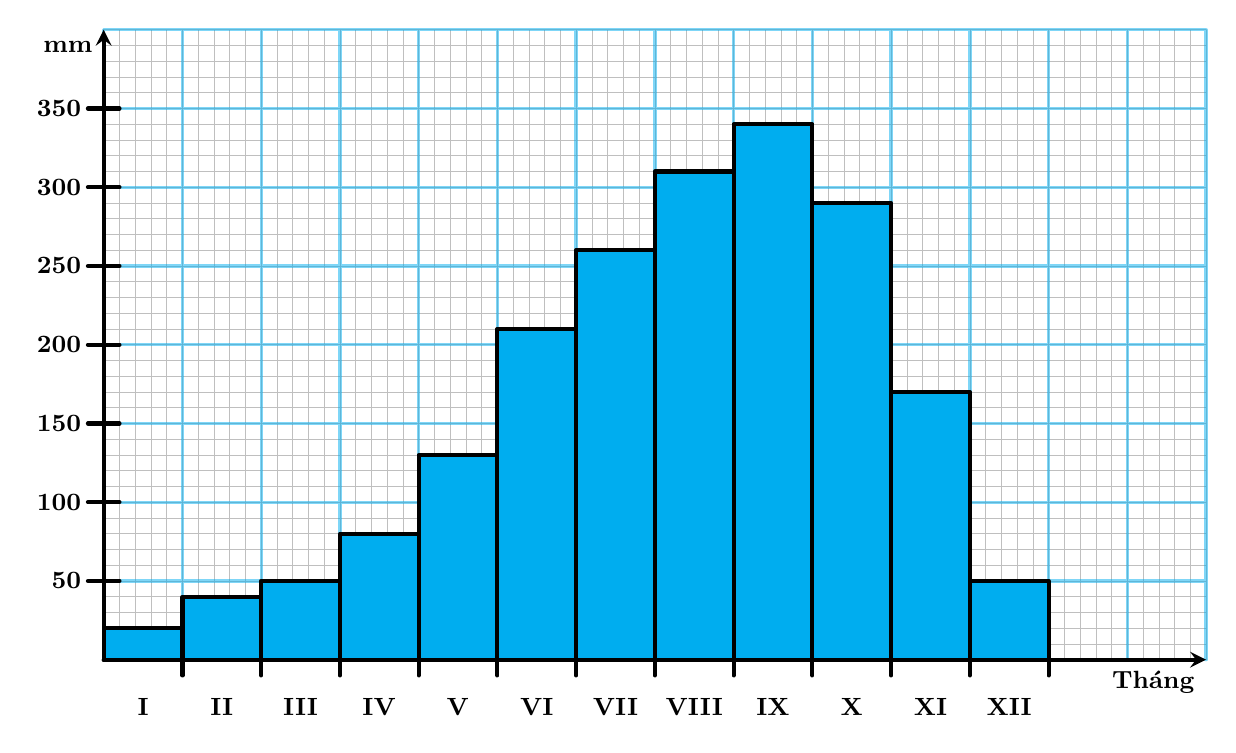
\begin{tikzpicture}[>=stealth,line width=1.5pt,line join=round,line cap=round,x=2cm,y=2cm,font=\small,scale=.5]
		\draw[step=0.2,gray,very thin,opacity=0.5] (0,0) grid (14,8);
		\draw[step=1,cyan,very thick,opacity=0.5] (0,0) grid (14,8);
		\draw[->] (0,0)--(14,0)node[below left]{\textbf{Tháng}};
		\draw[->] (0,0)--(0,8)node[below left]{\textbf{mm}};
		\def \a{0.2}
		\draw[fill=cyan] (0,0) rectangle (1,2*\a)
		(1,0) rectangle (2,4*\a)
		(2,0) rectangle (3,5*\a)
		(3,0) rectangle (4,8*\a)
		(4,0) rectangle (5,13*\a)
		(5,0) rectangle (6,21*\a)
		(6,0) rectangle (7,26*\a)
		(7,0) rectangle (8,31*\a)
		(8,0) rectangle (9,34*\a)
		(9,0) rectangle (10,29*\a)
		(10,0) rectangle (11,17*\a)
		(11,0) rectangle (12,5*\a);
		\foreach \x in {1,2,3,...,12} {
			\draw (\x,0) -- (\x,-0.2);
		};
		\foreach \x in {1,2,3,...,7} {
			\draw (-0.2,\x) -- (0.2,\x);
		};
		\foreach \x/\luongmua in {1/50, 2/100, 3/150, 4/200, 5/250, 6/300, 7/350} {
			\draw (0,\x) node[ label=left:\textbf{{\luongmua}}] {};
		}
		\foreach \x/\thang in {1/I, 2/II, 3/III, 4/IV, 5/V, 6/VI, 7/VII, 8/VIII, 9/IX, 10/X, 11/XI, 12/XII} {
			\draw (\x-0.5,-0.2) node[ label=below:\textbf{{\thang}}] {};
		}
		\end{tikzpicture}
		
		\textit{Hình 3.1. Biểu đồ lượng mưa ở thành phố $A$}
	\end{center}
	Xác định khoảng tứ phân vị của mẫu số liệu (làm tròn kết quả đến hàng đơn vị).
	
	\shortans{208}
	\loigiai{
				Bảng số liệu về lượng mưa của thành phố $A$:
			\begin{center}
				\begin{tabular}{|c|c|c|}
					\hline Lượng mưa (mm)  & Tần số  & Tần số tích luỹ \\
					\hline$[0 ; 50)$ & $2$ & $2$ \\
					\hline$[50 ; 100)$ & $3$ & $5$ \\
					\hline$[100 ; 150)$ & $1$ & $6$ \\
					\hline$[150 ; 200)$ & $1$ & $7$ \\
					\hline$[200 ; 250)$ & $1$ & $8$ \\
					\hline$[250 ; 300)$ & $2$ & $10$ \\
					\hline$[300 ; 350)$ & $2$ & $12$ \\
					\hline
				\end{tabular}	
			\end{center}
			Ta có
			$N=12$ nên  $\dfrac{N}{4}=3 ; \dfrac{3 N}{4}=9$.\\
			Nhóm chứa $Q_1$ là $[50 ; 100)$.
			$$Q_1=50+\dfrac{3-2}{3} \cdot 50 \approx 67.$$
			Nhóm chứa $Q_3$ là $[250 ; 300)$.
			$$Q_3=250+\dfrac{9-8}{2} \cdot 50=275.$$
			Vậy $\Delta_Q=275-67=208$.}
\end{bt}

\begin{bt}%[2D3V2-2]
% nguon: Archive/2025-Sangtac/Khoi12/Data/2-KNTT/KNTT_2-OTHK1_De01.tex #4741

	Chiều dài của 40 bé trai sơ sinh 12 ngày tuổi chọn ngẫu nhiên ở một bệnh viện được nhà nghiên cứu thống kê trong \textit{Bảng 3.17} dưới đây:
	\begin{center}
		\textit{Bảng 3.17. Chiều dài của 40 bé trai sơ sinh}\\
		\begin{tabular}{|l|c|c|c|c|c|c|}
			\hline \textbf{Chiều dài (cm)} & {$[44 ; 46)$} & {$[46 ; 48)$} & {$[48 ; 50)$} & {$[50 ; 52)$} & {$[52 ; 54)$} & {$[54 ; 56)$} \\
			\hline\textbf{Số trẻ }& 3 & 3 & 10 & 15 & 7 & 2 \\
			\hline
		\end{tabular}
	\end{center}
	Tìm độ lệch chuẩn của chiều dài nhóm 40 bé trai sơ sinh (làm tròn kết quả đến hàng phần nghìn).
	
	\shortans{2{,}43}
	\loigiai{
		Bổ sung thêm các giá trị đại diện vào bảng, ta lập được bảng sau:
		\begin{center}
			\textit{Chiều dài của 40 bé trai sơ sinh (đơn vị: cm)}\\
			\begin{tabular}{|c|c|c|}
				\hline \textbf{Nhóm} & $\boldsymbol{c}_{\boldsymbol{i}}$ & $\boldsymbol{n}_{\boldsymbol{i}}$ \\
				\hline$[44 ; 46)$ & 45 & 3 \\
				\hline$[46 ; 48)$ & 47 & 3 \\
				\hline$[48 ; 50)$ & 49 & 10 \\
				\hline$[50 ; 52)$ & 51 & 15 \\
				\hline$[52 ; 54)$ & 53 & 7 \\
				\hline$[54 ; 56)$ & 55 & 2 \\
				\hline & & $N=40$ \\
				\hline
			\end{tabular}
		\end{center}
		Từ mẫu số liệu đã cho, ta tính được số trung bình là:
		$$
		\overline{x}=\dfrac{3\cdot45+3\cdot47+10\cdot49+15\cdot51+7\cdot53+2\cdot55}{40}=\frac{2012}{40}=50{,}3
		$$
		$\overline{x}$ không phải là số nguyên nên ta chọn công thức (*) để tính phương sai:
		$$
		\overline{x^{2}}=\frac{3\cdot45^{2}+3\cdot47^{2}+10\cdot49^{2}+15\cdot51^{2}+7\cdot53^{2}+2\cdot55^{2}}{40}=2536.
		$$
		Do đó $s^{2}=\overline{x^{2}}-(\overline{x})^{2}=2536-50{,}3^{2}=2536-2530{,}09=5{,}91$.\\
		Vậy mẫu số liệu về chiều dài của 40 trẻ sơ sinh có độ lệch chuẩn là $s=\sqrt{5{,}91} \approx 2{,}43$.
	}
\end{bt}

\begin{ex}%[2D3H1-4]
% nguon: Archive/2025-Sangtac/Khoi12/Data/2-KNTT/KNTT_2-OTHK1_De04.tex #4744
%[Võ Thanh Hiệp]
	Thống kê mẫu số liệu ghép nhóm về cân nặng (đơn vị: kilôgam) của các học sinh lớp 12A và lớp 12B ở một trường trung học phổ thông như sau:
	\begin{center}
		\begin{tabular}{|c|c|c|c|c|c|c|c|c|}
			\hline
			\textbf{Số cân nặng} & $[45;50)$ & $[50; 55)$ & $[55;60)$ & $[60;65)$ &  $[65;70)$& $[70;75)$ &$[75;80)$ \\
			\hline
			\textbf{Số học sinh lớp 12A} & $4$ & $8$ & $12$ & $9$ & $ 4$& $ 2$& $1$ \\
			\hline
			\textbf{Số học sinh lớp 12B} & $5$ & $6$ & $8$ & $9$ & $6$& $3$&$ 0$\\
			\hline
		\end{tabular}
	\end{center}
	\choiceTF
	{\True Mốt của mẫu số liệu của học sinh lớp 12A khoảng $57{,}86$}
	{Khoảng biến thiên của mẫu số liệu ghép nhóm về cân nặng của các bạn học sinh lớp 12B là $35$ (kg)}
	{\True Giá trị trung bình cân nặng của học sinh lớp 12A  lớn hơn lớp 12B }
	{\True Một học sinh lớp 12A có cân nặng $78$ kg là giá trị ngoại lệ}
	\loigiai{
		\begin{itemchoice}
			\itemch {\bf Đúng.}\\
			Nhóm $[55;60)$ của lớp 12A có tần số  cao nhất là $12$ nên nhóm $[55;60)$ chứa mốt.\\
			Do đó mốt của mẫu số liệu ghép nhóm lớp 12A khoảng\\
			$$M_{o}=u_{m}+\dfrac{n_{m}-n_{m-1}}{\left(n_{m}-n_{m-1}\right)+\left(n_{m}-n_{m+1}\right)} \cdot\left(u_{m+1}-u_{m}\right)= 55 + \dfrac{4}{4+3}\cdot 5 \approx 57{,}86.$$
			\itemch {\bf Sai.}\\
				Vì khoảng biến thiên của mẫu số liệu lớp 12B là $75 - 45 =30$ (kg).
			\itemch {\bf Đúng.}
			\begin{center}
				\begin{tabular}{|c|c|c|c|c|c|c|c|c|}
					\hline
					\textbf{Số cân nặng} & $[45;50)$ & $[50; 55)$ & $[55;60)$ & $[60;65)$ &  $[65;70)$& $[70;75)$ &$[75;80)$ \\
					\hline
					\textbf{Số học sinh lớp 12A} & $4$ & $8$ & $12$ & $9$ & $ 4$& $ 2$& $1$ \\
					\hline
					\textbf{Số học sinh lớp 12B} & $5$ & $6$ & $8$ & $9$ & $6$& $4$&$ 0$\\
					\hline
					\textbf{Giá trị đại diện} & $47{,}5$ &$52{,}5$ & $57{,}5$ & $62{,}5$ & $67{,}5$& $72{,}5$&$77{,}5$\\
					\hline
				\end{tabular}
			\end{center}
			 Giá trị trung bình của lớp 12A bằng
			 $$\overline{x}=\dfrac{4\cdot 47{,}5+8\cdot 52{,}5+12\cdot 57{,}5+9\cdot 62{,}5+4\cdot 67{,}5+2\cdot 72{,}5+1\cdot 77{,}5}{4+8 +12+9+4+2+1}=\dfrac{1025}{16}.$$
			  Giá trị trung bình của lớp 12B bằng
			 $$\overline{x}=\dfrac{5\cdot 47{,}5+6\cdot 52{,}5+8\cdot 57{,}5+9\cdot 62{,}5+6\cdot 67{,}5+3\cdot 72{,}5+0\cdot 77{,}5}{5+6+8+9+6+3+0}=\dfrac{1135}{19}.$$
			 Vì $\dfrac{1025}{16}>\dfrac{1135}{19}$, nên giá trị trung bình cân nặng của học sinh lớp 12A  lớn hơn lớp 12B.
			\itemch {\bf Đúng.}\\
			Xét mẫu số liệu ghép nhóm lớp 12A.\\
			Cỡ mẫu $n= 4+8 +12+9+4+2+1= 40$.\\
			Tứ phân vị thứ nhất là $\dfrac{x_{10}+x_{11}}{2}$ thuộc nhóm $[50; 55)$, tứ phân vị thứ ba là $\dfrac{x_{30}+x_{31}}{2}$ thuộc nhóm $[60; 65)$. Suy ra\\
			$Q_1=50+\dfrac{\dfrac{40}{4}-4}{8}\cdot(55-50)= 53{,}75$,\\ $Q_3=60+\dfrac{\dfrac{3\cdot40}{4}-(4+8+12)}{9}\cdot(65-60)= \dfrac{190}{3}$.\\
			Khoảng tứ phân vị $\Delta_Q=Q_3-Q_1=\dfrac{190}{3}-53{,}75=\dfrac{115}{12}$.\\
			Ta có $Q_3+1{,}5\cdot\Delta_Q=\dfrac{190}{3}+1{,}5\cdot\dfrac{115}{12}=\dfrac{1865}{24}<78$. Vậy học sinh lớp 12A có cân nặng $78$ kg là giá trị ngoại lệ.
				\end{itemchoice}
	}
\end{ex}

\begin{ex}%[2D3H2-2]
% nguon: Archive/2025-Sangtac/Khoi12/Data/2-KNTT/KNTT_2-OTHK1_De04.tex #4745
%[Võ Thanh Hiệp] 
	\immini[thm]{
		Biểu đồ tần số tương đối hình quạt trong hình bên mô tả bảng phân bố tần suất ghép lớp của dữ liệu điểm kiểm tra môn Toán cuối học kỳ 1 của $40$ học sinh một lớp 12 trong kì kiểm tra học kỳ 1 môn Toán (thang điểm $10$).
	}
	{\begin{tikzpicture}[scale=0.7,>=stealth]
			\draw(0,0) circle (3cm);
			\draw[pattern=vertical lines, pattern color=black!50] (0,0) -- +(0:3) arc (0:36:3)--(0,0);
			
			\draw[pattern=north east lines, pattern color=green!30] (0,0) -- +(36:3) arc (36:108:3)--(0,0);
			
			\draw[pattern = horizontal lines, pattern color=red!30] (0,0) -- +(108:3) arc (108:216:3)--(0,0);  
			\draw[pattern=dots] (0,0) -- +(216:3) arc (216:306:3)--(0,0);
			\draw[pattern=vertical lines, pattern color=black!50] (3.5,1.5) rectangle (4,2) (5.25,1.75) node{\footnotesize $[5;6)$};
			\draw[pattern=north east lines, pattern color=black!50] (3.5,0.5) rectangle (4,1) (5.25,0.75) node{\footnotesize $[6;7)$};
			\draw[pattern = horizontal lines, pattern color=red!30] (3.5,-0.5) rectangle (4,0) (5.25,-0.25) node{\footnotesize $[7;8)$};
			\draw[pattern=dots] (3.5,-1.5) rectangle (4,-1) (5.25,-1.25) node{\footnotesize $[8;9)$};
			\draw (3.5,-2.5) rectangle (4,-2) (5.25,-2.25) node{\footnotesize $[9;10]$};
			\fill[white] 
			(1.75,.5) circle(0.5) node[black]{\footnotesize $10\%$}
			(.75,1.5) circle(0.5) node[black]{\footnotesize $20\%$}
			(-1.5,0.5) circle(0.5) node[black]{\footnotesize $30\%$ }
			(0,-1.5)circle(0.5) node[black]{\footnotesize $25\%$ }  
			(1.65,-0.65)circle(0.5) node[black]{\footnotesize $15\%$};
	\end{tikzpicture}}
	\choiceTF
	{\True Tần số của các giá trị đại diện $6{,}5$, $6{,}5$; $7{,}5$; $8{,}5$; $9{,}5$ của các lớp ghép nhóm lần lượt là $4$; $8$; $12$; $10$; $6$}
	{Điểm trung bình kiểm tra  môn Toán của lớp 12 đó là $\overline{x}=7{,}75$}
	{Khoảng tứ phân vị của bảng số liệu là $\Delta_Q=1{,}9$}
	{\True Độ lệch chuẩn của mẫu số liệu xấp xỉ $1{,}19$}
	\loigiai{
		\begin{itemchoice}
			\itemch {\bf Đúng.} Ta có bảng phân bố tần số, tần suất như sau
			\begin{center}
				\begin{tabular}{|c|c|c|c|c|c|c|}
					\hline 
					\bf Lớp &$[5;6)$&$[6;7)$ &$[7;8)$&$[8;9)$&$ [9;10]$& Cộng\\ 
					\hline
					\bf Giá trị đại diện &$5{,}5$& $6{,}5$&$7{,}5$&$8{,}5$&$9{,}5$&\\
					\hline
					\bf Tần số & $4$ & $8$ & $12$ & $10$ & $6$ &$n=40$\\
					\hline
					\bf Tần suất (\%) & $10$ &$20$&$30$&$25$&$15$&$100$ (\%)\\
					\hline
				\end{tabular}
			\end{center}
			Tần số của các giá trị đại diện $6{,}5$; $7{,}5$; $8{,}5$; $9{,}5$ của các lớp ghép nhóm lần lượt là $4$, $8$; $12$; $10$; $6$.
			\itemch {\bf Sai.}\\
			 Điểm thi trung bình môn Toán của lớp 12B19 là
			$$\overline{x}= \dfrac{5{,}5\cdot4 +6{,}5\cdot8+7{,}5\cdot12+8{,}5\cdot10+9{,}5\cdot6}{40}=7{,}65.$$
			\itemch {\bf Sai.}\\
			Cỡ mẫu $n=40$.\\
			Gọi $x_1 ; x_2 ; \ldots ; x_{40}$ là mẫu số liệu gốc của điểm kiểm tra học kì của $40$ học sinh được xếp theo thứ tự không giảm.
			Ta có\\ $x_1,\ldots, x_{10} \in[6;7)$; $x_{11}, \ldots, x_{20} \in[7;8)$; $x_{21}, \ldots, x_{30} \in[8;9)$; $x_{31}, \ldots, x_{40} \in[9;10]$.\\
			Tứ phân vị thứ nhất của mẫu số liệu gốc là $\dfrac{1}{2}\left(x_{10}+x_{11}\right) \in[6;7)$. Do đó, tứ phân vị thứ nhất của mẫu số liệu ghép nhóm là
			$$
			Q_1=6+\dfrac{\dfrac{40}{4}-4}{8} \cdot(7-6)=6{,}75.
			$$			
			Tứ phân vị thứ ba của mẫu số liệu gốc là $\dfrac{1}{2}\left(x_{30}+x_{31}\right) \in[8;9)$. Do đó, tứ phân vị thứ ba của mẫu số liệu ghép nhóm là
			$$
			Q_3=8+\dfrac{\dfrac{3\cdot40}{4}-(4+8+12)}{10} \cdot(9-8)=8{,}6.
			$$			
			Vậy khoảng tứ phân vị của mẫu số liệu ghép nhóm là
			$$
			\Delta_Q=8{,}6-6{,}75=1{,}85.
			$$
			\itemch {\bf Đúng.} \\
			Phương sai của mẫu số liệu được được tính theo công thức
			$$S^2=\dfrac{5{,}5^2\cdot4 +6{,}5^2\cdot8+7{,}5^2\cdot12+8{,}5^2\cdot10+9{,}5^2\cdot6}{40}-7{,}65^2=\dfrac{571}{400}.$$
			Suy ra độ lệch chuẩn của mẫu số liệu là $S=\sqrt{S^2}=\dfrac{\sqrt{571}}{20}\approx 1{,}19$.
		\end{itemchoice}
	}
\end{ex}

\begin{bt}%[2D3V1-4]
% nguon: Archive/2025-Sangtac/Khoi12/Data/2-KNTT/KNTT_2-OTHK1_De04.tex #4750
%[Võ Thanh Hiệp]
Thời gian (đơn vị: giây) chạy $100$ m của đội điền kinh gồm $20$ học sinh được cho bởi biểu đồ tần suất như sau:
	\begin{center}
		\begin{tikzpicture}[scale=1,>=stealth]
			\pgfplotsset{compat=1.16}
			\begin{axis}[
				ybar,
				bar width=1,
				ymin=0,
				ymax=.5,
				enlarge x limits={abs=2},
				xtick=data,
				height=7cm, width=9.6cm,
				point meta=y*100,
				nodes near coords={\pgfmathprintnumber\pgfplotspointmeta\%},
				nodes near coords style={/pgf/number format/precision=3,
					/pgf/number format/fixed},
				xticklabels={,,,,},
				yticklabel={\pgfmathparse{\tick*100}\pgfmathprintnumber{\pgfmathresult}},
				tickwidth=0,
				ymajorgrids,
				axis y line*=left,
				axis x line*=left,
				]
				\addplot[fill=black!20] table[x expr=\coordindex,y index=0,row sep=\\] {0.05\\0.1\\0.4\\0.3\\0.15\\};
			\end{axis}
			\draw[->,line width=1 pt] (0:0)--(0:8.5) node[below right,pos=.9,rectangle,minimum width=3.5cm,minimum height=1cm,text width=3.5cm] {Giây};
			\draw[->,line width=1 pt] (0:0)--(90:7) node[above left,pos=.8,rectangle,minimum width=2.5cm,minimum height=1cm,text width=2.5cm] {Tần suất (\%)};
			\foreach \x/\y in {1.5/11,2.5/12,3.5/13,4.5/14,5.5/15,6.5/16}
			\draw[thin] (\x,1pt)--(\x,-1pt) node [below] {$\y$};
		\end{tikzpicture}		
	\end{center}
	Giáo  viên muốn chọn đội tuyển đi thi đấu giải gồm $5$ học sinh có thành tích cao nhất trong đội điền kinh nói trên. Hỏi giáo viên chọn những học sinh có thành tích tối đa là bao nhiêu giây (kết quả làm tròn đến hàng phần mười)? 
	
	\shortans{13{,}3}
	\loigiai{
		Ta có bảng tần số, tần suất ghép nhóm như sau
		\begin{center}
			\begin{tabular}{|m{3cm}|m{2cm}|m{2cm}|m{2cm}|m{2cm}|m{2cm}| m{2cm}|}
				\hline 
				\centering\arraybackslash Nhóm & 
				\centering\arraybackslash$\left[11;2\right)$ & 
				\centering\arraybackslash$\left[12;13\right)$ & 
				\centering\arraybackslash$\left[13;14\right)$ & 
				\centering\arraybackslash$\left[14;15\right)$ & 
				\centering\arraybackslash$\left[15;16\right)$ &
				\centering\arraybackslash  Cộng\\ 
				\hline  
				\centering\arraybackslash Tần số & 
				\centering\arraybackslash$1$ & 
				\centering\arraybackslash$2$ & 
				\centering\arraybackslash$8$ & 
				\centering\arraybackslash$6$ & 
				\centering\arraybackslash$3$ &
				\centering\arraybackslash  20\\ 
				\hline 
				\centering\arraybackslash Tần suất \% & 
				\centering\arraybackslash$5$ & 
				\centering\arraybackslash$10$ & 
				\centering\arraybackslash$40$ & 
				\centering\arraybackslash$30$ & 
				\centering\arraybackslash$15$ &
				\centering\arraybackslash  $100\%$\\ 
				\hline 
			\end{tabular}
		\end{center}
		Gọi $x_1 ; x_2 ; \ldots ; x_{20}$ là thành tích chạy của mẫu số liệu gốc của của $20$ học sinh được xếp theo thứ tự không giảm.\\
		Để chọn được $5$ học sinh có thành tích cao nhất trong đội điền kinh thì số học sinh được chọn thuộc phần bên trái của tứ phân vị thứ nhất.\\
		Tứ phân vị thứ nhất của mẫu số liệu gốc là $\dfrac{x_{5}+x_{6}}{2}\in \left[13;14\right)$.\\ 
		Do đó, tứ phân vị thứ nhất của mẫu số liệu ghép nhóm là
		$$Q_1=13+\dfrac{\dfrac{20}{4}-(1+2)}{8}\left(14-3\right)=\dfrac{53}{4}\approx 13{,}3.$$
		Vậy những học sinh có thành tích tối đa là $13{,}3$ giây thì được chọn đi thi đấu giải.
		}
\end{bt}

\begin{bt}%[2D3V2-2]
% nguon: Archive/2025-Sangtac/Khoi12/Data/2-KNTT/KNTT_2-OTHK1_De04.tex #4751
%[Võ Thanh Hiệp]
 	Thống kê chiều cao (đơn vị: cm) của 30 học sinh lớp 1 của một trường tiểu học được ghi lại ở biểu đồ sau:
 	\begin{center}
 		\begin{tikzpicture}[scale=1,>=stealth]
 			\begin{axis}[
 				%title={\bf Biểu đồ theo tần số chiều cao của 30 học sinh},
 				ybar,
 				width=10cm,
 				enlargelimits=.09,
 				legend style={at={(0.4,-0.25)},
 					anchor=north,legend columns=-1},
 				bar width=12mm, y=6mm,
 				symbolic x coords={[115;120), [120;125), [125;130), [130;135), [135;140)},
 				tickwidth=0,
 				ymajorgrids,
 				axis y line*=left,
 				axis x line*=left,
 				nodes near coords,
 				]
 			\addplot[fill=black!20] coordinates {([115;120),4) ([120;125),8) ([125;130),10) ([130;135),6) ([135;140),2)};
 			\end{axis}
 			\draw[->,line width=1 pt] (0:0)node[left]{$0$}--(0:10) node[below right,pos=.9,rectangle,minimum width=3cm,minimum height=1cm,text width=3cm] {Chiều cao (cm)};
 			\draw[->,line width=1 pt] (0:0)--(90:6) node[above left,pos=.9,rectangle,minimum width=1.5cm,minimum height=1cm,text width=1.5cm] {Số học sinh};
 		\end{tikzpicture}
 	\end{center}
 	Phương sai của mẫu số liệu ghép nhóm trên (làm tròn đến hàng phần trăm) là
 	
 	\shortans{5{,}54}
  	\loigiai{
 		Bảng số liệu ghi theo giá trị đại diện là
 		\begin{center}
 			\begin{tabular}{
 					| m{3cm}
 					| m{2cm}
 					| m{2cm}
 					| m{2cm}
 					| m{2cm}
 					| m{2cm}|
 				}
 				\hline
 				\centering\arraybackslash Chiều cao (cm) & 
 				\centering\arraybackslash$[115; 120)$ & 
 				\centering\arraybackslash$120; 125)$ & 
 				\centering\arraybackslash$[125; 130)$ & 
 				\centering\arraybackslash$[130; 135)$ & 
 				\centering\arraybackslash$[135; 140)$ \\
 				\hline
 				\centering\arraybackslash Giá trị đại diện & 
 				\centering\arraybackslash $117{,}5$ & 
 				\centering\arraybackslash $122{,}5$ & 
 				\centering\arraybackslash $127{,}5$ & 
 				\centering\arraybackslash $132{,}5$ & 
 				\centering\arraybackslash $137{,}5$ \\
 				\hline
 				\centering\arraybackslash Số học sinh & 
 				\centering\arraybackslash$4$ & 
 				\centering\arraybackslash$8$ & 
 				\centering\arraybackslash$10$ & 
 				\centering\arraybackslash$6$ & 
 				\centering\arraybackslash$2$ \\
 				\hline
 			\end{tabular}
 		\end{center}
 		Cỡ mẫu $n= 4 + 8 + 10 + 6 + 2 = 30$.\\
 		Giá trị trung bình của mẫu số liệu ghép nhóm là
 		$$\overline{x}=\dfrac{1}{30}(4\cdot117{,}5+8\cdot 122{,}5+10\cdot 127{,}5+6\cdot 132{,}5+2\cdot 137{,}5)=126{,}5.$$
 		Phương sai của mẫu số liệu ghép nhóm là
 		$$S^2=\dfrac{1}{30}(4\cdot117{,}5^2+8\cdot 122{,}5^2+10\cdot 127{,}5^2+6\cdot 132{,}5^2+2\cdot 137{,}5^2)-126{,}5^2=\dfrac{92}{3}.$$
 		Phương sai của mẫu số liệu ghép nhóm trên (làm tròn đến hàng phần trăm) là\\ $S=\sqrt{S^2}=\sqrt{\dfrac{92}{3}}\approx 5{,}54$.
 	}
 \end{bt}

\begin{ex}%[2D3H1-4]
% nguon: Archive/2025-Sangtac/Khoi12/Data/2-KNTT/KNTT_2-OTHK1_De05.tex #4754
%[Thầy Tú TLH]%câu3
	Cho bảng mẫu số liệu ghép nhóm về điểm môn Toán của hai lớp 12A và 12B được cho như sau:\\
	\centerline{\begin{tabular}{|c|c|c|c|c|c|c|c|}
			\hline
			Khoảng điểm &$[3;4)$ & $[4;5)$ & $[5;6)$ & $[6;7)$ & $[7;8)$ & $[8;9)$ & $[9;10)$\\
			\hline
			Số học sinh lớp 12A & $0$ & $1$ & $3$ & $6$ & $17$ & $7$ & $2$\\
			\hline
			Số học sinh lớp 12B & $1$ & $3$ & $13$ & $11$ & $5$ & $3$ & $0$\\
			\hline
	\end{tabular}}\\
	\choiceTF
	{Khoảng biến thiên cho điểm môn Toán của lớp 12A là $7$}
	{\True Khoảng biến thiên cho điểm môn Toán của lớp 12B là $6$}
	{\True Nhóm chứa tứ phân vị thứ nhất của lớp 12A là nhóm $[6;7)$}
	{Nhóm chứa tứ phân vị thứ ba của lớp 12B là nhóm $[7;8)$}
	\loigiai{
		\begin{itemchoice}
			\itemch \textbf{Sai}.\\
			Khoảng biến thiên của điểm môn Toán của lớp 12A là $R_1=10-4=6$.
			\itemch \textbf{Đúng}.\\
			Khoảng biến thiên cho điểm môn Toán của lớp 12B là $R_2=9-3=6$.
			\itemch \textbf{Đúng}.\\
			Ta có $n=1+3+13+11+5+3=36$.\\
			Gọi $x_1$, $\ldots$, $x_{36}$ là điểm của $36$ học sinh lớp 12A được sắp xếp theo thứ tự không giảm.\\
			Tứ phân vị thứ nhất của mẫu số liệu gốc là $x_9$ nên nhóm chứa phân vị thứ nhất là nhóm $[6;7)$.
			\itemch \textbf{Sai}.\\
			Tứ phân vị thứ ba của mẫu số liệu gốc là $x_{27}$ nên nhóm chứa phân vị thứ ba là nhóm $[6;7)$.
		\end{itemchoice}
	}
\end{ex}

\begin{ex}%[2D3V1-4]
% nguon: Archive/2025-Sangtac/Khoi12/Data/2-KNTT/KNTT_2-OTHK1_De05.tex #4755
%[Thầy Tú TLH] %câu4
Bác tài xế A và bác tài xế B thống kê lại độ dài quãng đường (đơn vị: km) mà hai bác đã lái xe mỗi ngày trong một tháng ở bảng sau:
\begin{center}
	\begin{tabular}{|c|c|c|c|c|c|c|}
		\hline
		Độ dài quãng đường (km) & $[50;100)$ & $[100;150)$ & $[150;200)$ & $[200;250)$ & $[250;300)$ &\\
		\hline
		Số ngày bác tài A lái xe & $5$ & $10$ & $9$ & $4$ & $2$ &$n_A=30$ \\
		\hline
		Số ngày bác tài B lái xe & $4$ & $8$ & $12$ & $6$ & $0$ &$n_B=30$\\
		\hline
	\end{tabular}
\end{center}
\choiceTF
{Khoảng biến thiên về độ dài quãng đường đi mỗi ngày của bác tài A và bác tài B ở mẫu số liệu trên bằng nhau}
{Tứ phân vị thứ nhất của mẫu số liệu về độ dài quãng đường mỗi ngày của bác tài A lớn hơn tứ phân vị thứ nhất của mẫu số liệu về độ dài quãng đường mỗi ngày của bác tài B}
{\True Tứ phân vị thứ ba của mẫu số liệu về quãng đường mỗi ngày của bác tài B thuộc nhóm $[150;200)$}
{\True Theo khoảng biến thiên thì độ dài quãng đường mỗi ngày bác tài A lái xe phân tán hơn độ dài quãng đường mỗi ngày bác tài B lái xe}
\loigiai{
	\begin{itemchoice}
		\itemch {\bf Sai}. \\
		Khoảng biến thiên về độ dài quãng đường đi của bác tài A là $300 - 50 = 250$. \\
		Khoảng biến thiên về độ dài quãng đường đi của bác tài B là $250 - 50 = 200$.
		\itemch {\bf Sai}. \\
		Tứ phân vị thứ nhất của mẫu số liệu về độ dài quãng đường mỗi ngày của bác tài A là
		\[Q_1 = 100 + \dfrac{\dfrac{30}{4} -5}{10}\cdot 50 = 112{,}5.\]
		Tứ phân vị thứ nhất của mẫu số liệu về độ dài quãng đường mỗi ngày của bác tài B là
		\[Q_1 = 100 + \dfrac{\dfrac{30}{4} - 4}{8}\cdot 50 = 121{,}875.\]
		\itemch \textbf{Đúng}. \\
		Tứ phân vị thứ ba của mẫu số liệu gốc về quãng đường mỗi ngày của bác tài B là $x_{23}$ nên thuộc nhóm $[150;200)$.
		\itemch {\bf Đúng}. \\
		Vì khoảng biến thiên về độ dài quãng đường đi của bác tài A lớn hơn khoảng biến thiên về độ dài quãng đường đi của bác tài B nên mức độ phân tán về độ dài quãng đường của bác tài A nhiều hơn mức độ phân tán về độ dài quãng đường của bác tài B.
\end{itemchoice}
}
\end{ex}

\begin{bt}%[2D3H1-3]
% nguon: Archive/2025-Sangtac/Khoi12/Data/2-KNTT/KNTT_2-OTHK1_De05.tex #4758
%[Thầy Tú TLH]%câu4
	Thời gian luyện tập trong một ngày (tính theo giờ) của một số vận động viên được ghi lại ở bảng sau:
	\begin{center}
		\begin{tabular}{|c|c|c|c|c|c|}
			\hline Thời gian luyện tập (giờ) & $[0;2)$ & $[2;4)$ & $[4;6)$ & $[6;8)$ & $[8;10)$ \\ 
			\hline Số vận động viên & $3$ & $8$ & $12$ & $12$ & $4$ \\ 
			\hline 
		\end{tabular} 
	\end{center}
	Hãy xác định khoảng tứ phân vị của mẫu số liệu đã cho (làm tròn đến hàng phần trăm).\par
	\shortans[]{3{,}35}
	\loigiai{
		Số vận động viên được khảo sát là $ n=3+8+12+12+4=39$.\\
		Gọi $ x_1 $, $ x_2 $, \ldots, $ x_{39} $ là thời gian luyện tập của $ 39 $ vận động viên được xếp theo thứ tự không giảm. \\
		Ta có\\
		$ x_1, x_2, x_3 \in [0;2) $; 
		$ x_4, \ldots, x_{11}\in [2;4) $;
		$ x_{12}, \ldots, x_{23}\in [4;6) $; 
		$ x_{24}, \ldots, x_{35}\in [6;8) $; 
		$ x_{36},\ldots , x_{39}\in [8;10) $.
		\begin{itemize}
			\item Tứ phân vị thứ nhất của mẫu số liệu gốc là $ x_{10} $ thuộc nhóm $[2;4)$;
			\item Tứ phân vị thứ ba của mẫu số liệu gốc là $ x_{30} $ thuộc nhóm $ [6;8) $.
		\end{itemize}
		Tứ phân vị thứ nhất của mẫu số liệu ghép nhóm là
		\begin{align*} 
			Q_1=2+\dfrac{\dfrac{1\cdot 39}{4}-3}{8}\cdot(4-2)=\dfrac{59}{16}.
		\end{align*} 
		Tứ phân vị thứ ba của mẫu số liệu ghép nhóm là 
		\begin{align*} 
			Q_3=6+\dfrac{\dfrac{3\cdot 39}{4}-(3+8+12)}{12}\cdot(8-6)=\dfrac{169}{24}.
		\end{align*} 
		Khoảng tứ phân vị $\Delta Q=Q_3-Q_1=\dfrac{161}{48}\approx 3{,}35$.
	}
\end{bt}

\begin{bt}%[2D3V2-2]
% nguon: Archive/2025-Sangtac/Khoi12/Data/2-KNTT/KNTT_2-OTHK1_De05.tex #4760
%[Thầy Tú TLH]%câu6
	Tốc độ của $20$ xe hơi khi đi qua một trạm kiểm tra tốc độ (đơn vị: km/h) được thống kê lại như sau:
	\begin{center}
		\begin{tabular}{cccccccccc}
			$42$ & $43{,}4$ & $43{,}4$ & $46{,}5$ & $46{,}7$ & $46{,}8$ & $47{,}5$ & $47{,}7$ & $48{,}1$ & $48{,}4$ \\ 
			$50{,}8$ & $52{,}1$ & $52{,}7$ &$ 53{,}9$ & $54{,}8$ & $55{,}6$ & $57{,}5$ & $59{,}6$ & $60{,}3$ & $61{,}1$
		\end{tabular} 
	\end{center}
	Tính độ lệch chuẩn (làm tròn kết quả đến hàng phần trăm) của mẫu số liệu ghép nhóm với các lớp ghép nhóm $[42;46)$; $[46;50)$; $[50;54)$; $[54;58)$; $[58;62)$.
	
	\shortans[]{5{,}15}
	\loigiai{
		\begin{center}
			\begin{tabular}{|c|c|c|c|c|c|}
				\hline Tốc độ (km/h) & $[42;46)$ & $[46;50)$ & $[50;54)$ & $[54;58)$ & $[58;62)$ \\
				\hline Giá trị đại diện & $44$ & $48$ & $52$ & $56$ & $60$ \\
				\hline Số xe & $3$ & $7$ & $4$ & $3$ & $3$ \\
				\hline
			\end{tabular}
		\end{center}
		Số trung bình của mẫu số liệu ghép nhóm là
		\[\overline{x}=\dfrac{3\cdot 44 + 7\cdot 48 + 4\cdot 52 + 3\cdot 56 + 3\cdot 60}{20}=51{,}2.\]
		Phương sai của mẫu số liệu ghép nhóm là
		\[s^2 = \dfrac{1}{20}\left(3\cdot 44^2 + 7\cdot 48^2 + 4\cdot 52^2 + 3\cdot 56^2 + 3\cdot 60^2 \right) - 51{,}2^2 = 26{,}56.\]
		Độ lệch chuẩn của mẫu số liệu ghép nhóm là $s = \sqrt{26{,}56} \approx 5{,}15$. 
	}
\end{bt}

\begin{ex}%[2D3H1-3]
% nguon: Archive/2025-Sangtac/Khoi12/Data/2-KNTT/KNTT_2-OTHK1_De06.tex #4763
%[2-D3B3-SO-8-2425]%[VN-MT-7, Lại Thị Hảo]
	Một vườn thú ghi lại tuổi thọ (đơn vị: năm) của $20$ con hổ và thu được kết quả như sau:
	\begin{center}
		\begin{tabular}{|c|c|c|c|c|c|}
			\hline
			Tuổi thọ & $[14; 15)$ & $[15; 16)$ & $[16; 17)$ & $[17; 18)$ & $[18; 19)$\\
			\hline
			Số con hổ & $1$ & $3$ & $8$ & $6$ & $2$ \\
			\hline
		\end{tabular}
	\end{center}
	\choiceTF
	{\True Khoảng biến thiên của mẫu số liệu ghép nhóm này là $5$}
	{\True Nhóm chứa tứ phân vị thứ nhất là $[16; 17)$}
	{Nhóm chứa tứ phân vị thứ ba là $[18; 19)$}
	{\True Tần số tích lũy của nhóm $[17; 18)$ là $18$}
	\loigiai{
		\begin{itemchoice}
			\itemch \textbf{Đúng}.\\
			Khoảng biến thiên $R=19-14=5$.
			\itemch \textbf{Đúng}.\\
			Cỡ mẫu là $1+3+8+6+2=20$.\\
			Gọi $x_1, x_2, \ldots, x_{20}$ là tuổi thọ của $20$ con hổ được sắp xếp theo thứ tự không giảm.\\
			Tứ phân vị thứ nhất của mẫu số liệu gốc là $\dfrac{x_5+x_6}{2} \in[16; 17)$ nên nhóm chứa tứ phân vị thứ nhất là $[16; 17)$.
			\itemch \textbf{Sai}.\\
			Tứ phân vị thứ ba của mẫu số liệu gốc là $\dfrac{x_{15}+x_{16}}{2} \in[17; 18)$. Do đó nhóm chứa tứ phân vị thứ ba là $[17; 18)$.
			\itemch \textbf{Đúng}.\\
			Tần số tích lũy của nhóm $[17; 18)$ là $1+3+8+6=18$.
		\end{itemchoice}
	}
\end{ex}

\begin{bt}%[2D3H2-2]
% nguon: Archive/2025-Sangtac/Khoi12/Data/2-KNTT/KNTT_2-OTHK1_De06.tex #4764
%[2-D3B3-SO-11-2425]%[VN-MT-7, Nguyen Huynh]
	Số người xem trong $60$ buổi chiếu phim của một rạp chiếu phim nhỏ.
	\begin{center}
		\begin{tabular}{|c|c|c|c|c|c|c|c|}
			\hline
			Lớp người xem & $[0; 10)$&$[10; 20)$&$[20; 30)$&$[30; 40)$&$[40; 50)$&$[50; 60]$&Cộng\\
			\hline
			Tần số & $5$&$9$&$11$&$15$&$12$&$8$&$60$\\
			\hline
		\end{tabular}
	\end{center}
	Hãy tính phương sai của mẫu số liệu ghép nhóm trên (kết quả được làm tròn đến hàng đơn vị). 
	
	\shortans{220}
	\loigiai{
		\begin{center}
			\begin{tabular}{|c|c|c|c|c|c|c|c|}
				\hline
				Lớp người xem & $[0; 10)$&$[10; 20)$&$[20; 30)$&$[30; 40)$&$[40; 50)$&$[50; 60]$&Cộng\\
				\hline
				Giá trị đại diện & $5$ & $15$ & $25$ & $35$ & $45$ & $55$ & \\
				\hline
				Tần số & $5$&$9$&$11$&$15$&$12$&$8$&$60$\\
				\hline
			\end{tabular}
		\end{center}
		Số trung bình của mẫu số liệu ghép nhóm là
		\begin{eqnarray*}
			\overline{x}&=&\dfrac{n_1c_1+n_2c_2+n_3c_3+n_4c_4+n_5c_5+n_6c_6}{n}\\
			&=&\dfrac{5 \cdot 5+9 \cdot 15+11 \cdot 25+15 \cdot 35+12 \cdot 45+8 \cdot 55}{60}\\
			&=&\dfrac{97}{3}\approx 32{,}3.
		\end{eqnarray*}
		\[s_x^2=\dfrac{5 \cdot 5^2+9 \cdot 15^2+11 \cdot 25^2+15 \cdot 35^2+12 \cdot 45^2+8 \cdot 55^2}{60}-\left(\dfrac{97}{3}\right)^2 \approx 220.\] 
	}
\end{bt}

\begin{ex}%[2D3H1-3]
% nguon: Archive/2025-Sangtac/Khoi12/Data/2-CD/CD_2-OTHK1_De02.tex #4772

Người ta đo đường kính của $61$ cây gỗ được trồng sau $12$ năm (đơn vị: cm), họ thu được bảng tần số ghép nhóm sau:
\begin{center}
\begin{tabular}{|l|c|c|c|c|c|}
\hline
Đường kính&$[20;25)$&$[25;30)$&$[30;35)$&$[35;40)$&$[40;45)$\\
\hline
Số cây&$4$&$12$&$26$&$13$&$6$\\
\hline
\end{tabular}
\end{center}
\choiceTF
{\True Số cây có đường kính từ $20$\,cm đến dưới $30$\,cm là $16$ cây}
{\True Khoảng biến thiên của mẫu số liệu ghép nhóm trên là $25$\,cm}
{\True Để chọn ra $50\%$ các cây gỗ có đường kính lớn nhất thì ta nên chọn các cây gỗ có đường kính từ $32{,}79$\,cm trở lên (làm tròn đến hàng phần trăm)}
{\True Khoảng tứ phân vị của mẫu số liệu ghép nhóm trên là $6{,}75$\,cm (làm tròn đến hàng phần trăm)}
\loigiai{
Bảng tần số ghép nhóm của mẫu số liệu trên như sau:
\begin{center}
\begin{tabular}{|l|c|c|c|c|c|}
\hline
Đường kính&$[20;25)$&$[25;30)$&$[30;35)$&$[35;40)$&$[40;45)$\\
\hline
Giá trị đại diện&$22,5$&$27,5$&$32,5$&$37,5$&$42,5$\\
\hline
Số cây&$4$&$12$&$26$&$13$&$6$\\
\hline
Tần số tích lũy&$4$&$16$&$42$&$55$&$61$\\
\hline
\end{tabular}
\end{center}
\begin{itemchoice}
\itemch {\bf Đúng}.\\
Số cây có đường kính từ $20$ cm đến dưới $30$ cm là $16$ cây.
\itemch {\bf Đúng}.\\
Khoảng biến thiên của mẫu số liệu là $45-20=25$.
\itemch {\bf Đúng}.\\
Số phần tử của mẫu là $n=4+12+26+13+6=61$.\\
Gọi $x_1$, $x_2$, $\ldots$, $x_{61}$ lần lượt là đường kính của cây theo thứ tự không giảm.\\
Tứ phân vị thứ hai của dãy số liệu là $x_{31}$ thuộc nhóm $[30;35)$ nên tứ phân vị thứ hai của mẫu số liệu là 
\[Q_2=30+\dfrac{\dfrac{61}{2}-16}{26}\cdot (35-30)=\dfrac{1\,705}{52}\approx 32{,}79.\]
Vậy để chọn ra $50\%$ các cây gỗ có đường kính lớn nhất thì ta nên chọn các cây gỗ có đường kính (làm tròn đến hàng phần trăm) từ $32{,}79$ cm trở lên.
\itemch {\bf Đúng}.\\
Tứ phân vị thứ nhất của dãy số liệu là $\dfrac{1}{2}(x_{15}+x_{16})$ thuộc nhóm $[25;30)$ nên tứ phân vị thứ nhất của mẫu số liệu là 
\[Q_1=25+\dfrac{\dfrac{61}{4}-4}{12}\cdot (30-25)=\dfrac{475}{16}\approx 29{,}69.\]
Tứ phân vị thứ ba của dãy số liệu là $\dfrac{1}{2}(x_{46}+x_{47})$ thuộc nhóm $[35;40)$ nên tứ phân vị thứ ba của mẫu số liệu là 
\[Q_3=35+\dfrac{\dfrac{3\cdot 61}{4}-42}{13}\cdot (40-35)=\dfrac{1\,895}{52}\approx 36{,}44.\]
Khoảng tứ phân vị của mẫu số liệu ghép nhóm trên là \[\Delta_Q=Q_3-Q_1=\dfrac{1\,895}{52}-\dfrac{475}{16}=\dfrac{1\,405}{208}\approx 6{,}75.\]
\end{itemchoice}
}
\end{ex}

\begin{bt}%[2D3V1-3]
% nguon: Archive/2025-Sangtac/Khoi12/Data/2-CD/CD_2-OTHK1_De02.tex #4778

	Biểu đồ dưới đây biểu diễn số lượt khách hàng đặt bàn qua hình thức trực tuyến mỗi ngày trong quý III năm $2024$ của một nhà hàng. Cột thứ nhất biểu diễn số ngày có từ $1$ đến dưới $6$ lượt đặt bàn; cột thứ hai biểu diễn số ngày có từ $6$ đến dưới $11$ lượt đặt bàn; \ldots
	\begin{center}
		\begin{tikzpicture}[scale=0.9,line cap=round,line join=round,font=\footnotesize,>=stealth]
			%\def\mau{{"orange","blue!50","orange","blue!50","orange","blue!50","orange","blue!50","orange","blue!50"}}
			\def\tg{{"1","6","11","16","21","26"}}
			\foreach \y[count=\i from 0] in {2.8,6,5,3.6,1}{
				\pgfmathsetmacro\giatri{int(round(5*\y))}
				%\pgfmathsetmacro\col{\mau[\i]}
				\draw[fill=blue!50] (1+2*\i,0) rectangle ++(1,\y)node[shift={(150:0.6)},scale=.8]{$\giatri$};
				\draw[dashed] (0,\y)--++(2*\i+1,0);
			}
			\draw[->] (0,0)--(0,7.5)node[above]{số ngày};
			\draw[->] (0,0)--(13,0)node[below]{Số lượt đặt bàn};
			\foreach \a in {1,2,...,6}{
				\pgfmathsetmacro\b{int(5*\a)}
				\fill[black] (0,\a)circle(.7pt)node[left,scale=.7]{$\b$};
			}
			\foreach \i in {0,1,2,3,4,5}{
				\pgfmathsetmacro\j{2*\i+1}
				\pgfmathsetmacro\gio{\tg[\i]}
				\fill (\j,0)node[below,scale=.8]{\gio};
			}
%			\fill[orange] (6,1) rectangle ++(.2,.2)node[right]{Bác Bình};
%			\fill[blue!50] (6,0.5) rectangle ++(.2,.2)node[right]{Bác An};
			\fill (6,8)node{\textbf{Số lượng khách hàng đặt bàn trực tuyến}};
		\end{tikzpicture}
	\end{center}
	Hãy tìm khoảng tứ phân vị của mẫu số liệu ghép nhóm cho bởi biểu đồ trên.
	
\shortans{8{,}5}
\loigiai{
	Từ biểu đồ đã cho, ta có có bảng thống kê sau:
	\begin{center}
		\begin{tabular}{|l|c|c|c|c|c|}
		\hline
		Số lượt đặt bàn & $[1; 6)$ & $[6; 11)$ & $[11; 16)$ & $[16; 21)$ & $[21; 26)$ \\
		\hline
		Số ngày & $14$ & $30$ & $25$ & $18$ & $5$ \\
		\hline
	\end{tabular}
	\end{center}
	Cỡ mẫu $n = 14 + 30 + 25 + 18 + 5 = 92$.\\
	Gọi $x_1; x_2; \ldots; x_{92}$ là mẫu số liệu gốc về số lượt khách đặt bàn qua hình thức trực tuyến mỗi ngày trong quý III năm $2022$ của một nhà hàng được xếp theo thứ tự không giảm. 
	Ta có
	\begin{center}
		\begin{tabular}{lll}
		$x_1;\ldots;x_{14}\in  [1; 6)$,&
		$x_{15};\ldots;x_{44}\in  [6; 11)$,&
		$x_{45};\ldots;x_{69}\in  [11; 16)$,\\
		$x_{70};\ldots;x_{87}\in  [16; 21)$,&
		$x_{88};\ldots;x_{92}\in  [21; 26)$.&
	\end{tabular}
	\end{center}
	Tứ phân vị thứ nhất của mẫu số liệu gốc là $\dfrac{x_{23}+x_{24}}{2}\in [6; 11)$. \\
	Do đó, tứ phân vị thứ nhất của mẫu số liệu ghép nhóm là
		$$Q_1=6+\dfrac{\dfrac{92}{4}-14}{30}\left(11-6\right)=7{,}5.$$
	Tứ phân vị thứ ba của mẫu số liệu gốc là $\dfrac{x_{69}+x_{70}}{2}$.\\
	Mà $x_{69}\in [11; 16)$ và $x_{70}\in [16; 21)$. \\
	Do đó, tứ phân vị thứ ba của mẫu số liệu ghép nhóm là $Q_3 = 16$.\\
	Khoảng tứ phân vị của mẫu số liệu ghép nhóm là
		$$\Delta Q = Q_3 - Q_1 = 16 - 7{,}5 = 8{,}5.$$
}
\end{bt}

\begin{ex}%[2D3H1-3]
% nguon: Archive/2025-Sangtac/Khoi12/Data/2-CD/CD_2-OTHK1_De03.tex #4782

	Bảng mẫu số liệu ghép nhóm thống kê mức lương của một công ty (đơn vị: triệu đồng) được cho như sau
	\begin{center}
		{\setlength\extrarowheight{2pt}
			\begin{tabular}{|>{\centering\arraybackslash}m{3cm}|*{6}{>{\centering\arraybackslash}m{1.8cm}|}}
				\hline 
				Nhóm & $[10;15)$ & $[15;20)$ & $[20;25)$ & $[25;30)$ & $[30;35)$ & $[35;40)$\\
				\hline 
				Tần số & $15$ & $18$ & $10$ & $10$ & $5$ & $2$\\
				\hline 
		\end{tabular}}
	\end{center}
	Từ bảng mẫu số liệu ghép nhóm nói trên. Khi đó
	\choiceTF[t]
	{Cỡ mẫu là $n=100$}
	{\True Tần số tích lũy của nhóm $[30;35)$ là $58$}
	{Trung vị của mẫu số liệu ghép nhóm là $M_e\in (24;25)$}
	{\True Khoảng tứ phân vị của mẫu số liệu ghép nhóm là $\Delta_Q=11$}
	\loigiai{
		Ta có bảng tần số tích lũy của mẫu số liệu như sau
		\begin{center}
			{\setlength\extrarowheight{2pt}
				\begin{tabular}{|>{\centering\arraybackslash}m{3cm}|*{6}{>{\centering\arraybackslash}m{1.8cm}|}}
					\hline 
					Nhóm & $[10;15)$ & $[15;20)$ & $[20;25)$ & $[25;30)$ & $[30;35)$ & $[35;40)$\\
					\hline 
					Tần số & $15$ & $18$ & $10$ & $10$ & $5$ & $2$\\
					\hline 
					Tần số tích lũy & $15$ & $33$ & $43$ & $53$ & $58$ & $60$\\
					\hline 
			\end{tabular}}
		\end{center}
		\begin{itemchoice}
			\itemch \textbf{Sai}.\\
			Cỡ mẫu là $n=60$.
			\itemch \textbf{Đúng}.\\
			Tần số tích lũy của nhóm $[30;35)$ là $58$.
			\itemch \textbf{Sai}.\\
			Vì $\dfrac{n}{2}=30$ nên nhóm chứa trung vị $M_e$ là nhóm $[15;20)$, suy ra
			$$M_e= Q_2= 15+\dfrac{30-15}{18}\cdot 5 = \dfrac{115}{6} \approx 19{,}2.$$
			\itemch \textbf{Đúng}.\\
			Vì $\dfrac{n}{4}=15$ nên nhóm chứa $Q_1$ là nhóm $[10;15)$, suy ra $Q_1= 10+\dfrac{15-0}{15}\cdot 5 = 15$.\\
			Vì $\dfrac{3n}{4}=45$ nên nhóm chứa $Q_3$ là nhóm $[25;30)$, suy ra $Q_3= 25+\dfrac{45-43}{10}\cdot 5 = 26$.\\
			Vậy khoảng tứ phân vị của mẫu số liệu ghép nhóm đã cho là $\Delta_Q=Q_3-Q_1=11$.
	\end{itemchoice}}
\end{ex}

\begin{ex}%[2D3H2-2]
% nguon: Archive/2025-Sangtac/Khoi12/Data/2-CD/CD_2-OTHK1_De03.tex #4783

	Hai bảng sau lần lượt biểu diễn mẫu số liệu ghép nhóm thống kê mức lương của hai công ty A, B (đơn vị: triệu đồng). Khi đó
	\begin{center}
		\begin{tabular}{|c|c|c|}
			\hline Nhóm & \begin{tabular}{c} 
				Giá trị \\
				đại diện
			\end{tabular} & Tần số \\
			\hline$[10 ; 15)$ & 12,5 & 15 \\
			{$[15 ; 20)$} & 17,5 & 18 \\
			{$[20 ; 25)$} & 22,5 & 10 \\
			{$[25 ; 30)$} & 27,5 & 10 \\
			{$[30 ; 35)$} & 32,5 & 5 \\
			{$[35 ; 40)$} & 37,5 & 2 \\
			\hline & & $n=60$ \\
			\hline
		\end{tabular}
		\begin{tabular}{|c|c|c|}
			\hline Nhóm & \begin{tabular}{c} 
				Giá trị \\
				dại diện
			\end{tabular} & Tần số \\
			\hline$[10 ; 15)$ & 12,5 & 25 \\
			{$[15 ; 20)$} & 17,5 & 15 \\
			{$[20 ; 25)$} & 22,5 & 7 \\
			{$[25 ; 30)$} & 27,5 & 5 \\
			{$[30 ; 35)$} & 32,5 & 5 \\
			{$[35 ; 40)$} & 37,5 & 3 \\
			\hline & & $n=60$ \\
			\hline
		\end{tabular}
	\end{center}
%	Khi đó
	\choiceTF[t]
	{\True Số trung bình công ty A xấp xỉ bằng $20{,}7$}
	{Phương sai của mẫu số liệu công ty A xấp xỉ bằng $52{,}15$}
	{Độ lệch chuẩn công ty B xấp xỉ bằng $9$}
	{\True Mức lương ở công ty A đồng đều hơn}
	\loigiai{
		\begin{itemchoice}
			\itemch \textbf{Đúng}.\\
			Số trung bình công ty A:
			$$\overline{x}_A=\dfrac{12{,}5\cdot 15+17{,}5\cdot 18+22{,}5\cdot 10+27{,}5\cdot 10+32{,}5\cdot 5+37{,}5\cdot 2}{60}=\dfrac{62}{3}\approx 20{,}7$$
			\itemch \textbf{Sai}.\\
			Phương sai của mẫu số liệu công ty A:
			$$
			\begin{aligned}
				s^2_A  =&\frac{1}{60}\left[15\cdot(20{,}7-12{,}5)^2+18\cdot(20{,}7-17{,}5)^2\right. \\
				& +10\cdot(20{,}7-22{,}5)^2+10\cdot(20{,}7-27{,}5)^2+5\cdot(20{,}7-32{,}5)^2+2\cdot(20{,}7-37{,}5)^2 \left. \right]\\
				&  \approx 49{,}14.
			\end{aligned}
			$$
			Độ lệch chuẩn công ty A: $s_A\approx 7$.
			\itemch \textbf{Sai}.\\
			Số trung bình công ty B:
			$$\overline{x}_B=\dfrac{12,5\cdot 35+17{,}5\cdot 15+22{,}5\cdot 7+27{,}5\cdot 5+32{,}5\cdot 5+37{,}5\cdot 3}{60}=\dfrac{62}{3}\approx 21{,}2$$
			Phương sai của mẫu số liệu công ty B:
			$$
			\begin{aligned}
				s^2_A  =&\frac{1}{60}\left[25\cdot(21{,}2-12{,}5)^2+15\cdot(21{,}2-17{,}5)^2\right. \\
				& +7\cdot(21{,}2-22{,}5)^2+5\cdot(21{,}2-27{,}5)^2+5\cdot(21{,}2-32{,}5)^2+3\cdot(21{,}2-37{,}5)^2 \left. \right]\\
				&  \approx 62{,}39.
			\end{aligned}
			$$
			Độ lệch chuẩn công ty B: $s_B\approx 7{,}9$.
			\itemch \textbf{Đúng}.\\
			Vì $s_A<s_B$ nên mức lương ở công ty $A$ đồng đều hơn.
		\end{itemchoice}	
	}
\end{ex}

\begin{bt}%[2D3V1-3]
% nguon: Archive/2025-Sangtac/Khoi12/Data/2-CD/CD_2-OTHK1_De03.tex #4787

	Kết quả khảo sát năng suất (đơn vị tấn/ha) của một số thửa ruộng được minh họa ở biểu đồ sau
	\begin{center}
		\begin{tikzpicture}[scale=1,line join=round, line cap=round,>=stealth,xscale=1.2,yscale=0.8]
			\def\a{1}
			\def\xmax{9}
			\def\ymax{7}
			\tikzset{label style/.style={font=\footnotesize}}
			\draw[->] (0,0)--(\xmax,0) node[below] {\text{Năng suất (tấn/ha)}};
			\draw[->] (0,0)--(0,\ymax) node[below left] {\text{Số thửa ruộng}};
			\draw (0,0) node [below left] {$O$};
			\draw[thin,gray!60]
			(0,1)--(\xmax,1)
			(0,2)--(\xmax,2)
			(0,3)--(\xmax,3)
			(0,4)--(\xmax,4)
			(0,5)--(\xmax,5)
			(0,6)--(\xmax,6)
			;
			\foreach \i in {1,2,3,4,5,6}{
				\draw (0,\i) node[left]{$\i$};
			}
			%		\foreach \i/\j in {0.5*\a/3,1.5*\a/4,2.5*\a/6,3.5*\a/5,4.5*\a/5,5.5*\a/2}{
				%			\draw (\i,\j) node[above]{$\j$};
				%		}
			\foreach \i/\j in {1.5*\a/{[5.5,5.7)},2.5*\a/{[5.7,5.9)},3.5*\a/{[5.9,6.1)},4.5*\a/{[6.1,6.3)},5.5*\a/{[6.3,6.5)},6.5*\a/{[6.5,6.7)}}{
				\draw (\i,-0.5) node[below,rotate=45]{\small $\j$};
			}
			\fill[blue!20]
			(\a,0) rectangle (2*\a,3)
			(2*\a,0) rectangle (3*\a,4)
			(3*\a,0) rectangle (4*\a,6)
			(4*\a,0) rectangle (5*\a,5)
			(5*\a,0) rectangle (6*\a,5)
			(6*\a,0) rectangle (7*\a,2)
			;
			\begin{scope}
				\draw 
				(\a,3)--(2*\a,3) 
				(2*\a,4)--(3*\a,4)
				(3*\a,6)--(4*\a,6)
				(4*\a,5)--(5*\a,5)
				(5*\a,5)--(6*\a,5)
				(6*\a,2)--(7*\a,2)
				(\a,0)--(\a,3)
				(2*\a,0)--(2*\a,4)
				(3*\a,0)--(3*\a,6)
				(4*\a,0)--(4*\a,6)
				(5*\a,0)--(5*\a,5)
				(6*\a,0)--(6*\a,5)
				(7*\a,0)--(7*\a,2)
				;
				\draw (3.5,\ymax) node[above]{\textbf{Năng suất lúa của một số thửa ruộng}};
			\end{scope}
		\end{tikzpicture}
	\end{center}
	Với bảng tần số ghép nhóm tương ứng của mẫu số liệu trên. Hãy xác định khoảng tứ phân vị của mẫu số liệu đó (kết quả làm tròn đến hàng phần trăm).
	\shortans{0,47}
	\loigiai 
	{Ta có bảng tần số tích lũy ghép nhóm của mẫu số liệu đã cho như sau
		\begin{center}
			{\setlength\extrarowheight{2pt}
				\begin{tabular}{|>{\centering\arraybackslash}m{3cm}|*{6}{>{\centering\arraybackslash}m{1.7cm}|}}
					\hline
					Nhóm &$[5{,}5;5{,}7)$  & $[5{,}7;5{,}9)$ & $[5{,}9;6{,}1)$ & $[6{,}1;6{,}3)$ & $[6{,}3;6{,}5)$ & $[6{,}5;6{,}7)$\\
					\hline
					Tần số & $3$ & $4$ & $6$ & $5$ & $5$ & $2$\\
					\hline
					Tần số tích lũy & $3$ & $7$ & $13$ & $18$ & $23$ & $25$\\
					\hline
			\end{tabular}}
		\end{center}
		Cỡ mẫu của mẫu số liệu là $n=25$.\\
		Vì $\dfrac{n}{4}=\dfrac{25}{4}=6{,}25$ nên nhóm chứa $Q_1$ là nhóm $[5{,}7;5{,}9)$, suy ra
		$$Q_1=5{,}7+\dfrac{6{,}25-3}{4}\cdot 0{,}2 = \dfrac{469}{80}.$$
		Vì $\dfrac{3n}{4}=\dfrac{75}{4}=18{,}75$ nên nhóm chứa $Q_3$ là nhóm $[6{,}3;6{,}5)$, suy ra
		$$Q_3=6{,}3+\dfrac{18{,}75-18}{5}\cdot 0{,}2=\dfrac{633}{100}.$$
		Vậy khoảng tứ phân vị của mẫu số liệu ghép nhóm là 
		$$\Delta_Q=Q_3-Q_1 = \dfrac{633}{100} - \dfrac{469}{80} = \dfrac{187}{400} \approx 0{,}47.$$	
	}
\end{bt}

\begin{bt}%[2D3V2-2]
% nguon: Archive/2025-Sangtac/Khoi12/Data/2-CD/CD_2-OTHK1_De03.tex #4788

	Để đánh giá chất lượng một lọa pin điện thoại mới, người ta ghi lại thời gian nghe nhạc liên tục của điện thoại được sạc đầy pin cho đến khi hết pin cho kết quả sau
	\begin{center}
		\begin{tabular}{|p{5cm}|c|c|c|c|c|}
			\hline
			Thời gian (giờ)		& $ [5;5{,}5) $ & $ [5{,}5;6) $ & $ [6;6{,}5) $ & $ [6{,}5;7) $ & $ [7;7{,}5) $ \\
			\hline
			Số chiếc điện thoại (tần số)		& $ 2 $ & $ 8 $ & $ 15 $ & $ 10 $ & $ 5 $ \\
			\hline
		\end{tabular}
	\end{center}
	Độ lệch chuẩn (làm tròn kết quả đến hàng phần trăm) của mẫu số liệu ghép nhóm trên là 
	\shortans{0,53}
	\loigiai{
		\begin{center}
			\begin{tabular}{|p{5cm}|c|c|c|c|c|}
				\hline
				Thời gian (giờ)		& $ [5;5{,}5) $ & $ [5{,}5;6) $ & $ [6;6{,}5) $ & $ [6{,}5;7) $ & $ [7;7{,}5) $ \\
				\hline 
				Giá trị đại diện & $ 5{,}25 $ & $ 5{,}75 $ & $ 6{,}25$ & $ 6{,}75$ & $ 7{,}25 $\\
				\hline
				Số chiếc điện thoại (tần số)		& $ 2 $ & $ 8 $ & $ 15 $ & $ 10 $ & $ 5 $ \\
				\hline
				
			\end{tabular}
		\end{center}
		Số trung bình của mẫu số liệu\\
		$ \overline{x}=\dfrac{m_{1}\cdot x_{1}+\dots+m_{k}\cdot x_{k}}{n}=\dfrac{2\cdot5{,}25+8\cdot 5{,}75+15\cdot 6{,}25+10\cdot 6{,}75+5\cdot7{,}25}{40}=6{,}35 $.\\
		Phương sai của mẫu số liệu ghép nhóm
		\begin{center}
			$ s^{2}=\dfrac{1}{40}\cdot\left(2\cdot 5{,}25^{2}+8\cdot 5{,}75^{2}+15\cdot 6{,}25^{2}+10\cdot 6{,}75^{2}+5\cdot 7{,}25^{2}\right)-6{,}35^{2}=0{,}2775 $.
		\end{center}
		Độ lệch chuẩn của mẫu số liệu ghép nhóm
		\begin{center}
			$ s=\sqrt{s^{2}}=\sqrt{0{,}2775}\approx 0{,}53$.
		\end{center}
	}
\end{bt}

\begin{bt}%[2D3V1-3]
% nguon: Archive/2025-Sangtac/Khoi12/Data/2-CD/CD_2-OTHK1_De01.tex #4797

	Giả sử kết quả khảo sát hai khu vực $A$ và $B$ về độ tuổi kết hôn của một số phụ nữ vừa lập gia đình được cho ở bảng sau:
	\begin{center}
		\begin{tabular}{|c|c|c|c|c|c|}
			\hline
			Tuổi kết hôn&	$[19{,}5;21{,}5]$&	$[21{,}5;24{,}5]$&	$[24{,}5;27{,}5]$&	$[27{,}5;30{,}5]$&	$[31{,}5;33{,}5]$\\
			\hline
			Số phụ nữ khu vực $A$&	$10$&	$27$&	$31$&	$25$&	$7$\\
			\hline
			Số phụ nữ khu vực $B$&	$47$&	$40$&	$11$&	$2$&	$0$\\
			\hline
		\end{tabular}
	\end{center}
	Gọi $\Delta_Q$ và $\Delta'_Q$ lần lượt là khoảng tứ phân vị của mẫu số liệu ghép nhóm về độ tuổi kết hôn của một số phụ nữ vừa lập gia đình ở khu vực $A$ và khu vực $B$. Tính $\Delta_Q-\Delta'_Q$ (kết quả viết dưới dạng số thập phân và làm tròn đến hàng phần chục).
	
	\shortans[]{$1{,}7$}
	\loigiai{
		Ta tiến hành hiệu chỉnh bảng số liệu như sau
		\begin{center}
			\begin{tabular}{|c|c|c|c|c|c|}
				\hline
				Tuổi kết hôn&	$[19;22)$&	$[22;25)$&	$[25;28)$&	$[28;31)$&	$[31;34)$\\
				\hline
				Số phụ nữ khu vực $A$&	$10$&	$27$&	$31$&	$25$&	$7$\\
				\hline
				Số phụ nữ khu vực $B$&	$47$&	$40$&	$11$&	$2$&	$0$\\
				\hline
			\end{tabular}
		\end{center}
		\begin{itemize}
			\item Khu vực $A$\\
			Cớ mẫu $n=10+27+31+25+7=100$.\\
			Gọi $x_1$; $x_2$; $\ldots$; $x_{100}$ là mẫu số liệu gốc về độ tuổi kết hôn của một số phụ nữ vừa lập gia đình ở khu vực $A$ được xếp theo thứ tự không giảm.\\
			Ta có $x_1$; $x_2$; $\ldots$; $x_{10} \in [19;22)$, $x_{11}$; $x_{12}$; $\ldots$; $x_{37} \in [22;25)$, $x_{38}$; $x_{39}$; $\ldots$; $x_{68} \in [25;28)$, $x_{69}$; $\ldots$; $x_{93} \in [28;31)$, $x_{94}$; $\ldots$; $x_{100} \in [31;34)$.\\
			Tứ phân vị thứ nhất của mẫu số liệu gốc là $\dfrac{1}{2}(x_{25}+x_{26})\in [22;25)$.\\
			Do đó tứ phân thứ nhất của mẫu số liệu ghép nhóm là
			$$Q_1=22+\dfrac{\dfrac{100}{4}}{27}\cdot (25-22)=\dfrac{71}{3}.$$
			Tứ phân vị thứ ba của mẫu số liệu gốc là $\dfrac{1}{2}(x_{75}+x_{76})\in [28;31)$.\\
			Do đó, tứ phân thứ ba của mẫu số liệu ghép nhóm là
			$$Q_3=28+\dfrac{\dfrac{3\cdot 100}{4}-(10+27+31)}{25}\cdot (31-28)=\dfrac{721}{25}.$$
			Khoảng tứ phân vị của mẫu số liệu ghép nhóm về độ tuổi kết hôn của một số phụ nữ vừa lập gia đình ở khu vực $A$ là
			$$\Delta_Q=Q_3-Q_1=\dfrac{721}{25}-\dfrac{71}{3}=\dfrac{388}{75}.$$
			\item Khu vực $B$\\
			Cỡ mẫu $n'=47+40+11+2=100$.\\
			Gọi $y_1$; $y_2$; $\ldots$; $y_{100}$ là mẫu số liệu gốc về độ tuổi kết hôn của một số phụ nữ vừa lập gia đình ở khu vực $B$ được xếp theo thứ tự không giảm.\\
			Ta có $y_1$; $y_2$; $\ldots$; $y_{47} \in [19;22)$, $y_{48}$; $y_{49}$; $\ldots$; $y_{87} \in [22;25)$, $x_{88}$; $x_{89}$; $\ldots$; $x_{98} \in [25;28)$, $x_{99}$; $x_{100} \in [28;31)$.\\
			Tứ phân vị thứ nhất của mẫu số liệu gốc là $\dfrac{1}{2}(y_{25}+y_{26})\in [19;22)$.\\
			Do đó tứ phân thứ nhất của mẫu số liệu ghép nhóm là
			$$Q'_1=19+\dfrac{\dfrac{100}{4}}{47}\cdot (22-19)=\dfrac{968}{47}.$$
			Tứ phân vị thứ ba của mẫu số liệu gốc là $\dfrac{1}{2}(y_{75}+y_{76})\in [22;25)$.\\
			Do đó, tứ phân thứ ba của mẫu số liệu ghép nhóm là
			$$Q'_3=22+\dfrac{\dfrac{3\cdot 100}{4}-47}{40}\cdot (25-22)=\dfrac{241}{10}.$$
			Khoảng tứ phân vị của mẫu số liệu ghép nhóm về độ tuổi kết hôn của một số phụ nữ vừa lập gia đình ở khu vực $B$ là
			$$\Delta'_Q=Q'_3-Q'_1=\dfrac{241}{10}-\dfrac{968}{47}=\dfrac{1\,647}{470}.$$
		\end{itemize}
		Vậy $\Delta_Q-\Delta'_Q=\dfrac{388}{75}-\dfrac{1\,647}{470}\approx 1{,}7$
	}
\end{bt}

\begin{bt}%[2D3V2-2]
% nguon: Archive/2025-Sangtac/Khoi12/Data/2-CD/CD_2-OTHK1_De01.tex #4798

	Người ta ghi lại tiền lãi (đơn vị: triệu đồng) của một số nhà đầu tư (với số tiền đầu tư như nhau), khi đầu tư vào hai lĩnh vực $A$ và $B$ cho kết quả như sau:
	\begin{center}
		\begin{tabular}{|c|c|c|c|c|c|}
			\hline
			Tiền lãi&$[5{,}5;9{,}5]$&$[10{,}5;14{,}5]$&$[15{,}5;19{,}5]$&$[19{,}5;24{,}5]$&$[24{,}5;29{,}5]$\\
			\hline
			Số nhà đầu tư lĩnh vực $A$&$2$&$5$&$8$&$6$&$4$\\
			\hline
			Số nhà đầu tư lĩnh vực $B$&$8$&$4$&$2$&$5$&$6$\\
			\hline
		\end{tabular}
	\end{center}
	Gọi $s_A$ và $s_B$ lần lượt là độ lệch chuẩn cho các mẫu số liệu về tiền lãi của các nhà đầu tư ở khu vực $A$ và khu vực $B$. Tính $s_A-s_B$ (kết quả viết dưới dạng số thập phân và làm tròn đến hàng phần chục).
	
	\shortans[]{$-2{,}2$}
	\loigiai{
		Hiệu chỉnh bảng số liệu ta được bảng số liệu sau
		\begin{center}
			\begin{tabular}{|c|c|c|c|c|c|}
				\hline
				Tiền lãi&$[5;10)$&$[10;15)$&$[15;20)$&$[20;25)$&$[25;30)$\\
				\hline
				Giá trị đại diện&$7{,}5$&$12{,}5$&$17{,}5$&$22{,}5$&$27{,}5$\\
				\hline
				Số nhà đầu tư lĩnh vực $A$&$2$&$5$&$8$&$6$&$4$\\
				\hline
				Số nhà đầu tư lĩnh vực $B$&$8$&$4$&$2$&$5$&$6$\\
				\hline
			\end{tabular}
		\end{center}
		\begin{itemize}
			\item Lĩnh vực $A$\\
			Số trung bình cộng của mẫu số liệu ghép nhóm là
			$$\overline x_A=\dfrac{2\cdot 7{,}5+5\cdot 12{,}5+8\cdot 17{,}5+6\cdot 22{,}5+4\cdot 27{,}5}{2+5+8+6+4}=18{,}5.$$
			Phương sai của mẫu số liệu ghép nhóm về tiền lãi khi đầu từ vào lĩnh vực $A$ là
			\allowdisplaybreaks
			\begin{eqnarray*}
				s_A^2&=&\dfrac{1}{25}\left[2\cdot (7{,}5-18{,}5)^2+5\cdot (12{,}5-18{,}5)^2+8\cdot (17{,}5-18{,}5)^2\right.\\
				&&\left.+6\cdot (22{,}5-18{,}5)^2+4\cdot (27{,}5-18{,}5)^2\right]\\
				&=&\dfrac{850}{25}=34.
			\end{eqnarray*}
			Độ lệch chuẩn của mẫu số liệu ghép nhóm về tiền lãi khi đầu từ vào lĩnh vực $A$ là
			$$s_A=\sqrt{34} \text{ (tiệu đồng).}$$
			\item Lĩnh vực $B$\\
			Số trung bình cộng của mẫu số liệu ghép nhóm về tiền lãi khi đầu tư vào lĩnh vực $B$ là
			$$\overline x_B=\dfrac{8\cdot 7{,}5+4\cdot 12{,}5+2\cdot 17{,}5+5\cdot 22{,}5+6\cdot 27{,}5}{8+4+2+5+6}=16{,}9.$$
			Phương sai của mẫu số liệu ghép nhóm về tiền lãi khi đầu tư vào lĩnh vực $B$ là
			\allowdisplaybreaks
			\begin{eqnarray*}
				s_B^2&=&\dfrac{1}{25}\left[8\cdot (7{,}5-16{,}9)^2+4\cdot (12{,}5-16{,}9)^2+2\cdot (17{,}5-16{,}9)^2\right.\\
				&&\left.+5\cdot (22{,}5-16{,}9)^2+6\cdot (27{,}5-16{,}9)^2\right]\\
				&=&\dfrac{1\,616}{25}=64{,}64.
			\end{eqnarray*}
			Độ lệch chuẩn của mẫu số liệu ghép nhóm về tiền lãi khi đầu tư vào lĩnh vực $B$ là
			$$s_B=\sqrt{64{,}64} \text{ (tiệu đồng).}$$			
		\end{itemize}
		Vậy $s_A-s_B=\sqrt{34}-\sqrt{64{,}64}\approx -2{,}2$.
	}
\end{bt}

\begin{ex}%[2D3H2-2]
% nguon: Archive/2025-Sangtac/Khoi12/Data/2-CD/CD_2-OTHK1_De04.tex #4801

	Bạn Hòa và bạn Bình làm thí nghiệm trồng cây. Mỗi bạn trồng $40$ cây cần tây trong cốc, phần gốc của các cây khi bắt đầu trồng đều dài $4$ cm. Bảng $1$ và Bảng $2$ lần lượt biểu diễn mẫu số liệu ghép nhóm về số liệu thống kê chiều cao của các cây (đơn vị: cen-ti-mét) mà bạn Hòa và bạn Bình trồng sau $5$ tuần.
	\begin{center}
		\begin{tabular}{|c|c|}
			\hline
			Nhóm & Tần số \\
			\hline
			$[20 ; 25)$ & 2 \\
			$[25 ; 30)$ & 16 \\
			$[30 ; 35)$ & 20 \\
			$[35 ; 40)$ & 2 \\
			\hline
			\multicolumn{2}{|c|}{Bảng 1} \\
			\hline
		\end{tabular}
		\begin{tabular}{|c|c|}
			\hline
			Nhóm & Tần số \\
			\hline
			$[20 ; 25)$ & 5 \\
			$[25 ; 30)$ & 9 \\
			$[30 ; 35)$ & 25 \\
			$[35 ; 40)$ & 1 \\
			\hline
			\multicolumn{2}{|c|}{Bảng 2} \\
			\hline
		\end{tabular}	
	\end{center}
	\choiceTF 
	{Chiều cao trung bình của mỗi cây do hai bạn Hòa và Bình trồng không bằng nhau}
	{\True Khoảng biến thiên của cả hai mẫu số liệu trên là $20$}
	{\True Khoảng tứ phân vị của mẫu số liệu ở Bảng $1$ là $5{,}5$}
	{Chiều cao của các cây mà bạn Bình trồng đồng đều hơn các cây mà bạn Hòa trồng}
	\loigiai{
		Ta có bảng biểu diễn mẫu số liệu ghép nhóm về số liệu thống kê chiều cao của các cây mà bạn Hòa trồng là
		\begin{center}
			\begin{tabular}{|c|c|c|c|}
				\hline
				Nhóm & Giá trị đại diện & Tần số & Tần số tích lũy\\
				\hline
				$[20 ; 25)$ & $22{,} 5$& $2$ & $2$ \\
				$[25 ; 30)$ & $27{,} 5$ & $16$ & $18$\\
				$[30 ; 35)$ & $32{,} 5$ & $20$ & $38$\\
				$[35 ; 40)$ & $37{,} 5$& $2$ & $40$\\
				\hline
			\end{tabular}
		\end{center}
		Suy ra chiều cao trung bình của mỗi cây mà Hòa trồng là $$\overline{x}_A= \dfrac{2 \cdot 22{,}5 + 16 \cdot 27{,}5 + 20 \cdot 32{,}5 + 2 \cdot 37{,} 5}{40}= 30{,} 25 \text{ cm}.$$
		Bảng biểu diễn mẫu số liệu ghép nhóm về số liệu thống kê chiều cao của các cây mà bạn Bình trồng là
		\begin{center}
			\begin{tabular}{|c|c|c|c|}
				\hline
				Nhóm & Giá trị đại diện & Tần số & Tần số tích lũy\\
				\hline
				$[20 ; 25)$ & $22{,} 5$& $5$ & $5$ \\
				$[25 ; 30)$ & $27{,} 5$ & $9$ & $14$\\
				$[30 ; 35)$ & $32{,} 5$ & $25$ & $39$\\
				$[35 ; 40)$ & $37{,} 5$& $1$ & $40$\\
				\hline
			\end{tabular}
		\end{center}
		Suy ra chiều cao trung bình của mỗi cây mà Bình trồng là $$\overline{x}_B= \dfrac{5 \cdot 22{,}5 + 9 \cdot 27{,}5 + 25 \cdot 32{,}5 + 1\cdot 37{,} 5}{40}= 30{,} 25 \text{ cm}.$$
		\begin{itemchoice}
			\itemch \textbf{Sai.}\\ Vì $\overline{x}_A= \overline{x}_B= 30{,} 25$ cm.
			\itemch \textbf{Đúng.}\\ Vì khoảng biến thiên của cả hai mẫu số liệu là $40-20=20$.
			\itemch \textbf{Đúng.}\\
			Xét mẫu số liệu ở bảng $1$.\\
			Ta có $\dfrac{n}{4} = 10$.\\
			Suy ra nhóm đầu tiên có tần số tích lũy lớn hơn hay bằng $10$ là $ [25; 30)$.\\
			Suy ra tứ phân vị thứ nhất của mẫu số liệu này là $$Q_1= 25 +\dfrac{10 - 2}{16} \cdot 5=27{,}5.$$
			Ta có $\dfrac{3n}{4}= 30$.\\
			Nhóm đầu tiên có tần số tích lũy lớn hơn hay bằng $30$ là nhóm $[30; 35)$.\\
			Suy ra tứ phân vị thứ ba của mẫu số liệu này là $$Q_3= 30 +\dfrac{30- 18}{20} \cdot 5=33.$$
			Vậy khoảng tứ phân vị của mẫu số liệu này là $Q_3-Q_1= 33- 27{,}5 = 5{,}5.$ 
			\itemch \textbf{Sai.}\\
			Ta có $$s^2_A = \dfrac{2 \cdot 22{,}5^2 + 16 \cdot 27{,}5^2 + 20 \cdot 32{,}5^2 + 2 \cdot 37{,} 5^2}{40} - (30{,} 25)^2= 11{,} 1875.$$
			$$s^2_B=\dfrac{5 \cdot 22{,}5^2 + 9 \cdot 27{,}5^2 + 25 \cdot 32{,}5^2 + 1\cdot 37{,} 5^2}{40}-(30{,}25)^2= 13{,} 6785.$$
			Vì $s_A^2 <s_B^2$ nên chiều cao mà các cây bạn Hòa trồng đồng đều hơn các cây mà bạn Bình trồng.
	\end{itemchoice}}
\end{ex}

\begin{bt}%[2D3V1-3]
% nguon: Archive/2025-Sangtac/Khoi12/Data/2-CD/CD_2-OTHK1_De04.tex #4806

	\immini{Bảng bên biểu diễn mẫu số liệu ghép nhóm về doanh thu (tỉ USD) của $20$ hãng xe ô tô có doanh thu cao nhất thế giới năm $2023$.
		\begin{flushright}
			(\textit{Nguồn: Business Research Insights, wiki})
		\end{flushright}
		Tính tứ phân vị thứ ba $Q_3$ của mẫu số liệu đó. (Kết quả làm tròn đến hàng đơn vị).
		\shortans{$183$}
		}{
		\begin{tabular}{|c|c|}
			\hline
			Nhóm & Tần số \\
			\hline
			$[50;100)$ &$10$\\
			\hline
			$[100;150)$ &$3$\\
			\hline
			$[150;200)$ &$3$\\
			\hline
			$[200;250)$ &$2$\\
			\hline
			$[250;300)$ &$1$\\
			\hline
			$[300;350)$ &$1$\\
			\hline
			&$n=20$\\
			\hline
		\end{tabular}\\
		%\centering {\textit{Bảng 10}}
	}
	\loigiai{
		Ta có bảng sau
		\begin{center}
			\begin{tabular}{|c|c|c|}
				\hline
				Nhóm & Tần số & Tần số tích lũy \\
				\hline
				$[50;100)$ &$10$&$10$\\
				\hline
				$[100;150)$ &$3$&$13$\\
				\hline
				$[150;200)$ &$3$ & $16$\\
				\hline
				$[200;250)$ &$2$ &$18$\\
				\hline
				$[250;300)$ &$1$ &$19$\\
				\hline
				$[300;350)$ &$1$ &$20$\\
				\hline
				&$n=20$&\\
				\hline
			\end{tabular}
		\end{center}
		Ta lại có $\dfrac{3n}{4}=15$ mà $13<15<16$ nên nhóm $3$ là nhóm đầu tiên có tần số tích lũy lớn hơn $15$.\\
		Xét nhóm $3$ là nhóm $[150;200)$ có $t=150$, $l=50$, $n_3=3$ và nhóm $2$ là nhóm $[100;150)$ có $cf_2=13$.\\
		Do đó, tứ phân vị thứ ba của bảng số liệu ghép nhóm là
		\[ Q_3=150+\dfrac{15-13}{3}\cdot 50\approx 183.\]
	}
\end{bt}

\begin{ex}%[2D3H2-2]
% nguon: Archive/2025-Sangtac/Khoi12/Data/2-CD/CD_2-OTHK1_De05.tex #4809

	Cho mẫu số liệu ghép nhóm thống kê chiều cao (đơn vị: cm) của $45$ học sinh lớp 9A như sau
	\begin{center}
		\begin{tabular}{|c|c|c|c|c|c|}
			\hline
			Nhóm & $[145; 150)$ & $[150; 155)$ & $[155; 160)$ & $[160; 165)$ & $[165; 170)$ \\
			\hline
			Tần số & $8$ & $12$ & $15$ & $6$ & $4$ \\
			\hline
		\end{tabular}
	\end{center}
	\choiceTF
	{Giá trị đại diện của nhóm $[150; 155)$ là $152$\,cm}
	{\True Chiều cao trung bình của học sinh là $155{,}94$\,cm}
	{Phương sai của mẫu số liệu (làm tròn đến hàng phần trăm) là $36{,}04$}
	{\True Độ lệch chuẩn của mẫu số liệu (làm tròn đến hàng phần trăm) là $5{,}85$}
	\loigiai{
		\begin{itemchoice}
			\itemch \textbf{Sai}.\\
			Giá trị đại diện của nhóm $[150; 155)$ là $\dfrac{150+155}{2}=152{,}5$.
			\itemch \textbf{Đúng}.\\
			Ta có bảng giá trị đại diện như sau:
			\begin{center}
				\begin{tabular}{|l|c|c|}
					\hline
					Nhóm & Giá trị đại diện & Tần số \\
					\hline
					$[145; 150)$ & $147{,}5$ & $8$ \\
					\hline
					$[150; 155)$ & $152{,}5$ & $12$ \\
					\hline
					$[155; 160)$ & $157{,}5$ & $15$ \\
					\hline
					$[160; 165)$ & $162{,}5$ & $6$ \\
					\hline
					$[165; 170)$ & $167{,}5$ & $4$ \\
					\hline
				\end{tabular}
			\end{center}
			Chiều cao trung bình của học sinh là
			\[\overline{x}=\dfrac{147{,}5 \cdot 8+152{,}5\cdot 12+157{,}5\cdot 15+162{,}5\cdot 6+167{,}5\cdot 4}{45}=\dfrac{2\,807}{18} \approx 155{,}94.\]
			\itemch \textbf{Sai}.\\
			Phương sai của mẫu số liệu là 
			\begin{align*}
				s^2&=\dfrac{8(147{,}5-155{,}94)^2+12(152{,}5-155{,}94)^2+\cdots+4(167{,}5-155{,}94)^2}{45}\\&=\dfrac{2\,774}{81}\approx 34{,}25.
			\end{align*}
			\itemch \textbf{Đúng}.\\
			Độ lệch chuẩn $s=\sqrt{s^2}\approx 5{,}85$.
		\end{itemchoice}
	}
\end{ex}

\begin{ex}%[2D3H1-4]
% nguon: Archive/2025-Sangtac/Khoi12/Data/2-CD/CD_2-OTHK1_De05.tex #4810

	Thành tích chạy $50$\,m của $30$ em học sinh lớp $10$ trường THPT A (đơn vị: giây) được thống kê như bảng sau
	\begin{center}
		\begin{tabular}{*{6}{p{2cm}}}
			$6{,}3$ & $6{,}2$ & $6{,}5$ & $6{,}8$ & $6{,}9$ & $8{,}2$ \\
			$6{,}6$ & $6{,}7$ & $7{,}0$ & $7{,}1$ & $7{,}2$ & $8{,}3$ \\
			$7{,}4$ & $7{,}3$ & $7{,}2$ & $7{,}1$ & $7{,}0$ & $8{,}4$ \\
			$7{,}1$ & $7{,}3$ & $7{,}5$ & $7{,}5$ & $7{,}6$ & $8{,}7$ \\
			$7{,}6$ & $7{,}7$ & $7{,}8$ & $7{,}5$ & $7{,}7$ & $7{,}8$. \\
		\end{tabular}
	\end{center}
	\choiceTF
	{\True Bảng tần số ghép nhóm của mẫu số liệu trên là\\
		\begin{tabular}{|c|c|c|c|c|c|c|}
			\hline
			Thời gian chạy (giây) & $[6{,}0;6{,}5)$ & $[6{,}5;7{,}0)$ & $[7{,}0;7{,}5)$ & $[7{,}5;8{,}0)$ & $[8{,}0;8{,}5)$ & $[8{,}5;9{,}0)$ \\
			\hline
			Tần số & $2$ & $5$ & $10$ & $9$ & $3$ & $1$ \\
			\hline
	\end{tabular}}
	{Trung bình mỗi em chạy $50$\,m hết số thời gian là $7{,}5$ (giây)}
	{Khoảng biến thiên của mẫu số liệu ghép nhóm trên là $R=3{,}1$}
	{\True Khoảng tứ phân vị của mẫu số liệu ghép nhóm trên là $\Delta_{Q}=0{,}781$}
	\loigiai{
		\begin{itemchoice}
			\itemch \textbf{Đúng}.\\
			Bảng tần số ghép nhóm của mẫu số liệu trên là\\
				\begin{tabular}{|c|c|c|c|c|c|c|}
					\hline
					Thời gian chạy (giây) & $[6{,}0;6{,}5)$ & $[6{,}5;7{,}0)$ & $[7{,}0;7{,}5)$ & $[7{,}5;8{,}0)$ & $[8{,}0;8{,}5)$ & $[8{,}5;9{,}0)$ \\
					\hline
					Tần số & $2$ & $5$ & $10$ & $9$ & $3$ & $1$ \\
					\hline
				\end{tabular}
			\itemch \textbf{Sai}.\\
			Tổng số học sinh là $n=30$.\\
			Trung bình mỗi em chạy $50$\,m hết số thời gian là
			\begin{center}
				$\overline{x}=\dfrac{6{,}25 \cdot 2+6{,}75 \cdot 5+7{,}25 \cdot 10+7{,}75 \cdot 9+8{,}25 \cdot 3+8{,}75 \cdot 1}{30}=7{,}4$ (giây).
			\end{center}
			\itemch \textbf{Sai}.\\
			Khoảng biến thiên của mẫu số liệu ghép nhóm trên là $R=9{,}0-6{,}0=3{,}0$.
			\itemch \textbf{Đúng}.
			\begin{itemize}
				\item Cỡ mẫu là $n=30$.\\
				Gọi $x_{1}$,$\ldots$, $x_{30}$ là thời gian chạy $50$\,m của $30$ học sinh và giả sử dãy này đã được sắp xếp theo thứ tự không giảm.\\
				Khi đó, trung vị là $\dfrac{x_{15}+x_{16}}{2}$. Do $2$ giá trị $x_{15}$, $x_{16}$ thuộc nhóm $[7{,}0;7{,}5)$ nên nhóm này chứa trung vị. Do đó
				\[
				M_{\text{e}}=7{,}0+\dfrac{\dfrac{30}{2}-(2+5)}{10} \cdot 0{,}5=7{,}4.
				\]
				Tứ phân vị thứ hai $Q_{2}$ chính là trung vị $M_{\text{e}}$.
				\item Tứ phân vị thứ nhất $Q_{1}$\\
				Nhóm chứa $Q_{1}$ là nhóm $[7{,}0;7{,}5)$. Khi đó $Q_{1}=7{,}0+\dfrac{\dfrac{30}{4}-(2+5)}{10} \cdot 0{,}5=7{,}025$.
				\item Tứ phân vị thứ ba $Q_{3}$\\
				Nhóm chứa $Q_{3}$ là nhóm $[7{,}5;8{,}0)$.\\
				Khi đó $Q_{3}=7{,}5+\dfrac{\dfrac{3\cdot30}{4}-(2+5+10)}{9} \cdot 0{,}5=7{,}80(5) \approx 7{,}806$.
				\item Khoảng tứ phân vị của mẫu số liệu ghép nhóm trên là  \[\Delta_{Q}=Q_{3}-Q_{1}=7{,}806-7{,}025=0{,}781.\]
			\end{itemize}
		\end{itemchoice}
	}
\end{ex}

\begin{bt}%[2D3V2-2]
% nguon: Archive/2025-Sangtac/Khoi12/Data/2-CD/CD_2-OTHK1_De05.tex #4817
%[2-D3B2-SO-4-2425]%[VN-MT-7, Lư Phạm Minh Quân]
	Tốc độ của $20$ xe hơi khi đi qua một trạm kiểm tra tốc độ (đơn vị: km/h) được thống kê lại như sau:
	\begin{center}
		\begin{tabular}{cccccccccc}
			$42$ & $43{,}3$ & $43{,}5$ & $46{,}5$ & $46{,}6$ & $46{,}8$ & $47{,}8$ & $47{,}7$ & $48{,}5$ & $48{,}4$ \\
			$50{,}8$ & $52{,}1$ & $52{,}9$ & $53{,}8$ & $54{,}8$ & $55{,}5$ & $57{,}4$ & $59{,}5$ & $60{,}4$ & $61{,}5$. \\
		\end{tabular}
	\end{center}
	Mẫu số liệu ghép nhóm với nhóm đầu tiên là $[42;46)$ và độ dài mỗi nhóm bằng $4$ thì độ lệch chuẩn của mẫu ghép nhóm này bằng bao nhiêu (kết quả làm tròn đến hàng phần trăm)?
	\shortans[]{5{,}15}
	\loigiai{
		Ta có bảng thống kê ghép nhóm như sau:
		\begin{center}
			\begin{tabular}{|c|c|c|c|c|c|c|}
				\hline
				Tốc độ km/h & $[42;46)$ & $[46;50)$ & $[50;54)$ & $[54;58)$ & $[58;62)$ & \\
				\hline
				Giá trị đại diện & $44$ & $48$ & $52$ & $56$ & $60$ & \\
				\hline
				Số xe & $3$ & $7$ & $4$ & $3$ & $3$ &$n=20$ \\ 
				\hline
			\end{tabular}
		\end{center}
		Số trung bình của mẫu số liệu ghép nhóm là
		\[\overline{x}=\dfrac{3\cdot 44 + 7\cdot 48 + 4\cdot 52 + 3\cdot 56 + 3\cdot 60}{20} = 51{,}2.\]
		Phương sai của mẫu số liệu ghép nhóm là
		\[s^2=\dfrac{1}{20}\left(3\cdot 44^2 + 7\cdot 48^2 + 4\cdot 52^2 + 3\cdot 6^2 + 3\cdot 60^2\right) - 51{,}2^2 = 26{,}56.\]
		Độ lệch chuẩn của mẫu số liệu ghép nhóm là 
		$s=\sqrt{s^2}=\sqrt{26{,}56}\approx 5{,}15$.
	}
\end{bt}
